\documentclass{tesisITAM}
\usepackage[utf8]{inputenc}
\usepackage{graphics}
\usepackage{amsfonts}
\usepackage{amsmath}
\usepackage{amsthm}
\usepackage{booktabs}
\usepackage[]{algorithm2e}
\usepackage{graphicx}
\usepackage{listings}
\usepackage{mathtools}
\setlength{\headheight}{13.08pt}


\newtheorem{lemma}{Lema}[chapter]
\newtheorem{proposition}{Proposición}[chapter]
\newtheorem{theorem}{Teorema}[chapter]
\newtheorem{definition}{Definición}[chapter]
\newtheorem{corollary}{Corolario}[chapter]
\newtheorem{example}{Ejemplo}[chapter]
\newtheorem{remark}{Observación}[chapter]
\DeclareMathOperator{\Tr}{Tr}
\DeclarePairedDelimiter{\norm}{\lVert}{\rVert}
\newcommand{\vectorproj}[2][]{\textit{proj}_{\vect{#1}}\vect{#2}}
\newcommand{\vect}{\mathbf}



\title{OPTIMIZACIÓN DEL COCIENTE DE LA TRAZA PARA MÁQUINAS DE APRENDIZAJE}
\author{SALVADOR GARCÍA GONZÁLEZ}
\degree{LICENCIADO EN ACTUARÍA}
\advisor{DR. ZEFERINO PARADA GARCÍA}
\year{2016}



\begin{document}
	\pagenumbering{gobble}
	\maketitle
	\publicationrights 

	% ABSTRACT
	%%%%%%%%%%%%%%%%%%%%%%%%%%%%%%%%%%%%%%%%%%%%%%

	%\begin{abstract}{spanish}
	%Esta tesis trata de...
	%\end{abstract}

	%\begin{abstract}{english}
	%Esta tesis trata de ...
	%\end{abstract}


	\selectlanguage{spanish}
	\setcounter{page}{1}
	\pagenumbering{roman}
	\addcontentsline{toc}{chapter}{Prólogo} %Añadimos Prólogo

	 \tableofcontents
	 \listoffigures
    % \listoftables
	\newpage

	\pagenumbering{arabic}
	\setcounter{page}{1}

	%%%%%%%%%%%%%%%%%%%%%%%%%%%%%%%%%%%%%%%%%%%%%%
	% VERSION MATEMATICAS
	%%%%%%%%%%%%%%%%%%%%%%%%%%%%%%%%%%%%%%%%%%%%%%

	%  \chapter{Prólogo}
\label{ch:prologo}

%\begin{chapterquote}{Leslie Lamport}
%	Formal mathematics is nature's way of letting you %know how sloppy
%your mathematics is.
%\end{chapterquote}

Esta tesis aborda el tema del Análisis Discriminante de Fisher. Este problema busca encontrar la proyección de los datos a un espacio p-dimensional que maximice el cociente de la matriz de dispersión entre-clases y la matriz de dispersión intra-clases. La solución era considerada computacionalmente costosa de encontrar, por lo que era remplazada por versiones simplificadas del problema.

En este texto, se aborda una propuesta de solución que es computacionalmente accesible. El costo es comparable con otros dos problemas de clasificación lineal que son mencionados en la literatura estadística, el análisis discriminante y la regresión logística multinomial. Las bases de datos que se utilizaron para comparar los métodos, fueron JAFFE y MNIST.

El segundo capítulo ubica el problema en el contexto del aprendizaje de máquina. Como primera instancia, se presenta dentro de los métodos de aprendizaje supervisado, para después ubicarlo en los problemas de clasificación lineal. Estos métodos pueden pertenecer a alguno de los siguientes tres grupos: métodos discriminativos, métodos generativos y funciones discriminantes. Al final del capítulo se introducen los criterios de selección, incluyendo el error de clasificación y la pérdida esperada. 

El tercer capítulo profundiza en el Discriminante Lineal de Fisher. Se presenta la dispersión interna, la dispersión entre clases y la dispersión total. Después, se encuentra la solución cuando el espacio a proyectar es de dimensión 1 y se generaliza a $p$ dimensiones. Al final del capítulo, se demuestra que el problema es equivalente a un problema escalar, por lo que se puede expresar en términos de una $f(\rho)$, una $\rho$ unidimensional. A continuación, se dan las condiciones de existencia de la solución y un intervalo en donde se encuentra el valor óptimo.

El cuarto capítulo introduce el método Newton-Lanczos para encontrar la $\rho$ óptima. Se da una breve presentación de la teoría que sustenta a los métodos de Lanczos, su costo computacional y las ventajas que tienen sobre los métodos tradicionales. En seguida de esto, se presenta la propuesta de solución: El método Newton-Lanczos. Este requiere el cómputo de la derivada de $f(\rho)$, por lo que se se calcula en este capítulo. Al final, se proporcionan las condiciones necesarias de optimalidad.

El quinto capítulo presenta los experimentos numéricos sobre las bases utilizadas. Se da una breve introducción de su preprocesamiento, para después continuar con un ejemplo donde se proyecta a una dimensión de tamaño 20. Al final del capítulo se compara el desempeño con el análisis discriminante lineal y con la regresión logística mulitinomial para diferentes $p$ y se mide el tiempo de cómputo.

Para todo el proyecto se utilizó el lenguaje de programación R y la paquetería \textit{ProjectTemplate}, que sirve para gestionar proyectos de análisis. Para asegurar la portabilidad y reproducibilidad del proyecto,
se utilizó la paquetería \textit{Packrat}. Por último, para los cálculos, se utilizó la biblioteca de \textit{LAPACK (Fortran)}  en su versión para OS X 10.11.4 (\textit{liblapack.dylib)}. 


	%  %\chapter{Máquinas de aprendizaje}
\label{ch:chapter1}
 
Machine learning is founded in two research areas: Computer Sciences and Statistics. From the first, it takes the questions: How can we build machines that solves problems? and, Given the actual techonology, What kind of problems are feasibles to solve? On the other hand, from Statistics it tryes to answer: What conclusions can be infered from the dataset? and How can we manage the uncertainty of this method? \cite{mitchell2006discipline}. The joint work from both areas to try to answer these questions helps to build a computational statistical framework of machine learning.

\section{The process of learning}

A machine \textit{learns} given a task (T), a measure of the performance (R) and a type of experience (E) if the system improves the performance (R) in the task (T) with this expericence (E) \cite{mitchell2006discipline}. With the data, we try to model a structure in order that the machine improves their performance when it receives more information. The diversity of the task, as well as the applications is big. For example:

\begin{itemize} 

\item \textit{Spam/no-spam classification}, Here, (E) are the emails, (T) the task to classify correctly the \textit{spam} y (R) the proportion of correctly classified emails.

\item \textit{Face recognition/classification}, Here, (E) are the faces of distinct people, (T) is the correct classification of the faces and (R) is the measured as the percentage of correct classified faced.

\end{itemize} 

The learning proceses have many applications and distinct assumptions. For this reason, is useful to provide a framework that groups all the methods given some criteria. The classification used here is the proposed for T. Hastie \cite{hastie2009elements}. This divides the methods in two groups: Supervised learning and unsupervised learning. The first assumes the an output variable that helps to build the structure of the model. Examples of this are the Linear Regression, the decission and classification trees (CART) and the Support Vector Machines (SVM). On the other hand, the unsupervised learning only uses the information of the independent variables. For example, cluster análisis, asociation rules and some dimensiontality reduccion methods.

After this first classification, a subgroups are of the supervised methods are made depending of the output variable (Figura 1.1). \footnote{In this text will be used the terms input variable and ouput variables as the  dependant and independant variables respectively} When the model considers a quantitative variable, then it recives the name of regression, and when it is a categrical variable it receives the name of classification. On the other hand, the unsupervised learning have two main branches \cite{hastie2009elements}. The first is called segmentation, in which each individual is assigned to one group in a way that inside the group they are homogeneus between them, but between groups they are different. The second group of methods is the dimensitonality reduction, in which we try to project the individuals of the dataset into a much subspace of the space generated from the original dataset.

To give solution to classification problems there are different methods that can be compared, some of them are the Logistic Regression, the Linear Discriminant Analysis and the Support Vector Machines. On the other hand, if is a regreesion problem, the most comon approach are linear and non linar regression. There is another class of methods that is commonly used to solve both problems. These are the ensemble methods (random forest, boosting) that give a better precision, but with the cost of less interpretability. In this thesis a special enphasis will be given to the classification problems. 

\begin{figure}[!ht]
  \centering
	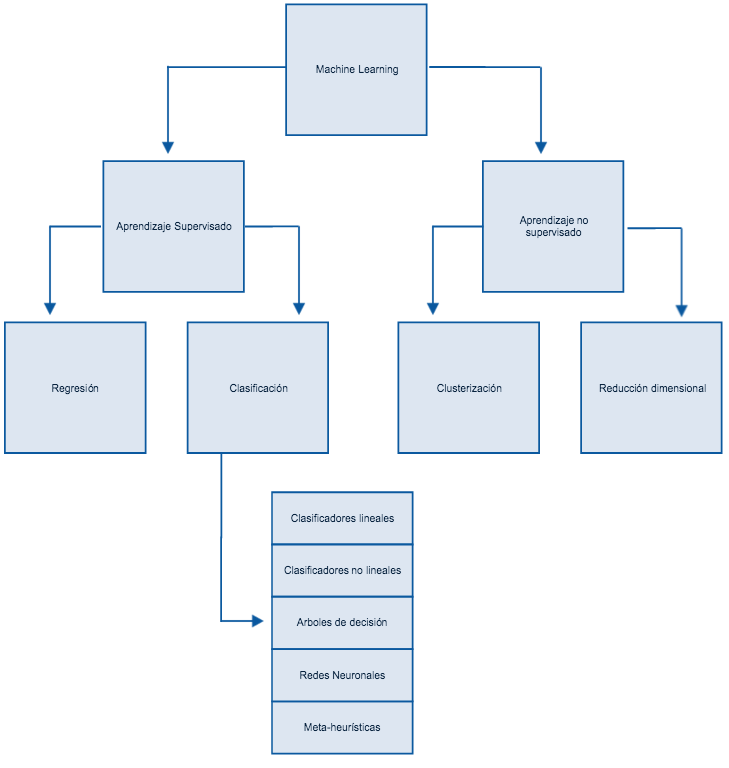
\includegraphics[width=1\textwidth]{Figures/Chapter1_Clasificacion}	
  \caption[Types of learning and the most common methods]
  {Distinct methods to solve problems in Machine Learning}
\end{figure}

\subsection{Fase de inferencia y fase de decisión}

Como primer paso, una vez elegido el método, se selecciona el criterio de penalización de los errores. Este debe ser elegido de manera acorde al problema planteado; por ejemplo, en el caso de una regresión lineal se desea que la penalización sea mayor en los datos que queden muy lejos del ajuste lineal, por lo que se escoge la norma euclidiana \footnote{Además de que las estimaciones hechas a través de mínimos cuadrados bajo ciertos supuestos tienen propiedades deseables de los estimadores: Que sean insesgados y de varianza mínima} $||x||_2 = \sqrt[]{x_{1}^{2}+x_{2}^{2}+ ... + x_{n}^{2}}$. En cambio, en un problema de clasificación se escoge una matriz de penalización o matriz de pérdida, en la que se establece el costo por cada tipo de error de clasificación.

Como segundo paso, se procede con la fase de inferencia, en la que se ajustan los estimadores de los parámetros del modelo elegido de acuerdo a los datos que se tienen, esto con el fin de hacer la inferencia de las distribuciones poblacionales. Como tercer y último paso, se procede a la fase de decisión, en la que se busca encontrar un criterio de decisión que minimice la pérdida esperada \cite{bishop2006pattern}. Por ejemplo, para los problemas de clasificación es muy claro determinar estas dos fases: la primera, se lleva a cabo al determinar la distribución conjunta de clases de pertenencia e individuos; mientras que la segunda, se realiza al determinar las fronteras de decisión basadas en estas probabilidades. Por otra parte, para los problemas de regresión tradicional, ambas fases se realizan al mismo tiempo, ya que al calcular los estimadores de los parámetros se utiliza el método de mínimos cuadrados que minimiza la penalización cuadrática.


\section{Clasificación con modelos lineales}


Se comenzará definiendo la nomenclatura utilizada en esta tesis. Las clases se denotan con la variable aleatoria $k \in C$, con $C  = \{ k = k_j: j = 1, \vdots, K\}$ el conjunto de posibles clases a clasificar y $n(C) = K$ la cardinalidad del conjunto. Para los individuos se define la variable aleatoria $x \in {\rm I\!R}^{m}$. De esta manera, sea $p(x, k)$ \footnote{Teniendo esta probabilidad se pueden calcular fácilmente las probabilidades condicionales $p(k|x)$ y $p(x|k)$} la distribución conjunta de individuos $x$ con clases $k$.


Para la fase de inferencia se utilizan los datos de entrenamiento, donde se distingue a los individuos y a sus clases de pertenencia $x_i \in  {\rm I\!R}^{m}$ y $y_i \in {\rm I\!R}$ respectivamente, con $i = 1, ... , N$. Agrupándolos en matrices, sea $X \in {\rm I\!R}^{N \times m}$ la matriz de individuos y $Y \in {\rm I\!R}^{N \times 1}$ el vector de clases de pertenencia asociada a cada individuo. Una vez hecha la inferencia, se pueden encontrar clases predichas para los individuos $x_i$, se denotará como $\widehat{y_i}$ y $\widehat{Y}$ a la respectiva matriz.


\begin{table}
\caption{Nomenclatura usada en el texto}
\begin{center}
    \begin{tabular}{ | l | c | c | p{4.5cm} |}
    \hline
    Tipo & Definición & Valores & Descripción  \\ \hline
    Entero & $K$ & $K \in \mathbb{N}$ & Número de posibles clases. \\ \hline
    Entero & $N$ & $N \in \mathbb{N}$ & Número de individuos en los datos. \\ \hline
    Entero & $N_k$ & $N_k \in \mathbb{N}$ & Número de individuos en la clase $k$. \\ \hline
    Entero & $m$ & $m \in \mathbb{N}$ & Dimensión de los individuos. \\ \hline
    v.a. & $k$ & $k \in C$ & Variable aleatoria de las clases. \\ \hline
	v.a. & $x$ & $K \in {\rm I\!R}^{m}$ & Variable aleatoria de los individuos. \\ \hline
    Conjunto & $C$ & $k_j: j = 1 ... K$ & Conjunto de posibles clases. \\ \hline
    Dato & $x_i$ & $x_i: i = 1 ... N$ & Vector columna del individuo $i$. \\ \hline
    Dato & $y_i$ & $y_i: i = 1 ... N$ & Dato de clase real del individuo $i$. \\ \hline
    Dato & $\widehat{y_i}$ & $\widehat{y_i}: i = 1 ... N$ & Dato de clase predicha del individuo $i$. \\ \hline
    Dato & $X$ & $X^T = [x_1 |...| x_N]$ & Matriz de individuos. \\ \hline
    Dato & $Y$ & $Y^T = [y_1 | ... | y_n]$ & Vector de clases reales de infividuos. \\ \hline
    Datos & $\widehat{Y}$ & $\widehat{Y}^T = [\widehat{y_1} | ... | \widehat{y_n}]$ & Vector de clases predichas de infividuos. \\ \hline
    Distribución & $p(x,k) $ &  & Distribución conjunta de individuos y clases \\ \hline
    \end{tabular}
\end{center}
\end{table}


\subsection{Fase de inferencia}
Como se mencionaba antes, en fase de inferencia se busca encontrar la distribución conjunta de la muestra con cada una de las clases, es decir $p(x,k)$. La dificultad en estimar esta distribución aumenta conforme la dimensionalidad de $x$ crece y conforme el número de clases aumenta \footnote{Para poder estimar la distribución conjunta, el número de clases debe ser menor que el conjunto de individuos}. Esto es debido a que se comienza a requerir un conjunto de datos mayor para poder estimar cada punto de $p(x,k)$. Por esta razón, muchas veces es suficiente encontrar directamente $p(k|x)$; es decir, dadas las características del individuo, encontrar que tan probable es que pertenezca a cada clase. Por otro lado, en la fase de decisión se encuentra la asignación óptima dependiendo de la matriz de pérdida que se seleccionó y de las probabilidades calculadas (ya sea la distribución conjunta o las condicionales). 

Los modelos propuestos para resolver la fase de inferencia se pueden agrupar de la siguiente manera \cite{bishop2006pattern}: 

\begin{enumerate}
	\item  \textbf{Modelos Probabilísticos Generativos.}
    Plantean resolver el problema de inferencia con el objetivo de determinar $p(x,k)$; es decir, la distribución conjunta de individuos y clases. Una vez obtenida la distribución, se puede usar para calcular $p(x|k)$, $p(k|x)$, $p(x)$ o $p(k)$. Para este enfoque se tienen que hacer supuestos acerca de la distribución de $x$ o $x|k$, o bien, tener un conjunto de entrenamiento muy grande que permita inferir acertadamente $p(x,k)$.

    Tomando propiedades básicas de probabilidad, se pueden calcular las distribuciones necesarias:
  
    \begin{equation} \label{eq:1}
     p(x, k) = p(x|k) p(k)
    \end{equation}

    \begin{equation} \label{eq:2}
     p(x, k) = p(k|x) p(x) 
    \end{equation}
    
    \begin{equation} \label{eq:3}
     p(k|x)  = \frac{p(x|k)p(k)}{p(x)}
    \end{equation}

	\begin{equation} \label{eq:4}
	 p(x) = \sum_{k} p(x|k)p(k) 
	\end{equation}
	
	\begin{equation} \label{eq:5}
	 p(k) = \sum_{x} p(k|x)p(x) 
	\end{equation}
	
	En caso de no tener suficientes datos para inferir directamente esta distribución; o bien, de no tener conocimiento de la estructura de la distribución de $x$, se dan preferencia a los modelos discriminativos o modelos de funciones discriminantes.

\textit{Ventajas\cite{bishop2006pattern}:}
\begin{itemize}
\item Puede ser útil para detectar datos atípicos, ya que al supone una distribución de $x$, se puede determinar qué puntos son poco probables de suceder. De esta manera, se puede encontrar qué predicciones podrían fallar. 
\end{itemize}

\textit{Desventajas\cite{bishop2006pattern}:}
\begin{itemize}
\item Se debe tener información acerca de la distribución de $x$.

\item Inferir directamente de los datos la distribución $p(x,k)$ puede ser muy demandante cuando la dimensionalidad de $x$ es alta. 

\item Si solo se requiere hacer clasificación, puede ser ineficiente encontrar toda la distribución conjunta.
\end{itemize}


\item \textbf{Modelos Probabilísticos Discriminativos.}
Primero, se resuelve el problema de inferencia para determinar $p(k|x)$ con los datos, y después se procede a la fase de decisión para asignar la clase de pertenencia.

\textit{Ventajas:\cite{bishop2006pattern}}
\begin{itemize}
\item Solo se necesita estimar $p(k|x)$ y no toda la distribución conjunta.
\end{itemize}

\textit{Desventajas:\cite{bishop2006pattern}}
\begin{itemize}
\item No se tiene la detección de atípicos presentados por el primer enfoque.
\end{itemize}


\item \textbf{Función Discriminante}
Plantea encontrar una función $\widehat{f}:{\rm I\!R}^m \rightarrow {\rm I\!R}$, tal que clasifique directamente a cada individuo en una clase $k$, de esta manera se define $\widehat{Y}=\widehat{f}(x)$. 

\textit{Ventajas:\cite{bishop2006pattern}}
\begin{itemize}
\item Se combina la fase de inferencia y la fase de decisión en una sola función $\widehat{Y}=\widehat{f}(x)$. 
\end{itemize}

\textit{Desventajas:\cite{bishop2006pattern}}
\begin{itemize}
\item Ya no se cuenta con las probabilidades posteriores $p(k|x)$, por lo que ya no se puede analizar una a una la probabilidad de pertenencia del individuo $x$ a cada una de las clases.
\end{itemize}

\end{enumerate}


\subsection{Fase de decisión}
Para la fase de decisión es conveniente analizar tres definiciones: ``Regiones de decisión'',  ``Fronteras de decisión'' y  ``Funciones discriminantes''. Las primeras dos reciben este nombre porque buscan dividir el espacio al que pertenecen los datos en regiones distintas y excluyentes. Cada una de estas regiones $R_{k}$ clasifica al individuo $x$ en una única clase $k$. En cambio, las fronteras de decisión son las zonas que delimitan una región de las demás; es decir, en ellas (o en sus cercanías) es indiferente qué clase elegir. Por esta razón, es conveniente analizar los datos que quedan cercanos para poder hacer una elección, tomando en cuenta la naturaleza del problema. Por último, las Funciones Discriminantes, nos permiten comparar directamente qué tan verosímil es que un individuo pertenezca a una clase u a otra.

Debido a la finalidad del texto se proponen fronteras lineales \footnote{Las fronteras de decisión pueden tomar formas irregulares, pero en general su forma depende del método de clasificación elegido}, ya que al igual que una regresión lineal, es la base que ejemplifica modelos más complejos. Por este motivo, se mostrarán distintas opciones para construir las regiones y fronteras que se adecuan a los tres enfoques distintos: modelos probabilísticos generativos, modelos probabilísticos discriminativos y funciones discriminantes. 

Para asegurar la linealidad en las fronteras, se debe hacer un análisis que garantice esta propiedad. Se ejemplificará con un caso de dos clases: $k_i$ y $k_j$ con $\left( \begin{array}{ccc}
0 & c_{ij} \\
c_{ji} & 0 \\
 \end{array} \right)$, la matriz de costos con $c_{ij}$ el costo de elegir $i$ cuando la verdadera clase es $j$. Se supone que $c_{ij}, c_{ji}$ mayores que 0. De esta manera la frontera de decisión está dada por:

\begin{equation} \label{eq:6}
c_{ij} p( k = k_i | x \in k_j) - c_{ji} p(k = k_j| x \in k_i) = 0
\end{equation}

De otra manera, si $c_{ij} p( k = k_i | x \in k_j) < c_{ji} p( k = k_j| x \in k_i) $ o viceversa, entonces se clasificará hacia $k_i$ y $k_j$, respectivamente. Para los fines de esta tesis, se tomarán los costos de $c_{ij} = c_{ji} = 1$ ya que esto solo juega en la ordenada al origen de la ecuación de la frontera lineal. Tomando un resultado presentado por T. Mitchell \cite{mitchell2006discipline}, si se aplica una función monótona de $p(k, x)$, la linealidad de las fronteras de decisión se mantiene. En este caso, se toma la función de logaritmo $log()$:


$$ log(p(k = k_j | x)) = log( p(k = k_i | x)) $$	

\begin{equation} \label{eq:7}
 log \frac{p( k = k_j | x )}{ p(k =  k_i |  x)} = 0 	
\end{equation}

El lado izquierdo de esta última ecuación es conocido como razón de momios (log odd). Cuando es una función lineal con respecto a $x$, mantiene la linealidad de la frontera:

\begin{equation} \label{eq:8}
 log \frac{p(k = k_j | x )}{p(k = k_i |  x)} = \beta_0 + x^T \beta_1 
\end{equation}


\section{Métodos de clasificación lineales}

En la fase de inferencia se busca construir la distribución $p(x,k)$, la cual será usada en la fase de decisión para tomar un criterio óptimo de clasificación. En la sección 2.2 se mostraron los distintos enfoques que se toman para hacer esta inferencia. Recapitulando, para modelos generativos se escoge $\widehat{Y}(x) = \widehat{f}(p(x,k))$; para modelos discriminativos $\widehat{Y}(x) = \widehat{f}(p(k|x))$ y para funciones discriminantes se escoge $\widehat{Y}(x)$ = $\widehat{f}(x)$. En los dos primeros casos se ve que la función $f$ toma como entrada distribuciones concernientes a $x$ y $k$, pero en el tercer caso, solamente toma como entrada a $x$. En esta sección se ejemplificarán los 3 métodos con técnicas sencillas. Para el enfoque Probabilístico Generativo se empleará el Análisis Discriminante Lineal, para el Probabilístico Discriminativo la Regresión Logística y para la función discriminante, el Discriminante Lineal de Fisher.

En los siguientes tres ejemplos se explica cómo se realiza la inferencia de las distribuciones, para después demostrar la linealidad en las fronteras. Como se explica en la sección 2.2.2, si se asegura que (\ref{eq:8}) es lineal con respecto a $x$, entonces se garantiza la linealidad de estas. En la Regresión Logística se ejemplificará el procedimiento para $n$ clases. Para los demás se supondrá el caso de la frontera entre dos clases.


\subsection{Modelos discriminativos: Regresión Logística}


\textit{Inferencia de la distribución $p(k | x)$} \\
Para la fase de inferencia, se calculan las probabilidades posteriores de pertenecer a cada grupo $j$, de manera que: 
\begin{equation} \label{eq:15}
	\sum\limits_{j = 1}^{K} p(k = k_j | x) = 1
\end{equation}


\textit{Linealidad de la frontera}\\
Para obtener la estimación de las $K$ distribuciones de probabilidad $p(k = k_j | x)$, se parte de la ecuación (\ref{eq:8}) y se supone que todas las fronteras son lineales.

$$ \log \frac{p(k = k_1 | x)}{p(k = k_K | x)} = \beta_{1.0} + \beta_1^T x$$

$$ \log \frac{p(k = k_2 | x)}{p(k = k_K | x)} = \beta_{2.0} + \beta_2^T x$$

$$\vdots$$

$$ \log \frac{p(k = K-1 | x)}{p(k = k_K | x)} = \beta_{(K-1).0} + \beta_{(K-1)}^T x$$

Con estas ecuaciones se crea un sistema que cuenta con $K$ variables $p(k = k_j| x)$ y $K-1$ ecuaciones, lo cual, añadiendo la restricción (\ref{eq:15}) se puede despejar cada probabilidad: 

$$ p(k = k_1 | X = x) = \frac{\exp(\beta_{1.0} + \beta_1^T x)}{1+\sum\limits_{i=1}^{K-1} {\exp(\beta_{l.0} + \beta_l^T x)}} $$

$$ p(k = k_2 | X = x) = \frac{\exp(\beta_{2.0} + \beta_2^T x)}{1+\sum\limits_{i=1}^{K-1} {\exp(\beta_{l.0} + \beta_l^T x)}} $$

$$ \vdots $$

$$ p(k = k_{K-1} | X = x) = \frac{\exp(\beta_{(K-1).0} + \beta_{(K-1)}^T x)}{1+\sum\limits_{i=1}^{K-1} {\exp(\beta_{l.0} + \beta_l^T x)}} $$

Para la clase de referencia: 

$$ p(Y = k_K | X = x) = \frac{1}{1+\sum\limits_{i=1}^{K-1} {\exp(\beta_{l.0} + \beta_l^T x)}} $$

Para tener la formulación completa, falta estimar las $\beta$ de cada probabilidad. Esto, comúnmente, se realiza con máxima verosimilitud (a través de métodos iterativos como Newton) \cite{hastie2009elements}


\textit{Funciones $logit$ y $logit^{-1}$} \\
Para este modelo es conveniente analizar la función logit y su inversa:
 
 \begin{equation} \label{eq:16}
 logit = \log (\frac{p}{1-p}) 
 \end{equation}

\begin{equation} \label{eq:17}
 logit^{-1}  = \frac{\exp(x)}{1+\exp(x)}
 \end{equation}


Al graficar la función $logit$ y la $logit^{-1}$ sobre un plano (Figura 1.1) se observan algunas de sus propiedades. En la gráfica de la izquierda, se realiza un mapeo de valores del rango (0,1) al rango (-$\inf$,$\inf$), mientras que a la derecha se transforman valores continuos de (-$\inf$, $\inf$) al $(0,1)$. La transformación realizada por $logit^{-1}$ es de mayor interés ya que su rango es semejante al que toman las probabilidades. Este enfoque nos da una amplia gama de elección para la fase de decisión, ya que deja elegir los puntos de corte para cada clase, dependiendo la penalización que se quiera dar a cada tipo de error \cite{hastie2009elements}:

\begin{figure}[!ht]
  \centering
	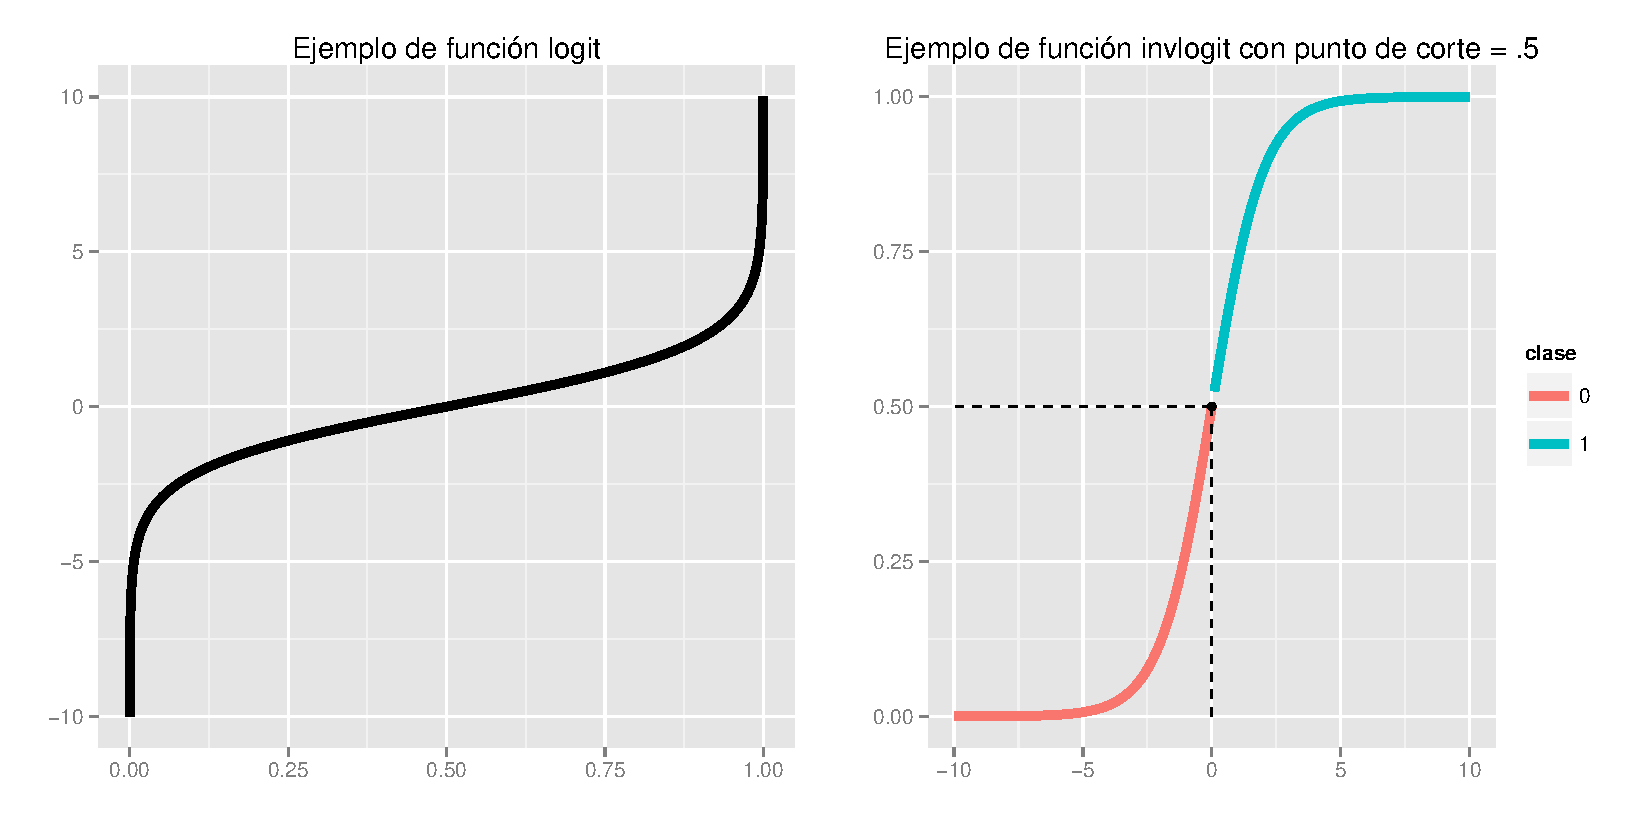
\includegraphics[width=1\textwidth]{Figures/Chapter1_logit}	
  \caption[Función logit y $logit^{-1}$]
  {En la izquierda se muestra la función logit y en la derecha la función $logit^{-1}$ con punto de corte p = .5; es decir, se escoge la clase 1 en la zona azul y la clase 0 en la zona roja.}
\end{figure}

\pagebreak
\subsection{Modelos generativos: Análisis Discriminante Lineal}


\textit{Inferencia de la distribución $p(x,k)$}\\
Para el caso del Análisis Discriminante Lineal se sigue un enfoque generativo, en el que se realiza inferencia de $p(x,k)$. Primero, se supondrá que $p(x|k)$ sigue una distribución Gaussiana con varianza $\Sigma_{k}$ constante para todas las clases y $\mu_{k}$ la media de los individuos pertenecientes a la clase $k$ (ecuación (\ref{eq:9})). Por otra parte, se estima la distribución $p(k)$ como la proporción de casos que cada clase aparece en los datos (ecuación (\ref{eq:10})). Usando la ecuación (\ref{eq:1}) se deduce $p(x,k)$:


\begin{equation} \label{eq:9}
 p(x|k) = \frac{1}{(2\pi) |\Sigma|^{1/2}} e^{-\frac{1}{2}(x-\mu_{k})^{T}\Sigma^{-1}(x-\mu_{k})}
\end{equation}

\begin{equation} \label{eq:10}
 p(k) = \frac{N_k}{N}	
\end{equation}

Por otro lado, al utilizar el Teorema de Bayes (\ref{eq:3}) y la ecuación (\ref{eq:4}), se puede calcular $p(k|x)$ directamente. 



\textit{Linealidad de la frontera}\\
Al hablar de la linealidad de la frontera, se tiene que cumplir la ecuación (\ref{eq:8}), enunciada en la sección 2.2.2:

$$\log \frac{p(k = k_j | x )}{p(k = k_i |  x)} = \beta_0 +  x^T \beta_1$$

$$\log \frac{p(x | k = k_j)p(k = k_j)}{p( x | k = k_i)p(k = k_i)} = \beta_0 +  x^T \beta_1$$

\begin{equation} \label{eq:11}
 	\log\frac{p(x | k = k_j)}{p(x | k = k_i)} + \log\frac{p(k = k_j)}{p(k = k_i)} = \beta_0 +  x^T \beta_1
\end{equation} 

La ecuación (\ref{eq:11}) consta de dos sumandos. Al desarrollar el primero:

$$ \log\frac{p(x | k = k_j)}{p(x | k = k_i)} = -\frac{1}{2}[(x - \mu_j)^T \Sigma^{-1}(x - \mu_j) - (x - \mu_i)^T \Sigma^{-1}(x - \mu_i)] $$ 


\begin{equation}
\begin{aligned}
 \log\frac{p(x | k = k_j)}{p(x | k = k_i)} =& -\frac{1}{2}[{\mu_j}^T \Sigma^{-1} {\mu_j}  -  {\mu_i}^T \Sigma^{-1} {\mu_i}]  + \\
 &\frac{1}{2}[{x}^T \Sigma^{-1}(\mu_j-\mu_i) - {(\mu_j-\mu_i)}^T \Sigma^{-1}(x)
\end{aligned}
\end{equation}

 

 \begin{equation} \label{eq:12}
 	\log\frac{p(x| k = k_j)}{p(x | k = k_i)} = -\frac{1}{2}[{(\mu_j - \mu_i)}^T \Sigma^{-1} {(\mu_j + \mu_i)}] + [{x}^T \Sigma^{-1}(\mu_j-\mu_i)]
 \end{equation}

Sustituyendo \ref{eq:12} en \ref{eq:11} se tiene como resultado:

$$ \log \frac{p(k = k_j)}{p(k = k_i)} - \frac{1}{2}[(\mu_j - \mu_i)^T \Sigma^{-1} (\mu_j + \mu_i)] + {x}^T \Sigma^{-1} (\mu_j - \mu_i) = \beta_0 +  x^T \beta_1$$

Del cual se nota que $\beta_0$ y $\beta_1$ son equivalentes a:

\begin{equation} \label{eq:13}
\beta_0 = \log \frac{p(k = k_j)}{p(k = k_i)} - \frac{1}{2}[(\mu_j - \mu_i)^T \Sigma^{-1} (\mu_j +\mu_i)] 	
\end{equation}

\begin{equation} \label{eq:14}
 \beta_1 = \Sigma^{-1} (\mu_j -\mu_i)
\end{equation}


\textit{Funciones Discriminantes} \\
Ahora, solo falta enunciar las funciones discriminantes de la clase $i$ y $j$; es decir, $log p(k = k_i | x)$ y  $log p(k = k_j | x)$, respectivamente:
$$ \delta_j (x) = \log {p(k = k_j)} - \frac{1}{2}\mu_j^T \Sigma \mu_j + x^T \Sigma^{-1} \mu_j$$
$$ \delta_i (x) = \log {p(k= k_i)} - \frac{1}{2}\mu_i^T \Sigma \mu_i + x^T \Sigma^{-1} \mu_i$$


\subsection{Funciones Discriminantes: Discriminante Lineal de Fisher}

El Discriminante Lineal de Fisher es similar al Análisis Discriminante Lineal. El primero permite ver una proyección informativa en un espacio de dimensión menor \cite{hastie2009elements}. Este planteamiento fue propuesto por Fisher \cite{fisher1936use}, y hace referencia a un discriminante lineal con menos supuestos \footnote{No toma en cuenta la distribución de los datos, ni la igualdad de varianzas entre las clases.}. Propone los supuestos de definir una varianza entre clases que es la varianza de las medias de las clases, y una varianza intra-clase, que mide la varianza dentro de las clases con respecto a la media de cada clase. Después, se busca una matriz de proyección $V$ que maximice la dispersión entre-clase al mismo tiempo que minimiza la dispersión intra-clase \cite{ngo2012trace}.

Se comenzará definiendo la nomenclatura necesaria para la sección. Sea $N_{k}$ el número de personas en la clase $k$, $N$ el número total de personas y $w_i = V^T x_i$; es decir, los datos proyectados con la matriz $V$. Entonces, se definen las medias de grupo $k$ como $\mu_k$ y la media de todos los datos $x_i$ como $\mu$:

\begin{equation} \label{eq:18}
 	\mu_k = \frac{1}{N_{k}} 
 	\sum_{\substack{i = 1\\
                  	y_i = k}}^{N}
                  x_i
\end{equation} 


\begin{equation} \label{eq:19}
 \mu = \frac{1}{N} \sum_{i = 1}^{N} x_i
\end{equation}

Por otro lado, se definen las medias correspondientes a los datos proyectados $w_i$:
\begin{equation} \label{eq:20}
 	\widetilde{\mu_k} = \frac{1}{N_{k}} 
 	\sum_{\substack{i = 1\\
                  	y_i = k}}^{N}
                  w_i
\end{equation} 


\begin{equation} \label{eq:21}
 \widetilde{\mu} = \frac{1}{N} \sum_{i = 1}^{N} w_i
\end{equation}


La matriz de dispersión intra-clase de los datos proyectados:


$$\Phi_{I} = \sum_{k=1}^{K} 
				\sum_{\substack{i = 1\\
                  			   	y_i = k}}
                    ^{N}
           ||w_i-\widetilde{\mu}_{k}||^{2}_{2}$$


$$ \Phi_{I} =  \sum_{k=1}^{K} 
					\sum_{\substack{i = 1\\
                  			   	y_i = k}}
                    ^{N}
			Tr (V^T (x_i - \mu_k)(x_i - \mu_k)^T V ) $$

\begin{equation} \label{eq:22}
 \Phi_{I} =  Tr(V^T S_I V) 
\end{equation}



\begin{equation} \label{eq:23}
con \quad S_I = \sum_{k=1}^{K} 
					\sum_{\substack{i = 1\\
                  			   	y_i = k}}
                    ^{N}
 ({x_i-\mu_{k}})({x_i-\mu_{k}})^T 
\end{equation}



La matriz de dispersión entre-clases de los datos proyectados:

$$ \Phi_{E} = \sum_{k=1}^{K} N_{k} || \widetilde{\mu}_k - \widetilde{\mu} ||^{2}_{2} $$

$$ \Phi_{E} = \sum_{k=1}^{K} N_{k} || V^T \mu_k - V^T \mu ||^{2}_{2} $$
 
$$ \Phi_{E} =  \sum_{k=1}^{K} N_{k} V^T(\mu_k - \mu)(\mu_k - \mu)^T V $$
\begin{equation} \label{eq:24}
 \Phi_{E} =  Tr(V^T S_E V)  
\end{equation}

\begin{equation} \label{eq:25}
 con \quad S_E = \sum_{k=1}^{K} N_{k} (\mu_k - \mu)(\mu_k - \mu)^T 
\end{equation}

De este modo, se definen las dos matrices importantes del método: $S_I$ la matriz de dispersión interna y $S_E$ la matriz de dispersión entre clases. Con estas definiciones surge la idea intuitiva de maximizar $\Phi_{E}$ al mismo tiempo que se minimiza $\Phi_{I}$; es decir, encontrar un espacio de proyección en el que los grupos pertenecientes a la misma clase tengan poca varianza, al mismo tiempo que la varianza entre estas clases sea alta. Se puede plantear esta idea a través del problema de maximización:

\begin{equation}\label{eq:26}
	\max_{\substack{V \in {\rm I\!R}^{n\times p} \\ V^TV = I}} \frac{Tr(V^T S_E V)}{Tr(V^T S_I V)} 
\end{equation}

Este problema de optimización es el principal tema de la tesis, por lo que los detalles acerca de las fronteras y el proceso de maximización que derivan en encontrar la matriz óptima $V$ será analizado en los capítulos siguientes.

\section{Enfoques para la minimización del error}

La teoría de la decisión se aplica para la fase dos, en la que se busca tomar decisiones óptimas dadas las probabilidades calculadas en la fase de inferencia. La motivación de una teoría de la decisión es que las probabilidades, por sí solas, no nos indican que clase elegir, solamente nos dan información del comportamiento de la distribución. Por esta razón, es conveniente saber que decisión tomar basándonos en la penalización de los errores elegidos anteriormente. Puede verse desde dos perspectivas \footnote{En realidad el primer enfoque es un caso particular del segundo}:

\begin{itemize}
\item Minimizar el error de clasificación a lo largo de todos nuestros datos.
\item Minimizar la pérdida esperada dada una matriz de pérdida L. 
\end{itemize}


\subsection{Minimizando el error de clasificación}
Esta regla dividirá el espacio en regiones $R_j$ en las que cada individuo es asignado a una clase $k_j$ con $j = 1, ... , K$. Recordando la nomenclatura, $x_i$ es el individuo $i$ y $y_i$ es la clase a la que pertenece este sujeto; mientras que $\widehat{y}_i$ es la clase predicha del sujeto $i$. Por otro lado, $k_j$ es la clase $j$ de las $K$ existentes. Para encontrar la decisión óptima de elección se busca minimizar la probabilidad de cometer errores, que está dada por:

%$$p(error) = 1 - \sum_{i = 1}^{N} \sum_{j=1}^{K} p(y_i = k_j, \widehat{y}_i = k_j)$$


$$p(error) = 1 - \sum_{i = 1}^{N} \sum_{j=1}^{K} p(x_i \in R_{j}, y_i = k_j)$$

En la expresión anterior, cuando $x_i \in R_j$ se sabe que $\widehat{y}_i$ esta asociada a la clase $k_j$. Ocupando la igualdad $p(x \in R_{j}) = \int_{R_j} p(x) dx$ se tiene que es equivalente a maximizar la probabilidad de no cometer errores:

$$p(no error) = \sum_{i = 1}^{N} \sum_{j=1}^{K} p(x_i \in R_{j},  y_i = k_j)$$

$$p(no error) = \sum_{i = 1}^{N} \sum_{j=1}^{K} \int_{R_j} p(x_i, y_i = k_j) dx $$

Es facil deducir que $\int_{R_j} p(x_i, y_i = k_j) dx$ es equivalente a que $p(\widehat{y}_i = k_j, y_i = k_j)$ porque cuando $x_i$ está en la región $R_j$, entonces $\widehat{y}_i = k_j$. Ocupando esta igualdad se puede deducir:

\begin{equation}\label{eq:27}
p(no error) = \sum_{i = 1}^{N} \sum_{j=1}^{K} p(\widehat{y}_i = k_j, y_i = k_j) 
\end{equation}

Es decir, dado que $x_i$ pertenece a la región $R_{j}$ (y por lo tanto es clasificado en la clase $k_j$) y la clase original de $x_i$ es $y = k_j$, implica que la clasificación es correcta. La maximización de (\ref{eq:27}) sigue un argumento intuitivo. Al obtener la distribución $p(x, k)$, se selecciona aquella que tiene la probabilidad más alta de ocurrir para cada individuo; es decir, tomar como criterio de decisión la que tenga mayor $p(x_i \in R_j)$. 

En los Modelos Probabilísticos Generativos se utiliza la distribución conjunta, en cambio en los discriminativos solamente se utiliza $p(k|x)$. Para extender el resultado anterior a la distribución condicional se ocupa la ecuación $\ref{eq:2}$:

$$p(x,k)  = p(k|x)p(x)$$

Maximizar $p(x,k)$ es equivalente a maximizar el término de la derecha. Como $p(x)$ es positivo y común a todos los términos, es equivalente a seleccionar la clase con probabilidad $p(k|x)$ más grande para cada individuo. 

\subsection{Minimizando la pérdida esperada}

Tomando una matriz de pérdida se puede ver más general el error de clasificación. La motivación de este enfoque es la disparidad en los distintos costos asociados a cada tipo de error de clasificación. Por ejemplo, en un problema en el que se predice si a un paciente le dará un ataque al corazón, es peor predecir que no tendrá un ataque cuando en realidad si lo tendrá \cite{hastie2009elements}. Por esta razón, la modelación del error a través de una matriz de pérdida tiene sentido. Sea $L$ la matriz que tiene como característica el tener ceros en la diagonal y pesos no negativos en cualquier otro lado y $L(X,Y)$ el costo asociado a elegir Y cuando la clase verdadera es X. \footnote{Es fácil notar que la matriz $L_{0-1}$; es decir, 0 sobre la diagonal (Clasificación correcta) y 1 (Clasificación incorrecta) en cualquier otro lugar, es equivalente al enfoque que minimiza el error de clasificación}

Tomando el error esperado de predicción de los vectores $Y$ y $\widehat{Y}$ bajo la matriz $L$:

$$ EEP = E[L(Y, \widehat{Y})] $$

En la que $Y$ es el vector de clases de pertenencia verdaderas y $\widehat{Y}$ es el vector de clases de pertenencias predichas. Ambos vectores son de variables categóricas que pueden tomar valores $k_j \in C$ con $j = 1 ... K$. 

Al desarrollar el error esperado de predicción como una sumatoria sobre los $N$ individuos y las $K$ clases, es equivalente a:

$$EEP = \sum_{i = 1}^{N} \sum_{j=1}^{K} L[y_i = k_j, \widehat{y}_i = k_j] p(x = x_i, k = k_j)$$

Sustituyendo $p(k, x) = p(k | x)p(x)$, se puede calcular la esperanza sobre los individuos $x$. Lo que se deduce la expresión:

$$EEP = E_{x} \sum_{j=1}^{K} L[y = k_j, \widehat{y} = k_j] p(k_j | x)$$

Como se busca minimizar el error esperado de predicción con respecto a $\widehat{y}$, se obtiene el siguiente problema de minimización:

$$\widehat{y}^{*} = \argmin_{\widehat{y}} E_{x} \sum_{j=1}^{K} L[y = k_j, \widehat{y} = k_j] p(k_j | x)$$

Este problema de minimización es equivalente a minimizar el error esperado de predicción para cada individuo $x$:

$$\widehat{y}^{*} = \argmin_{\widehat{y}} \sum_{j=1}^K L[y = k_j, \widehat{y} = k_j]p(k_j|x)$$

Al escoger la función de pérdida $0-1$, cuando $\widehat{y}^{*} = y$, entonces la pérdida es igual a 0, por lo que la fórmula se simplifica a:

$$\widehat{y}^{*} = \argmin_{\widehat{y}}
\sum_{\substack{j = 1 \\
			   y \neq \widehat{y}}} ^ K 
			   L[y = k_j, \widehat{y} = k_j] p(k_j | x)$$

Por otro lado, cuando $\widehat{y}^{*} \neq y$ entonces la pérdida es igual a 1:

$$\widehat{y}^{*} = \argmin_{\widehat{y}}
\sum_{\substack{j=1 \\
      y \neq \widehat{y}}}^K
p(k_j | x)$$

$$\widehat{y}^{*} = \argmin_{\widehat{y}} 
[1 - \sum_{\substack{j=1 \\
      y = \widehat{y}}}^K
p(k_j|x)]$$

Esta expresión es equivalente a maximizar:

$$\widehat{y}^{*} = \argmax_{\widehat{y}} p(k|x)$$

De esta manera, se escoge $\widehat{y}^{*}$ como la probabilidad posterior más grande de pertenencia a la clase $k$ dado $x$. Esta solución es conocida como ``Clasificador de Bayes'' y nos dice que hay que clasificar a las clases más probables usando la distribución condicional $p(k|x)$. La tasa de error de este clasificador se le conoce como ``Tasa de Bayes''\cite{hastie2009elements}.



 
	%  \chapter{Discriminante Lineal de Fisher}
\label{ch:chapter2}

En este capítulo se hablará del Análisis Discriminante Lineal de Fisher (ADLF), el cual busca optimizar un cociente de la forma $Tr(V^T A V) / Tr(V^T B V)$ sobre el conjunto de matrices ortogonales $V$ con $A, B$ matrices positivas definidas. Para resolver el ADLF, se han presentado en libros de aprendizaje estadístico y clasificación de patrones formulaciones alternas al problema original, ya que este era considerado computacionalmente muy costoso \cite{wang2007trace}\cite{ngo2012trace}. Planteamientos como: maximizar la traza de la matriz de dispersión entre clases sujeto a una restricción sobre la matriz de dispersión interna, maximizar la traza del cociente de matrices; o bien, maximizar el cociente de determinantes, han sido formulaciones presentadas en distintos textos \cite{duda2012pattern} \cite{hastie2009elements} \cite{mitchell2006discipline} \cite{fukunaga2013introduction}. Al final, todas estas propuestas resultan ser versiones simplificadas del problema.

En este capítulo se resolverá el problema original del ADLF a través del método de Newton-Lanczos, el cual resulta ser computacionalmente eficiente. En la primer sección del capítulo se contextualizará al problema dentro del área de Aprendizaje de Máquina. En la segunda parte, se proporcionará la teoría correspondiente para seguir con facilidad el texto. Por último, en la tercera parte, se plantea la solución al problema de ADLF para una dimensión, se generaliza a $p$ dimensiones y se proporcionan las condiciones para la existencia de la solución.


\section{Aprendizaje de máquina}
El Aprendizaje de Máquina toma como base dos áreas de investigación: la Ciencia de la Computación y la Estadística. De la primera, retoma las preguntas: ¿Cómo se pueden construir máquinas que resuelvan problemas? Y ¿Qué problemas son tratables o intratables? De la segunda, toma las preguntas: ¿Qué puede ser inferido de los datos? ¿Bajo que supuestos del modelo? Y ¿Con qué confiabilidad? \cite{mitchell2006discipline}. El esfuerzo por resolver estas preguntas da como resultado una disciplina enfocada a construir teorías estadístico-computacional de los procesos de aprendizaje.

\subsection{Procesos de aprendizaje}

Se dice que una máquina ``aprende" dada una tarea (T), una medición del rendimiento (R) y un tipo de experiencia (E) si el sistema mejora confiablemente su rendimiento (R) en la tarea (T) dada la experiencia (E) \cite{mitchell2006discipline}. Es decir, se modela una estructura con los datos proporcionados de manera que el rendimiento en la tarea mejora conforme más información recibe. La diversidad de las tareas, así como el campo de aplicaciones es muy diverso, por ejemplo:

\begin{itemize} 

\item \textit{Clasificación de spam/no-spam}, en el que (E) son los correos, (T) el clasificar correctamente el \textit{spam} y (R) el porcentaje de correos correctamente clasificados.

\item \textit{Reconocimiento/Clasificación facial}, en el que (E) son los rostros de distintas personas, (T) el reconocimiento o clasificación de los rostros y (R) el porcentaje de rostros correctamente reconocidos o clasificados.
\end{itemize} 

Los procesos de aprendizaje tienen diversas aplicaciones y distintos supuestos, por lo que han surgido clasificaciones para analizarlos en conjunto. La utilizada en este texto es la propuesta por T. Hastie \cite{hastie2009elements}, la cual divide a los métodos en dos grupos: aprendizaje supervisado y aprendizaje no supervisado. El primero, supone la presencia de una variable de salida que actúa como guía en la construcción de la estructura. Ejemplos de éste es la regresión lineal, los árboles de decisión y las máquinas de soporte vectorial. 
Por otra parte, el aprendizaje no supervisado solo cuenta con la información de las variables independientes; por ejemplo, análisis de conglomerados, reglas de asociación y reducción dimensional. 

Después de esta primer clasificación, se subclasifica a los métodos de aprendizaje supervisado de acuerdo al tipo de variable de salida (Figura 1.1). \footnote{A lo largo del texto se usará indiferentemente variable de entrada como ``input'' o variable independiente y variable de salida como ``output'' o variable dependiente} Cuando se trata de una variable cuantitativa recibe el nombre de regresión, mientras que en el caso de cualitativas se le llama clasificación. Por otra parte, el aprendizaje no supervisado tiene dos ramas en las que el texto hace énfasis \cite{hastie2009elements}: Segmentación en el caso que se desee asignar un grupo a cada individuo, de manera que los grupos sean homogéneos entre sí; o bien, reducción dimensional cuando solamente se desea proyectar a los individuos en un espacio de menor dimensión, de manera que se cumplan características especiales en dicho subespacio. 

El problema de ADLF pertenece a la rama de aprendizaje supervisado, en particular a los métodos clasificación. Alternativas para esta finalidad, y que sigan asumiento linealidad en la frontera, son la Regresión Logística, el Análisis Discriminante Lineal y las Máquinas de Soporte Vectorial. 

\begin{figure}[!ht]
  \centering
  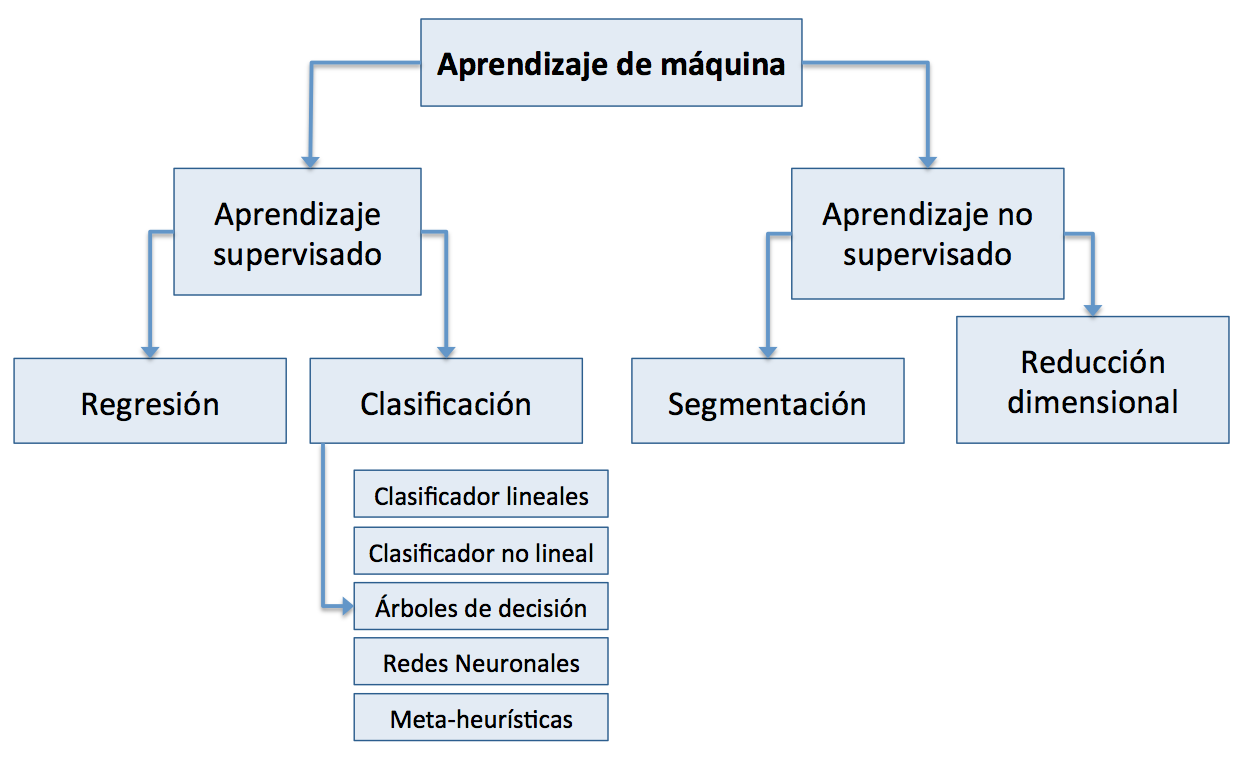
\includegraphics[width=1\textwidth]{Figures/Chapter1_Clasificacion1.png} 
  \caption[Enfoques para resolver problemas de clasificación.]
  {Distintos enfoques para resolver problemas de clasificación en el área de Aprendizaje de Máquina.}
\end{figure}

\section{Matrices de dispersión}
Se comenzará definiendo la nomenclatura necesaria para la sección. Sea $x_i$ el individuo $i$ que pertenece a la clase $y_i$, $N_{k}$ el número de personas en la clase $k$, $N$ el número total de personas y $w_i = V^T x_i$; es decir, los datos proyectados con la matriz $V$. Entonces, se definen las medias de grupo $k$ como $\mu_k$ y la media de todos los datos $x_i$ como $\mu$:

\begin{equation} \label{eq:18}
  \mu_k = \frac{1}{N_{k}} 
  \sum_{\substack{i = 1\\
                    y_i = k}}^{N}
                  x_i
\end{equation} 

\begin{equation} \label{eq:19}
 \mu = \frac{1}{N} \sum_{i = 1}^{N} x_i
\end{equation}

Por otro lado, se definen las medias correspondientes a los datos proyectados $w_i$:
\begin{equation} \label{eq:20}
  \widetilde{\mu_k} = \frac{1}{N_{k}} 
  \sum_{\substack{i = 1\\
                    y_i = k}}^{N}
                  w_i
\end{equation} 

\begin{equation} \label{eq:21}
 \widetilde{\mu} = \frac{1}{N} \sum_{i = 1}^{N} w_i
\end{equation}

El ADLF hace amplio uso de las matrices de dispersión, en específico de la matriz de covarianza, la matriz de dispersión de todos los individuos, la matriz de dispersión interna y la matriz de dispersión entre clases. Es importante analizar a profundidad la terminología y las fórmulas que se usarán a lo largo de la tesis para entender la lógica detrás de la formulación.

Sea $\Sigma$ la matriz de covarianza (\textit{Covariance Matrix)} de todos los individuos. Se define como $\widehat{\Sigma}$ al estimador insesgado de $\Sigma$ el cual está escalada entre $N-1$:

\begin{equation} \label{eq:2.1}
\widehat{\Sigma} = \frac{1}{N-1} \sum_{i=1}^{N}(x_i - \mu)(x_i - \mu)^T	
\end{equation}

Si esta matriz no está escalada por $N-1$ entonces se le conoce como matriz de dispersión (\textit{Scatter Matrix}), en esta tesis se representará como $S_T$, con el subíndice $T$ que significa que está tomando en cuenta a todos los individuos:

\begin{equation} \label{eq:2.2}
S_T = \sum_{i=1}^{N}(x_i - \mu)(x_i - \mu)^T	
\end{equation}

Cuando solo se toman a los individuos de una clase particular $k$, se puede encontrar su correspondiente matriz de dispersión, representada como $S_k$, con el subíndice $k$ simbolizando que está tomando en cuenta solo a los individuos de la clase $k$:

\begin{equation*}
S_k = \sum_{\substack{i=1 \\ y_i = k}}^{N} (x_k - \mu)(x_k - \mu)^T	
\end{equation*}

De esta manera se define la matriz de dispersión interna (\textit{Within-class scatter matrix}) como la suma sobre $k$ de todas las matrices de dispersión de cada clase:

\begin{equation}\label{eq:2.3}
S_I = \sum_{k=1}^{K} 
					\sum_{\substack{i = 1\\
                  			   	y_i = k}}
                    ^{N}
 ({x_i-\mu_{k}})({x_i-\mu_{k}})^T 	
\end{equation}

Ahora solo falta definir la matriz de dispersión entre clases (\textit{Between-class scatter matrix}) como la suma de diferencias al cuadrado de las medias de clase contra la media de todos los datos multiplicada por el número de individuos en cada clase $N_k$:

\begin{equation} \label{eq:2.4}
S_E = \sum_{k = 1}^K N_k (\mu_k - \mu)(\mu_k - \mu)^T	
\end{equation}

\begin{figure}[!ht] \label{Fig1.1}
  \centering
	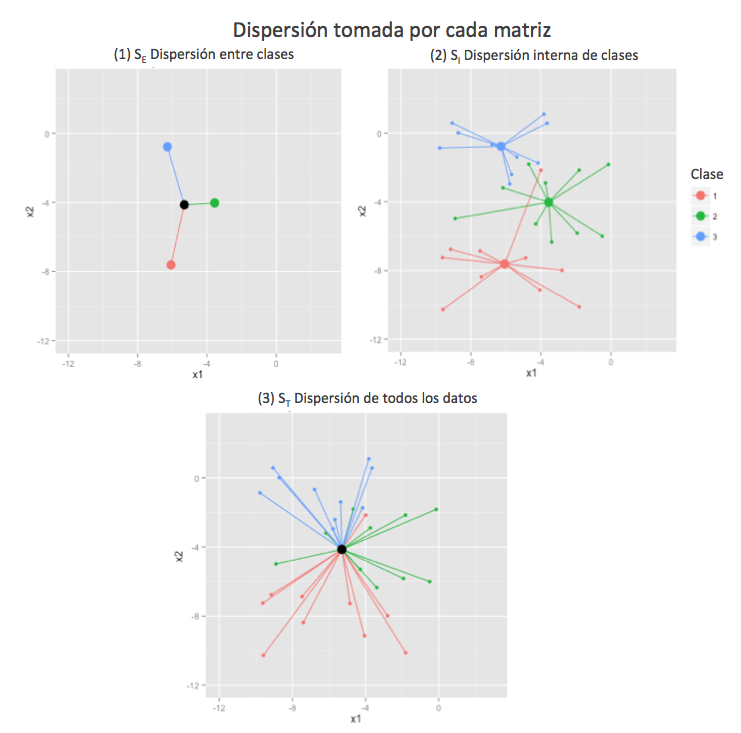
\includegraphics[width=1\textwidth]{Figures/Chapter2_SE_SI}	
  \caption[Distancias en las matrices de dispersión.]
  {En la gráfica (1) se representa la $S_E$, es decir las distancias al cuadrado entre la media de todos los datos (Punto negro) y las medias de cada clase (Puntos de color gruesos). La gráfica (2) representa $S_I$; es decir, la distancia al cuadrado de los individuos a la media de su clase. La gráfica (3) representa $S_T$, la dispersión de los datos con respecto a la media de todos.}
\end{figure}

Entre la matriz de dispersión interna $S_I$, la matriz de dispersión entre clases $S_E$ y la matriz de dispersión total $S_T$ existe una relación importante. Se cumple que $S_T = S_I + S_E $; es decir, la dispersión de las medias de grupos con la media global más la dispersión de cada clase individual es igual a la dispersión de los datos sin la información de las clases. Los datos de la figura 1.2 representan las distancias que toman en cuenta cada una de estas matrices. Para ejemplificar esta relación se generaron 10 datos por clase suponiendo distribuciones normales (El coeficiente de correlación de los datos generados es $-0.005$):

\begin{center}
\begin{tabular}{ c c c}
\toprule
\textbf{Clase} & \textbf{Distribución x1} & \textbf{Distribución x2} \\
\midrule\\
\addlinespace[-2ex]
1 & N(-5, 2.5) & N(-8, 2)\\
2 & N(-3, 2.5) & N(-4, 2)\\
3 & N(-7, 2.5) & N(-1, 2) \\
\addlinespace[1.5ex]
\bottomrule
\end{tabular}
\end{center}

Calculando las matrices de dispersión de acuerdo a las fórmulas (1.6), (1.7) y (1.8):

\begin{center}
\begin{tabular}{ c c c}
\toprule
\textbf{$S_I$} & \textbf{$S_E$} & \textbf{$S_T$} \\
\midrule\\
\addlinespace[-2ex]
$ \begin{bmatrix}  186.05 & 2.78 \\ 2.78 &  94.58 \end{bmatrix}$ &
$ \begin{bmatrix} 46.13 & -4.15 \\ -4.15 & 234.57 \end{bmatrix}$ &
$ \begin{bmatrix}  232.18 & -1.36 \\ -1.36 &  329.16 \end{bmatrix}$ \\
\addlinespace[1.5ex]
\bottomrule
\end{tabular}
\end{center}

De este ejemplo numérico se puede ver que al sumar la dispersión interna $S_I$ y la dispersión entre clases $S_E$ da como resultado la dispersión de todos los individuos $S_T$. En general este resultado se cumple, por lo que a continuación se enuncia esta relación que es muy fácil de demostrar.

\begin{proposition} \label{lemma2.1}
Sea $S_E$ la matriz de dispersión entre clases, $S_I$ la matriz de dispersión interna y $S_T$ la matriz de dispersión de los datos, entonces se tiene que cumplir la siguiente igualdad: $S_T$ = $S_I$ + $S_E$
\end{proposition}

Un problema muy común que surge en problemas de aprendizaje estadístico es que el costo computacional puede volverse intratable conforme la dimensionalidad de los individuos crece. En el ADLF se requiere hacer el cómputo de las matrices de dispersión de los individuos constantemente (o bien calcular la inversa de matrices de alta dimensionalidad), cálculos que para grandes dimensiones son sumamente costosos. Existen distintas maneras para hacer frente a este problema, uno de ellos involucra el PCA (Principal Component Analysis) en el preprocesamiento de los datos. Este método es fácil de calcular y solo requiere computar una vez la de matriz de dispersión \cite{ngo2012trace}. Debido a la finalidad de esta tesis no se profundizará en más técnicas para hacer frente a este problema, pero en textos como \cite{hastie2009elements}, \cite{duda2012pattern} aparecen distintos métodos para reducción de dimensionalidad.

Retomando el problema de cociente de trazas, lo que se busca es encontrar la proyección que mantenga juntos individuos de una clase al mismo tiempo que separa las medias de distintas clases. Una vez obtenida esta proyección se puede encontrar un hiperplano separador de los datos, o bien algún criterio para asignar la clase de pertenencia. 

\pagebreak
El problema de optimización se puede plantear como:
\begin{equation}\label{eq:2.5}
	\max_{\substack{V \in {\rm I\!R}^{n \times p} \\ V^TC V = I}} \frac{Tr(V^T S_E V)}{Tr(V^T S_I V)} 	
\end{equation}

 La solución a este problema no tiene una forma cerrada, por lo que en la literatura se buscan formulaciones alternas para resolverlo de una manera más sencilla \cite{wang2007trace} \cite{fukunaga2013introduction}, algunos ejemplos de estas formulaciones son:

\begin{equation}\label{eq:2.6}
	\max_{\substack{V \in {\rm I\!R}^{n \times p} \\ V^T S_I V = I}} Tr(V^T S_E V)
\end{equation}

\begin{equation} \label{eq:2.7}
	\max_{\substack{V \in {\rm I\!R}^{n \times p} \\ V^TC V = I}} Tr\left( \frac{V^T S_E V}{V^T S_I V}\right) 	
\end{equation}

\begin{equation} \label{eq:2.8}
	\max_{\substack{V \in {\rm I\!R}^{n \times p} \\ V^TC V = I}} \frac{|V^T S_E V|}{|V^T S_I V|} 	
\end{equation}

Con $|\bullet| = det(\bullet)$ y $Tr(\bullet) = Traza(\bullet)$.


En la siguiente parte de este capítulo se resolverá el problema original (1.9) para $p = 1$, para lo cual se introduce el cociente generalizado de Rayleigh. Para la generalización a $p$ dimensiones solo se plantea el problema y se proporcionan los casos en que la solución existe y es única. Seguido de esto se definirá una función $f(\rho)$ la cual sirve para encontrar el óptimo por métodos iterativos. Por último haciendo uso de los eigenvalores de $S_I$ y $S_E$ se darán cotas inferiores y superiores al óptimo.

\section{Problema del cociente de trazas}

El problema del cociente de trazas (Trace ratio problem) es fácil de ver cuando $V \in {\rm I\!R}^{n \times p}$ proyecta a un espacio de pocas dimensiones. Por ejemplo, cuando $p = 2$ se desea obtener la mejor proyección sobre un plano y cuando $p = 1$ sobre una recta. Para ejemplificar esta situación se creo un conjunto sintético donde cada $x_i \in {\rm I\!R}^{3}$. Las distribuciones son normales y se proyectan en ${\rm I\!R}^{2}$ y ${\rm I\!R}^{1}$. Los datos se pueden observar en la figura 1.3.

\begin{figure}[!ht]\label{Fig1.2}
  \centering
  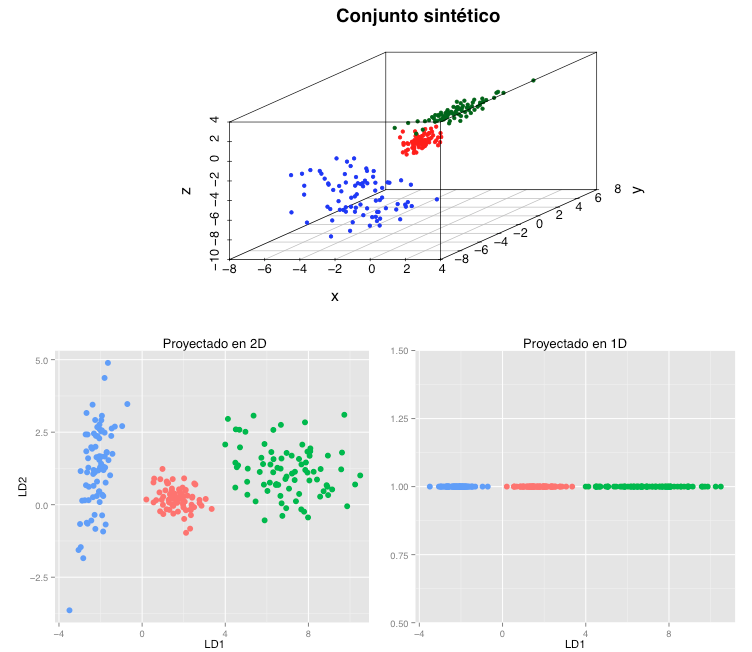
\includegraphics[width=1\textwidth]{Figures/Chapter2_1} 
  \caption[Mejores proyecciones en ${\rm I\!R}^{2}$ y ${\rm I\!R}$.]
  {En la gráfica de arriba se muestran los datos originales en 
   ${\rm I\!R}^{3}$ los cuales fueron generados a través de distribuciones normales con distintas medias y varianzas. En la gráfica de abajo a la izquierda se muestra la mejor proyección en ${\rm I\!R}^{2}$ y abajo a la derecha la mejor proyección en ${\rm I\!R}$}
\end{figure}

\subsection{Solución cuando p = 1}

El problema (1.9) toma la siguiente forma cuando $V \in {\rm I\!R}^{n}$. Se nombrara $v$ a este proyector de una dimensión ya que resulta ser solo un vector:


\begin{equation} \label{eq:2.9}
\max_{v \in {\rm I\!R}^{n}} \frac{v^T S_E v}{v^T S_I v}  
\end{equation}

Se tiene que $x_i \in {\rm I\!R}^{n}$ son los individuos originales con $i = 1 , ... , N $. Entonces sean $w_i \in {\rm I\!R}$ los individuos proyectados por el vector $v$ de manera que $w_i = v^Tx_i$. De esta manera es conveniente definir $\widehat{\mu}_k = v^T \mu_k$ y $\widehat{\mu} = v^T \mu$ como la media por clase y la media total de los datos proyectados.

\textbf{Matriz de dispersión entre clases $\Phi_{E}$ de los individuos proyectados $w_i$:}

$$\Phi_{E} = \sum\limits_{k =1}^{K} N_k (\widehat{\mu}_k - \widehat{\mu} )^2$$

$$\Phi_{E} = \sum\limits_{k =1}^{K} N_k (v^T \mu_k - v^T \mu)^2$$

$$\Phi_{E} =  \sum\limits_{k =1}^{K} N_k v^T ( \mu_k - \mu )(\mu_k - \mu )^T v $$
Por distributividad en matrices se cumple que $vAv+vBv =  v(A+B)v$, entonces:

\begin{equation}\label{eq:2.10}
\Phi_{E} = v^T \big[ \sum\limits_{k =1}^{K} N_k ( \mu_k - \mu )(\mu_k - \mu )^T \big] v	
\end{equation}

\textbf{Matriz de dispersión intra clase $\Phi_{I}$ de los individuos proyectados $w_i$}:
$$\Phi_{I} = \sum\limits_{k = 1}^{K} \sum\limits_{\substack{i = 1\\
                            y_i = k}}^{N} (w_i - \widehat{\mu}_k)^2 $$

$$\Phi_{I} = \sum\limits_{k = 1}^{K} \sum\limits_{\substack{i = 1\\
                            y_i = k}}^{N} (v_i^T x_i - v_i^T \mu_k)^{2} $$
$$\Phi_{I} =  \sum\limits_{k = 1}^{K} \sum\limits_{\substack{i = 1\\
                            y_i = k}}^{ N} v^T( x_i - \mu_k) ( x_i - \mu_k)^T v  $$

Usando de nuevo la distibutividad de matrices:

\begin{equation}\label{eq:2.11}
\Phi_{I} = v^T \big[ \sum\limits_{k = 1}^{K} \sum\limits_{\substack{i = 1\\
                            y_i = k}}^{ N} ( x_i - \mu_k) ( x_i - \mu_k)^T \big] v	
\end{equation}


 Las fórmulas de $\Phi_{I}$ y $\Phi_{E}$ de los individuos $w_i$ se pueden expresar en función de las matrices de dispersión intra clase y entre clases $S_I$ y $S_E$ de los individuos originales $x_i$. De esta manera:

 $$\Phi_{E} = f(S_E) = v^T S_E v$$
 $$\Phi_{I} = f(S_I) = v^T S_I v$$

Se tiene que $\Phi_{I}, \Phi_{E} \in {\rm I\!R}$, entonces maximizar el cociente $\frac{\Phi_{E}}{\Phi_{I}}$ con respecto a $v$ tiene como resultado una proyección que conserva cerca a los individuos pertenecientes a la misma clase, mientras que aleja a los centros de cada clase. Para el caso de una dimensión se puede encontrar una solución cerrada. La teoría asociada a este problema de maximización esta relacionada con el Cociente Generalizado de Rayleigh, el cual bajo las condiciones enunciadas de este caso, se puede transformar a un Cociente de Rayleight. Usando la proposición 1.2 se puede obtener la solución a este último.

\begin{proposition} \label{lemma2.2}
La solución a la maximización del Cociente de Rayleigh:
$$\max_{v \in {\rm I\!R}^{n} } \frac{v^T A v}{v^Tv} $$
cuando $A$ es simétrica, es obtenida cuando $v$ es el eigenvector asociado al eigenvalor más grande de la matriz $A$.
\end{proposition}


\subsection{Generalización a p dimensiones}

Para dimensiones más grandes de $v$, el Cociente Generalizado de Rayleigh no puede ser escrito en general como el Cociente de Rayleigh, por lo que la solución planteada en el capítulo anterior no es de utilidad. Esto genera la dificultad de no tener una solución cerrada, por lo que se han propuesto métodos iterativos y planteamientos alternos a la solución.

La generalización a $p$ dimensiones implica que los individuos $x_i \in {\rm I\!R}^{n}$ son proyectados ahora por la matriz $V = (V_1 | V_2 | ... |V_p)$, de manera que $w_i = V^T x_i$ con $w_i \in {\rm I\!R}^{p}$ y $V_j \in {\rm I\!R}^{n}$. De esta manera las matrices $\Phi_I$ y $\Phi_E$ se definen como sigue:

\begin{equation*}
\Phi_E = \sum\limits_{k = 1}^{K} N_{k} ||\widehat{\mu}_k - \widehat{\mu}||_2^2
\end{equation*}

\begin{equation*}
\Phi_E = \sum\limits_{k = 1}^{K} N_{k} ||V^T \mu_k - V^T \mu||_2^2
\end{equation*}

\begin{equation*}
\Phi_E = \sum\limits_{k = 1}^{K} N_{k} ||V^T (\mu_k - \mu)||_2^2
\end{equation*}


\begin{equation}\label{eq:2.17}
  \Phi_E = \sum\limits_{k = 1}^{K} N_{k} \big[ (V_1^T (\mu_k - \mu))^2 + (V_2^T (\mu_k - \mu))^2+ ... + (V_p^T (\mu_k - \mu))^2 \big]
\end{equation}

De esta expresión hay que destacar que $V_1^T (\mu_k - \mu)$ es un escalar, ya que $V_1 \in {\rm I\!R}^n$ y $(\mu_k - \mu) \in {\rm I\!R}^{n}$. Otra fórmula equivalente y que es comúnmente usada por sus propiedades algebraicas consiste en la siguiente expresión:

\begin{equation}\label{eq:2.18}
\Phi_E = \sum\limits_{k = 1}^{K} N_{k} Tr \big[ V^T (\mu_k - \mu) (\mu_k - \mu)^T V \big]	
\end{equation}

Para ejemplificarla se toma una clase $k = k_1$.  Al desarrollar $(\bullet) = V^T (\mu_1 - \mu) (\mu_1 - \mu)^T V$ se tiene una matriz en ${\rm I\!R}^{p \times p}$ igual a:


\begin{equation*}
(\bullet)= \left(\!
    \begin{array}{c}
      V_1^T (\mu_1-\mu)\\
      V_2^T (\mu_1-\mu)\\
      \vdots \\
      V_p^T (\mu_1-\mu)
    \end{array}
  \!\right) 
  \left(\!\begin{array}{c}
      (\mu_1-\mu)^T V_1 \quad
      (\mu_1-\mu)^T V_2 \quad
      \hdots \quad
      (\mu_1-\mu)^T V_p
    \end{array}
  \!\right) 
\end{equation*} 

\vspace{5mm}

\begin{equation*}
(\bullet)= \left(\!
    \begin{array}{ccc}
      V_1^T (\mu_1-\mu) (\mu_1-\mu)^T V_1 & \hdots & V_1^T (\mu_1-\mu) (\mu_1-\mu)^T V_p  \\
      V_2^T (\mu_1-\mu) (\mu_1-\mu)^T V_1 & \hdots & V_2^T (\mu_1-\mu) (\mu_1-\mu)^T V_p  \\
      \vdots & \ddots & \vdots\\
      V_p^T (\mu_1-\mu) (\mu_1-\mu)^T V_1 & \hdots & V_p^T (\mu_1-\mu) (\mu_1-\mu)^T V_p
    \end{array}
  \!\right) 
\end{equation*} 

\vspace{5mm}

\begin{equation*}
(\bullet)= \left(\!
    \begin{array}{ccc}
      (V_1^T (\mu_1-\mu))^2 & \hdots & V_1^T (\mu_1-\mu) (\mu_1-\mu)^T V_p \\
       V_2^T (\mu_1-\mu) (\mu_1-\mu)^T V_1  & \hdots & V_2^T (\mu_1-\mu) (\mu_1-\mu)^T V_p  \\
      \vdots & \ddots & \vdots\\
      V_p^T (\mu_1-\mu) (\mu_1-\mu)^T V_1  & \hdots & (V_p^T (\mu_1-\mu))^2
    \end{array}
  \!\right) 
\end{equation*} 

\vspace{5mm}

 Por lo tanto al calcular la traza de la matriz de $p \times p$ desarrollada arriba, se tiene que $Tr(V^T (\mu_1 - \mu) (\mu_1 - \mu)^T V)$ es equivalente a:
 \vspace{3mm}
 \begin{equation*}
Tr(\bullet) = (V_1^T (\mu_1-\mu))^2+ (V_2^T (\mu_1-\mu) )^2 + \hdots + (V_p^T (\mu_1-\mu) )^2
 \end{equation*}

Al generalizar a las $K$ clases y usando la propiedad de linealidad en la traza; es decir, $Tr(A+B) = Tr(A)+Tr(B)$, entonces se puede escribir de la siguiente manera:

\begin{equation*}
\Phi_E = Tr \sum\limits_{k = 1}^{K} N_{k}  \big[ V^T (\mu_k - \mu) (\mu_k - \mu)^T V \big]
\end{equation*}


Esta expresión es equivalente a (1.16). Como paso final se factoriza $V^T$ y $V$ sobre todos los sumandos, lo que nos llevaría a lo siguiente:

\begin{equation*} 
\Phi_E =  Tr (V^T \sum\limits_{k = 1}^{K} N_{k}  \big[(\mu_k - \mu) (\mu_k - \mu)^T \big] V)   
\end{equation*}

o, expresada en términos de $S_E = \sum\limits_{k = 1}^{K} N_{k}  \big[(\mu_k - \mu) (\mu_k - \mu)^T \big]$

\begin{equation}\label{eq:2.19}
\Phi_E =  Tr (V^T S_E V)     
\end{equation}

Similarmente se puede llegar a la formulación de la varianza intra-clase $\Phi_{I}$.
\begin{equation}\label{eq:2.20}
\Phi_{I} =  Tr (V^T S_I V )
\end{equation}



\subsection{Existencia de la solución}

Para demostrar la existencia y unicidad de la solución, las matrices $S_I$ y $S_E$ deben cumplir ciertas características. Sean $A = S_E$ y $B = S_I$, la primer condición que se les impone es que sean positivas definidas. La razón que apoya la restricción está relacionada con la forma de la función a maximizar, que es un cociente. Como $B$ se encuentra en el denominador, se tiene que evitar que $Tr(V^T B V) = 0$, ya que con este valor se indetermina la función objetivo \cite{ngo2012trace}. 

T.T. Ngo propone generalizar el estudio a las matrices positivas semidefinidas. Para esto se deben encontrar los casos en que $Tr(V^T B V)$ toma el valor de $0$. Si se diagonaliza a la matriz $B = Q \Lambda_{B} Q^T$ con $Q$ ortogonal y $\Lambda_{B}$ una matriz diagonal con entradas iguales a los eigenvalores de $B$, entonces:

\begin{equation*}
Tr(\Lambda_{B}) = \lambda_{B_1}+ \lambda_{B_2}+ ... +\lambda_{B_n} \qquad con \qquad \widehat{V} = Q^T V
\end{equation*}



De este modo $\widehat{V} = (\widehat{V}_1 | \widehat{V}_2 | ... | \widehat{V}_p)$ y cada $\widehat{V}_i^T = (\widehat{V}_{i1}, \widehat{V}_{i2}, ..., \widehat{V}_{in})$ es un vector renglón. De esta manera la matriz $\widehat{V}^T$:

\begin{equation*}
\widehat{V}^T = 	
\left(\!
    \begin{array}{c}
      \widehat{V}_1^T\\
      \widehat{V}_2^T\\
      \vdots \\
      \widehat{V}_p^T
    \end{array}
  \!\right)   = 
\left(\!
    \begin{array}{cccc}
      \widehat{V}_{11} & \widehat{V}_{12} & \hdots & \widehat{V}_{1n}\\
      \widehat{V}_{21} & \widehat{V}_{22} & \hdots & \widehat{V}_{2n}\\
      \vdots &  \vdots &\ddots & \vdots\\
      \widehat{V}_{p1} & \widehat{V}_{p2} & \hdots & \widehat{V}_{pn}\\
    \end{array}
  \!\right) 
\end{equation*}

Por lo que la traza que involucra a $B$ tiene la siguiente forma:

\begin{equation*}
Tr(V^T B V) = Tr(V^T Q \Lambda_{B} Q^T V) 	
\end{equation*}

\begin{equation*}
Tr(V^T B V)  = Tr(\widehat{V}^T \Lambda_{B} \widehat{V})
\end{equation*}

\begin{equation*}
V^T B V = 
\left(\!
    \begin{array}{c}
      \widehat{V}_1^T\\
      \widehat{V}_2^T\\
      \vdots \\
      \widehat{V}_p^T
    \end{array}
  \!\right) 
  \left(\!
    \begin{array}{cccc}
      \lambda_{B_1} & 0 & \hdots & 0\\
      0 & \lambda_{B_2} & \hdots & 0\\
      \vdots &  \vdots &\ddots & \vdots\\
      0 & 0 & \hdots & \lambda_{B_n}\\
    \end{array}
  \!\right) 
  \left(\!\begin{array}{c}
      \widehat{V}_1 |
      \widehat{V}_2 |
      \hdots |
      \widehat{V}_p
    \end{array}
  \!\right) 
\end{equation*} 

Desarrollando la multiplicación de matrices, y calculando la traza resulta en los siguientes sumandos:
 
 \begin{equation*}
\begin{aligned}
      Tr(V^T B V) =& \lambda_{B_1} \widehat{V}_{11}^2&  +
                     & \lambda_{B_2} \widehat{V}_{12}^2& +
                     & \hdots& +
                     &\lambda_{B_n} \widehat{V}_{1n}^2& + \\
                     & \lambda_{B_1} \widehat{V}_{21}^2&+
                     & \lambda_{B_2} \widehat{V}_{22}^2& +
                     & \hdots& +
                     &\lambda_{B_n} \widehat{V}_{2n}^2& + \\
                     & \vdots&  
                     & \vdots& 
                     & \vdots& 
                     & \vdots& \\
                     & \lambda_{B_1} \widehat{V}_{p1}^2&+
                     & \lambda_{B_2} \widehat{V}_{p2}^2& +
                     & \hdots& + 
                     & \lambda_{B_n} \widehat{V}_{pn}^2.&  
 \end{aligned}
 \end{equation*}

 Es fácil de ver que la expresión de arriba tiene $p \times n$ sumandos, por lo que se puede expresar en términos de dos sumatorias. La primera de $j=1,...,p$ y la segunda de $i = 1,...n$:

\begin{equation*} 
Tr(V^T B V) = \sum \limits_{j=1}^{p} \sum\limits_{i=1}^{n} \lambda_{B_i} \widehat{V}_{ji}^2
\end{equation*}

\begin{equation}\label{eq:2.21}
Tr(V^T B V) = \sum\limits_{i=1}^{n} \lambda_{B_i} \sum \limits_{j=1}^{p} \widehat{V}_{ji}^2    
\end{equation}

De la última expresión se separa la sumatoria sobre $i$. De esta manera, para cada elemento $i$ se tienen dos factores:

\begin{equation}\label{eq:2.22}
(i) \lambda_{B_i}
\end{equation}

 \begin{equation}\label{eq:2.23}
 (ii) \sum \limits_{j=1}^{p} \widehat{V}_{ji}^2   
 \end{equation}
 

 La idea para que $Tr(V^T B V)$ sea positivo, es que al menos uno de los sumandos sea positivo. Si (1.21) y (1.22) son ambos distintos de cero para al menos una $i$, entonces se cumple esta condición. Esta idea está expresada en el Lema 1.1.

\begin{lemma}\label{lemma2.4}
Sea $B$ positiva semidefinida y $V \in {\rm I\!R}^{n\times p}$. Si $B$ tiene a lo más $p-1$ eigenvalores iguales a $0$, entonces $Tr(V^T B V)  = Tr(\widehat{V}^T \Lambda_{B} \widehat{V}) \neq 0$  para cualquier matriz ortogonal $V$.
\end{lemma}

\begin{proof}
Sea $\widehat{V} = [\widehat{V}_1 | ... | \widehat{V}_p]$ tal que $\widehat{V} \widehat{V} = V^T Q Q^T V = V^T I_n V  = I_p$. De esta manera se puede construir una matriz $\widehat{V}' \in {\rm I\!R}^{p \times p}$ seleccionando $p$ de los $n$ renglones de $\widehat{V}$ tal que $\widehat{V}'$ sea no singular. $\widehat{V}'$ tiene la propiedad de no contener eigenvalores iguales a 0; como consecuencia, sus renglones y columnas no contienen al vector $\widehat{0}$. Al no contenerlo,se sabe que al menos hay $p$ renglones de $\widehat{V}$ tal que $\sum_{j=1}^{p}\widehat{V}_{ji}^2 \neq 0$ para cada uno de ellos. Por otra parte en el lema se supone que la matriz $B$ tiene a lo más $p-1$ eigenvalores iguales $0$ por lo que al menos un elemento de la sumatoria es distinto de cero.
\end{proof}

Analizando a mayor profundidad el resultado anterior, se sabe que hay $n-p+1$ eigenvalores de $B$ positivos ($\lambda_{B_i} \neq 0$) y $p$ renglones de $\widehat{V}$ que tienen norma distinta de cero. Al calcular la sumatoria (1.20), se tiene que al menos una combinación de $\lambda_{B_i}$ y uno de los $p$ renglones cumplen que su multiplicación tiene signo positivo. Para ejemplificar esta situación sean $C_i$ con $i = 1, ... , n-p+1$ los eigenvalores de $B$ y $K_j$ con $j = 1, ... , p$ la norma de los renglones de $\widehat{V}$ que son distintos de $0$.
 
\begin{center}
\begin{tabular}{ | c | c|  c | c|} 
\hline
$i$ & $\lambda_{B_i}$ & $\sum \limits_{j=1}^{p} \widehat{V}_{ji}^2$  & $\lambda_{B_i} \sum \limits_{j=1}^{p} \widehat{V}_{ji}^2$ \\ 
\hline
\hline
1 & $C_1$ & $0$ & $0$ \\ 
\hline
2 & $C_2$ & $0$ & $0$ \\ 
\hline
\vdots & \vdots & \vdots & \vdots \\ 
\hline
$n-p$ & $C_{n-p}$ & $0$ &  $0$\\ 
\hline
$n-p+1$ & $C_{n-p+1}$ & $K_{p}$ &  $C_{n-p+1} K_{p}$\\ 
\hline
$n-p+2$ & $0$ & $K_{p-1}$  & $0$ \\ 
\hline
\vdots & \vdots & \vdots & \vdots  \\ 
\hline
$n-1$ & $0$ & $K_2$ & $0$ \\ 
\hline
$n$ & $0$ & $K_1$ & $0$ \\ 
\hline
\hline

\end{tabular}
\end{center}

Con esta combinación se tiene que al menos hay un sumando de $\sum\limits_{i=1}^{n} \lambda_{B_i} \sum \limits_{j=1}^{p} \widehat{V}_{ji}^2 $ distinto de cero, por lo que $Tr(V^T B V) \neq 0$. Bajo estas condiciones se garantiza que el denominador sea mayor a 0, solo falta asegurarse que el numerador sea menor a infinito.

\begin{lemma}
Sea $U_p = \{ V \in {\rm I\!R}^{n \times p} | V^T V = I_p \} $ un conjunto compacto con $V = (v_1, v_2, ... , v_p)$
\end{lemma}
\begin{proof}
Se tiene que $U_p$ es un conjunto cerrado porque contiene a todos sus puntos límite; por otro lado, $U_p$ también es acotado bajo la norma 2 y la norma de Frobenius:

Tomando la norma-2 y la norma de Frobenius de $V$: 
\begin{equation*}
\begin{aligned}
	||V||_2 =& Max \{||V_x ||_2 \quad | \quad ||x||_2 = 1 \} \\
		    =& ||V_x||^2_2  \\
		    =& (Vx)^T (Vx) \\
		    =& x^T V^T V x\\
		    =& x^T x = 1\\
	||V||_F	=& \sum\limits_{F}^{p} ||v_i|| = p   
\end{aligned}
\end{equation*}

Entonces se tiene $U_p$ es cerrado y acotado, por lo que $U_p$ es compacto.
\end{proof}

Con este resultado se tiene que $Tr(V^T A V)$ toma un valor finito ya que todas sus entradas son finitas. 


\begin{lemma}\label{lemma2.5}
Sean $A$ y $B$ dos matrices simétricas tales que $B$ es positiva semidefinida con rango mayor que $n-p$; es decir, que tenga al menos $n-p+1$ eigenvalores distintos de cero. Entonces el cociente $(1.9)$ admite un máximo con valor $\rho^*$ \cite{ngo2012trace}.
\end{lemma}

\begin{proof}
Tomando el resultado del lema 1.1 se tiene que $Tr(V^T B V) \neq 0$; por otra parte, $V \in U_p$ que es un conjunto compacto. Con estas dos observaciones, el valor de (1.9) es distinto de infinito. Entonces el cociente $(1.9)$ admite un máximo con valor $\rho^*$ y que tiene como argumento $V^{**}$.
\end{proof}

\subsection{Equivalencia con un problema escalar}

\textbf{Valor en el óptimo}. Del lema 1.3 se sabe que existe una matriz $V^{**} \in U_p$ tal que (1.9) alcanza el valor máximo $\rho^*$. Expresando esta idea se tiene que:

\begin{equation} \label{eq:2.24}
 \frac{Tr(V^{T**} A V^{**})}{Tr(V^{T**} B V^{**})} = \rho^* 
\end{equation}

Entonces para cualquier otra matriz $V \in U_p $:

\begin{equation}\label{eq:2.25}
 \frac{Tr(V^T A V)}{Tr(V^T B V)} \leq \rho^* 
\end{equation}

Como la traza es un operador lineal y por la propiedad distributiva de las matrices entonces (1.24) es equivalente a:

\begin{equation*}
 Tr(V^T A V)- \rho^* Tr(V^T B V) \leq 0 
\end{equation*}

\begin{equation*}
	Tr(V^T A V- \rho^* V^T B V) \leq 0	
 \end{equation*}

 \begin{equation} \label{eq:2.26}
	Tr(V^T (A - \rho^* B )V) \leq 0	
 \end{equation}

y el resultado equivalente para (1.23):
	
 \begin{equation} \label{eq:2.27}
	Tr(V^{T**} (A - \rho^* B )V^{**}) = 0	
 \end{equation}


Para facilitar la lectura, de aquí en adelante se define la función $G(\rho) = A- \rho B$. Maximizar el lado izquierdo de la desigualdad (1.25) sujeto a $V^T V = I$ es equivalente a maximizar un problema de eigenvalores generalizado. Usando lo establecido en el apéndice A, se sabe que el valor máximo de este problema dado $\rho^*$:

\begin{equation}\label{eq:2.28}
	\max_{\substack{V \in {\rm I\!R}^{n \times p} \\ V^T V = I}} Tr(V^T G(\rho^*) V) = \lambda_{G(\rho^*)_1} + \lambda_{G(\rho^*)_2} + ... + \lambda_{G(\rho^*)_p}
\end{equation}
  
 Con $\lambda_{G(\rho^*)_1} \geq \lambda_{G(\rho^*)_2} \geq ... \geq \lambda_{G(\rho^*)_p}$ los $p$ eigenvalores más grandes de $G(\rho^*)$. De esta manera el valor óptimo de (1.27) es simplemente la suma de los $p$ eigenvalores más grandes de esta matriz, y $V^{**}$ el conjunto de correspondientes eigenvectores. Para obtener este valor y la matriz, el primer paso es encontrar a $\rho^*$, ya que teniéndolo es inmediato calcular $V^{**}$. Dada esta premisa, se puede ver que el problema a resolver se reduce a buscar el valor óptimo de $\rho$. Para esto se define la función $f(\rho)$ sobre todo $\rm I\!R$, tal que $f(\rho)$ es continua sobre su argumento $\rho$: 

\begin{equation}  \label{eq:2.29}
	f(\rho) = \max_{V^T V = I} Tr(V^T (G(\rho)) V)
\end{equation}

Es conveniente examinar $f(\rho)$ con dos objetivos, el primero es estimar la dificultad de calcular el valor de $f(\rho)$ y el segundo es encontrar la maximización adecuada para obtener $\rho^*$. Respecto al primer punto, la manera de calcular $f(\rho)$ en cada punto es equivalente a (1.27), pero en lugar de usar los eigenvalores de $G(\rho^*)$ se usan los de $G(\rho)$. En particular se llamará $V(\rho)^*$ al argumento que resuelve (1.28) \footnote{Se utilizó la nomenclatura de $V(\rho^*)$ porque estos eigenvectores dependen del valor de $\rho$ en la matriz $A - \rho B$.}. Sean $\lambda_{G(\rho)_1} \geq \lambda_{G(\rho)_2} \geq ... \geq \lambda_{G(\rho)_n}$ los $n$ eigenvalores de $G(\rho)$. Con esta notación $f(\rho)$ toma el valor de:


\begin{equation}\label{eq:2.30}
f(\rho) = \lambda_{G(\rho)_1} + \lambda_{G(\rho)_2} + ... +\lambda_{G(\rho)_p}
\end{equation}


Para el segundo punto, la idea es iterar hasta obtener el valor de $\rho^*$. Por esto, es conveniente analizar como se comporta la función con respecto a su argumento. A continuación se presentan dos propiedades de $f(\rho)$. Para demostrarlas, primero se enuncia el teorema 8.1.5 de \cite{golub2012matrix}.

\begin{theorem} \label{teorem.1}
	
	Sean $X$ y $X+E$ matrices simétricas $n \times n$, y $\lambda_{X_k}$, $\lambda_{E_k}$ los k-ésimos eigenvalores más grandes de $X$ y $E$ respectivamente. De esta manera $\lambda_{X_k}$ es el k-ésimo eigenvalor más grande de $X$ y $\lambda_{E_1}$ el más grande de $E$. Con estas definiciones se cumple lo siguiente:

	\begin{equation}\label{eq:2.31}
		\lambda_{X_k} +\lambda_{E_n} \leq \lambda_{(X+E)_k} \leq \lambda_{X_k} +\lambda_{E_1}
	\end{equation}

\end{theorem}

Se procede a enunciar este lema acerca de la función $f(\rho)$

\begin{lemma}\label{lemma2.6}
La función $f(\rho) = \max_{V^T V = I} Tr(V^T (A - \rho B) V)$ cumple las siguientes dos propiedades: 

(1) $f$ es una función no creciente de $\rho$ \\
(2) $f(\rho)= 0$  si y solo si $\rho = \rho^*$
\end{lemma}

Para probar la parte $(1)$ del lema 1.4 se comparan los valores de $f(\rho)$ para $\rho_1$ y $\rho_2$ con $\rho_2 \geq \rho_1$. Como se desea demostrar que $f$ es una función no creciente de $\rho$, se busca que $f(\rho_2) \leq f(\rho_1)$. Se definen las matrices $Y=X+E$ y $E = Y-X$, para después restarles $\lambda_{X_k}$, entonces (1.29) se puede escribir como:

\begin{equation*}
		\lambda_{(X)_k} +\lambda_{(Y-X)_n} \leq \lambda_{(Y)_k} \leq \lambda_{(X)_k} +\lambda_{(Y-X)_1}
\end{equation*}

\begin{equation*}
		\lambda_{(Y-X)_n} \leq \lambda_{(Y)_k} - \lambda_{(X)_k} \leq \lambda_{(Y-X)_1}
\end{equation*}

La expresión en el centro de estas desigualdades es la resta del eigenvalor k-ésimo de la matriz $X$ y $Y$, por lo que si se realiza la suma de $k = 1$ a $k = p$ se tiene lo siguiente:

\begin{equation}\label{eq:2.32}
		p \lambda_{(Y-X)_n} \leq \sum_{k=1}^{p} \lambda_{(Y)_k} - \sum_{k=1}^{p} \lambda_{(X)_k} \leq  p \lambda_{(Y-X)_1}
\end{equation}

Definiendo $X = A - \rho_2 B$ y $Y = A - \rho_1 B$, entonces (1.31) toma la siguiente forma:

\begin{equation}\label{eq:2.33}
    p \lambda_{(B(\rho_2-\rho_1))_n} \leq \sum_{k=1}^{p} \lambda_{(A - \rho_1 B)_k} - \sum_{k=1}^{p} \lambda_{(A - \rho_2 B)_k} \leq  p \lambda_{(B(\rho_2-\rho_1))_1}
\end{equation}

Retomando el resultado (1.29), y sustituyéndolo en (1.32) la desigualdad queda de la siguiente forma:

\begin{equation}\label{eq:2.34}
		p \lambda_{(B (\rho_2 - \rho_1))_n} \leq f(\rho_1) - f(\rho_2) \leq  p \lambda_{(B (\rho_2 - \rho_1))_1}
\end{equation}


En la parte izquierda de la desigualdad anterior, se puede a determinar el signo que toman los eigenvalores $\lambda_{(B (\rho_2 - \rho_1))_n}$. 
Si $(\rho_2- \rho_1) \geq 0$ entonces la matriz $(\rho_2 - \rho_1)B$ es positiva semidefinida; por lo tanto, todos sus eigenvalores son mayores o iguales a 0:

\begin{equation*}
	0 \leq p \lambda_{(B (\rho_2 - \rho_1))_n} \leq f(\rho_1) - f(\rho_2) \leq  p \lambda_{(B (\rho_2 - \rho_1))_1}
\end{equation*}
	
\begin{equation}\label{eq:2.35}
	0 \leq f(\rho_1) - f(\rho_2)
\end{equation}

De esta manera $f(\rho_2)  \leq  f(\rho_1) $ cuando $\rho_2 \geq \rho_1$

Para probar la parte (2) del lema 1.4, se tiene que demostrar la condición suficiente y la condición necesaria. La demostración de la primera es inmediata, ya que cuando $\rho = \rho^*$, entonces por (1.26), $f(\rho) = 0$. Para la condición necesaria se usará (1.23) y la propiedad que la $Tr(V^T B V) >0 \enspace \forall \enspace V \in U_p$. Se demostrará que, dado $f(\rho^*) = 0$, entonces:


\begin{equation}\label{eq:2.36}
	(i) \quad f(\rho) < 0 \quad si \quad \rho>\rho^*
\end{equation}
\begin{equation}\label{eq:2.37}
	(ii) \quad f(\rho) > 0 \quad si \quad \rho<\rho^*
\end{equation}

\underline{\textbf{Caso (i) $\rho > \rho^* $}}

Se tiene que las siguientes desigualdades se cumplen:
\begin{equation*}
\frac{Tr(V^T A V)}{Tr(V^T B V)} \leq \rho^* < \rho	
\end{equation*}

Por lo que es equivalente a:

\begin{equation*}
	Tr(V^T (A -\rho B)V) < 0 \quad \forall V \in U_p
\end{equation*}


De esta manera $f(\rho) < 0$ cuando $\rho > \rho^*$.
\vspace{5mm}

\underline{\textbf{(ii) $\rho < \rho^* $}}

Retomando el resultado (1.24) y suponiendo que $\rho^* > \rho$ entonces existe una $V^{*}$ tal que:


 \begin{equation*} 
 \rho < \frac{Tr(V^{T*} A V^*)}{Tr(V^{T*} B V^*)} \leq \rho^*
 \end{equation*}

\begin{equation*}
Tr(V^{T*} A V^* - \rho V^{T*} B V^*) > 0 \quad \Longrightarrow \quad \frac{Tr(V^{T*} A V^*)}{Tr(V^{T*} B V^{*})} > \rho
\end{equation*}

En particular:

\begin{equation*}
\max_{V^TV} \frac{Tr(V^{T} A V)}{Tr(V^{T} B V)} > \rho
\end{equation*}

De esta manera $f(\rho) > 0$ cuando $\rho < \rho^*$.


Las ecuaciones (1.35) (1.36), junto con la continuidad de la funcion $f$, muestran que $f(\rho) = 0$ implica $\rho = \rho^*$ \cite{ngo2012trace}. De esta manera el problema puede ser visto como encontrar la raíz de la función $f(\rho)$. La figura 1.4 muestra como es esta función.

\begin{corollary}
La función $f(\rho) = \max_{V^TV = I} Tr(V^T (A -\rho B)V)$ cumple las siguientes condiciones:

$$f(\rho) > 0  \quad \forall \quad \rho \in (-\inf, \rho^*)$$
$$f(\rho) < 0  \quad \forall \quad \rho \in (\rho^*, \inf)$$

\end{corollary}

\begin{figure}[!ht]\label{Fig1.3}
  \centering
	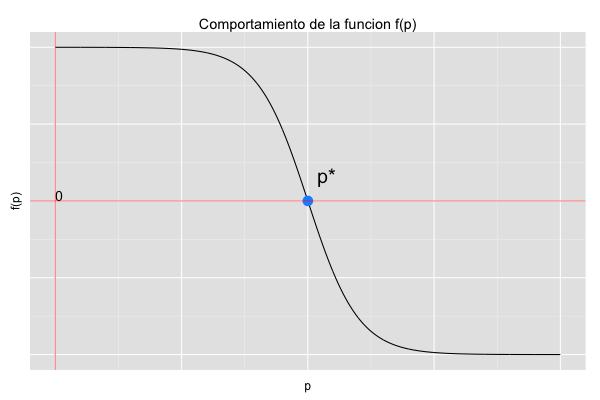
\includegraphics[width=1\textwidth]{Figures/Chapter2_fp}	
  \caption[Comportamiento de $f(\rho)$.]
  {La función $f(\rho)$ es no creciente para toda $\rho$. El valor de $f(\rho) = \lambda_{G(\rho)1}+ \lambda_{G(\rho)2} + ... +\lambda_{G(\rho)p}.$ $f(\rho^*) = 0 $}
\end{figure}


\begin{example} \label{ex:1}
Para ejemplificar el lema 1.4 se muestran las matrices $A,B \in {\rm I\!R}^{3 \times 3}$. Para el valor de $f(\rho)$ se utiliza la propiedad (1.29):

$$f(\rho) = \lambda_{G(\rho)1} + \lambda_{G(\rho)2} + ... + \lambda_{G(\rho)p}$$

con $p$ la dimensión a la que se va a proyectar. 


\begin{equation*}
A = \left(\!
    \begin{array}{ccc}
      4 & 0 & 0 \\
      0 & 6 & 0 \\
      0 & 0 & 8 
    \end{array}
  \!\right), \quad
B = \left(\!
    \begin{array}{ccc}
      1.5 & 0 & 0 \\
      0 & 2.5 & 0 \\
      0 & 0 & 5 
    \end{array}
\!\right) 
\end{equation*}



\begin{equation*}
G(\rho) = A- \rho B = \left(\!
    \begin{array}{ccc}
      4-1.5\rho & 0 & 0 \\
      0 & 6-2.5\rho & 0 \\
      0 & 0 & 8-5\rho 
    \end{array}   	
      \!\right) 
\end{equation*}

Los eigenvalores de esta matriz son $4-1.5\rho$,  $6-2.5\rho$ y  $8-5\rho$. Las funciones graficadas de estos eigenvalores se presentan en la figura 1.5.

\begin{figure}[!ht] \label{Fig1.4}
  \centering
  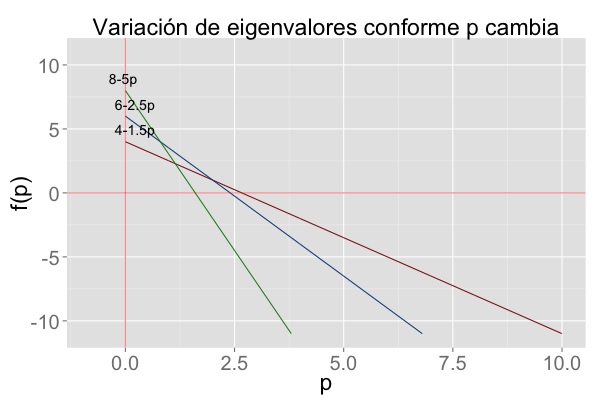
\includegraphics[width=1\textwidth]{Figures/Chapter2_3eigen}  
  \caption[Gráfica de los eigenvalores en función de $\rho$.] {Cada línea representa como se comporta cada eigenvalor de $A- \rho B$ cuando se varía $\rho$.}
\end{figure}

Cuando se desea que el proyector sea de dimensión 1, entonces se tiene que $f(\rho)$ es el eigenvalor más grande,  cuando sea de dimensión 2, la suma de los dos más grandes y así respectivamente. El valor de $f(\rho)$ para estos tres casos está representado en la figura 1.5.

\begin{figure}[!ht] \label{Fig1.5}
  \centering
  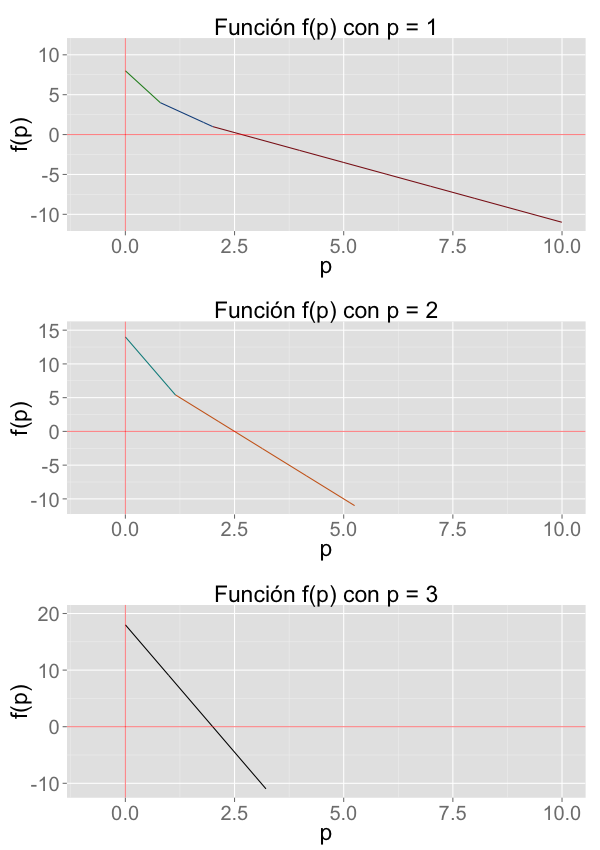
\includegraphics[width=1\textwidth]{Figures/Chapter2_grid3eigen}  
  \caption[$f(\rho)$ para proyectores de 1,2 y 3 dimensiones.] {La figura superior representa a $f(\rho) = \lambda_{G(\rho)_1}$, la de enmedio $f(\rho) = \lambda_{G(\rho)_1} + \lambda_{G(\rho)_2}$ y la de abajo $f(\rho) = \lambda_{G(\rho)_1} + \lambda_{G(\rho)_2} + \lambda_{G(\rho)_3}$.}
\end{figure}

\end{example}
\pagebreak

\subsection{Localización del óptimo}

En la sección anterior se encontró que la maximización al cociente de trazas puede ser visto como el problema de encontrar la raíz de la función $f(\rho) = max_{V^T V= I} Tr(V^T(A-\rho B)V)$. Por esto, encontrar un intervalo $(\rho_1, \rho_2)$ que contenga al valor óptimo $\rho^*$ puede reducir el número de iteraciones del método. Usando el lema 1.4 se sabe que $f$ es una función no creciente de $\rho$. Por esta razón si se encuentra una $\rho_1$ y $\rho_2$ tal que $f(\rho_1) \geq 0$ y $f(\rho_2) \leq 0$ y con la propiedad de continuidad de la funcion $f(\rho)$ entonces se encontró un intervalo que contiene a $\rho^*$. 

En esta tesis se dan cotas para el valor de $\rho^*$, la primera en función los eigenvalores de una transformación de $B -\rho A$ y la segunda en función de los eigenvalores de $B$ y $A$ \cite{ngo2012trace}. La demostración de cada una requiere del conocimiento del concepto de inercia y del Teorema de la Inercia de Sylvester. Por este motivo se presentan a continuación: \footnote{La demostración de este teorema puede ser encontrada en \cite{golub2012matrix}.}

\begin{definition}
La inercia de una matriz simétrica $A$ es la tripleta de enteros no negativos $(m, z, p)$ donde $m$, $z$ y $p$ son respectivamente el número de eigenvalores negativos, cero y positivos de $A$ \cite{golub2012matrix}.
\end{definition}

\begin{theorem}\label{teorem.2}
Sea $A \in {\rm I\!R}^{n \times n}$ una matriz simétrica y $Z \in {\rm I\!R}^{n \times n}$ no singular. Entonces $A$ y $Z^T A Z$ tienen la misma inercia \cite{golub2012matrix}.
\end{theorem}

\begin{proposition}
La raíz $\rho^*$ de $f(\rho)$ está localizada en el intervalo $(\lambda_p, \lambda_1)$ donde $\lambda_p$ es el p-ésimo eigenvalor más grande de $Z^T(A-\rho B)Z$.
\end{proposition}

\begin{proof}
Sea $Z$ la matriz que diagonaliza a $A-\rho B$ de manera que\footnote{El cálculo de esta matriz puede obtenerse en el algoritmo 8.7.1 de \cite{golub2012matrix}}:

\begin{equation}\label{eq:2.38}
\begin{aligned}
 Z^T AZ = \Lambda \\ Z^T B Z = I
 \end{aligned}
\end{equation}

Con $\Lambda$ una matriz diagonal y $\mu_1, \ldots,  \mu_n$ sus respectivos eigenvalores e $I$ la identidad de tamaño $n$. Entonces por el teorema 1.2 se sabe que $A- \rho B$ y $Z^T(A- \rho B)Z = \Lambda -\rho I$ tienen el mismo número de eigenvalores positivos, negativos y cero. Por lo tanto, la matriz en cuestión es de la siguiente forma:

\begin{equation}\label{eq:2.39}
\Lambda - \rho I = 
\left(\!
    \begin{array}{cccc}
      \mu_1 & 0 & \hdots & 0\\
      0 & \mu_2 & \hdots & 0\\
      \vdots & \vdots & \ddots & \vdots \\
      0 & 0 & \hdots & \mu_n
    \end{array}
  \!\right) - \rho
  \left(\!
    \begin{array}{cccc}
      1 & 0 & \hdots & 0\\
      0 & 1 & \hdots & 0\\
      \vdots & \vdots & \ddots & \vdots \\
      0 & 0 & \hdots & 1
    \end{array}
  \!\right) 
\end{equation} 

Como la  matriz $V$ de (1.9) es de tamaño $n \times p$, solo nos interesa saber el signo de los $p$ eigenvalores más grandes. Tomando $\rho = \mu_p$ entonces los elementos de la diagonal de la matriz $\Lambda- \rho I$ son de la forma:


\begin{equation}\label{eq:2.40}
\begin{aligned}
   \mu_i - \mu_p & \geq 0  \quad para \quad i \geq p\\
   \mu_i - \mu_p & \leq 0  \quad para \quad i \leq p
\end{aligned}
\end{equation} 

Los primeros p elementos tienen la propiedad de ser no negativos, ya que $\lambda_{(A-\rho B)_1} \geq \lambda_{(A-\rho B)_2} \geq ... \geq \lambda_{(A-\rho B)_p}$. Usando el teorema 1.2 se sabe que los primeros p eigenvalores de $A-\rho B$ también son no negativos. Por ende la suma de ellos es mayor o igual que cero. 

Por otro lado si se toma $\rho = \mu_1$. Entonces los elementos de la diagonal de la matriz (1.38) son de la forma:

\begin{equation}\label{eq:2.41}
   \mu_i - \mu_1  \leq 0 \quad \forall \quad i
\end{equation} 

Con $i = 1, ..., p$, cada uno de los elementos de la diagonal tiene la propiedad de ser no positivo por el mismo argumento que el caso pasado. Por lo tanto los $p$ eigenvalores más grandes de $\Lambda - \rho I$ y de $A-\rho B$ son no positivos, por lo que su suma es menor o igual que cero:

\begin{equation}\label{eq:2.42}
  \rho = \mu_p  \Rightarrow \sum_{i=1}^{p} (\mu_i- \mu_p) \geq 0 \Rightarrow f(\rho) \geq 0
\end{equation}

\begin{equation}\label{eq:2.43}
  \rho = \mu_1  \Rightarrow \sum_{i=1}^{p} (\mu_i - \mu_1) \leq 0 \Rightarrow f(\rho) \leq 0
\end{equation}

\end{proof}

\pagebreak

\begin{example} \label{ex:2}
Tomando las matrices A,B iguales que en el ejercicio 1.1, se puede encontrar fácilmente a la matriz $Z$:


\begin{equation*}
Z = \left(\!
    \begin{array}{ccc}
      \sqrt(\frac{1}{1.5}) & 0 & 0 \\
      0 & \sqrt(\frac{1}{2.5}) & 0 \\
      0 & 0 & \sqrt(\frac{1}{5}) 
    \end{array}
  \!\right)
\end{equation*}

Con la matriz $Z$ definida de esta manera, $Z^T A  Z = \Lambda$ y $Z^T B Z = I$ toman la siguiente forma:

\begin{equation*}
\Lambda - \rho I = 
\left(\!
    \begin{array}{ccc}
      \frac{4}{1.5} & 0  & 0\\
      0 & \frac{6}{2.5}  & 0\\
      0 & 0 & \frac{8}{5}
    \end{array}
  \!\right) - \rho
  \left(\!
    \begin{array}{ccc}
      1 & 0 & 0\\
      0 & 1 & 0\\
      0 & 0 & 1
    \end{array}
  \!\right) 
\end{equation*}

Entonces se puede encontrar un intervalo tal que $\rho^* \in \big[\rho_1, \rho_2 \big]$:

\begin{equation*}
  \begin{aligned}
\rho_1 &= \mu_p \\
\rho_2 &= \mu_1  
  \end{aligned}
\end{equation*}

Conforme el tamaño de la dimensión a proyectar cambia, las cotas son las siguientes:

\begin{equation*}
  \begin{aligned}
  p =& 1 \Rightarrow \qquad \rho_1 = \frac{4}{1.5} \quad y \quad \rho_2 = \frac{4}{1.5}\\
  p =& 2 \Rightarrow \qquad \rho_1 = \frac{4}{1.5} \quad y \quad \rho_2 = \frac{6}{2.5} \\
  p =& 3 \Rightarrow \qquad \rho_1 = \frac{4}{1.5} \quad y \quad \rho_2 = \frac{8}{5}
  \end{aligned}
\end{equation*}
 

 Estas cotas se pueden ver más fácil en la figura 1.6,donde se observa $f(\rho)$ con respecto a $p$:

\begin{figure}[!ht] \label{Fig1.6}
  \centering
  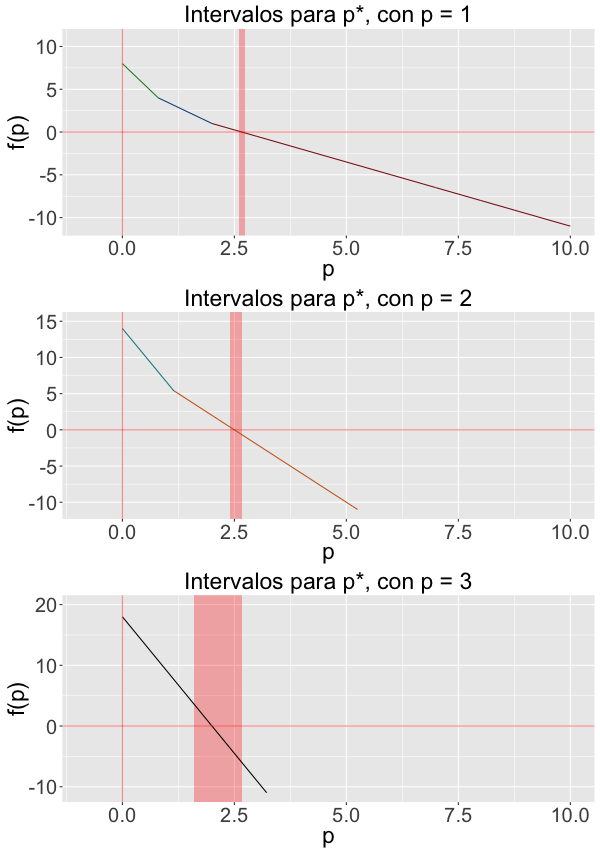
\includegraphics[width=.9\textwidth]{Figures/Chapter2_grid3eigen_interv}  
  \caption[Intervalos para $\rho^*$.] {La figura superior representa intervalos para $\rho^*$ cuando $f(\rho) = \lambda_{G(\rho)_1}$, la de enmedio cuando $f(\rho) = \lambda_{G(\rho)_1} + \lambda_{G(\rho)_2}$ y la de abajo cuando $f(\rho) = \lambda_{G(\rho)_1} + \lambda_{G(\rho)_2} + \lambda_{G(\rho)_3}$.}
\end{figure}

\end{example}

Otro intervalo que se ha desarrollado tiene que ver con directamente con los eigenvalores de $A$ y $B$ en lugar de los obtenidos por la matriz $A-\rho B$:

\pagebreak
\begin{proposition}
Sea $B$ positiva definida, entonces la raíz $\rho^*$ de $f(\rho)$ es tal que \cite{ngo2012trace}:

\begin{equation*}
\frac{\sum_{i = 1}^{p}\lambda_{A_i}}{\sum_{i = 1}^{p}\lambda_{B_i}} \leq \rho^* \leq \frac{\sum_{i = 1}^{p}\lambda_{(A)_i}}{\sum_{i = 1}^{p}\lambda_{(B)_{n-i+1}}}	
\end{equation*}

con $\lambda_{A_i}$ y $\lambda_{B_i}$ el i-ésimo eigenvalor más grande  de la matriz $A$ y $B$ respectivamente \cite{ngo2012trace}. 
\end{proposition}


\begin{proof}
Se tiene la propiedad que para una $p$ dada:


\begin{equation}\label{eq:2.44}
\max_{V^T V = I} Tr(V^T A V) =  Tr(V^{T*} A V^*) = \sum_{i=1}^p \lambda_{A_i }
\end{equation}
 
Con $\lambda_{A_i}$ los eigenvalores de A. Como esta $V^*$ maximiza la traza sobre $A$, entonces no necesariamente maximiza la de $B$. Al sustituirla en $Tr(V^{T} B V)$ se tiene que: 

\begin{equation}\label{eq:2.45}
Tr(V^{T*} B V^*) \leq \sum_{i=1}^p \lambda_{B_i }
\end{equation}

Con $\lambda_{B_i}$ los eigenvalores de B. Al hacer el cociente de (1.43) y (1.44) Se puede acotar inferiormente a $\rho^*$:


\begin{equation*}
  \frac{\sum_{i=1}^p \lambda_{A_i}} {\sum_{i=1}^p \lambda_{B_i}} \leq \frac{Tr(V^{T*} A V^*)}{Tr(V^{T*} B V^*)} \leq \max_{V^T V} \frac{Tr(V^{T} A V)}{Tr(V^{T} B V)} = \rho^*
\end{equation*}

Ahora falta acotarlo superiormente. Usando las siguientes propiedades que son derivadas de (1.27):

\begin{equation}\label{eq:2.46}
  Tr(V^T A V) \leq \sum_{i=1}^p \lambda_{A_i} 
\end{equation}

\begin{equation}\label{eq:2.47}
  Tr(V^T B V) \geq \sum_{i=1}^p \lambda_{B_{(n-i+1)}}
\end{equation}

La expresión (1.46) es la suma de los p eigenvalores más chicos de $B$. Dividiendo (1.45) entre (1.46) se tiene que para cualquier matriz ortogonal $V$:

\begin{equation}\label{eq:2.48}
   \frac{Tr(V^{T} A V)}{Tr(V^{T} B V)} \leq \frac{\sum_{i=1}^p \lambda_{A_i}}{\sum_{i=1}^p \lambda_{B_{(n-i+1)}}}
\end{equation}

En particular si se toma $V = V^{**}$ (La matriz con la que se alcanza $\rho^*)$:

\begin{equation}\label{eq:2.49}
  \rho^* = \frac{Tr(V^{T**} A V^{**})}{Tr(V^{T**} B V^{**})} \leq \frac{\sum_{i=1}^p \lambda_{A_i}}{\sum_{i=1}^p \lambda_{B_{(n-i+1)}}}
\end{equation}

\end{proof}
\begin{example}
Para ejemplificar esta cota se usará las matrices $A$ y $B$ de los dos ejemplos anteriores y se muestra en la figura 1.7.


\begin{equation*}
A = \left(\!
    \begin{array}{ccc}
      4 & 0 & 0 \\
      0 & 6 & 0 \\
      0 & 0 & 8 
    \end{array}
  \!\right), \quad
B = \left(\!
    \begin{array}{ccc}
      1.5 & 0 & 0 \\
      0 & 2.5 & 0 \\
      0 & 0 & 5 
    \end{array}
\!\right) 
\end{equation*}


(i) Para $p = 1$ la cota es la siguiente:
\begin{equation*}
\begin{aligned}
  \lambda_{A_1} = 8 \qquad
  \lambda_{B_1} = 5 \qquad
  \lambda_{B_3} = 1.5
\end{aligned}
\end{equation*}

\begin{equation*}
\begin{aligned}
\rho_1 = \frac{\sum_{i = 1}^{p}\lambda_{A_i}}{\sum_{i = 1}^{p}\lambda_{B_i}}  = \frac{8}{5} \qquad
\rho_2 = \frac{\sum_{i = 1}^{p}\lambda_{A_i}}{\sum_{i = 1}^{p}\lambda_{B_{n-i+1}}}  = \frac{8}{1.5}
\end{aligned}
\end{equation*}

(ii) Para $p = 2$ la cota es la siguiente:

\begin{equation*}
\begin{aligned}
\sum_{i = 1}^{2}\lambda_{A_1}  =& 14 \qquad
\sum_{i = 1}^{2}\lambda_{B_1}  =& 7.5 \qquad
\sum_{i = 1}^{2}\lambda_{B_{3-i+1}} =& 4
\end{aligned}
\end{equation*}

\begin{equation*}
\begin{aligned}
\rho_1 = \frac{\sum_{i = 1}^{p}\lambda_{A_i}}{\sum_{i = 1}^{p}\lambda_({B_i)}}
 = \frac{14}{7.5} \qquad
\rho_2 = \frac{\sum_{i = 1}^{p}\lambda_{A_i}}{\sum_{i = 1}^{p}\lambda_{B_{n-i+1}}}  = \frac{14}{4}
\end{aligned}
\end{equation*}



(iii) Para $p = 3$ la cota es la siguiente:
\begin{equation*}
  \begin{aligned}
  \sum_{i = 1}^{3}\lambda_{A_1}  = 18 \qquad
  \sum_{i = 1}^{3}\lambda_{B_1}  = 9 \qquad
  \sum_{i = 1}^{3}\lambda_{B_{n-i+1}}  = 9
  \end{aligned}
\end{equation*}

\begin{equation*}
  \begin{aligned}
\rho_1 = \frac{\sum_{i = 1}^{p}\lambda_{A_i}}{\sum_{i = 1}^{p}\lambda_{B_i}}  = \frac{18}{9} \qquad
\rho_2 = \frac{\sum_{i = 1}^{p}\lambda_{A_i}}{\sum_{i = 1}^{p}\lambda_{B_{n-i+1}}}  = \frac{18}{9}
  \end{aligned}
\end{equation*}

\end{example}

\begin{figure}[!ht] \label{Fig1.7}
  \centering
  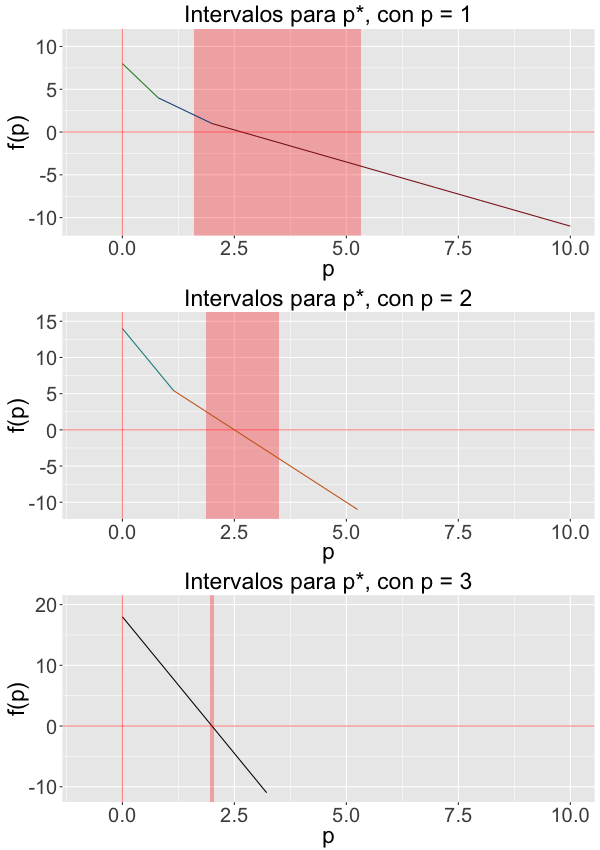
\includegraphics[width=.9 \textwidth]{Figures/Chapter2_grid3eigen_interv2}  
  \caption[Intervalos para $\rho^*$.] {La figura superior representa intervalos para $\rho^*$ cuando $f(\rho) = \lambda_{G(\rho)_1}$, la de enmedio cuando $f(\rho) = \lambda_{G(\rho)_1} + \lambda_{G(\rho)_2}$ y la de abajo cuando $f(\rho) = \lambda_{G(\rho)_1} + \lambda_{G(\rho)_2} + \lambda_{G(\rho)_3}$.}
\end{figure}




	%  \chapter{El Método Newton-Lanczos}
\label{ch:chapter3}
 
En el capítulo anterior se propuso una función no creciente $f(\rho)$ cuya raíz resulta ser la solución óptima para el problema del Discriminante Lineal de Fisher:

\begin{equation} \label{eq:3.1}
	f(\rho) = \max_{V^T V = I} Tr(V^T(S_E - \rho S_I)V)
\end{equation}

El algoritmo propuesto para encontrar la solución recibe el nombre de Newton-Lanczos\cite{ngo2012trace}. Para entenderlo a profundidad, se explicarán brevemente los métodos de Lanczos que tridiagonalizan una matriz simétrica, para después calcular eficientemente los primeros (últimos) eigenvalores. Después, será implementado junto al método iterativo de Newton, que calcula el nuevo valor de $\rho_{n}$ para cada paso. Para esto, se requiere el cómputo de la derivada de $f(\rho)$, por lo que se desarrollará su forma analítica. Finalizando, se proporcionarán las condiciones necesarias de optimalidad.

La primera división de los métodos para calcular eigenvectores y eigenvalores que propone J. Demmel \cite{demmel1997applied} depende si la matriz es simétrica o no lo es. Después hace una sub-clasificación dependiendo si el método es iterativo o directo. Para este texto solo se calcularán los eigenvalores de matrices simétricas, por lo que el procedimiento a seguir sera el siguiente:


\begin{itemize}
\item Tridiagonalizar la matriz simétrica por un método iterativo
\item Encontrar los eigenvalores por medio de la iteración tridiagonal QR (LAPACK DSTEVD)
\end{itemize}
\section{Métodos de Lanczos}
Antes de presentar los métodos de Lanczos, se dará una breve introducción acerca del costo computacional del algoritmo QR y la importancia de tridiagonalizar la matriz \cite{demmel1997applied}.  Sea $A \in {\rm I\!R}^{n \times n}$, entonces su descomposición $QR$ toma $O(n^3)$ flops. Suponiendo el mejor escenario en el que cada eigenvalor se encuentra con una iteración, tomaría $O(n^4)$ flops para calcular todos los eigenvalores de una matriz. Por otra parte, al tridiagonalizar la matriz $A$ se reduce el costo computacional de la descomposición $QR$ a $O(n^2)$ flops. De esta manera, tomaría $O(n^3)$ flops encontrar todos los eigenvalores. Una descripción más detallada del costo computacional de los algoritmos puede encontrarse en \cite{demmel1997applied}.

El primer paso, la tridiagonalización, ha sido muy estudiado y existen algoritmos especializados para distintos tipos de matrices simétricas. Si la matriz es de gran dimensión y rala, entonces se recomienda usar el método de Lanczos \cite{golub2012matrix}. En otro caso, existen las transformaciones Householder y las rotaciones de Givens \cite{golub2012matrix}. El método de Lanczos realiza tridiagonalizaciones parciales de la matriz original $A$, donde cada una es de tamaño $p \times p$ con $p\leq n$. Un aspecto interesante es que las matrices parciales van aproximando los eigenvectores extremos antes que la tridiagonalización esté completa. Por este motivo, el algoritmo es usado cuando se requieren solo algunos de los eigenvalores. Con respecto al costo computacional, es del orden $O(n^3)$, por lo que el algoritmo completo se mantiene en el mismo orden. 

Lanczos en aritmética exacta tiene muchas ventajas computacionales y converge rápidamente a los eigenvalores reales, pero con aritmética inexacta es difícil usarlo en la práctica \cite{golub2012matrix}. El problema que se presenta es que los eigenvectores van perdiendo la ortogonalidad entre ellos conforme la dimensionalidad y las iteraciones incrementan. Los textos \cite{demmel1997applied}\cite{golub2012matrix} incluyen algoritmos para solucionar este problema.

En la siguiente subsección se presentará el algoritmo original de Lanczos; se ejemplificará como los eigenvalores de la matriz tridiagonal convergen a los originales y se presenta el problema de \textit{ghost eigenvalues} \cite{demmel1997applied}, que son los eigenvalores que surgen al perder la ortogonalidad en aritmética inexacta.

\subsection{Algoritmo de Lanczos}

El algoritmo de Lanczos busca calcular los elementos de esta matriz tridiagonal directamente. Definiendo $Q^T A Q = T$, con $Q = [q_{(1)} \enskip|\enskip q_{(2)} \enskip|\enskip ... \enskip|\enskip q_{(n)}]$ ortogonal, y $T_n$ tridiagonal igual a:

\begin{equation}\label{eq:3.2}
T_n = \left(\!
    \begin{array}{cccccc}
      \alpha_1 & \beta_2 &  &  &  & 0\\
      \beta_2  & \alpha_2 & \beta_3 &  &  & \\
               & \beta_3 & \alpha_3 &  \ddots  & & \\
               &         & \ddots & \ddots & \beta_{n-1}& \\
               &  &  &  \beta_{n-1} & \alpha_{n-1} & \beta_n\\
       0       &  &  &  & \beta_n & \alpha_{n}\\
    \end{array}
  \!\right), \quad
\end{equation}

Como $q_{(1)}$ es una columna de Q, entonces $q_1^T = [q_{11},\enskip q_{21},\enskip ... ,\enskip q_{n1}]$. De esta manera, se tiene que $AQ = QT$. Descomponiendo la multiplicación $AQ =[Aq_{(1)} \enskip|\enskip Aq_{(2)} \enskip|\enskip ... \enskip|\enskip Aq_{(n)}]$ e igualándola a cada columna de $QT$, se tiene que $Aq_{(1)}$ \cite{golub2012matrix}:

\begin{equation*}
\begin{aligned}
Aq_{(1)} =\quad &  q_{(1)(1)} \alpha_{(1)}       &+\quad q_{(1)(2)} \beta_{(2)} \quad&+ \\
     & q_{(2)(1)}   \alpha_{(1)}       &+\quad q_{(2)(2)} \beta_{(2)} \quad&+ \\
     &          \qquad         \vdots&\vdots \qquad     & \\
     & q_{(n)(1)}   \alpha_{(1)}       &+\quad q_{(n)(2)} \beta_{(2)} \quad& \\
Aq_{(1)} =\quad & \alpha_{(1)} q_{(1)} &+\quad \beta_{(2)} q_{(2)}   \qquad& 
\end{aligned}
\end{equation*}

Ahora, para $i = 2, ..., n-1$
  
\begin{equation*}
\begin{aligned}
Aq_{(i)} =\quad &  q_{(i-1)(i-1)}\beta_{(i)}  &+ \enskip q_{(i-1)(i)}\alpha_{(i)} &+ \enskip q_{(i-1)(i+1)} \beta_{(i+1)} &+ \\
     & q_{(i)(i-1)}\beta_{(i)}       &+ \enskip q_{(i)(i)}\alpha_{(i)}\enskip   &+\enskip q_{(i)(i+1)} \beta_{(i+1)}   &+ \\
     & \vdots &          \qquad \qquad \quad \vdots & &\\
     & q_{(n)(i-1)}\beta_{(i)}      &+\enskip q_{(n)(i)}\alpha_{(i)} \enskip  &+\enskip q_{(n)(i+1)} \beta_{(i+1)}   & \\
Aq_{(i)} =\quad & \beta_{(i)} q_{(i-1)}      &+ \enskip\quad \alpha_{(i)} q_{(i)} \quad    &+\enskip \beta_{(i+1)} q_{(i+1)}      &
\end{aligned}
\end{equation*}

Por último, para $Aq_n$:

\begin{equation*}
\begin{aligned}
Aq_{(n)} =\quad &  q_{(1)(n)} \alpha_{(n)}       &+\quad q_{(1)(n-1)} \beta_{(n)} \quad&+ \\
     & q_{(2)(n)}   \alpha_{(n)}       &+\quad q_{(2)(n-1)} \beta_{(n)} \quad&+ \\
     &          \qquad         \vdots&\vdots \qquad     & \\
     & q_{(n)(n)}   \alpha_{(n)}       &+\quad q_{(n)(n-1)} \beta_{(n)} \quad& \\
Aq_{(n)} =\quad & \alpha_{(n)} q_{(n)} &+\quad \beta_{(n)} q_{(n-1)}   \qquad& 
\end{aligned}
\end{equation*}


Si se define $q_{(0)} = 0$, entonces se puede resumir el paso como:

\begin{equation}\label{eq:3.3}
  Aq_{(i)} = \beta_{(i)} q_{(i-1)} + \alpha_{(i)} q_{(i)}+ \beta_{(i+1)} q_{(i+1)}
\end{equation}

para $i = 1, .... n-1$. Multiplicando esta expresión por $q_{(i)}^T$, y usando el supuesto de ortogonalidad, entonces $q_{(i)}^T q_{(j)} = 0$ con $i \neq j$. De esta manera resulta la siguiente expresión:

\begin{equation}\label{eq:3.4}
\begin{aligned}
  q_{(i)}^TAq_{(i)} &=  q_{(i)}^T\alpha_{(i)} q_{(i)}  
                    &= \alpha_{(i)}
\end{aligned}
\end{equation}

Por otra parte, despejando $\beta_{(i+1)} q_{(i+1)}$ de \ref{eq:3.3}, se tiene que

\begin{equation}\label{eq:3.5}
\begin{aligned}
\beta_{(i+1)} q_{(i+1)}  =& Aq_{(i)} - \beta_{(i)} q_{(i-1)} - \alpha_{(i)} q_{(i)} \\ 
=& (A - \alpha_{(i)} I) q_{(i)} - \beta_{(i)} q_{(i-1)} = r_{(i)}
\end{aligned}
\end{equation}

Con la ecuación \ref{eq:3.5}, $q_{(i+1)} = \frac{r_{(i)}}{\beta_{(i+1)}}$. Calculando la norma de $r_{(i)}$, se tiene que 

\begin{equation}\label{eq:3.6}
\begin{aligned}
||r_{(i)}||_2 =& |\beta_{(i+1)}| ||q_{(i+1)}||_2 \\
              =& |\beta_{(i+1)}|
\end{aligned}
\end{equation}
 
Cuando $r_k =0$ entonces la iteración se detiene. \cite{golub2012matrix}

\pagebreak

\textbf{Implementación en aritmética exacta}\\

Sea $ A \in {\rm I\!R}^{n \times n}$ una matriz simétrica y $q_i \in {\rm I\!R}^{n}$. Entonces el algoritmo que se presenta a continuación produce una matriz $T_k \in {\rm I\!R}^{k \times k}$ tridiagonal tal que los eigenvalores de $T_k$ convergen a los de la matriz original $A$ \cite{golub2012matrix}. 

\begin{algorithm}[H] 
 $q_0$ $\leftarrow$ $0$\;
 $r_0$ $\leftarrow$ vector aleatorio\;
 $\beta_1$ $\leftarrow$ $||r_0||_2$\;
 $q_1 \leftarrow r_0 / \beta_1$\;
 $\alpha_1 \leftarrow q_1^T A q_1$\;
 $eps = 0.0000001$\;
 $k = 1$ \;
 \While{($\beta_k > eps$)}{
  $r_k \leftarrow A q_k - \alpha_k q_k - \beta_k q_{k-1}$\;
  $\beta_{k+1} \leftarrow ||r_{k-1}||_2$\;
  $q_{k+1} \leftarrow r_{k+1}/\beta{k+1}$\;
  $\alpha_{k+1} \leftarrow q_{k+1}^T A q_{k+1}$\;
  $k \leftarrow k+1$\;
 }
 \caption{Algoritmo de Lanczos}
\end{algorithm}

Para hacer frente a la pérdida de ortogonalidad entre los vectores, se han creado distintos métodos, los cuales se basan en la reortogonalización de la base de vectores. \cite{demmel1997applied} Esta puede realizarse en $O(n^2)$ operaciones, por lo que no afecta el orden de $O(n^3)$ flops.

\section{Derivada de $f(\rho)$}

La fórmula analítica de la derivada de $f(\rho)$ se puede obtener con cálculo multivariado. Para encontrarla, sea $V(\rho) \in {\rm I\!R}^{n \times p}$ una función diferenciable con respecto a $\rho$. Esta cumple la característica de ser una matriz ortogonal con columnas:

\begin{equation*}
	V(\rho) = (v_1(\rho) \enskip|\enskip v_2(\rho) \enskip|\enskip ... \enskip|\enskip v_p(\rho))
\end{equation*}

Antes de calcular la derivada de $f(\rho)$, es conveniente examinar la derivada de $V(\rho)^T V(\rho)$ con respecto a $\rho$. Sea $V(\rho)$ una matriz ortogonal; es decir, que cumpla $V^T(\rho) V(\rho) = I$, entonces \cite{ngo2012trace}:

\begin{equation*}
\frac{d}{d\rho} V(\rho)^T V(\rho) = \left(\frac{d}{d\rho}V(\rho)^T\right) V(\rho)  + V(\rho)^T 	\left( \frac{d}{d\rho} V(\rho) \right)
\end{equation*}

\vspace{5mm}

La derivada de $V(\rho)$ no se conoce explícitamente, pero se puede derivar componente a componente. De esta manera:


\begin{equation*}
\begin{aligned}
V(\rho)^T V(\rho)  &= \left(\!
    \begin{array}{cccc}
      v_{11}(\rho) & v_{21}(\rho) & \hdots & v_{n1}(\rho) \\
      v_{12}(\rho) & v_{22}(\rho) & \hdots & v_{n2}(\rho) \\
      \vdots & \vdots & \vdots & \vdots \\
      v_{1p}(\rho) & v_{2p}(\rho) & \hdots & v_{np}(\rho) 
    \end{array}
  \!\right)
    \left(\!
    \begin{array}{cccc}
      v_{11}(\rho) & v_{12}(\rho) & \hdots & v_{1p}(\rho) \\
      v_{21}(\rho) & v_{22}(\rho) & \hdots & v_{2p}(\rho) \\
      \vdots & \vdots & \vdots & \vdots \\
      v_{n1}(\rho) & v_{n2}(\rho) & \hdots & v_{np}(\rho) 
    \end{array} 
    \!\right) \\
    \vspace{5mm}
 &= \left(\!
    \begin{array}{c}
      v_{1}(\rho)^T \\
      v_{2}(\rho)^T \\
      \vdots \\
      v_{p}(\rho)^T  
    \end{array}
  \!\right)
  \left(\!
    \begin{array}{cccc}
      v_{1}(\rho) & v_{2}(\rho) & \hdots & v_{p}(\rho) 
    \end{array} 
	\!\right) 
\end{aligned}
\end{equation*}

Entonces la entrada $(i,j)$ de $V(\rho)^T V(\rho)$ es:

\begin{equation*}
	[V(\rho)^T V(\rho)]_{ij} = v_i(\rho)^T v_j(\rho)
\end{equation*}

Calculando la derivada:

\begin{equation*}
\frac{d}{d\rho}[V(\rho)^T V(\rho)]_{ij} =  \left( \frac{d}{d\rho}v_i(\rho)^T \right)  v_j(\rho) + v_i(\rho)^T \left( \frac{d}{d\rho} v_j(\rho)\right) 
\end{equation*}

En específico para el caso $i = j$:
\vspace{5mm}
\begin{equation}\label{eq:3.7}
\frac{d}{d\rho}[V(\rho)^T V(\rho)]_{ii} =  2 \left( \frac{d}{d\rho}v_i(\rho)^T \right)  v_i(\rho)
\end{equation}

\bigskip

\begin{lemma}\label{lemma:3.1}
Sea $V(\rho) \in {\rm I\!R}^{n \times p}$ una matriz ortogonal y $\rho$ su parámetro. Entonces \cite{ngo2012trace}:
\begin{equation*}
\begin{aligned}
(i)&  \quad \frac{d}{d\rho} V(\rho)^TV(\rho) = \left(\frac{d}{d\rho}V(\rho)^T\right) V(\rho)  + V(\rho)^T  \left( \frac{d}{d\rho} V(\rho) \right) = 0 \\
(ii)& \quad Diag \left(\left(\frac{d}{d\rho}V^T \right)V(\rho) \right) = 0 
\end{aligned}
\end{equation*}
\end{lemma}

\begin{proof}
\bigskip
(i) Para demostrar la primer propiedad se hace uso de que $V(\rho)^T V(\rho) = I_p$, entonces:
\begin{equation*}
\frac{d}{d\rho} [V(\rho)^T V(\rho)] = 0  
\end{equation*}

(ii) Se parte de la ecuación (\ref{eq:3.7}), y se usa el punto (i):
\begin{equation*}
  \frac{d}{d\rho} [V(\rho)^T V(\rho)]_{ii} =    2 \left( \frac{d}{d\rho}v_i(\rho)^T \right)  v_i(\rho) = 0
\end{equation*}

Como cada elemento $i$ es cero, entonces en particular $Diag\left( \left(\frac{d}{d\rho}V(\rho)^T \right) V(\rho) \right)=0 $.
\end{proof}

Del lema \ref{lemma:3.1} se tiene que $\left(\frac{d}{d\rho}V(\rho)^T \right) V(\rho)$ tiene diagonal igual a 0. Ahora, para derivar $f(\rho)$, primero se deriva la expresión $\frac{d}{d\rho}\left[V^T (A-\rho B)V \right]$:

\begin{equation}\label{eq:3.8}
\begin{aligned}
	\frac{d}{d\rho}\left[V^T (A-\rho B)V \right] & = \frac{d}{d\rho} \left[V^T A V \right]- \frac{d}{d\rho}\left[V^T \rho B V\right] \\
	& = \frac{dV^T}{d\rho}  AV +  V^T A \frac{dV}{d\rho} - \frac{dV^T}{d\rho} \rho BV - V^T \left[BV + \rho B \left(\frac{dV}{d\rho} \right) \right] \\
	& = \frac{dV^T}{d\rho} \left[A -\rho B \right] V + V^T \left[A- \rho B \right]\frac{dV}{d\rho} - V^TBV \\
\end{aligned} 
\end{equation}


Sea $V$ la matriz que diagonaliza $(A-\rho B)$, de manera que $V^T (A-\rho B) V = D$. Entonces \ref{eq:3.8}:
\begin{equation}\label{eq:3.9}
\begin{aligned}
\frac{d}{d\rho}\left[V^T (A-\rho B)V \right] & = \frac{dV^T}{d\rho} VD  + DV^T\frac{dV}{d\rho} - V^TBV 
\end{aligned}
\end{equation}

Al calcular la traza de (\ref{eq:3.9}) y usando del lema \ref{lemma:3.1}, se tiene que:
\begin{equation}\label{eq:3.10}
\begin{aligned}
Tr\left[\frac{d}{d\rho} \left[V^T (A-\rho B)V \right]\right] & = Tr\left[ \frac{dV^T}{d\rho} VD + DV^T \frac{dV}{d\rho} - V^T B V  \right] \\
											     & = 2 Tr \left[ D V^T \frac{dV}{d\rho} \right] - Tr \left[ V^T B V \right] \\
											     & = -Tr\left[V^T B V \right] 
\end{aligned}	
\end{equation}

\section{Método Newton-Lanczos}

El método de Newton establece que la iteración está dada por:

\begin{equation*}
x_{(n+1)} = x_{(n)} - \frac{f(x_n)}{f'(x_n)}
\end{equation*}

con $f'(x_n)$ la derivada de $f(x_n)$.

Con esta fórmula y con (\ref{eq:3.10}), se puede calcular explícitamente $\rho_{n+1}$ para la iteración de Lanczos \cite{ngo2012trace}:

\begin{equation}\label{eq:3.11}
\begin{aligned}
\rho_{n+1} =& \rho_{n} - \frac{Tr\left[V^T (A-\rho_n B)V \right]}{-Tr\left[V^T B V \right]} \\ \\
           =& \frac{\rho_{n} Tr\left[V^T B V \right] +  Tr\left[V^T (A-\rho_n B)V \right]}{Tr\left[V^T B V \right]}\\ \\
           =& \frac{\rho_{n} Tr\left[V^T B V \right] +  Tr\left[V^T A V \right] - \rho_nTr\left[V^T BV \right]}{Tr\left[V^T B V \right]} \\ \\
           =&\frac{Tr\left[V^T A V \right]}{Tr\left[V^T B V \right]}
\end{aligned} 
\end{equation}

Una vez calculado el paso de la iteración, se enuncia el método de Newton-Lanczos para maximizar el cociente de trazas. El método recibe como entrada la matriz $A$, $B$ y la dimensión a la cual se desea proyectar $p$ \cite{ngo2012trace}: 

\begin{algorithm}[H]
i = 1\;
$\rho_1$ un número aleatorio\;
$\rho_0$\;
$f(\rho_1) = \sum\limits_{j = 1}^{p} \lambda_{(A-\rho_1 B)_j}$\;
V = primeros $p$ eigenvectores de $A-\rho_1 B$\;
$tol = 1e-10$\;

\While{($i<50$ \quad , \quad $abs(\rho_i-\rho_{i-1}$)$>tol$)}{
$i = i+1$\;
V = primeros $p$ eigenvectores de $(A-\rho_i B)$ \;
$\rho_i = Tr(V^T A V)/Tr(V^T BV)$\;
$f(\rho_i) = \sum\limits_{j = 1}^{p} \lambda_{(A-\rho_i B)_j}$\;
}
 \caption{Algoritmo de Newton-Lanczos}
\end{algorithm}


\subsection{Condiciones necesarias de optimalidad}
Considerando el problema de maximizar las trazas:

\begin{equation}\label{eq:3.12}
  \max_{\substack{V \in {\rm I\!R}^{n \times p} \\ V^TV = I}} \frac{Tr(V^T S_E V)}{Tr(V^T S_I V)} 
\end{equation}

La función lagrangiana asociada a este problema es la siguiente \cite{ngo2012trace}:

\begin{equation*}
L(V, \Gamma) =  \frac{Tr(V^T S_E V)}{Tr(V^T S_I V)} - Tr[\Gamma(V^TV-I)]
\end{equation*}

Con $\Gamma \in {\rm I\!R}^{p \times p}$ , la matriz de multiplicadores de Lagrange de la forma:

\begin{equation*}
\Gamma = \left(\!
    \begin{array}{ccccc}
    \gamma_{(1)(1)} & \gamma_{(1)(2)} & \hdots & \gamma_{(1)(p-1)} & \gamma_{(1)(p)} \\
    \gamma_{(2)(1)} & \gamma_{(2)(2)} & \hdots & \gamma_{(2)(p-1)} & \gamma_{(2)(p)} \\
    \vdots & \vdots & \vdots & \vdots & \vdots \\
    \gamma_{(p-1)(1)} & \gamma_{(p-1)(2)} & \hdots & \gamma_{(p-1)(p-1)} & \gamma_{(p-1)(p)} \\
    \gamma_{(p)(1)} & \gamma_{(p)(2)} & \hdots & \gamma_{(p)(p-1)} & \gamma_{(p)(p)} \\
\end{array}
  \!\right), \quad
\end{equation*}


Ya que al multiplicar esta matriz por $[V^T V- I]$ (con $V = (v_1 \enskip |\enskip v_2 \enskip |\enskip ... \enskip |\enskip v_{p-1} \enskip |\enskip v_p)$) se tiene que: 

\begin{equation*}
V^T V - I = \left(\!
    \begin{array}{ccccc}
    v_1^T v_1 -1& v_1^T v_2 & \hdots & v_1^T v_{p-1} & v_1^T v_p \\
    v_2^T v_1 & v_2^T v_2 -1& \hdots & v_2^T v_{p-1} & v_2^T v_p \\
    \vdots & \vdots & \vdots & \vdots & \vdots \\
    v_{p-1}^T v_1 & v_{p-1}^T v_2 & \hdots & v_{p-1}^T v_{p-1} -1& v_{p-1}^Tv_p \\
    v_p^T v_1 & v_p^T v_2 & \hdots & v_p^Tv_{p-1} & v_{p}^Tv_{p} -1 \\
\end{array}
  \!\right), \quad
\end{equation*}

entonces, la diagonal de ($\Gamma (V^T V - I)$) contiene $p$ elementos que son los siguientes: 

\begin{equation*}
\left(\!
    \begin{array}{c}
    \begin{aligned}
    & \gamma_{(1)(1)}(v_1^T v_1 -1) &+& \gamma_{(1)(2)} (v_2^T v_1) &+& \hdots &+& \gamma_{(1)(p)}(v_p^T v_1) &\\
    & \gamma_{(2)(1)}(v_1^T v_2) &+& \gamma_{(2)(2)}(v_2^T v_2 -1)  &+& \hdots &+& \gamma_{(2)(p)}(v_p^T v_2) &\\
    & \vdots && \vdots && \vdots && \vdots &\\
    &\gamma_{(p-1)(1)}(v_1^T v_{p-1}) &+& \gamma_{(p-1)(2)} (v_2^T v_{p-1}) &+& \hdots &+& \gamma_{(p-1)(p)}(v_p^T v_{p-1})&\\
    &\gamma_{(p)(1)}(v_1^T v_{p}) &+& \gamma_{(p)(2)}(v_2^T v_p)  &+& \hdots &+& \gamma_{(p)(p)}(v_p^T v_{p}-1) &\\
\end{aligned}
\end{array}
  \!\right), \quad
\end{equation*}

Para calcular la traza se suman estos elementos de la diagonal. De esta forma, se tienen p restricciones de la forma $v_i^T v_i = 1 \quad i = 1,...,p$ y $p(p-1)$ restricciones de la 
forma $v_i^T v_j = 0 \quad i \neq j, \quad i,j = 1, ..., p$, cada una con su multiplicador lagrangiano.

Como la ecuación a maximizar tiene un maximizador global $V^*$, entonces existe un multiplicador matricial lagrangiano tal que en el óptimo:

\begin{equation}\label{eq:3.13}
\frac{\partial \mathcal{L}(V^*, \Gamma^*)}{\partial V} =  0 \qquad con \qquad V^{T*}V^* = I
\end{equation}

Para encontrar $(V^*, \Gamma^*)$ de (\ref{eq:3.13}), primero se debe conocer la derivada de $\frac{\partial Tr(V^T M V)}{\partial V}$, con M cualquier matriz:

\begin{equation}\label{eq:3.14}
\frac{\partial Tr(V^T M V)}{\partial V} = (M^* +M)V  
\end{equation}

\pagebreak
Derivando el lagrangiano (\ref{eq:3.13}) y utilizando (\ref{eq:3.14}) se tiene que:

\begin{equation*}
\begin{aligned}
\frac{\partial \mathcal{L}(V, \Gamma)}{\partial V} =&\quad  \left[\frac{\partial Tr(V^T A V) }{\partial V}\right]\left[Tr(V^T B V)^{-1}\right] \quad +& \\
&\quad \left[Tr(V^T A V)\right]\left[\frac{\partial (Tr(V^T B V))^{-1} }{\partial V}\right] \quad -& \\
&\quad \left[\frac{\partial Tr[\Gamma(V^TV-I)] }{\partial V}\right] \quad &
\end{aligned}
\end{equation*}
\vspace{5mm}

\begin{equation*}
\begin{aligned}
\frac{\partial \mathcal{L}(V, \Gamma)}{\partial V} =&\quad  \left[2AV\right]\left[Tr(V^T B V)^{-1}\right] \quad +& \\
&\quad \left[Tr(V^T A V)\right]\left[\frac{2BV}{Tr(V^T B V)^2}\right] \quad -& \\
&\quad \left[V (\Gamma^* + \Gamma) \right] \quad &
\end{aligned}
\end{equation*}
\vspace{5mm}

\begin{equation}\label{eq:3.15}
\begin{aligned}
\frac{\partial \mathcal{L}(V, \Gamma)}{\partial V} =&\quad  \left[\frac{2AV Tr(V^T B V)- 2BV Tr(V^T A V)}{(Tr(V^T B V))^2}\right] \quad +& \\
&\quad \left[V (\Gamma^* + \Gamma) \right] \quad &
\end{aligned}
\end{equation}

Igualando (\ref{eq:3.15}) a cero y acomodando la expresión, resulta:
\begin{equation*}
\left[A-\frac{Tr(V^{T*} A V^*)}{Tr(V^{T*} B V^*)}B\right] V^*  = \left[\frac{Tr(V^{T*} B V^*)}{2}V^* (\Gamma^{T*} + \Gamma^{*})\right]
\end{equation*}

\begin{equation}\label{eq:3.16}
\left[ A-\rho^* B\right]V^*   = \left[ \frac{Tr(V^{T*} B V^*)}{2}V^* (\Gamma^{T*} + \Gamma^{*}) \right]
\end{equation}

Con $\rho^* = \frac{Tr(V^{T*} A V^*)}{Tr(V^{T*} B V^*)}$. Sea $Q$ la matriz ortogonal que diagonaliza $\Gamma^{T*} + \Gamma^{*}$, entonces se puede escribir la expresión $(\Gamma^{T*} + \Gamma^*)$ como:
\begin{equation*}
 \left(\Gamma^{T*} + \Gamma^{*}\right) = Q \Sigma^* Q^T \qquad con \qquad Q^TQ = I
\end{equation*}

Con $\Sigma^*$ una matriz diagonal. Multiplicando (\ref{eq:3.16}) por $V^{T*}$ y calculando la traza de ambos lados de la ecuación y se tiene que:

\begin{equation*}
\begin{aligned}
Tr\left[ V^{T*}(A-\rho^* B)V^*\right]  =& \left[ \frac{Tr(V^{T*} B V^*)}{2}\right] Tr(\Gamma^{T*} + \Gamma^{*}) \\ \\
Tr(\Gamma^{T*} + \Gamma^{*}) =& 2 \frac{Tr(V^{T*}(A-\rho^*B)V^*)}{Tr(V^{T*}BV^*)} = 0 
\end{aligned}
\end{equation*}
\vspace{5mm}
\begin{equation}\label{eq:3.17}
Tr(Q \Sigma^* Q^T) = 2 \frac{Tr(V^{T*}(A-\rho^*B)V^*)}{Tr(V^{T*}BV^*)} = 0
\end{equation}


Como $Tr(V^{T*}(A-\rho^*B)V^*) = 0$ entonces $Tr(Q \Sigma^* Q^T) =0$, por lo que $Tr(\Sigma^*) = 0$. Definiendo $U^* = V^*Q$, con $U^*U = I$, la expresión (\ref{eq:3.16}) se puede escribir como:

\begin{equation*}
\begin{aligned}
\left[ A-\rho^* B\right]V^*   &= \left[ \frac{Tr(V^{T*} B V^*)}{2}V^* (Q \Sigma^* Q^T) \right] \\\\
                              &= \left[ \frac{Tr(V^{T*} B V^*)}{2}U^*Q^{T*} (Q \Sigma^* Q^T) Q \right] \\\\
                              &= \left[ \frac{Tr(V^{T*} B V^*)}{2}U^* \Sigma^* \right] \\
\end{aligned}
\end{equation*}  

Definiendo $\Lambda_* = \frac{Tr(V^{T*} B V^*)}{2}\Sigma^*$, entonces:
\begin{equation}\label{eq:3.18}
\begin{aligned}
\left[ A-\rho^* B\right]U^*   &= U^* \Lambda_* \\
 U^{T*} \left(A-\rho^* B\right)U^*   &=  \Lambda_* \\
 Tr(U^{T*} \left(A-\rho^* B\right)U^*)   &=  Tr(\Lambda_*) = 0
\end{aligned}
\end{equation}  

De esta manera se tiene que la ecuación (\ref{eq:3.18}) es la condición necesaria para que $U^*, \rho^*$ sean las óptimas










	%  \chapter{Experimentos numéricos}
\label{ch:chapter4}

Para medir el desempeño del algoritmo Newton-Lanczos se compara con otros dos métodos, el Análisis Discriminante Lineal (ADL) y la Regresión Logística Multinomial (RLM). Los criterios para elegir el mejor serán la tasa de reconocimiento y el tiempo de cómputo sobre los conjuntos de datos JAFFE y MNIST. Como el algoritmo de Newton-Lanczos ocupa los eigenvectores de una matriz, en la primer parte de este capítulo se medirá el tiempo de Lanczos y el costo de la rutina $SVD$ de R para una matriz en particular \footnote{La rutina $svd$ de $R$ ocupa la función $gesdd$ de la librería $LAPACK$. Para más información puede consultarse la página $http://www.netlib.org/lapack/$.}. En la segunda parte del capítulo, se explicará el preprocesamiento de las bases de datos y como se crearon los conjuntos de entrenamiento y prueba. En la tercer y cuarta parte, se realizan los experimentos con la bases de MNIST y JAFFE respectivamente. 

Para todos los experimentos de este capítulo, se utilizó el lenguaje de \textsf{R} en su versión 3.2.2 \textit{Fire Safety}. Los cálculos fueron realizados en una iMac 3.2 Ghz Intel Core i3 con 12 GB de RAM.

\section{Desempeño del método de Lanczos}

Antes de analizar el tiempo de cómputo de Newton-Lanczos, se evaluará el desempeño del algoritmo de Lanczos comparándolo con la factorización $svd$. Esto experimento es para saber en que casos es conveniente utilizar Lanczos y en cuales conviene calcular todos eigenpares. Para la prueba se usó $A - \rho B$ con $A$ y $B$ las matrices de dispersión intra clase y entre clase de la base de datos MNIST y con $\rho = 3$. La figura \ref{fig5.1} resume el desempeño de ambos métodos.

\begin{figure}[!ht] \label{fig5.1}
  \centering
  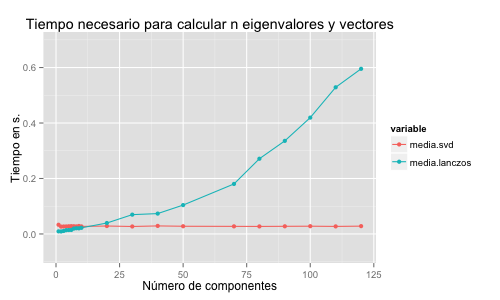
\includegraphics[width=1\textwidth]{Figures/Chapter4_eigen_lanczos.png} 
  \caption[Desempeño de Lanczos.] {Desempeño de Lanczos. En el eje $x$ se representa k, el número de eigenpares a calcular de la matriz $A- \rho B$. La matriz original es de 193 x 193. El tiempo reportado para cada $k$, es el promedio de $30$ repeticiones para cada método.}
\end{figure}

Se observa que, para $k$ menor a 10, el algoritmo de Lanczos es más rápido que la factorización $SVD$ de la matriz completa. Para valores más grandes, conviene factorizar toda la matriz. Esto puede deberse a que en aritmética inexacta Lanczos presenta el problema de \textit{Ghost eigenvalues} (eigenvalores que se repiten, pero que son espurios) \cite{golub2012matrix}. Estos se originan porque la ortogonalidad entre los eigenvectores se pierde conforme la dimensionalidad aumenta. Para solucionar este problema, se tuvo que realizar una reortogonalización completa en cada iteración, lo que pudo aumentar el tiempo de cómputo. 

\section{Modelos comparados y preprocesamiento de las bases}

En este capítulo, el método de Newton-Lanczos se comparó otros dos métodos de clasificación: la RLM y con el ADL. Para el primero, se usó la función \textit{multinom} del paquete \textit{nnet}, mientras que para el segundo se utilizó una modificación de la función \textit{lda} \footnote{La modificación está presentada en los códigos del apéndice B} del paquete \textit{MASS}. Ambas funciones fueron desarrolladas por Brian Ripley, profesor de estadística aplicada de la Universidad de Oxford. 

Como primer paso, se definieron los tamaños del conjunto de entrenamiento y prueba. Para el entrenamiento de MNIST se ocuparon 4000 datos (400 por clase); es decir, el 6\% del total. En el caso de JAFFE se utilizaron 50 datos (5 por clase); es decir, el 23\% del total. En ambos, el resto de los datos se ocupó en el conjunto de prueba. 

Para el preprocesamiento de las bases, cada imagen se convirtió en un vector con tamaño asociado al número de píxeles. Esto genera un problema de dimensionalidad, por lo que se realizó un paso de reducción dimensional. Se tomaron las primeras componentes principales (PCA) del conjunto de entrenamiento de manera que se explicara el 95\% de la varianza total, después se proyectó el conjunto de prueba. (De esta manera, los individuos en lugar de pertenecer a un espacio de ${\rm I\!R}^{m \times n}$, pertenecen a uno menor). Para MNIST se tomaron 193 de las 784 componentes; en cambio, para JAFFE solo 50 de las 65536. 

Una vez hecho el preprocesamiento, se realizaron 2 experimentos para cada base de datos. En el primero se utilizó el método de Newton-Lanczos con $V \in {\rm I\!R}^{m \times 20}$. Después de esto se proyectaron a los individuos originales a un espacio 20-dimensional. Los objetivos fueron los siguientes: 

\begin{itemize}
\item Analizar como cambia el valor de $f(\rho)$ con el método de Newton-Lanczos
\item Ver como se ven proyectados los datos en dimensiones menores
\end{itemize}

En el segundo experimento se entrenaron los 3 métodos con distintas $p$. Después se midió la tasa de reconocimiento alcanzada (usando el conjunto de prueba) y su tiempo de ejecución. 

\section{Base de datos MNIST}

Las siglas MNIST provienen de (\textit{Mixed National Institute of Standards and Technology}), la cual contiene datos de 70,000 dígitos escritos a mano que se usan comúnmente para probar códigos de clasificación de imágenes. De esta manera, en el experimento se tendrán 10 clases: los dígitos del 0-10. La base de datos surge de la colaboración de Yann LeCun del Instituto Courant (NYU), de Corinna Cortes de Google Labs (NY) y de Christopher J.C. Burges de Microsoft Research en Redmond. Puede descargarse de la página Web \textit{yann.lecun.com/exdb/mnist}, cuyo link sigue vigente al 13 de marzo del 2016.

Las imágenes están en un formato especial llamado IDX. Para poderlas convertir en un archivo leíble para R, se utilizó la función \textit{readMNIST} del paquete \textit{darch}. Esta paquetería convierte los archivos a objetos \textit{.RData}. La figura 3.2 contiene una extracto de tamaño 225 de todo el conjunto.

\begin{figure}[!ht]\label{fig5.2}
  \centering
	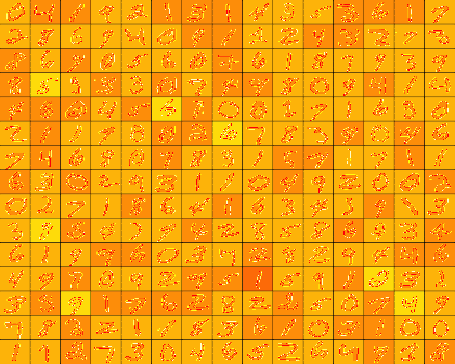
\includegraphics[width=1\textwidth]{Figures/Chapter4_numeros.png}	
  \caption{Ejemplo de números de la base de datos (MNIST).}
\end{figure}

\subsection{Proyección sobre un espacio de dimensión 20}

\underline{\textbf{1) Cotas para $\rho^*$}}

En el capítulo 2 se presentaron cotas para $\rho^*$ y en esta sección se ejemplificará la segunda de ellas para esta base de datos. Se calcularon los eigenvalores de la matriz intraclase (B) y de la matriz entre clases (A). Los 20 eigenvalores más grandes y más pequeños de la primera son \footnote{los eigenvalores menores a $1e^{-10}$ se consideraron numéricamente como 0}:

\begin{center}
\begin{tabular}{ | c | c|  c |c | c|  c |c | c|  c |c | c | c|  c |c | c|  c |c | c|  c |c |} 
\hline
12694 & 10367 & 7822 & 6793 & 6013 & 5887 & 5269 & 4704 & 4474 & 3969 \\
3833 & 3428 & 3124 & 3015 & 2978 & 2627 & 2535 & 2353 & 2232 & 2150 \\
\hline
\hline
\end{tabular}
\end{center}

\begin{center}
\begin{tabular}{ | c | c|  c |c | c|  c |c | c|  c |c | c | c|  c |c | c|  c |c | c|  c |c |} 
\hline
73 & 72 & 72 & 71 & 71 & 70 & 70 & 69 & 68 & 68 \\
67 & 67 & 66 & 66 & 65 & 64 & 64 & 63 & 63 & 62 \\
\hline
\hline
\end{tabular}
\end{center}

Mientras que los 9 eigenvalores más grandes de la matriz entre clases (A) son (los demás son 0):

\begin{center}
\begin{tabular}{ | c | c|  c |c | c|  c |c | c|  c |} 
\hline
12865 & 9821 & 7408 & 4736 & 3558 & 2312 & 1879 & 885 & 631 \\
\hline
\hline
\end{tabular}
\end{center}

Sustituyendo estos valores en la fórmula de las cotas de la raíz, se tiene que:

\begin{equation*}
\frac{\sum_{i = 1}^{p}\lambda_{A_i}}{\sum_{i = 1}^{p}\lambda_{B_i}} \leq \rho^* \leq \frac{\sum_{i = 1}^{p}\lambda_{(A)_i}}{\sum_{i = 1}^{p}\lambda_{(B)_{n-i+1}}}	
\end{equation*}

\begin{equation*}
\frac{44099.28}{96277.31} \leq \rho^* \leq \frac{44099.28}{1364.54}
\end{equation*}

\begin{equation*}
0.4580443 \leq \rho^* \leq 32.31806
\end{equation*}

A continuación se presentan como se ven $(\rho^*, f(\rho))$ con cada iteración para el método de Newton-Lanczos. 

\pagebreak

\underline{\textbf{2) Valores de $(\rho^*, f(\rho))$}}

Para el punto inicial de este experimento se utilizará el punto medio del intervalo. Los criterios de paro se fijaron con una tolerancia de $1e^{-10}$ y que las iteraciones sean menor a 50. Con este ejemplo, se obtienen los siguientes resultados para $\rho$ y $f(\rho)$:

\begin{center}
\begin{tabular}{ | c | c|  c |} 
\hline
$iter$ & $\rho$ & $f(\rho)$  \\ 
\hline
\hline
1 & $16.38805180$ & $-22,326.51$  \\ 
\hline
2 & $0.03121373$ & $42,841.16$  \\ 
\hline
3 & $1.11003833$ & $15,197.50$  \\ 
\hline
4 & $2.05957127$ & $3,926.463$  \\ 
\hline
5 & $2.50843464$ & $444.8128$  \\ 
\hline
6 & $2.57388828$ & $9.007894$  \\ 
\hline
7 & $2.57526971$ & $.004008613$  \\ 
\hline
8 & $2.57527033$ & $7.891856e^{-10}$  \\ 
\hline
9 & $2.57527033$ & $5.371703e^{-12}$  \\ 
\hline
\hline

\end{tabular}
\end{center}

\begin{figure}[!ht] \label{fig5.3}
  \centering
	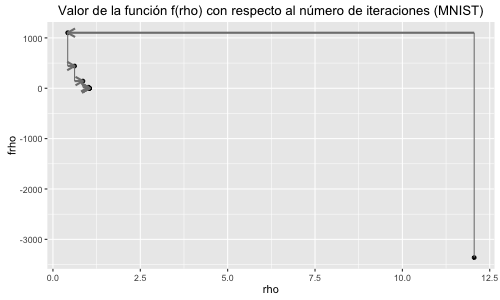
\includegraphics[width=.75\textwidth]{Figures/Chapter4_Iteraciones.png}	
  \caption[Valores de $\rho$ y $f(\rho)$ para distintas iteraciones (MNIST).] 
  {Valores de $\rho$ y $f(\rho)$ para distintas iteraciones (MNIST). El punto rojo es el punto inicial. Datos del conjunto de entrenamiento.}
\end{figure}

En la figura 3.3 se muestran $(\rho, f(\rho))$ para cada una de las 9 iteraciones. El punto inicial es el rojo, en este caso $\rho = 16.39$, mientras que $f(\rho)$ toma el valor de $-22,326$. Tras la primer iteración, $\rho$ toma el valor de $0.03$, y $f(\rho)$ es igual $42,841$. Conforme hay más iteraciones, $\rho$ y $f(\rho)$ convergen a los óptimos.

\underline{\textbf{3) Datos proyectados en 4 dimensiones}}

Se maximizó la traza del cociente para un espacio de 20 dimensiones. En la figura 3.4 se muestra como se agrupan los individuos del conjunto de entrenamiento conforme las iteraciones avanzan. 
  
\begin{figure}[!ht] \label{fig5.4}
  \centering
	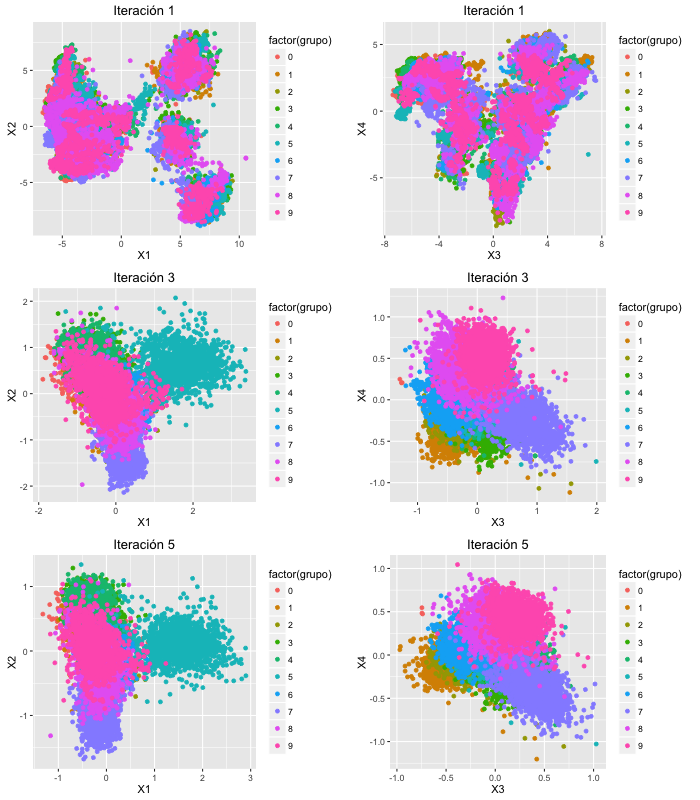
\includegraphics[width=1\textwidth]{Figures/Chapter4_ejemplo20componentes.png}	
  \caption[Ejemplo de proyección en 20 dimensiones (MNIST).]
  {Ejemplo de proyección en 20 dimensiones (MNIST). Las dos imágenes superiores son los datos de entrenamiento proyectadas sobre las 4 primeras componentes tras la primer iteración. Las dos intermedias son en la iteración 3 y las últimas 2 son la última iteración. Datos del conjunto de entrenamiento.}
\end{figure}

\subsection{Comparación con otros métodos}

Para la comparación de Newton-Lanczos con la RLM y el ADL se tomaron las siguientes consideraciones:

\begin{itemize}
\item Las dimensiones a considerar (k) son: 2, 5, 10, 15, 20, 40, 60, 80, 100, 120, 140, 160, 180 y 193
\item El número de variables que entran en cada modelo es el mismo (dada la dimensión k)
\item Los modelos se ajustan con el conjunto de entrenamiento y se calcula el error con el de prueba
\item Para Newton-Lanczos y ADL se proyectarán a un espacio k-dimensional y se usará 3-vecinos más cercanos para clasificarlos
\item Para el caso de regresión logística multinomial se elegirá la clase que tenga una mayor probabilidad posterior de selección
\end{itemize}

\underline{\textbf{1) Tasa de reconocimiento}}

La tasa de reconocimiento se mide como el número de individuos clasificados correctamente entre el número total del conjunto de test. Como el objetivo de esta sección es observar como se modifica la tasa con respecto aumenta k, se fijó el número de vecinos más cercanos a 3 para el caso de ADL y de Newton-Lanczos y también el tamaño del conjunto de entrenamiento. En la figura 3.5 se muestra que el modelo RLM y el ADL se comportan mejor para dimensiones pequeñas. Para casos de k mayor a 120, el método de Newton-Lanczos alcanza una mejor tasa de reconocimiento.

Es interesante observar que si se busca la mejor proyección con para k = 1 y k = 2, Newton-Lanczos resulta ser muy buen método. En la 3.4 se observó como los individuos se agrupan con este método. 


\begin{figure}[!ht] \label{fig5.5}
  \centering
	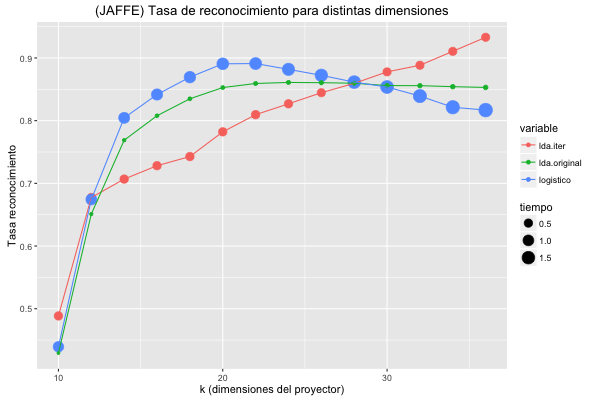
\includegraphics[width=1\textwidth]{Figures/Chapter4_Comparacion.png}	
  \caption[Tasa de reconocimiento base (MNIST).]
  {Tasa de reconocimiento base (MNIST). En azul se representa el RLM, en verde el ADL y en rojo el método de Newton-Lanczos. En el eje $y$ se muestra la tasa de reconocimiento y en el eje $x$ la dimensión a considerar (k). El tamaño representa el tiempo. Datos del conjunto de prueba.}
\end{figure}

\pagebreak
\underline{\textbf{2) Tiempo de ejecución}}

A continuación, se comparan los tiempos de ejecución de cada método. Para comparar los tiempos de ejecución justamente, se tomaron 3 distintos:

\begin{itemize}
\item 1) (PCA) Tiempo para calcular los componentes principales del conjunto de entrenamiento
\item 2) (Proyectar) Tiempo para calcular la proyección del conjunto de test
\item 3) (Modelo) Tiempo necesario para hacer las operaciones de cada método

\end{itemize}

\begin{center}
\begin{tabular}{ | c | c |} 
\hline
 PCA(s) & Proyectar(s) \\ 
\hline
\hline
$11.728$ & $21.680$ \\ 
\hline
\hline
\end{tabular}
\end{center}

La siguiente tabla muestra los tiempos de cómputo para los 3 métodos y con distinto número de componentes. 

\begin{center}
\begin{tabular}{ | c | c | c | c ||| c | c | c | c |} 
\hline
Comp & lda.iter & logístico & lda.orig   & Comp & lda.iter & logístico & lda.orig   \\ 
\hline
\hline
$2$ & $0.9092$ & $0.2712$ & $0.01$ & $80$ & $0.9222$ & $4.3186$ & $0.2684$ \\
$5$ & $0.8576$ & $0.5188$ & $0.0466$ & $100$ & $0.8764$ & $5.6474$ & $0.3572$ \\
$10$ & $0.864$ & $1.0646$ & $0.025$ & $120$ & $0.8952$ & $8.1026$ & $0.4942$ \\
$15$ & $0.8768$ & $1.103$ & $0.0372$ & $140$ & $0.9016$ & $9.2944$ & $0.7902$ \\
$20$ & $0.8886$ & $1.2888$ & $0.0524$ & $160$ & $0.8782$ & $10.1534$ & $0.908$ \\
$40$ & $0.886$ & $2.5528$ & $0.1004$ & $180$ & $0.898$ & $12.0426$ & $1.0596$ \\
$60$ & $0.8728$ & $3.2034$ & $0.1744$ & $193$ & $0643$ & $14.2512$ & $1.2186$ \\
\hline
\hline
\end{tabular}
\end{center}

El tiempo está en segundos (s).

Para cada iteración del método de Newton-Lanczos, se calcularon todos los eigenvalores ya que al no calcularlos, solo se tendrá una aproximación a sus valores y sus eigenvectores. Por este motivo, se decidió sacrificar tiempo de cómputo por precisión.

\pagebreak
\section{Base de datos JAFFE}


Ahora se analizará la base JAFFE \textit{Japanese Female Facial Expression}, que consta de 213 fotos provenientes de 10 personas distintas. Este conjunto de datos fue creado inicialmente para clasificar emociones, pero se usa comúnmente para probar otros tipos de algoritmos de clasificación. En nuestro caso será usado para clasificar el rostro de la persona, de esta manera se tendrán 10 clases. La base fue creada por Michael Lyons, Miyuki Kamachi y Jiro Gyoba en el departamento de psicología de la universidad de Kyushu. Puede descargarse de la página Web \textit{www.kasrl.org/jaffe.html}, cuyo link sigue vigente al 13 de marzo del 2016.

Las imágenes se encuentran en un formato \textit{.tiff}, por lo que se requirió la función \textit{readTIFF} del paquete $tiff$ el cual permite leerlas y convertirlas en un formato \textit{.RData}. La figura 3.6 contiene un extracto de tamaño 35 de la base original.

\begin{figure}[!ht]
  \centering
  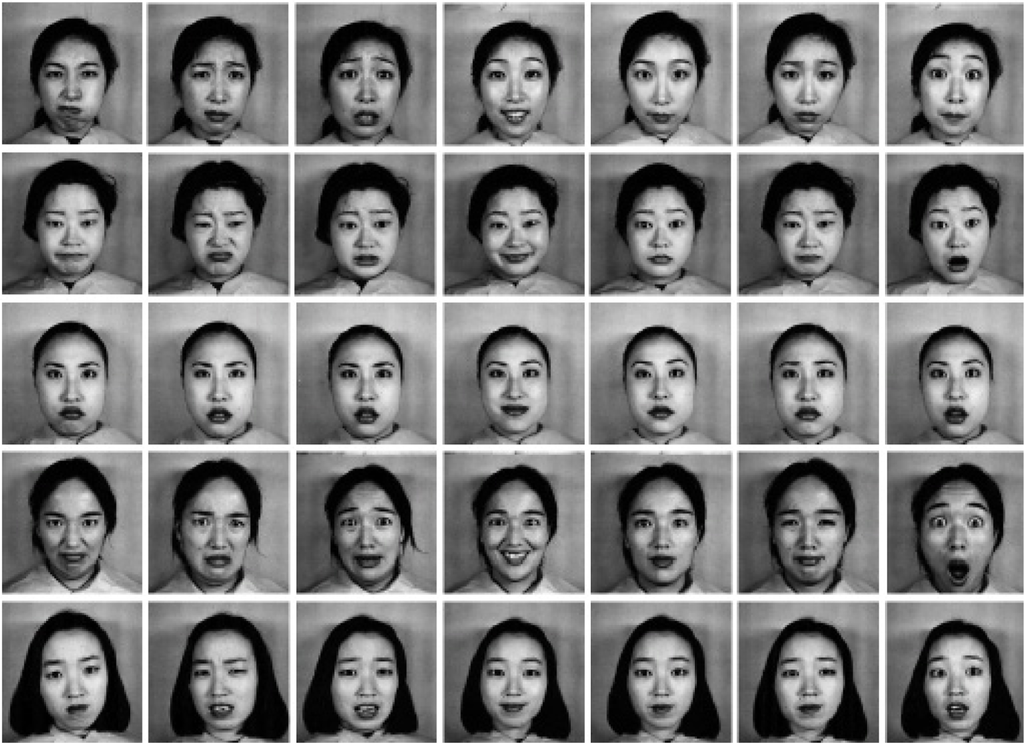
\includegraphics[width=.8\textwidth]{Figures/Chapter4_Jaffe.png} 
  \caption{Ejemplo de la base de datos (JAFFE).}
\end{figure}

\pagebreak
\subsection{Proyección sobre un espacio de dimensión 20}

\underline{\textbf{1) Cotas para $\rho^*$}}

Al igual que el ejemplo de MNIST, se ejemplificará la segunda cota presentada en el capítulo 2. Para esto se calcularon los eigenvalores de la matriz intraclase (B) y de la matriz entre clases (A). Los 20 eigenvalores más grandes y más pequeños de la primera son: \footnote{los eigenvalores menores a $1e^{-10}$ se consideraron numéricamente como 0}

\begin{center}
\begin{tabular}{ | c | c|  c |c | c|  c |c | c|  c |c | c | c|  c |c | c|  c |c | c|  c |c |} 
\hline
5303 & 4627 & 2083 & 1556 & 1370 & 1177 & 851 & 781 & 740 & 705 \\
629 & 596 & 562 & 520 & 498 & 466 & 453 & 403 & 397 & 382 \\
\hline
\hline
\end{tabular}
\end{center}

\begin{center}
\begin{tabular}{ | c | c|  c |c | c|  c |c | c|  c |c | c | c|  c |c | c|  c |c | c|  c |c |} 
\hline
250 & 245 & 231 & 223 & 219 & 203 & 198 & 192 & 176 & 147 \\
141 & 0 & 0 & 0 & 0 & 0 & 0 & 0 & 0 & 0 \\
\hline
\hline
\end{tabular}
\end{center}

De la misma manera, se calculan los 9 eigenvalores más grandes de la matriz entre clases (Los demás son 0):

\begin{center}
\begin{tabular}{ | c | c|  c |c | c|  c |c | c|  c |} 
\hline
14051 & 12922 & 7775 & 3247 & 3138 & 2849 & 1918 & 1336 & 1317 \\
\hline
\hline
\end{tabular}
\end{center}

Usando las formulas del capítulo 2, se tienen las siguientes cotas para $\rho^*$:

\begin{equation*}
\frac{\sum_{i = 1}^{p}\lambda_{A_i}}{\sum_{i = 1}^{p}\lambda_{B_i}} \leq \rho^* \leq \frac{\sum_{i = 1}^{p}\lambda_{(A)_i}}{\sum_{i = 1}^{p}\lambda_{(B)_{n-i+1}}}  
\end{equation*}

\begin{equation*}
\frac{48553}{24099} \leq \rho^* \leq \frac{48553}{2225}
\end{equation*}

\begin{equation*}
2.0147 \leq \rho^* \leq 21.8216
\end{equation*}


\pagebreak
\underline{\textbf{2) Valores de $(\rho^*, f(\rho^*))$}}

En la figura 3.7 se observa fácilmente rapidez de convergencia. En esta gráfica se muestra en el eje $y$ la raíz cuadrada de $f(\rho)$. Los criterios de paro se fijaron iguales que el ejemplo pasado (tol: $1e^{-10}$ y menos de 50 iteraciones). Para la base de JAFFE, se encontraron los siguientes resultados:

\begin{center}
\begin{tabular}{ | c | c|  c |} 
\hline
$iter$ & $\rho$ & $f(\rho)$  \\ 
\hline
\hline
1 & $11.88493$ & $6093.742$  \\ 
\hline
2 & $14.33840$ & $80.44169$  \\ 
\hline
3 & $14.37160$ & $.01093739e$  \\ 
\hline
4 & $14.37161$ & $1.873559 e^{-10}$  \\ 
\hline
\hline
\end{tabular}
\end{center}

\begin{figure}[!ht]
  \centering
  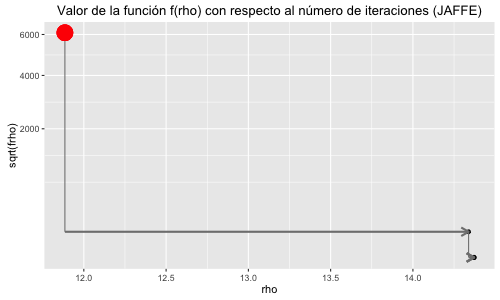
\includegraphics[width=.75 \textwidth]{Figures/Chapter4_Iteraciones_JAF.png} 
  \caption[Valores de $\rho$ y $f(\rho)$ para las iteraciones (JAFFE).]
  {Valores de $\rho$ y $f(\rho)$ para las iteraciones (JAFFE). El punto rojo es el punto inicial. Datos del conjunto de entrenamiento.}
\end{figure}

Se ve que la convergencia cuadrática del método de Newton ayuda a que se alcance el óptimo en pocas iteraciones. En la cuarta iteración $f(\rho)$ ya toma el valor de $1.87 e^{-10}$, muy cercano a 0. 

\pagebreak
\underline{\textbf{3) Datos proyectados en 4 dimensiones}}

De nuevo se maximizó la traza del cociente para un espacio de 20 dimensiones. En la figura 3.8 se muestra como se agrupan los individuos del conjunto de entrenamiento conforme las iteraciones avanzan.

\begin{figure}[!ht]
  \centering
  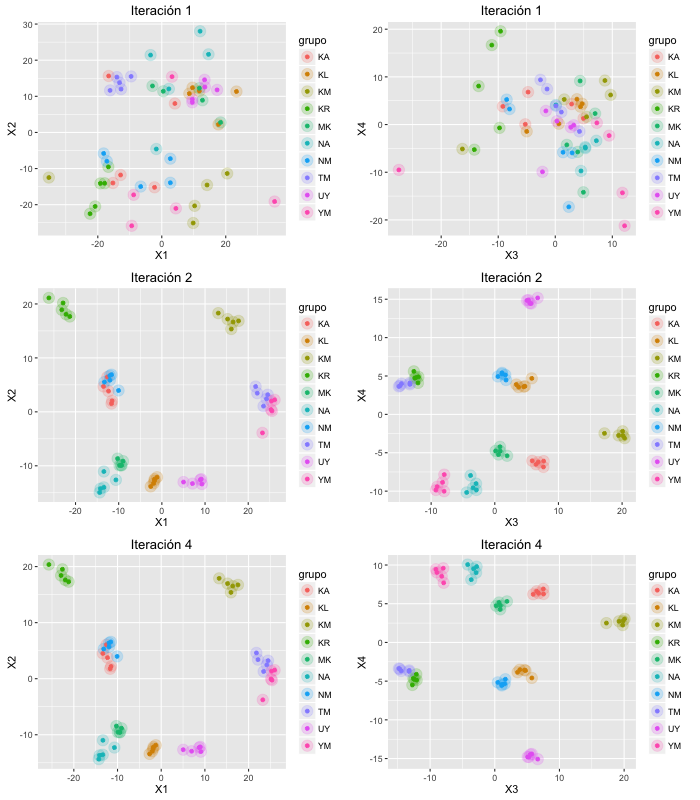
\includegraphics[width=1\textwidth]{Figures/Chapter4_ejemplo20componentes_JAF.png} 
  \caption[Ejemplo de proyección en 20 dimensiones (JAFFE).]
  {Ejemplo de proyección en 20 dimensiones (JAFFE). Las dos imágenes superiores son los datos de entrenamiento proyectadas sobre las 4 primeras componentes tras la primer iteración. Las dos intermedias son en la iteración 3 y las últimas 2 son la última iteración.}
\end{figure}


\subsection{Comparación con otros métodos}

De la misma forma que el ejemplo pasado se compararon los métodos en este caso. Lo único distinto serán las dimensiones a considerar k = 10, 13, 16, 19, 22, 25, 28, 31, 34, 37, 40, 43, 46 y 49. 

\underline{\textbf{1) Tasa de reconocimiento}}

\begin{figure}[!ht]
  \centering
  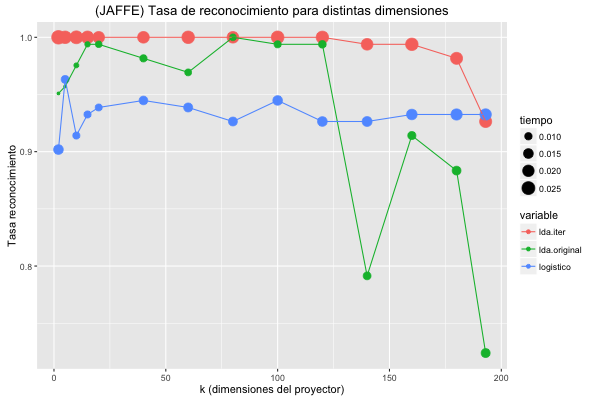
\includegraphics[width=1\textwidth]{Figures/Chapter4_Comparacion_Jaf.png} 
  \caption[Tasa de reconocimiento base (JAFFE)]
  {Tasa de reconocimiento base (JAFFE). En azul se representa el RLM, en verde el ADL y en rojo el método de Newton-Lanczos. En el eje $y$ se muestra la tasa de reconocimiento y en el eje $x$ la dimensión a considerar (k). El tamaño representa el tiempo. Se observa que en el ADL los últimos 4 puntos bajan la predicción. Esto es porque las variables son colineales y al calcular la inversa, causa inestabilidad numérica. Datos del conjunto de entrenamiento.}
\end{figure}

En la figura 3.9 se observa que el método de lda iterativo no tiene ningún error de clasificación para espacios de proyección menor a 40 dimensiones, reduciéndose en espacios de proyección con dimensión más alta. Esto puede deberse a que las últimas componentes son las menos discriminadoras, pero el método de 3-vecinos más cercanos las pondera igual. Una posible modificación que se puede realizar, es ponderar cada componente de acuerdo al poder discriminativo del correspondiente eigenvector.

En la figura 3.10 se muestran las últimas 4 componentes. Se observa que los individuos ya no están tan agrupados como en las primeras 4, por lo que el clasificador de 3-vecinos más cercanos podría no estar funcionando bien para $k > 40$.

\begin{figure}[!ht]
  \centering
  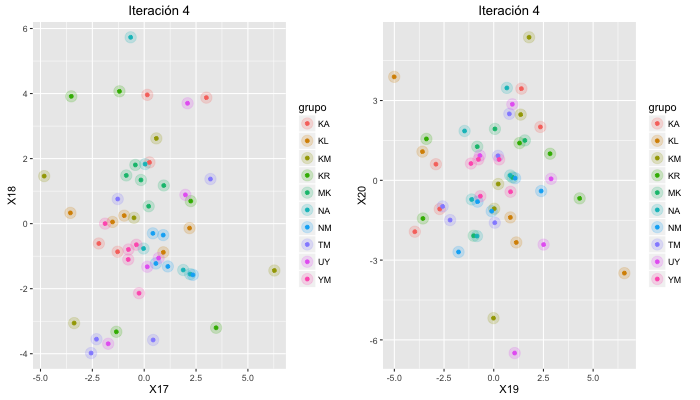
\includegraphics[width=.95\textwidth]{Figures/Chapter4_ultimasComponentes_JAF.png} 
  \caption[Individuos proyectados (JAFFE).]
  {Individuos proyectados (JAFFE). Conjunto de entrenamiento proyectados sobre las ultimas 4 componentes (17,18,19,20). Se observa que los grupos siguen estando relativamente cerca, pero si se toma 3-vecinos más cercanos no necesariamente se escogerá la persona correcta.}
\end{figure}


\underline{\textbf{2) Tiempo de ejecución}}
A continuación, se comparan los tiempos de ejecución de cada método. Para compararlos justamente, se tomaron 3 fases distintas y se comparó solamente el tiempo del modelo.

\begin{itemize}
\item 1) (PCA) Tiempo para calcular los componentes principales del conjunto de entrenamiento
\item 2) (Proyectar) Tiempo para calcular la proyección del conjunto de test
\item 3) (Modelo) Tiempo necesario para hacer las operaciones de cada método

\end{itemize}

\begin{center}
\begin{tabular}{ | c | c |} 
\hline
 PCA(s) & Proyectar(s) \\ 
\hline
\hline
$4.666$ & $4.801$ \\ 
\hline
\hline
\end{tabular}
\end{center}


\begin{center}
\begin{tabular}{ | c | c | c | c ||| c | c | c | c |} 
\hline
Comp & lda.iter & logístico & lda.orig   & Comp & lda.iter & logístico & lda.orig   \\ 
\hline
\hline
$10$ & $0.0352$ & $0.0098$ & $0.0068$ & $31$ & $0.0312$ & $0.0436$ & $0.0136$ \\
$13$ & $0.0324$ & $0.0146$ & $0.0074$ & $34$ & $0.0314$ & $0.0176$ & $0.0134$ \\
$16$ & $0.0378$ & $0.018$ & $0.0082$ & $37$ & $0.0314$ & $0.0224$ & $0.0144$ \\
$19$ & $0.031$ & $0.0114$ & $0.0104$ & $40$  & $0.0312$ & $0.0266$ & $0.0152$ \\
$22$ & $0.0308$ & $0.0128$ & $0.0112$ & $43$ & $0.0294$ & $0.0248$ & $0.0164$ \\
$25$ & $0.0326$ & $0.0136$ & $0.0102$ & $46$ & $0.03$ & $0.0228$ & $0.0188$ \\
$28$ & $0.0318$ & $0.0158$ & $0.0112$ & $49$ & $0.0204$ & $0.0594$ & $0.0176$ \\
\hline
\hline
\end{tabular}
\end{center}

El tiempo está en segundos (s).

Para cada iteración del método de Newton-Lanczos, se calcularon todos los eigenvalores (Excepto si el número de eigenpares a calcular es menor al 5\% del total) ya que al no calcular todos, solo se tendrá una aproximación a sus valores y sus eigenvectores. Por este motivo, se decidió sacrificar tiempo de cómputo por precisión.




	%  \chapter{Conclusiones}
\label{ch:conclusion}

% Párrafo intro 
En este trabajo se expone la técnica de optimización de Newton-Lanczos aplicada al problema de aprendizaje supervisado del Análisis Discriminante Lineal de Fisher (ADLF). El ADLF busca encontrar la mejor matriz de proyección que maximice el cociente de trazas, logrando que los individuos de una misma clase sean proyectados lo más cercano posible entre ellos y lo más separado posible de otra clase. Anteriormente, la solución era considera computacionalmente costosa de resolver; sin embargo, en la actualidad se puede aprovechar la velocidad de convergencia del método de Newton y la rapidez del algoritmo de Lanczos para calcular eigenpares. 

% ------ primero

El método de Lanczos es muy efectivo para calcular solamente algunos de los eigenpares de las matrices. Bajo el contexto de aritmética inexacta, Lanczos implementado con reortogonalización completa resulta ser más eficiente que la factorización SVD, cuando se desea calcular menos del 5 \% de los eigenpares. Aunque este número parece ser demasiado pequeño resulta de gran utilidad; por ejemplo, si la matriz tiene dimensión de $1000 \times 1000$, tener 50 eigenpares podría ser adecuado para el problema. 

\newpage
En este trabajo de tesis se comparó el método ADLF vía Newton-Lanczos con el Análisis Discriminante Lineal (ADL) y la técnica de Regresión Lineal Múltiple (RLM). La comparación se realizó empleando las bases JAFFE y MNIST. Los resultados obtenidos con ADLF vía Newton-Lanczos tuvieron un desempeño similar en comparación con los otros métodos en términos de tasa de reconocimiento y tiempo de cómputo.

Las conclusiones más relevantes de esta tesis son las siguientes:

\begin{itemize}
\item Se implementó computacionalmente una técnica de optimización que anteriormente resultaba difícil de resolver.
\item Una de las principales ventajas de esta metodología es que no requiere ningún supuesto sobre la distribución de los datos.
\item Se evaluó el desempeño de esta metodología con respecto a técnicas conocidas y los resultados fueron satisfactorios.
\item Se realizaron dos pruebas diferentes y se obtuvo que en algunos casos el ADLF vía Newton-Lanczos tuvo una precisión mayor con respecto a los otros dos métodos.
\end{itemize}


% ------ Tercero
Una de las complicaciones del algoritmo de Lanczos es la reortogonalización de la base. En este estudio se utilizó el método de reortogonalización completa; sin embargo, existen modificaciones al algoritmo que pueden ser exploradas con el objetivo de lograr mayor eficiencia en términos computacionales. Por ejemplo, J.W. Demmel (1997) \cite{demmel1997applied} propone algunas alternativas que pueden ser utilizadas para mejorar el proceso de reortogonalización de la base en el algoritmo de Lanczos.




		
	% \appendix
	%  \chapter{Apéndice A: Optimización de $Tr(V^TA V)$}
\label{ch:appendixA}


Sea $A \in {\rm I\!R}^{nxn}$ una matriz simétrica cuya factorización espectral es:

\begin{equation*}
\begin{aligned}
	A =& U^T \Lambda U \qquad U^T U = I_n\\
	\Lambda =& diag(\lambda_{A_1}, ..., \lambda_{A_n} )
\end{aligned}
\end{equation*}

donde $\lambda_{A_1} \geq \lambda_{A_2} \geq ... \geq \lambda_{A_n}$ son los valores propios de $A$ y $U$ una matriz ortogonal. En este apéndice se demostrará que:

\begin{equation}\label{A1:1}
\begin{aligned}
\max_{\substack{V^T V = I \\V \in {\rm I\!R}^{nxp} }}Tr(V^T A V) = \lambda_{A_1} + \lambda_{A_2} + ... + \lambda_{A_p}
\end{aligned}
\end{equation}

\section{Problema relajado}
Sean $\mathcal{U}_p$ y $\mathcal{V}_p$ dos conjuntos de matrices en ${\rm I\!R}^{nxp}$ tales que:

\begin{equation*}
\begin{aligned}
\mathcal{U}_p =& \{V \in {\rm I\!R}^{nxp} | V^TV = I_p\}	\\
\mathcal{V}_p =& \{V \in {\rm I\!R}^{nxp} | diag(V^TV) = I_p\}	
\end{aligned}
\end{equation*}

El conjunto $\mathcal{V}_p$ contiene a todas las matrices donde que cada columna tiene norma euclidiana igual a 1.

\begin{lemma}
El conjunto $\mathcal{V}_p$ es compacto en ${\rm I\!R}^{nxp}$
\begin{proof}
Por definición, si $V \in \mathcal{V}_p$ entonces $||V||_F = \sqrt(p)$.
Más aún, $\mathcal{V}_p$ contiene todos sus puntos límite.
\end{proof}
\end{lemma}

Si se relaja el problema original como:
\begin{equation} \label{A1:2}
	\max_{V \in \mathcal{V}_p} Tr(V^T A V)
\end{equation}
Como $\mathcal{V}_p$ es un conjunto compacto, la función continua $Tr(V^T AV)$ alcanza su valor máximo (o mínimo) en este conjunto. Ahora, como $\mathcal{U}_p \subset \mathcal{V}_p$, se tiene inmediatamente la desigualdad:

\begin{equation} \label{A1:3}
\max_{V \in \mathcal{U}_p} Tr(V^T A V) \leq \max_{V \in \mathcal{V}_p} Tr(V^T AV)	
\end{equation}

Por lo tanto, se se procede a establecer el siguiente resultado:

\begin{theorem}\label{A1:T1}
\begin{equation*}
	\max_{V \in \mathcal{V}_p} Tr(V^T A V) = \lambda_{A_1} + \lambda_{A_2} + ... + \lambda_{A_p}
\end{equation*}
\end{theorem}

\begin{proof}
Para $V \in \mathcal{V}_p$ con $V = (v_1 \enskip v_2 \enskip ...\enskip v_p)$ y $v_j$ la j-ésima columna de $V$. Se define el vector:

\begin{equation*}
	\mathbf{v} = (v_1^T\enskip v_2^T \enskip...\enskip v_p^T)^T \enskip \in \enskip {\rm I\!R}^{np}
\end{equation*}

o lo que es equivalente:
\begin{equation*}
\mathbf{v} = \left(\!
    \begin{array}{c}
		v_1 \\
		v_2 \\
		\vdots \\
		v_p \\
\end{array}
  \!\right) \quad
\end{equation*}

Entonces la $Tr(V^TAV) = v_1^TAv_1 + v_2^TAv_2 + ... + v_p^TAv_p$ y el problema \ref{A1:2} puede ser formulado como sigue:

\begin{equation} \label{A1:4}
	\max_{\substack{\mathbf{v}^T \mathbb{B}_j \mathbf{v} = 1 \\ j = 1, ..., p}} \mathbf{v}^T\mathbb{A} \mathbf{v}
\end{equation}

con las matrices $\mathbb{A}$ y $\mathbb{B}_j$:


\begin{equation*}
\mathbb{A} = \left(\!
    \begin{array}{cccccc}
		A & 0 & \hdots & 0 & \hdots & 0 \\
		0 & A & \hdots & 0 & \hdots & 0 \\
		\vdots & \vdots & \vdots & \vdots & \vdots & \vdots \\
		0 & 0 &  \hdots & A & \hdots & 0 \\
		\vdots & \vdots & \vdots & \vdots & \vdots & \vdots \\
		0 & 0 & \hdots & 0 & \hdots & A \\
\end{array}
  \!\right) \quad
\end{equation*}


\begin{equation*}
\mathbb{B}_j = \left(\!
    \begin{array}{cccccc}
		0 & 0 & \hdots & 0 & \hdots & 0 \\
		0 & 0 & \hdots & 0 & \hdots & 0 \\
		\vdots & \vdots & \vdots & \vdots & \vdots & \vdots \\
		0 & 0 &  \hdots & I_n & \hdots & 0 \\
		\vdots & \vdots & \vdots & \vdots & \vdots & \vdots \\
		0 & 0 & \hdots & 0 & \hdots & 0 \\
\end{array}
  \!\right) \quad
\end{equation*}

En ambas matrices hay $p$ bloques en los renglones y $p$ bloques en las columnas. Para $\mathbb{B}_j$ el bloque $(j,j)$ es $I_n$ y todos los demás son matrices cero. De esta manera, la función lagrangiana asociada al problema es:

\begin{equation*}
\mathcal{L}_j(\mathbf{v}, \eta) = \mathbf{v}^T \mathbb{A} \mathbf{v} - \sum\limits_{j=1}^{p}(\eta_j(\mathbf{v}^T\mathbb{B}_j\mathbf{v}-1))
\end{equation*}

Las condiciones de primer orden para la solución óptima son (considerando que $A$ es simétrica:
\begin{equation}\label{A1:5}
\begin{aligned}
	\nabla_{\mathbf{v}} \mathcal{L}(\mathbf{v}, \eta) =& \quad 2 \mathbb{A}\mathbf{v} - 2 \sum\limits_{j=1}^p (\eta_j(\mathbf{v}^T \mathbb{B}_j \mathbf{v})) = \quad 0 \\
	\nabla_{\eta_j} \mathcal{L}(\mathbf{v}, \eta)  =& \quad \mathbf{v}^T \mathbb{B}_j \mathbf{v} = 1 \quad con \quad j = 1, ...,p 
\end{aligned}
\end{equation}

De la primera ecuación de \ref{A1:5}, se tiene que:

\begin{equation*}
	\left(\mathbb{A}-\sum\limits_{j=1}^p \eta_j \mathbb{B}_j \right) v = 0
\end{equation*}

Donde la matriz $(\mathbb{A}-\sum\limits_{j=1}^p \eta_j \mathbb{B}_j)$ es diagonal a bloques. De hecho, el bloque $(j,j)$ es:

\begin{equation*}
(A-\eta_j I_n)v_j = 0 \quad \Rightarrow \quad Av_j = \eta_j v_j	
\end{equation*}

Entonces, $\eta_j$ debe ser un eigenvalor de A y $v_j$ su correspondiente eigenvector. Tomando de nuevo la ecuación de arriba, y multiplicándola por $v^T$ se obtiene:

\begin{equation*}
v^T \mathbb{A}v = \sum\limits_{j=1}^p (\eta_j)(v^T \mathbb{B}_j v)	
\end{equation*}

Ahora, usando la segunda ecuación de \ref{A1:5}, se tiene que:

\begin{equation*}
	v^T \mathbb{A}v = \sum\limits_{j=1}^p \eta_j
\end{equation*}

Por lo tanto, con el fin de maximizar la función $v^T \mathbb{A} v$ en $\mathcal{V}_p$, se deben escoger los primeros $p$ eigenvalores de la matriz A. Esto es:

\begin{equation*}
	\eta_j = \lambda_{A_j}, \qquad j = 1, ..., p
\end{equation*}

\end{proof}


Ahora, se tienen todas las piezas para demostrar el resultado principal.


\begin{theorem}\label{A1:T2}
\begin{equation*}
\max_{\substack{V^TV= I_p \\V \in {\rm I\!R}^{nxp}}} Tr(V^T A V)	= \lambda_{A_1} + \lambda_{A_2} + ... +\lambda_{A_p}
\end{equation*}
\end{theorem}

\begin{proof}
Se ha mostrado que:
\begin{equation*}
\max_{V \in \mathcal{U}_p} Tr(V^T A V)	\leq \lambda_{A_1} + \lambda_{A_2} + ... +\lambda_{A_p}	
\end{equation*}
\end{proof}

Considerando la matrix $U \in {\rm I\!R}^{nxn}$ de la factorización espectral de A, tal que $U = (u_1 \enskip u_2 \enskip ... \enskip u_n)$. Tomando las primeras $p$ columnas de $U$ se define $U^*$:



\begin{equation*}
\begin{aligned}
    U^* =& (u_1 \enskip u_2\enskip ...\enskip u_p) \quad con \quad U^* \in \mathcal{U}_p \quad y \\
	Tr(U^* A U) =& \lambda_{A_1} + \lambda_{A_2} + ... + \lambda_{A_p}
\end{aligned}
\end{equation*}



\section{Observaciones finales}

Se toman los resultados de la sección anterior para hacer las siguientes observaciones:


\begin{remark}
Se puede extender el último teorema, usando el mismo conjunto $\mathcal{V}_p$ y cambiando la maximización a minimización para obtener que:

\begin{equation}\label{A1:6}
\min_{V \in \mathcal{U}_p} Tr(V^T A V)	= \lambda_{A_n} + \lambda_{A_{n-1}} + ... +\lambda_{A_{n-(p-1)}}
\end{equation}
\end{remark}


\begin{remark}
Cuando $p = 1$, se pueden obtener las bien conocidas propiedades del cociente de Raleigh:

\begin{equation}\label{A1:7}
\begin{aligned}
\left(\min_{v^vv = 1} v^T A v	\right)=& \lambda_{A_n} \\
\left(\max_{v^vv = 1} v^T A v	\right)=& \lambda_{A_1}
\end{aligned}
\end{equation}
\end{remark}





	% \chapter{Apéndice B: Códigos en R}
\label{ch:appendixB}

\section{Experimentos numéricos}
\subsection{$01\_Prueba20comp$}

\begin{lstlisting}[language=R, basicstyle=\small]
library(ProjectTemplate)
reload.project()

# Jaffe.20 & Mnist.20  are 5 element lists:
# 1) iterative model
# 2) data frame with \rho, f\rho values
# 3) projection matrix V
# 4) test error
# 5) knn model

Jaffe.20 <- prueba.20comp(JAFFE.train, JAFFE.test, "JAFFE")
Mnist.20 <- prueba.20comp(MNIST.train, MNIST.test, "MNIST")

Jaffe.20$modelo.iterativo
Mnist.20$modelo.iterativo
\end{lstlisting}

\subsection{$02\_Models\_comparisons$}
\begin{lstlisting}[language=R, basicstyle=\small]
# 1) Data y proyeccion size --------------------------------
library(ProjectTemplate)
reload.project()

numComp.Jaffe <- c(10,13,16,19,22,25,28,31,
                   34,37,40,43,46,49) 
numComp.Mnist <- c(2,5,10,15,20,40,60,80,
                   100,120,140,160,180,193)

comp.error.MNIST<-comparacion.modelos(train.p = MNIST.train,
                                 test.p = MNIST.test, 
                                 dataset = "MNIST", 
                                 numComp = numComp.Mnist,
                                 fortran = FALSE)

comp.error.JAFFE<-comparacion.modelos(train.p = JAFFE.train,
                                  test.p = JAFFE.test, 
                                  dataset = "JAFFE", 
                                  numComp = numComp.Jaffe,
                                  fortran = FALSE)
# 2) Graphs ------------------------------------------------

graficar.comparacion(datos = comp.error.MNIST, 
                     numComp = numComp.Mnist, 
                     label = "MNIST")

graficar.comparacion(datos = comp.error.JAFFE, 
                     numComp = numComp.Jaffe, 
                     label = "JAFFE")
\end{lstlisting}

\subsection{$03\_Profiling$}
\begin{lstlisting}[language=R, basicstyle=\small]
# 1) Data y proyeccion size --------------------------------
library(ProjectTemplate)
reload.project()

# 1) Componentes ------------------------------------------
numComp.Jaffe <- c(10,13,16,19,22,25,28,31,
                   34,37,40,43,46,49) 
numComp.Mnist <- c(2,5,10,15,20,40,60,80,
                   100,120,140,160,180,193)
# 2) Profiling ----------------------------------------
prof.Mnist <- prolifiling.model(train.p = MNIST.train, 
                                test.p = MNIST.test,
                                dataset = "MNIST",
                                numComp = numComp.Mnist)
prof.Jaffe <- prolifiling.model(train.p = JAFFE.train, 
                                test.p = JAFFE.test,
                                dataset = "JAFFE",
                                numComp = numComp.Jaffe)

# 3) Graphs -------------------------------------------
graficar.profiling(times.profiling = prof.Mnist, 
                   numComp = numComp.Mnist, 
                   dataset = "MNIST")
graficar.profiling(times.profiling = prof.Jaffe, 
                   numComp = numComp.Jaffe, 
                   dataset = "JAFFE")
\end{lstlisting}

\section{Funciones}
\subsection{$load\_libraries$}
\begin{lstlisting}[language=R, basicstyle=\small]
# 1) Load libraries ----------------------------------------
set.seed(12345)
library(plyr) # Tools for split, applying and combine data
library(dplyr) # package of grammar of data manipulation
library(tidyr) # package to efficiently "tidy" data
library(FactoMineR) # Package for multivariate analysis
library(ggplot2) # Graphing package "Grammar of Graphics"
library(gridExtra) # Package to work with grid graphics
library(class) # Functions for classification, including knn
library(nnet) # Software for multinomial linear models
library(MASS) # "Applied Statistics with S"



# 1) Fisher eficiente ---------------------------------
lda.iter.ef <- function (test.p, 
                         train.p, 
                         espacio.proy,
                         prior = proportions,
                         tol = 1e-10) {
  
  # Prepare matrix of data
  x <- train.p %>% dplyr::select(-grupo)
  x <- as.matrix(x)
  
  # Get dimensions
  n <- nrow(x)
  p <- ncol(x)
  
  # Get number of groups and the levels
  g <- as.factor(train.p$grupo)
  lev <- lev1 <- levels(g)
  
  # Get the number of images per class
  counts <- as.vector(table(g))
  proportions <- counts/n
  ng <- length(proportions)
  names(prior) <- names(counts) <- lev1
  
  # Group means and total mean
  group.means <- tapply(c(x), list(rep(g, p), col(x)), mean)
  all.means <- as.matrix(colMeans(x)) %>% t()
  
  # Scatter Matrices 
  #Intra class
  B <- t(x - group.means[g, ]) %*% (x - group.means[g, ]) 
  # Between class
  A <- (t(group.means)-matrix(rep(all.means,10),ncol=10))%*% 
    diag(counts) %*% 
    t(t(group.means)-matrix(rep(all.means,10),ncol=10)) 
  
  # Initialization
  rhoAnt = -1000000
  iter=1
  dimension = espacio.proy
  # rho = (cota.inf + cota.sup)/2
  rho = 0
  frho = sum(eigen(A-rho*B)$values[1:dimension])
  V = eigen(A-rhoAnt*B)$vectors[,(1:dimension)]
  
  # list of results
  a=list()
  a[[1]] <- list(iter = 1, rho = rho, frho = frho, V = V) 
  
  # Iterative method (use of efficient irlba method)
  while(iter < 50 & abs(rho-rhoAnt)>tol){
    print(paste("iteracion: ",as.character(iter)))
    rhoAnt = rho
    iter=iter+1  
    V = eigen(A-rhoAnt*B)$vectors[,(1:dimension)] # Lanczos
    rho = sum(diag(t(V) %*% A %*% V)) /
    sum(diag(t(V) %*% B %*% V))
    frho = sum(eigen(A-rho*B)$values[1:dimension])
    a[[iter]] <- list(iter = iter, rho = rho,
                      frho = frho, V = V)
  }
  
  # Getting the projection matrix
  scaling <- V
  dimnames(group.means)[[2L]] <- colnames(x)
  cl <- match.call()
  cl[[1L]] <- as.name("lda.iter")
  structure(list(iteraciones = a, 
                 prior = prior, 
                 counts = counts, 
                 means = group.means, 
                 scaling = scaling, 
                 lev = lev, 
                 N = n, 
                 call = cl, 
                 class = "lda.iter"))
}

# 2) Fisher para pruebas ------------------------------
lda.iter <- function (test.p, 
                      train.p, 
                      espacio.proy,
                      prior = proportions, 
                      tol = 1e-10) {
  
  # Prepare matrix of data
  x <- train.p %>% dplyr::select(-grupo) %>% as.matrix()
  
  # Get dimensions
  n <- nrow(x)
  p <- ncol(x)
  
  # Get number of groups and the levels
  g <- as.factor(train.p$grupo)
  lev <- lev1 <- levels(g)
  
  # Get the number of images per class
  counts <- as.vector(table(g))
  proportions <- counts/n
  ng <- length(proportions)
  names(prior) <- names(counts) <- lev1
  
  # Group means and total mean
  group.means <- tapply(c(x), list(rep(g, p), col(x)), mean)
  all.means <- as.matrix(colMeans(x)) %>% t()
  
  # Scatter Matrices 
  #Intra class
  B <- t(x - group.means[g, ]) %*% (x - group.means[g, ]) 
  # Between class
  A <- (t(group.means)-matrix(rep(all.means,10),ncol=10))%*% 
    diag(counts) %*% 
    t(t(group.means)-matrix(rep(all.means,10),ncol=10)) 
  
  # [not run] Intra class + Between class = Total variance
  diag(A+B) 
  diag(49*(as.matrix(x) %>% cov))
  
  # [not run] EigenValues Time
  (eigen(B))$values
  (eigen(A))$values
  
  # [not run] Boundaries
  cota.inf <- sum((eigen(A))$values[1:espacio.proy])/
    sum((eigen(B))$values[1:espacio.proy])
  cota.sup <- sum((eigen(A))$values[1:espacio.proy])/
sum((eigen(B))$values[(dim(A)[1]+1-espacio.proy):dim(A)[1]])
  
  # Initialization
  rhoAnt = -1000000
  iter=1
  dimension = espacio.proy
  rho = (cota.inf + cota.sup)/2
  
  frho = sum(eigen(A-rho*B)$values[1:dimension])
  V = eigen(A-rhoAnt*B)$vectors[,(1:dimension)]
  
  # list of results
  a=list()
  a[[1]] <- list(iter = 1, rho = rho, frho = frho, V = V) 
  
  # Iterative method (use of efficient irlba method)  
  while(iter < 50 & abs(rho-rhoAnt)>tol){
    print(paste("iteracion: ",as.character(iter)))
    rhoAnt = rho
    iter=iter+1  
    V = eigen(A-rhoAnt*B)$vectors[,(1:dimension)]
rho = sum(diag(t(V)%*%A %*% V)) /sum(diag(t(V) %*% B %*% V))
    frho = sum(eigen(A-rho*B)$values[1:dimension])
a[[iter]] <-list(iter = iter, rho = rho, frho = frho, V = V)
  }
  
  # Getting the projection matrix
  scaling <- V
  dimnames(group.means)[[2L]] <- colnames(x)
  cl <- match.call()
  cl[[1L]] <- as.name("lda.iter")
  structure(list(iteraciones = a, 
                 prior = prior, 
                 counts = counts, 
                 means = group.means, 
                 scaling = scaling, 
                 lev = lev, 
                 N = n, 
                 call = cl, 
                 cota.inf = cota.inf, 
                 cota.sup = cota.sup, 
                 class = "lda.iter"))
}

# 3) LDA original -------------------------------------
lda.original <- function (x, 
                          grouping, 
                          prior = proportions, 
                          tol = 1e-04, 
                          nu = 5) {
  
  # Prepare matrix of data
  x <- as.matrix(x)
  n <- nrow(x)
  
  # Get dimensions
  p <- ncol(x)
  g <- as.factor(grouping)
  
  # Get number of groups and the levels
  lev <- lev1 <- levels(g)
  counts <- as.vector(table(g))
  
  # Get the number of images per class
  proportions <- counts/n
  ng <- length(proportions)
  names(prior) <- names(counts) <- lev1
  
  # Group means 
  group.means <- tapply(c(x), list(rep(g, p), col(x)), mean)
  f1 <- sqrt(diag(var(x - group.means[g, ])))
  scaling <- diag(1/f1, , p)
  
  # Calculate and project
  fac <-  1/(n - ng)
  X <- sqrt(fac) * (x - group.means[g, ]) %*% scaling
  X.s <- svd(X, nu = 0L)
  rank <- sum(X.s$d > tol)
  scaling <- scaling %*% X.s$v[, 1L:rank] %*% 
    diag(1/X.s$d[1L:rank], , rank)
  xbar <- colSums(prior %*% group.means)
  fac <-1/(ng - 1)
  X <- sqrt((n * prior) * fac) * scale(group.means, 
        center = xbar, scale = FALSE) %*% scaling
  X.s <- svd(X, nu = 0L)
  rank <- sum(X.s$d > tol * X.s$d[1L])
  scaling <- scaling %*% X.s$v[, 1L:rank]
  
  # Export
  dimnames(scaling) <- list(colnames(x), paste("LD",
          1L:rank, sep = ""))
  dimnames(group.means)[[2L]] <- colnames(x)
  cl <- match.call()
  cl[[1L]] <- as.name("lda")
  structure(list(prior = prior, counts = counts, 
                 means = group.means, 
                 scaling = scaling, lev = lev, 
                 svd = X.s$d[1L:rank], N = n, 
                 call = cl), class = "lda")
}

# 4) Lanczos Fortran -----------------------------------
# Give r0, A
lanczos.iter <- function(A){
  Dim = dim(A)[2]
  r0 = matrix(rep(0,Dim), ncol = 1)
  for(i in 1:Dim){
    r0[i] = runif(1, 0, 1) 
  }
r0 = r0 / sqrt(sum(r0^2))
r = list()
b = list()
a = list()
q = list()

q[[1]] = 0 # q0
r[[1]] = r0 #r0
b[[1]] = sqrt(sum(r[[1]]^2)) # b1
q[[2]] = as.matrix(r[[1]]/b[[1]], ncol =D) #q1
a[[1]] = t(q[[2]]) %*% A %*% q[[2]] #a1
q[[1]]
j <- 2
q = cbind(q[[1]], q[[2]])
while(b[[j-1]] > .0000001 | j < Dim+1){
  z = A %*% q[,j]
  z = z - q %*% (t(q) %*% z)
  z = z - q %*% (t(q) %*% z)
  b[[j]] = sqrt(sum(z^2))
  q.temp = z/b[[j]]
  q <- cbind(q, q.temp)
  a[[j]] = t(q[,j+1]) %*% A %*% q[,j+1]
  j = j+1
  print(j)
}

dyn.load("/usr/lib/liblapack.dylib")

Jobz <- as.character('V')#Get The eigenval and Eigenvector
N <- as.integer(Dim)#Matrix Dimension
D <- unlist(a)[1:Dim]#Diagonal
E <- unlist(b)[2:(Dim)]#Upper (and lower) diagonal
Z <- array(0.0,N*N)#storage for eigenvectors
Ldz <- N#Leading dimension of Z (in our case number of rows)
Work <- array(0.0,2*N)#Storage for processing
info <- as.integer(0)#Info flag

res<-.Fortran("dstev", Jobz, N, D, E, Z, Ldz, Work, info)

evalues <- res[[3]]
evectors <- matrix(res[[5]],N,N)
list(evalues, evectors)
}

# 5) Fisher eficiente ---------------------------------
lda.iter.fortran<- function (test.p = test.p, 
                         train.p = train.p, 
                         espacio.proy,
                         prior = proportions,
                         tol = 1e-10) {
  
  # Prepare matrix of data
  x <- train.p %>% dplyr::select(-grupo)
  x <- as.matrix(x)
  
  # Get dimensions
  n <- nrow(x)
  p <- ncol(x)
  
  # Get number of groups and the levels
  g <- as.factor(train.p$grupo)
  lev <- lev1 <- levels(g)
  
  # Get the number of images per class
  counts <- as.vector(table(g))
  proportions <- counts/n
  ng <- length(proportions)
  names(prior) <- names(counts) <- lev1
  
  # Group means and total mean
  group.means <- tapply(c(x), list(rep(g, p), col(x)), mean)
  all.means <- as.matrix(colMeans(x)) %>% t()
  
  # Scatter Matrices 
  #Intra class
  B <- t(x - group.means[g, ]) %*% (x - group.means[g, ]) 
  # Between class
  A <- (t(group.means)-matrix(rep(all.means,10),ncol=10))%*% 
    diag(counts) %*% 
    t(t(group.means)-matrix(rep(all.means,10),ncol=10)) 
  
  # Initialization
  rhoAnt = -1000000
  iter=1
  dimension = espacio.proy
  # rho = (cota.inf + cota.sup)/2
  rho = 0
  frho = sum(eigen(A-rho*B)$values[1:dimension])
  V = eigen(A-rhoAnt*B)$vectors[,(1:dimension)]
  
  # list of results
  a=list()
  a[[1]] <- list(iter = 1, rho = rho, frho = frho, V = V) 
  
  # Iterative method (use of efficient irlba method)
  while(iter < 50 & abs(rho-rhoAnt)>tol){
    print(paste("iteracion: ",as.character(iter)))
    rhoAnt = rho
    iter=iter+1  
    
  V = lanczos.iter(A-rhoAnt*B)[[2]][,(1:dimension)]#Lanczos
    rho = sum(diag(t(V) %*% A %*% V)) /
      sum(diag(t(V) %*% B %*% V))
    frho = sum(lanczos.iter(A-rhoAnt*B)[[1]][1:dimension])
    a[[iter]] <- list(iter = iter, rho = rho,
                      frho = frho, V = V)
  }
  
  # Getting the projection matrix
  scaling <- V
  dimnames(group.means)[[2L]] <- colnames(x)
  cl <- match.call()
  cl[[1L]] <- as.name("lda.iter")
  structure(list(iteraciones = a, 
                 prior = prior, 
                 counts = counts, 
                 means = group.means, 
                 scaling = scaling, 
                 lev = lev, 
                 N = n, 
                 call = cl, 
                 class = "lda.iter"))
}
\end{lstlisting}

\subsection{$functions\_comparison$}
\begin{lstlisting}[language=R, basicstyle=\small]
comparacion.modelos <- function(train.p, test.p, 
                                dataset,numComp, 
                                fortran = FALSE){
  # lda iterativo
  print(paste("===Corriendo el modelo con la base",dataset))
  
  lda.iter <- sapply(1:14, function(x){
    print(paste("Iteracion con: ", 
                numComp[x], 
                " componentes."))
    
    # Run model with different number of components
    if(fortran == FALSE){
    modelo.iterativo <- lda.iter.ef(train.p = train.p, 
                                    test.p = test.p, 
                                  espacio.proy = numComp[x])
    }else{
      modelo.iterativo <- lda.iter.fortran(train.p = train.p, 
                                      test.p = test.p, 
                                  espacio.proy = numComp[x])
    }
    # Data.frame with information of  (\rho and f(\rho))
    iter <- sapply(1:length(modelo.iterativo$iteraciones), 
                   function(x){
          data.frame(modelo.iterativo$iteraciones[[x]]$rho,
                  modelo.iterativo$iteraciones[[x]]$frho)%>% 
                setNames(c("rho", "frho")) %>% data.frame()
                   }) %>% t() %>% data.frame() %>% 
      mutate(iter = 1:nrow(.), 
             rho = unlist(rho),
             frho = unlist(frho))
    iter <- iter %>% data.frame() %>% 
      dplyr::mutate(frho2 = c(iter$frho[2:nrow(.)],NA ),
                    rho2 = c(iter$rho[2:nrow(.)], NA))
    
    # Projected data into a 20-dimensional space
    V <- modelo.iterativo$iteraciones[[
      length(modelo.iterativo$iteraciones)]]$V
    
    train.proyectados <- data.frame(as.matrix(train.p %>% 
                          dplyr::select(-grupo)) %*% V) %>%
      mutate(grupo = train.p$grupo)
    
    test.proyectados <- data.frame(as.matrix(test.p %>% 
                          dplyr::select(-grupo)) %*% V) %>%
      mutate(grupo = test.p$grupo)
    
    # K-nn model
    
    print("Iniciando modelo knn")
  modelo <- knn(train = train.proyectados[,c(1:numComp[x])], 
                test = test.proyectados[, c(1:numComp[x])], 
                  cl = train.proyectados$grupo, k = 3)
    pred <- data.frame(original = test.proyectados$grupo, 
                       predicho = modelo)
    
    pred <- pred %>% mutate(verdad = original != predicho)
    sum(pred$verdad)/nrow(pred)
  })
  
  modelo.logistico <- lapply(1:14, function(x){
    modelo <- multinom(grupo~., 
          data = train.p[,c(1:numComp[x], dim(train.p)[2])],
                       MaxNWts = 10000)
    predichos <- predict(modelo, 
                         newdata = test.p[,c(1:numComp[x])])
    pred <- data.frame(original = test.p$grupo, 
                       predicho = predichos)
    pred <- pred %>% mutate(verdad = original != predicho)
    sum(pred$verdad)/nrow(pred)
  })
  
  lda.original <- lapply(1:14, function(x){
    modelo<- lda(grupo ~ ., 
                 train.p[,c(1:numComp[x], 
                            dim(train.p)[2])], 
                 prior = c(1,1,1,1,1,1,1,1,1,1)/10)
  predichos <- predict(modelo, test.p[,1:numComp[x]])$class
    pred <- data.frame(original = test.p$grupo, 
                       predicho = predichos)
    pred <- pred %>% mutate(verdad = original != predicho)
    sum(pred$verdad)/nrow(pred)
  })
  
  data.frame(lda.iter = unlist(lda.iter), 
             logistico = unlist(modelo.logistico), 
             lda.original = unlist(lda.original))
}

graficar.comparacion <- function(datos, numComp, label){
  plot1 <- datos %>% 
    #write.table(sep = ';', pipe('pbcopy'), row.names= F)
    mutate(numComp = numComp) %>% 
    gather(variable, value, lda.iter:lda.original) %>% 
    ggplot(aes(x = numComp , y = 1-value, 
      group = factor(variable), color = factor(variable))) +
    geom_point() + geom_line()+
    labs(title = "Tasa de reconocimiento conforme 
         numero el espacio de proyeccion", 
         x = "numero de entrenamiento por grupo", 
         y="tasa reconocimiento")
  
  png(filename =paste(getwd(), "/graphs/Chapter4_comp_", 
        label, ".png", sep =""), width = 600,  height = 400)
  grid.arrange(plot1, ncol =1)
  dev.off()
}
\end{lstlisting}

\subsection{$functions\_prueba20comp$}
\begin{lstlisting}[language=R, basicstyle=\small]
# funciones prueba 20 componentes

plot.comp <- function(V1, label, train.p, test.p){
  train.proyectados <- data.frame(as.matrix(train.p %>% 
                          dplyr::select(-grupo)) %*% V1) %>%
    mutate(grupo = train.p$grupo)
  
  test.proyectados <- data.frame(as.matrix(test.p %>% 
                          dplyr::select(-grupo)) %*% V1) %>%
    mutate(grupo = test.p$grupo)
  
  a1 = ggplot(train.proyectados) + 
    geom_point(aes(x=X1, y=X2, 
                   group = grupo, color = grupo), 
               size=5, alpha = .2) + 
    geom_point(aes(x=X1, y=X2, 
                   group = grupo, color = grupo))+ 
    labs(title = label)
  a2 = ggplot(train.proyectados) + 
    geom_point(aes(x=X3, y=X4, 
                   group = grupo, color = grupo), 
               size=5, alpha = .2) + 
    geom_point(aes(x=X3, y=X4, 
                   group = grupo, color = grupo))+ 
    labs(title = label)
  list(a1,a2)
}
plot.ult <- function(V1, label, train.p, test.p){
  train.proyectados <- data.frame(as.matrix(train.p %>% 
                          dplyr::select(-grupo)) %*% V1) %>%
    mutate(grupo = train.p$grupo)
  
  test.proyectados <- data.frame(as.matrix(test.p %>% 
                          dplyr::select(-grupo)) %*% V1) %>%
    mutate(grupo = test.p$grupo)
  a7 =  ggplot(train.proyectados) + 
    geom_point(aes(x=X17, y=X18, 
                   group = grupo, color = grupo), 
               size=5, alpha = .2) + 
    geom_point(aes(x=X17, y=X18, 
                   group = grupo, color = grupo))+ 
    labs(title = label)
  
  a8 =  ggplot(train.proyectados) + 
    geom_point(aes(x=X19, y=X20, 
                   group = grupo, color = grupo), 
               size=5, alpha = .2) + 
    geom_point(aes(x=X19, y=X20, 
                   group = grupo, color = grupo))+ 
    labs(title = label)
  list(a7,a8)
}
prueba.20comp <- function(train.p, test.p, dataset){
  # Iterative LDA, projected to a 20-dimentional space
  modelo.iterativo <- lda.iter(train.p = train.p, 
                               test.p = test.p,
                               espacio.proy = 20)
  # Data.frame with information of (\rho and f(\rho))
  iter <- sapply(1:length(modelo.iterativo$iteraciones), 
                 function(x){
          data.frame(modelo.iterativo$iteraciones[[x]]$rho,
                modelo.iterativo$iteraciones[[x]]$frho)  %>% 
                     setNames(c("rho", 
                            "frho")) %>% data.frame()}) %>% 
    t() %>% data.frame() %>% 
    mutate(iter = 1:nrow(.), 
           rho = unlist(rho),
           frho = unlist(frho))
  iter <- iter %>% 
    dplyr::mutate(frho2 = c(iter$frho[2:nrow(.)],NA),
                  rho2 = c(iter$rho[2:nrow(.)], NA))
  
  # f(\rho) graph. It contains the iterations of the algorit
  plot <- iter %>% ggplot() +
    geom_point(aes(x = rho, y = frho))  + 
    geom_segment(aes(x = rho, y = frho, 
                     xend = rho, yend = frho2), 
                 color = "gray50") +
    geom_segment(aes(x = rho, y = frho2, 
                     xend = rho2, yend = frho2), 
                 arrow = arrow(length = unit(.3, "cm")), 
                 size = 1, 
                 color = "gray50") +
    labs(title = paste("Valor de la funcion f(rho) con 
      respecto al numero de iteraciones ", dataset,sep =""), 
         ylab = "f(rho)",
         xlab = "rho")
  # Save the image into a *.png file
  png(paste(getwd(), "/graphs/Chapter4_iteraciones_", 
      dataset, ".png", sep =""),width = 500, height = 500)
  grid.arrange(plot, ncol = 1)
  dev.off()
  
  # Projected data into a 20-dimensional space
  V <- modelo.iterativo$iteraciones[[
    length(modelo.iterativo$iteraciones)]]$V
  
  r1 <- 1
  r2 <- round(length(modelo.iterativo$iteraciones)/3*1)
  r3 <- round(length(modelo.iterativo$iteraciones))
  
  # iteration1
  V1 <- modelo.iterativo$iteraciones[[r1]]$V
  plot1 <- plot.comp(V1, paste("Iteracion ",r1, sep=""),
                     train.p, test.p)
  
  # iteracion3
  V2 <- modelo.iterativo$iteraciones[[r2]]$V
  plot2 <- plot.comp(V2, paste("Iteracion ",r2, sep=""),
                     train.p, test.p)
  
  # iteracion9
  V3 <- modelo.iterativo$iteraciones[[r3]]$V
  plot3 <- plot.comp(V3, paste("Iteracion ",r3, sep=""),
                     train.p, test.p)
  
  png(paste(getwd(),"/graphs/Chapter4_ejemplo20componentes_",
        dataset, ".png", sep =""),width = 700, height = 800)
  grid.arrange(plot1[[1]],plot1[[2]],plot2[[1]],
               plot2[[2]],plot3[[1]],plot3[[2]], 
               ncol = 2)
  dev.off()
  
  # last components
  V4 <- modelo.iterativo$iteraciones[[r3]]$V
  plot4 <- plot.ult(V4, "Ultimas componentes", 
                    train.p, test.p)
  png(paste(getwd(),"/graphs/Chapter4_ultimasComponentes_",
        dataset, ".png", sep =""),height = 400, width = 700)
  grid.arrange(plot4[[1]],plot4[[2]], ncol = 2)
  dev.off()
  # knn model ---------------------------------------------
  V <- modelo.iterativo$iteraciones[[
    length(modelo.iterativo$iteraciones)]]$V
  
  train.proyectados <- data.frame(as.matrix(train.p %>% 
                          dplyr::select(-grupo)) %*% V) %>%
    mutate(grupo = train.p$grupo)
  
  test.proyectados <- data.frame(as.matrix(test.p %>% 
                          dplyr::select(-grupo)) %*% V) %>%
    mutate(grupo = test.p$grupo)
  
  train.proyectados %>% head
  knn.model <- knn(train = train.proyectados[,c(1:20)], 
                   test = test.proyectados[, c(1:20)], 
                   cl = train.proyectados$grupo, k = 3)
  
  pp <- data.frame(original = test.proyectados$grupo, 
                   predicho = knn.model)
  
  pp <- pp %>% mutate(verdad = original != predicho)
  
  error <- sum(pp$verdad)/nrow(pp)
  list(modelo.iterativo=modelo.iterativo,iter = iter, V = V, 
       error = error, knn.model = knn.model)
}
\end{lstlisting}

\subsection{$functions\_profiling$}
\begin{lstlisting}[language=R, basicstyle=\small]
prolifiling.model <- function(train.p, test.p, 
                                dataset,numComp){

print(paste("====Realizando profiling de la base",dataset))
lda.time <- lapply(1:14, function(x){
  print(paste("Iteracion con: ", 
              numComp[x], " componentes."))
  
  lda.iter <- sapply(1:5, function(y){
    system.time(modelo.iterativo <- 
                  lda.iter.ef(train.p = train.p, 
                              test.p = test.p, 
                              espacio.proy = numComp[x]))
  }) %>% data.frame() %>% t() %>% data.frame() %>% 
    dplyr::select(elapsed) %>% 
    dplyr::summarise(mean = mean(elapsed))
  
  logistico <- sapply(1:5, function(y){
    system.time(modelo <- multinom(grupo~., 
          data = train.p[,c(1:numComp[x], dim(train.p)[2])], 
                                   MaxNWts = 10000))
  }) %>% data.frame() %>% t() %>% data.frame() %>% 
    dplyr::select(elapsed) %>% 
    dplyr::summarise(mean = mean(elapsed))
  
  lda.original <- sapply(1:5, function(y){
    system.time(modelo <- lda(grupo ~ .,
                train.p[,c(1:numComp[x], dim(train.p)[2])], 
                        prior = c(1,1,1,1,1,1,1,1,1,1)/10))
  })  %>% data.frame() %>% t() %>% data.frame() %>% 
    dplyr::select(elapsed) %>% 
    dplyr::summarise(mean = mean(elapsed))
  
  list(lda.iter, logistico, lda.original)
})

data.frame(unlist(lda.time)) %>% 
  mutate(var = rep(c("lda.iter", "logis", "lda.orig"), 14),
         ID = rep(1:(nrow(.)/3), each = 3)) %>% 
  setNames(c("time", "var", "ID")) %>% 
  spread(var, time)
}


graficar.profiling <- function(times.profiling, numComp,
                               dataset){
plot1 <- times.profiling %>% 
  mutate(numComp = numComp) %>% 
  gather(variable, value, lda.iter:logis) %>% 
  ggplot(aes(x = numComp , y = value,
             group = variable, color = variable)) +
  geom_point() + geom_line()+
  labs(title = "Tiempo de los modelos", 
       x = "Espacio de proyeccion", 
       y="Tiempo en (s)")
png(filename = paste(getwd(), "/graphs/Chapter4_profiling", 
      dataset, ".png", sep =""), width = 600, height = 400)
grid.arrange(plot1, ncol = 1)
dev.off()
}
\end{lstlisting}

\section{Preprocesamiento}

\subsection{$MNIST\_munge$}
\begin{lstlisting}[language=R, basicstyle=\small]
# 1) Load libraries ----------------------------------------
set.seed(12345)
library(plyr) # Tools for split, applying and combine data
library(dplyr) # package of grammar of data manipulation
library(tidyr) # package to efficiently "tidy" data
library(FactoMineR) # Package for multivariate analysis
library(ggplot2) # Graphing package "Grammar of Graphics"
library(gridExtra) # Package to work with grid graphics

# 1) Generate train and test from MNIST (run once) ---------
# darch::readMNIST("data/MNIST/")

# 2) Read MNIST data ---------------------------------------
# Original datasets
load("data/MNIST/train.RData")
load("data/MNIST/test.RData")

# Matrix with images in the rows and the variable in columns
numeros.ind.pix = rbind(data.frame(trainData, 
                  grupo = factor(apply(trainLabels[,], 1,  
                      function(x){ which(x == 1)-1 }))),
                  data.frame(testData, 
                      grupo = factor(apply(testLabels[,], 1,  
                      function(x){ which(x == 1)-1 })))) %>% 
  mutate(ID = 1:nrow(.))
base.mnist <- numeros.ind.pix
cache("base.mnist")
rm(testData, testLabels, trainData, trainLabels)

# 3) Train and test sets -----------------------------------
# Size of images per class
n.train <- 400

# Sample $n.train$ imager per class
train.id <- numeros.ind.pix %>% 
  group_by(grupo) %>% 
  sample_n(n.train) %>% 
  data.frame()

# Train and Test data.frames                    
train <- numeros.ind.pix[train.id$ID, ]
test <- numeros.ind.pix[-train.id$ID, ]

# Percentaje of images in train dataset
nrow(train)/(nrow(train)+nrow(test))

# 4) PCA ---------------------------------------------------
# PCA of MNIST dataset (each row is an image)
# 193 colums contains ~95% of the total variance
system.time(pca.train <- PCA(train %>% 
                               dplyr::select(-grupo, -ID), 
                             graph = F,
                             scale.unit = F,
                             ncp = 193))

# Matrix of loadings: 784 rows, 193 columns 
loadings <- sweep(pca.train$var$coord,2,  # 784 x 193
        sqrt(pca.train$eig[1:ncol(pca.train$var$coord),1]),
        FUN="/")

# Principal components 
train.p <- pca.train$ind$coord %>% data.frame() %>% 
  dplyr::mutate(grupo = train$grupo)

# [Revision] reconstuyendo primer componente 
as.matrix(scale(train %>% dplyr::select(-grupo, -ID), 
                center = apply(train %>% 
                      dplyr::select(-grupo, -ID), 2,mean), 
                scale = F)) %*% loadings[,1] %>% head

pca.train$ind$coord[,1] %>% head

# Projection of the test dataset with the train loadings 
# (centered with mean of train dataset)
system.time(test.p <- as.matrix(scale(test %>% 
            dplyr::select(-grupo, -ID), # 69,000 x 193
                                      
            center = apply(train %>% # centers of train
                    dplyr::select(-grupo, -ID), 2,mean), 
                          scale = F)) %*% loadings %>% 
              data.frame() %>% 
              mutate(grupo = test$grupo))
dim(test.p)
dim(train.p)
MNIST.test <- test.p
MNIST.train <- train.p
cache("MNIST.test")
cache("MNIST.train")
\end{lstlisting}

\subsection{$JAFFE\_munge$}
\begin{lstlisting}[language=R, basicstyle=\small]
# 1) Load libraries ----------------------------------------
set.seed(12345)
library(tiff) # package that reads *.tiff images 
library(tidyr) # package to efficiently "tidy" data
library(dplyr) # package of grammar of data manipulation
library(ProjectTemplate) # Template data analysis project
library(FactoMineR) # Package for multivariate analysis

# 2) Read databases ----------------------------------------
# Get the names of the files
files <- (Sys.glob("data/Jaffe/*.tiff"))

# Create an array that contains all the images paths 
nombres.personas <- apply(as.matrix(files),1,function(x){
  gsub("data/Jaffe/","",x)  
})

# Data.frame with info about each image (ID, name, class)
guia.personas.df <- data.frame(nombres.personas,
                               nombres.personas) %>%
  separate(nombres.personas.1, c("persona", 
                                 "postura", 
                                 "ID", 
                                 "extension")) %>%
  dplyr::select(-extension,
                -ID) %>%
  mutate(ID = 1:213, 
         nombres.personas = as.character(nombres.personas),
         persona = factor(persona),
         postura = factor(postura))

# List of length 213 that contains an image in each element
lista.completa.imagenes <- lapply(files, function(x){  
  imagen <- readTIFF(x)
  if(length(dim(imagen)) == 3){
    matrix <- as.vector(imagen[,,1])
  }else{
    matrix <- as.vector(imagen)
  }
})

# Data.frame, each column is an image
base.imagenes <- data.frame(lista.completa.imagenes)
names(base.imagenes) <- guia.personas.df$nombres.personas

# 2 matrices: In base.pix.ind.1, the columns are the images
#             In base.ind.pix.1, the rows are the images            
base.pix.ind.1 <- data.frame(base.imagenes)
base.ind.pix.1 <- data.frame(t(base.imagenes)) %>% 
  mutate(grupo = names(base.imagenes)) %>% 
  separate(grupo, c("grupo", 
                    "postura", 
                    "ID", 
                    "extension")) %>% 
  dplyr::select(-postura, 
                -ID, 
                -extension) %>% 
  mutate(ID = 1:nrow(.))

# 3) Explorar bases de datos -------------------------------
# sizes of the matrices
dim(base.pix.ind.1) # 65,536 rows and 213 columns
dim(base.ind.pix.1) # 213 rows and 65,536 columns

# save in cache the data.base
base.jaffe <- base.ind.pix.1
cache("base.jaffe")

# 4) Train and test  ---------------------------------------
# Size of images per class
n.train <- 5

# Sample $n.train$ imager per class
train.id <- base.jaffe %>% 
  group_by(grupo) %>% 
  sample_n(n.train) %>% 
  data.frame()

# Train and Test data.frames
train <- base.jaffe[train.id$ID, ]
test <- base.jaffe[-train.id$ID, ]

# Percentaje of images in train dataset
nrow(train)/(nrow(train)+nrow(test))

# 5) PCA ---------------------------------------------------

# PCA of JAFFE dataset (each row is an image)
# 52 colums contains ~95% of the total variance
system.time(pca.train <- PCA(train %>% 
                               dplyr::select(-grupo, -ID), 
                             graph = F,
                             scale.unit = F,
                             ncp = 49)) 

# Matrix of loadings: 65,536 rows, 49 columns
loadings <- sweep(pca.train$var$coord,2,
        sqrt(pca.train$eig[1:ncol(pca.train$var$coord),1]),
        FUN="/")

# Principal components 
train.p <- pca.train$ind$coord %>% data.frame() %>% 
  dplyr::mutate(grupo = train$grupo)

# [Revision] Reconstuyendo primer componente 
as.matrix(scale(train %>% dplyr::select(-grupo, -ID), 
                center = apply(train %>%
                        dplyr::select(-grupo, -ID), 2,mean), 
                scale = F)) %*% loadings[,1] %>% head

pca.train$ind$coord[,1] %>% head

# Projection of the test dataset with the train loadings 
# (centered with mean of train dataset)
system.time(test.p <- as.matrix(scale(test %>% 
                    dplyr::select(-grupo, -ID), 
                    center = apply(train %>% 
                       dplyr::select(-grupo, -ID), 2,mean), 
                    scale = F)) %*% loadings %>% 
              data.frame() %>% 
              mutate(grupo = test$grupo))

JAFFE.test <- test.p
JAFFE.train <- train.p
cache("JAFFE.test")
cache("JAFFE.train")

rm(list = ls())
\end{lstlisting}





	%%%%%%%%%%%%%%%%%%%%%%%%%%%%%%%%%%%%%%%%%%%%%
	% VERSION ACTUARIA
	%%%%%%%%%%%%%%%%%%%%%%%%%%%%%%%%%%%%%%%%%%%%%
	
	\chapter*{}
\pagenumbering{Roman} % para comenzar la numeracion de paginas en numeros romanos


\begin{flushright}
\textit{A mis padres, Michelle y Alexis,\\
 quienes siempre me brindan su apoyo incondicional.}
\end{flushright}

	\pagenumbering{arabic} 
	\chapter*{Agradecimientos}	
\label{ch:agradecimientos}

Quiero agradecer en primer lugar a mis padres, por todo el esfuerzo que realizan día a día para que salgamos adelante como una familia unida. Les agradezco por siempre comprenderme y por darme buenos consejos, sin los cuales, no hubiera podido llegar a este lugar. También a Alexis, quien me brinda los mejores momentos de compañía. 

También quiero agradecer al Dr. Zeferino Parada, por que siempre me comparte sus mejores consejos y por la invaluable aportación que me brindó para que lograra este trabajo. Es una persona muy brillante y con la mejor disposición para ayudarme a realizar un buen trabajo.

Agradezco a Michelle, quien a lo largo de 5 años me ha apoyado incondicionalmente. Agradezco sus consejos y sus regaños, así como sus cálidos abrazos en momentos difíciles. Me haces crecer como persona y estoy seguro, que tu estarás a mi lado en un futuro.

Uno de las más grandes satisfacciones que me llevé de la universidad son los grandes amigos que conocí ya que cada uno de ustedes aportó algo especial a lo que soy. En especial agradezco a Fernanda por la grandiosa persona que es y por motivarme a llegar cada vez más lejos. A mis roomies y amigos desde primer semestre Alberto, Miriam, Jorge, Sofí, JM, Darío, Yedam, Gabriel, Gilberto y Fernando por haber estado estos 6 años acompañándome y compartiendo muy buenas experiencias conmigo. A David, José Luis y Alfredo por inspirarme con su ejemplo diario. A los MVs: Patiño, Kike, Hugo, Ernesto, Pepe, Rico, Magos, Esteban, Chucho, Roomie y Juan por compartir el amor a las matemáticas y por las jornadas de estudio que pasamos juntos. 

También agradezco a mis dos más grandes ejemplos de vida profesional que conozco. El Dr. Guillermo Zárate y el Dr. Fabián Hernández. Les agradezco sus consejos diarios y las enseñanzas que me han brindado a lo largo de este último año y medio. También agradezco a Rodrigo y Mariana, por todo su apoyo en esta tesis, ya que sin su ayuda, hubiera sido casi imposible terminar esta tesis a tiempo.

Finalmente, y no menos importante, quiero agradecer a mis sinodales, al Dr. José Luis Morales y al Dr. José Luis Farah por haberme dedicado su tiempo y ayudarme a mejorar este trabajo.

 	\chapter{Prólogo}
\label{ch:prologo}

%\begin{chapterquote}{Leslie Lamport}
%	Formal mathematics is nature's way of letting you %know how sloppy
%your mathematics is.
%\end{chapterquote}

Esta tesis aborda el tema del Análisis Discriminante de Fisher. Este problema busca encontrar la proyección de los datos a un espacio p-dimensional que maximice el cociente de la matriz de dispersión entre-clases y la matriz de dispersión intra-clases. La solución era considerada computacionalmente costosa de encontrar, por lo que era remplazada por versiones simplificadas del problema.

En este texto, se aborda una propuesta de solución que es computacionalmente accesible. El costo es comparable con otros dos problemas de clasificación lineal que son mencionados en la literatura estadística, el análisis discriminante y la regresión logística multinomial. Las bases de datos que se utilizaron para comparar los métodos, fueron JAFFE y MNIST.

El segundo capítulo ubica el problema en el contexto del aprendizaje de máquina. Como primera instancia, se presenta dentro de los métodos de aprendizaje supervisado, para después ubicarlo en los problemas de clasificación lineal. Estos métodos pueden pertenecer a alguno de los siguientes tres grupos: métodos discriminativos, métodos generativos y funciones discriminantes. Al final del capítulo se introducen los criterios de selección, incluyendo el error de clasificación y la pérdida esperada. 

El tercer capítulo profundiza en el Discriminante Lineal de Fisher. Se presenta la dispersión interna, la dispersión entre clases y la dispersión total. Después, se encuentra la solución cuando el espacio a proyectar es de dimensión 1 y se generaliza a $p$ dimensiones. Al final del capítulo, se demuestra que el problema es equivalente a un problema escalar, por lo que se puede expresar en términos de una $f(\rho)$, una $\rho$ unidimensional. A continuación, se dan las condiciones de existencia de la solución y un intervalo en donde se encuentra el valor óptimo.

El cuarto capítulo introduce el método Newton-Lanczos para encontrar la $\rho$ óptima. Se da una breve presentación de la teoría que sustenta a los métodos de Lanczos, su costo computacional y las ventajas que tienen sobre los métodos tradicionales. En seguida de esto, se presenta la propuesta de solución: El método Newton-Lanczos. Este requiere el cómputo de la derivada de $f(\rho)$, por lo que se se calcula en este capítulo. Al final, se proporcionan las condiciones necesarias de optimalidad.

El quinto capítulo presenta los experimentos numéricos sobre las bases utilizadas. Se da una breve introducción de su preprocesamiento, para después continuar con un ejemplo donde se proyecta a una dimensión de tamaño 20. Al final del capítulo se compara el desempeño con el análisis discriminante lineal y con la regresión logística mulitinomial para diferentes $p$ y se mide el tiempo de cómputo.

Para todo el proyecto se utilizó el lenguaje de programación R y la paquetería \textit{ProjectTemplate}, que sirve para gestionar proyectos de análisis. Para asegurar la portabilidad y reproducibilidad del proyecto,
se utilizó la paquetería \textit{Packrat}. Por último, para los cálculos, se utilizó la biblioteca de \textit{LAPACK (Fortran)}  en su versión para OS X 10.11.4 (\textit{liblapack.dylib)}. 


	%\chapter{Máquinas de aprendizaje}
\label{ch:chapter1}
 
Machine learning is founded in two research areas: Computer Sciences and Statistics. From the first, it takes the questions: How can we build machines that solves problems? and, Given the actual techonology, What kind of problems are feasibles to solve? On the other hand, from Statistics it tryes to answer: What conclusions can be infered from the dataset? and How can we manage the uncertainty of this method? \cite{mitchell2006discipline}. The joint work from both areas to try to answer these questions helps to build a computational statistical framework of machine learning.

\section{The process of learning}

A machine \textit{learns} given a task (T), a measure of the performance (R) and a type of experience (E) if the system improves the performance (R) in the task (T) with this expericence (E) \cite{mitchell2006discipline}. With the data, we try to model a structure in order that the machine improves their performance when it receives more information. The diversity of the task, as well as the applications is big. For example:

\begin{itemize} 

\item \textit{Spam/no-spam classification}, Here, (E) are the emails, (T) the task to classify correctly the \textit{spam} y (R) the proportion of correctly classified emails.

\item \textit{Face recognition/classification}, Here, (E) are the faces of distinct people, (T) is the correct classification of the faces and (R) is the measured as the percentage of correct classified faced.

\end{itemize} 

The learning proceses have many applications and distinct assumptions. For this reason, is useful to provide a framework that groups all the methods given some criteria. The classification used here is the proposed for T. Hastie \cite{hastie2009elements}. This divides the methods in two groups: Supervised learning and unsupervised learning. The first assumes the an output variable that helps to build the structure of the model. Examples of this are the Linear Regression, the decission and classification trees (CART) and the Support Vector Machines (SVM). On the other hand, the unsupervised learning only uses the information of the independent variables. For example, cluster análisis, asociation rules and some dimensiontality reduccion methods.

After this first classification, a subgroups are of the supervised methods are made depending of the output variable (Figura 1.1). \footnote{In this text will be used the terms input variable and ouput variables as the  dependant and independant variables respectively} When the model considers a quantitative variable, then it recives the name of regression, and when it is a categrical variable it receives the name of classification. On the other hand, the unsupervised learning have two main branches \cite{hastie2009elements}. The first is called segmentation, in which each individual is assigned to one group in a way that inside the group they are homogeneus between them, but between groups they are different. The second group of methods is the dimensitonality reduction, in which we try to project the individuals of the dataset into a much subspace of the space generated from the original dataset.

To give solution to classification problems there are different methods that can be compared, some of them are the Logistic Regression, the Linear Discriminant Analysis and the Support Vector Machines. On the other hand, if is a regreesion problem, the most comon approach are linear and non linar regression. There is another class of methods that is commonly used to solve both problems. These are the ensemble methods (random forest, boosting) that give a better precision, but with the cost of less interpretability. In this thesis a special enphasis will be given to the classification problems. 

\begin{figure}[!ht]
  \centering
	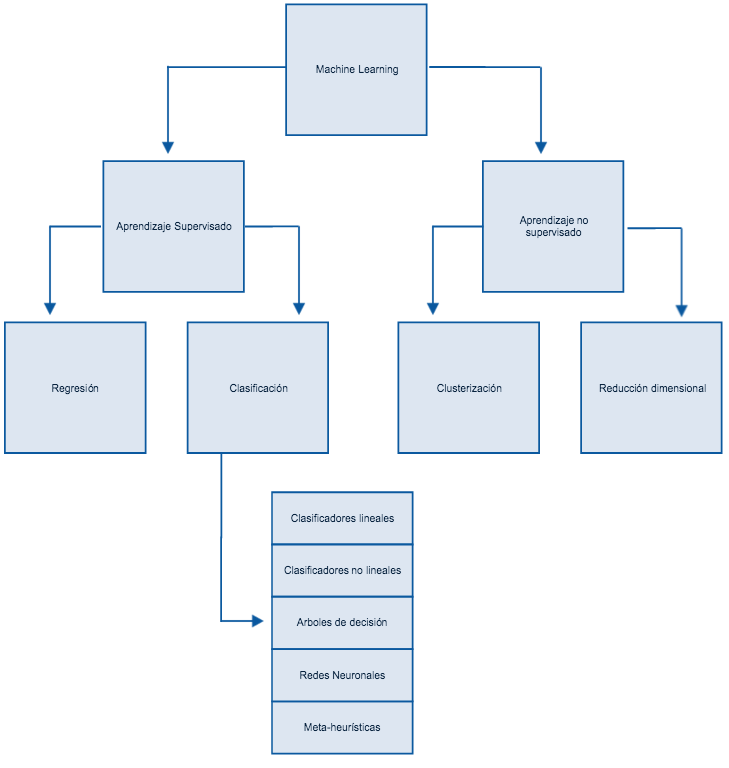
\includegraphics[width=1\textwidth]{Figures/Chapter1_Clasificacion}	
  \caption[Types of learning and the most common methods]
  {Distinct methods to solve problems in Machine Learning}
\end{figure}

\subsection{Fase de inferencia y fase de decisión}

Como primer paso, una vez elegido el método, se selecciona el criterio de penalización de los errores. Este debe ser elegido de manera acorde al problema planteado; por ejemplo, en el caso de una regresión lineal se desea que la penalización sea mayor en los datos que queden muy lejos del ajuste lineal, por lo que se escoge la norma euclidiana \footnote{Además de que las estimaciones hechas a través de mínimos cuadrados bajo ciertos supuestos tienen propiedades deseables de los estimadores: Que sean insesgados y de varianza mínima} $||x||_2 = \sqrt[]{x_{1}^{2}+x_{2}^{2}+ ... + x_{n}^{2}}$. En cambio, en un problema de clasificación se escoge una matriz de penalización o matriz de pérdida, en la que se establece el costo por cada tipo de error de clasificación.

Como segundo paso, se procede con la fase de inferencia, en la que se ajustan los estimadores de los parámetros del modelo elegido de acuerdo a los datos que se tienen, esto con el fin de hacer la inferencia de las distribuciones poblacionales. Como tercer y último paso, se procede a la fase de decisión, en la que se busca encontrar un criterio de decisión que minimice la pérdida esperada \cite{bishop2006pattern}. Por ejemplo, para los problemas de clasificación es muy claro determinar estas dos fases: la primera, se lleva a cabo al determinar la distribución conjunta de clases de pertenencia e individuos; mientras que la segunda, se realiza al determinar las fronteras de decisión basadas en estas probabilidades. Por otra parte, para los problemas de regresión tradicional, ambas fases se realizan al mismo tiempo, ya que al calcular los estimadores de los parámetros se utiliza el método de mínimos cuadrados que minimiza la penalización cuadrática.


\section{Clasificación con modelos lineales}


Se comenzará definiendo la nomenclatura utilizada en esta tesis. Las clases se denotan con la variable aleatoria $k \in C$, con $C  = \{ k = k_j: j = 1, \vdots, K\}$ el conjunto de posibles clases a clasificar y $n(C) = K$ la cardinalidad del conjunto. Para los individuos se define la variable aleatoria $x \in {\rm I\!R}^{m}$. De esta manera, sea $p(x, k)$ \footnote{Teniendo esta probabilidad se pueden calcular fácilmente las probabilidades condicionales $p(k|x)$ y $p(x|k)$} la distribución conjunta de individuos $x$ con clases $k$.


Para la fase de inferencia se utilizan los datos de entrenamiento, donde se distingue a los individuos y a sus clases de pertenencia $x_i \in  {\rm I\!R}^{m}$ y $y_i \in {\rm I\!R}$ respectivamente, con $i = 1, ... , N$. Agrupándolos en matrices, sea $X \in {\rm I\!R}^{N \times m}$ la matriz de individuos y $Y \in {\rm I\!R}^{N \times 1}$ el vector de clases de pertenencia asociada a cada individuo. Una vez hecha la inferencia, se pueden encontrar clases predichas para los individuos $x_i$, se denotará como $\widehat{y_i}$ y $\widehat{Y}$ a la respectiva matriz.


\begin{table}
\caption{Nomenclatura usada en el texto}
\begin{center}
    \begin{tabular}{ | l | c | c | p{4.5cm} |}
    \hline
    Tipo & Definición & Valores & Descripción  \\ \hline
    Entero & $K$ & $K \in \mathbb{N}$ & Número de posibles clases. \\ \hline
    Entero & $N$ & $N \in \mathbb{N}$ & Número de individuos en los datos. \\ \hline
    Entero & $N_k$ & $N_k \in \mathbb{N}$ & Número de individuos en la clase $k$. \\ \hline
    Entero & $m$ & $m \in \mathbb{N}$ & Dimensión de los individuos. \\ \hline
    v.a. & $k$ & $k \in C$ & Variable aleatoria de las clases. \\ \hline
	v.a. & $x$ & $K \in {\rm I\!R}^{m}$ & Variable aleatoria de los individuos. \\ \hline
    Conjunto & $C$ & $k_j: j = 1 ... K$ & Conjunto de posibles clases. \\ \hline
    Dato & $x_i$ & $x_i: i = 1 ... N$ & Vector columna del individuo $i$. \\ \hline
    Dato & $y_i$ & $y_i: i = 1 ... N$ & Dato de clase real del individuo $i$. \\ \hline
    Dato & $\widehat{y_i}$ & $\widehat{y_i}: i = 1 ... N$ & Dato de clase predicha del individuo $i$. \\ \hline
    Dato & $X$ & $X^T = [x_1 |...| x_N]$ & Matriz de individuos. \\ \hline
    Dato & $Y$ & $Y^T = [y_1 | ... | y_n]$ & Vector de clases reales de infividuos. \\ \hline
    Datos & $\widehat{Y}$ & $\widehat{Y}^T = [\widehat{y_1} | ... | \widehat{y_n}]$ & Vector de clases predichas de infividuos. \\ \hline
    Distribución & $p(x,k) $ &  & Distribución conjunta de individuos y clases \\ \hline
    \end{tabular}
\end{center}
\end{table}


\subsection{Fase de inferencia}
Como se mencionaba antes, en fase de inferencia se busca encontrar la distribución conjunta de la muestra con cada una de las clases, es decir $p(x,k)$. La dificultad en estimar esta distribución aumenta conforme la dimensionalidad de $x$ crece y conforme el número de clases aumenta \footnote{Para poder estimar la distribución conjunta, el número de clases debe ser menor que el conjunto de individuos}. Esto es debido a que se comienza a requerir un conjunto de datos mayor para poder estimar cada punto de $p(x,k)$. Por esta razón, muchas veces es suficiente encontrar directamente $p(k|x)$; es decir, dadas las características del individuo, encontrar que tan probable es que pertenezca a cada clase. Por otro lado, en la fase de decisión se encuentra la asignación óptima dependiendo de la matriz de pérdida que se seleccionó y de las probabilidades calculadas (ya sea la distribución conjunta o las condicionales). 

Los modelos propuestos para resolver la fase de inferencia se pueden agrupar de la siguiente manera \cite{bishop2006pattern}: 

\begin{enumerate}
	\item  \textbf{Modelos Probabilísticos Generativos.}
    Plantean resolver el problema de inferencia con el objetivo de determinar $p(x,k)$; es decir, la distribución conjunta de individuos y clases. Una vez obtenida la distribución, se puede usar para calcular $p(x|k)$, $p(k|x)$, $p(x)$ o $p(k)$. Para este enfoque se tienen que hacer supuestos acerca de la distribución de $x$ o $x|k$, o bien, tener un conjunto de entrenamiento muy grande que permita inferir acertadamente $p(x,k)$.

    Tomando propiedades básicas de probabilidad, se pueden calcular las distribuciones necesarias:
  
    \begin{equation} \label{eq:1}
     p(x, k) = p(x|k) p(k)
    \end{equation}

    \begin{equation} \label{eq:2}
     p(x, k) = p(k|x) p(x) 
    \end{equation}
    
    \begin{equation} \label{eq:3}
     p(k|x)  = \frac{p(x|k)p(k)}{p(x)}
    \end{equation}

	\begin{equation} \label{eq:4}
	 p(x) = \sum_{k} p(x|k)p(k) 
	\end{equation}
	
	\begin{equation} \label{eq:5}
	 p(k) = \sum_{x} p(k|x)p(x) 
	\end{equation}
	
	En caso de no tener suficientes datos para inferir directamente esta distribución; o bien, de no tener conocimiento de la estructura de la distribución de $x$, se dan preferencia a los modelos discriminativos o modelos de funciones discriminantes.

\textit{Ventajas\cite{bishop2006pattern}:}
\begin{itemize}
\item Puede ser útil para detectar datos atípicos, ya que al supone una distribución de $x$, se puede determinar qué puntos son poco probables de suceder. De esta manera, se puede encontrar qué predicciones podrían fallar. 
\end{itemize}

\textit{Desventajas\cite{bishop2006pattern}:}
\begin{itemize}
\item Se debe tener información acerca de la distribución de $x$.

\item Inferir directamente de los datos la distribución $p(x,k)$ puede ser muy demandante cuando la dimensionalidad de $x$ es alta. 

\item Si solo se requiere hacer clasificación, puede ser ineficiente encontrar toda la distribución conjunta.
\end{itemize}


\item \textbf{Modelos Probabilísticos Discriminativos.}
Primero, se resuelve el problema de inferencia para determinar $p(k|x)$ con los datos, y después se procede a la fase de decisión para asignar la clase de pertenencia.

\textit{Ventajas:\cite{bishop2006pattern}}
\begin{itemize}
\item Solo se necesita estimar $p(k|x)$ y no toda la distribución conjunta.
\end{itemize}

\textit{Desventajas:\cite{bishop2006pattern}}
\begin{itemize}
\item No se tiene la detección de atípicos presentados por el primer enfoque.
\end{itemize}


\item \textbf{Función Discriminante}
Plantea encontrar una función $\widehat{f}:{\rm I\!R}^m \rightarrow {\rm I\!R}$, tal que clasifique directamente a cada individuo en una clase $k$, de esta manera se define $\widehat{Y}=\widehat{f}(x)$. 

\textit{Ventajas:\cite{bishop2006pattern}}
\begin{itemize}
\item Se combina la fase de inferencia y la fase de decisión en una sola función $\widehat{Y}=\widehat{f}(x)$. 
\end{itemize}

\textit{Desventajas:\cite{bishop2006pattern}}
\begin{itemize}
\item Ya no se cuenta con las probabilidades posteriores $p(k|x)$, por lo que ya no se puede analizar una a una la probabilidad de pertenencia del individuo $x$ a cada una de las clases.
\end{itemize}

\end{enumerate}


\subsection{Fase de decisión}
Para la fase de decisión es conveniente analizar tres definiciones: ``Regiones de decisión'',  ``Fronteras de decisión'' y  ``Funciones discriminantes''. Las primeras dos reciben este nombre porque buscan dividir el espacio al que pertenecen los datos en regiones distintas y excluyentes. Cada una de estas regiones $R_{k}$ clasifica al individuo $x$ en una única clase $k$. En cambio, las fronteras de decisión son las zonas que delimitan una región de las demás; es decir, en ellas (o en sus cercanías) es indiferente qué clase elegir. Por esta razón, es conveniente analizar los datos que quedan cercanos para poder hacer una elección, tomando en cuenta la naturaleza del problema. Por último, las Funciones Discriminantes, nos permiten comparar directamente qué tan verosímil es que un individuo pertenezca a una clase u a otra.

Debido a la finalidad del texto se proponen fronteras lineales \footnote{Las fronteras de decisión pueden tomar formas irregulares, pero en general su forma depende del método de clasificación elegido}, ya que al igual que una regresión lineal, es la base que ejemplifica modelos más complejos. Por este motivo, se mostrarán distintas opciones para construir las regiones y fronteras que se adecuan a los tres enfoques distintos: modelos probabilísticos generativos, modelos probabilísticos discriminativos y funciones discriminantes. 

Para asegurar la linealidad en las fronteras, se debe hacer un análisis que garantice esta propiedad. Se ejemplificará con un caso de dos clases: $k_i$ y $k_j$ con $\left( \begin{array}{ccc}
0 & c_{ij} \\
c_{ji} & 0 \\
 \end{array} \right)$, la matriz de costos con $c_{ij}$ el costo de elegir $i$ cuando la verdadera clase es $j$. Se supone que $c_{ij}, c_{ji}$ mayores que 0. De esta manera la frontera de decisión está dada por:

\begin{equation} \label{eq:6}
c_{ij} p( k = k_i | x \in k_j) - c_{ji} p(k = k_j| x \in k_i) = 0
\end{equation}

De otra manera, si $c_{ij} p( k = k_i | x \in k_j) < c_{ji} p( k = k_j| x \in k_i) $ o viceversa, entonces se clasificará hacia $k_i$ y $k_j$, respectivamente. Para los fines de esta tesis, se tomarán los costos de $c_{ij} = c_{ji} = 1$ ya que esto solo juega en la ordenada al origen de la ecuación de la frontera lineal. Tomando un resultado presentado por T. Mitchell \cite{mitchell2006discipline}, si se aplica una función monótona de $p(k, x)$, la linealidad de las fronteras de decisión se mantiene. En este caso, se toma la función de logaritmo $log()$:


$$ log(p(k = k_j | x)) = log( p(k = k_i | x)) $$	

\begin{equation} \label{eq:7}
 log \frac{p( k = k_j | x )}{ p(k =  k_i |  x)} = 0 	
\end{equation}

El lado izquierdo de esta última ecuación es conocido como razón de momios (log odd). Cuando es una función lineal con respecto a $x$, mantiene la linealidad de la frontera:

\begin{equation} \label{eq:8}
 log \frac{p(k = k_j | x )}{p(k = k_i |  x)} = \beta_0 + x^T \beta_1 
\end{equation}


\section{Métodos de clasificación lineales}

En la fase de inferencia se busca construir la distribución $p(x,k)$, la cual será usada en la fase de decisión para tomar un criterio óptimo de clasificación. En la sección 2.2 se mostraron los distintos enfoques que se toman para hacer esta inferencia. Recapitulando, para modelos generativos se escoge $\widehat{Y}(x) = \widehat{f}(p(x,k))$; para modelos discriminativos $\widehat{Y}(x) = \widehat{f}(p(k|x))$ y para funciones discriminantes se escoge $\widehat{Y}(x)$ = $\widehat{f}(x)$. En los dos primeros casos se ve que la función $f$ toma como entrada distribuciones concernientes a $x$ y $k$, pero en el tercer caso, solamente toma como entrada a $x$. En esta sección se ejemplificarán los 3 métodos con técnicas sencillas. Para el enfoque Probabilístico Generativo se empleará el Análisis Discriminante Lineal, para el Probabilístico Discriminativo la Regresión Logística y para la función discriminante, el Discriminante Lineal de Fisher.

En los siguientes tres ejemplos se explica cómo se realiza la inferencia de las distribuciones, para después demostrar la linealidad en las fronteras. Como se explica en la sección 2.2.2, si se asegura que (\ref{eq:8}) es lineal con respecto a $x$, entonces se garantiza la linealidad de estas. En la Regresión Logística se ejemplificará el procedimiento para $n$ clases. Para los demás se supondrá el caso de la frontera entre dos clases.


\subsection{Modelos discriminativos: Regresión Logística}


\textit{Inferencia de la distribución $p(k | x)$} \\
Para la fase de inferencia, se calculan las probabilidades posteriores de pertenecer a cada grupo $j$, de manera que: 
\begin{equation} \label{eq:15}
	\sum\limits_{j = 1}^{K} p(k = k_j | x) = 1
\end{equation}


\textit{Linealidad de la frontera}\\
Para obtener la estimación de las $K$ distribuciones de probabilidad $p(k = k_j | x)$, se parte de la ecuación (\ref{eq:8}) y se supone que todas las fronteras son lineales.

$$ \log \frac{p(k = k_1 | x)}{p(k = k_K | x)} = \beta_{1.0} + \beta_1^T x$$

$$ \log \frac{p(k = k_2 | x)}{p(k = k_K | x)} = \beta_{2.0} + \beta_2^T x$$

$$\vdots$$

$$ \log \frac{p(k = K-1 | x)}{p(k = k_K | x)} = \beta_{(K-1).0} + \beta_{(K-1)}^T x$$

Con estas ecuaciones se crea un sistema que cuenta con $K$ variables $p(k = k_j| x)$ y $K-1$ ecuaciones, lo cual, añadiendo la restricción (\ref{eq:15}) se puede despejar cada probabilidad: 

$$ p(k = k_1 | X = x) = \frac{\exp(\beta_{1.0} + \beta_1^T x)}{1+\sum\limits_{i=1}^{K-1} {\exp(\beta_{l.0} + \beta_l^T x)}} $$

$$ p(k = k_2 | X = x) = \frac{\exp(\beta_{2.0} + \beta_2^T x)}{1+\sum\limits_{i=1}^{K-1} {\exp(\beta_{l.0} + \beta_l^T x)}} $$

$$ \vdots $$

$$ p(k = k_{K-1} | X = x) = \frac{\exp(\beta_{(K-1).0} + \beta_{(K-1)}^T x)}{1+\sum\limits_{i=1}^{K-1} {\exp(\beta_{l.0} + \beta_l^T x)}} $$

Para la clase de referencia: 

$$ p(Y = k_K | X = x) = \frac{1}{1+\sum\limits_{i=1}^{K-1} {\exp(\beta_{l.0} + \beta_l^T x)}} $$

Para tener la formulación completa, falta estimar las $\beta$ de cada probabilidad. Esto, comúnmente, se realiza con máxima verosimilitud (a través de métodos iterativos como Newton) \cite{hastie2009elements}


\textit{Funciones $logit$ y $logit^{-1}$} \\
Para este modelo es conveniente analizar la función logit y su inversa:
 
 \begin{equation} \label{eq:16}
 logit = \log (\frac{p}{1-p}) 
 \end{equation}

\begin{equation} \label{eq:17}
 logit^{-1}  = \frac{\exp(x)}{1+\exp(x)}
 \end{equation}


Al graficar la función $logit$ y la $logit^{-1}$ sobre un plano (Figura 1.1) se observan algunas de sus propiedades. En la gráfica de la izquierda, se realiza un mapeo de valores del rango (0,1) al rango (-$\inf$,$\inf$), mientras que a la derecha se transforman valores continuos de (-$\inf$, $\inf$) al $(0,1)$. La transformación realizada por $logit^{-1}$ es de mayor interés ya que su rango es semejante al que toman las probabilidades. Este enfoque nos da una amplia gama de elección para la fase de decisión, ya que deja elegir los puntos de corte para cada clase, dependiendo la penalización que se quiera dar a cada tipo de error \cite{hastie2009elements}:

\begin{figure}[!ht]
  \centering
	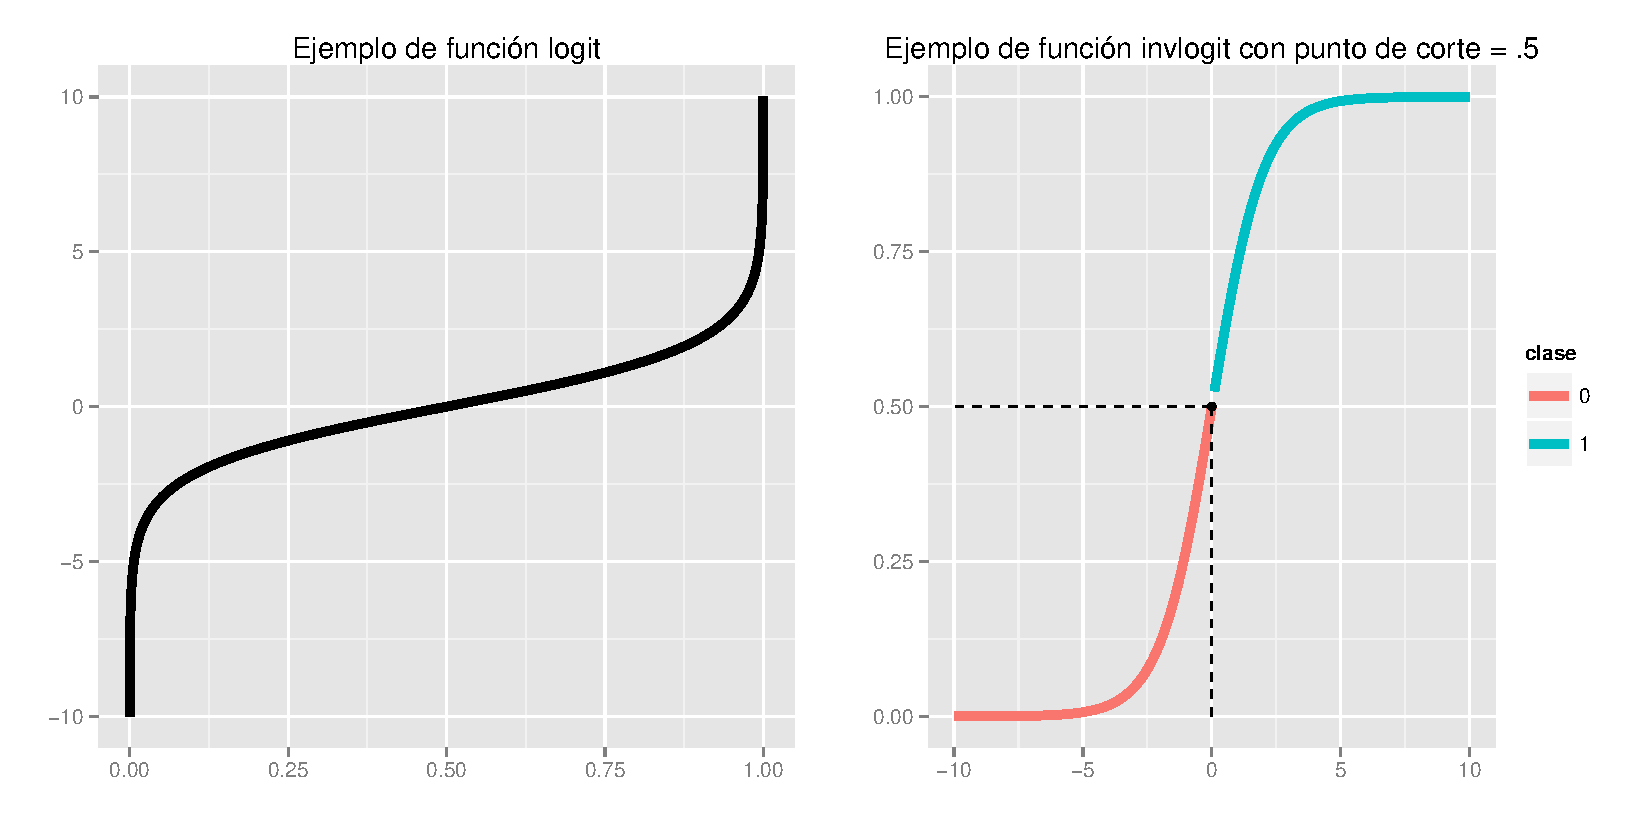
\includegraphics[width=1\textwidth]{Figures/Chapter1_logit}	
  \caption[Función logit y $logit^{-1}$]
  {En la izquierda se muestra la función logit y en la derecha la función $logit^{-1}$ con punto de corte p = .5; es decir, se escoge la clase 1 en la zona azul y la clase 0 en la zona roja.}
\end{figure}

\pagebreak
\subsection{Modelos generativos: Análisis Discriminante Lineal}


\textit{Inferencia de la distribución $p(x,k)$}\\
Para el caso del Análisis Discriminante Lineal se sigue un enfoque generativo, en el que se realiza inferencia de $p(x,k)$. Primero, se supondrá que $p(x|k)$ sigue una distribución Gaussiana con varianza $\Sigma_{k}$ constante para todas las clases y $\mu_{k}$ la media de los individuos pertenecientes a la clase $k$ (ecuación (\ref{eq:9})). Por otra parte, se estima la distribución $p(k)$ como la proporción de casos que cada clase aparece en los datos (ecuación (\ref{eq:10})). Usando la ecuación (\ref{eq:1}) se deduce $p(x,k)$:


\begin{equation} \label{eq:9}
 p(x|k) = \frac{1}{(2\pi) |\Sigma|^{1/2}} e^{-\frac{1}{2}(x-\mu_{k})^{T}\Sigma^{-1}(x-\mu_{k})}
\end{equation}

\begin{equation} \label{eq:10}
 p(k) = \frac{N_k}{N}	
\end{equation}

Por otro lado, al utilizar el Teorema de Bayes (\ref{eq:3}) y la ecuación (\ref{eq:4}), se puede calcular $p(k|x)$ directamente. 



\textit{Linealidad de la frontera}\\
Al hablar de la linealidad de la frontera, se tiene que cumplir la ecuación (\ref{eq:8}), enunciada en la sección 2.2.2:

$$\log \frac{p(k = k_j | x )}{p(k = k_i |  x)} = \beta_0 +  x^T \beta_1$$

$$\log \frac{p(x | k = k_j)p(k = k_j)}{p( x | k = k_i)p(k = k_i)} = \beta_0 +  x^T \beta_1$$

\begin{equation} \label{eq:11}
 	\log\frac{p(x | k = k_j)}{p(x | k = k_i)} + \log\frac{p(k = k_j)}{p(k = k_i)} = \beta_0 +  x^T \beta_1
\end{equation} 

La ecuación (\ref{eq:11}) consta de dos sumandos. Al desarrollar el primero:

$$ \log\frac{p(x | k = k_j)}{p(x | k = k_i)} = -\frac{1}{2}[(x - \mu_j)^T \Sigma^{-1}(x - \mu_j) - (x - \mu_i)^T \Sigma^{-1}(x - \mu_i)] $$ 


\begin{equation}
\begin{aligned}
 \log\frac{p(x | k = k_j)}{p(x | k = k_i)} =& -\frac{1}{2}[{\mu_j}^T \Sigma^{-1} {\mu_j}  -  {\mu_i}^T \Sigma^{-1} {\mu_i}]  + \\
 &\frac{1}{2}[{x}^T \Sigma^{-1}(\mu_j-\mu_i) - {(\mu_j-\mu_i)}^T \Sigma^{-1}(x)
\end{aligned}
\end{equation}

 

 \begin{equation} \label{eq:12}
 	\log\frac{p(x| k = k_j)}{p(x | k = k_i)} = -\frac{1}{2}[{(\mu_j - \mu_i)}^T \Sigma^{-1} {(\mu_j + \mu_i)}] + [{x}^T \Sigma^{-1}(\mu_j-\mu_i)]
 \end{equation}

Sustituyendo \ref{eq:12} en \ref{eq:11} se tiene como resultado:

$$ \log \frac{p(k = k_j)}{p(k = k_i)} - \frac{1}{2}[(\mu_j - \mu_i)^T \Sigma^{-1} (\mu_j + \mu_i)] + {x}^T \Sigma^{-1} (\mu_j - \mu_i) = \beta_0 +  x^T \beta_1$$

Del cual se nota que $\beta_0$ y $\beta_1$ son equivalentes a:

\begin{equation} \label{eq:13}
\beta_0 = \log \frac{p(k = k_j)}{p(k = k_i)} - \frac{1}{2}[(\mu_j - \mu_i)^T \Sigma^{-1} (\mu_j +\mu_i)] 	
\end{equation}

\begin{equation} \label{eq:14}
 \beta_1 = \Sigma^{-1} (\mu_j -\mu_i)
\end{equation}


\textit{Funciones Discriminantes} \\
Ahora, solo falta enunciar las funciones discriminantes de la clase $i$ y $j$; es decir, $log p(k = k_i | x)$ y  $log p(k = k_j | x)$, respectivamente:
$$ \delta_j (x) = \log {p(k = k_j)} - \frac{1}{2}\mu_j^T \Sigma \mu_j + x^T \Sigma^{-1} \mu_j$$
$$ \delta_i (x) = \log {p(k= k_i)} - \frac{1}{2}\mu_i^T \Sigma \mu_i + x^T \Sigma^{-1} \mu_i$$


\subsection{Funciones Discriminantes: Discriminante Lineal de Fisher}

El Discriminante Lineal de Fisher es similar al Análisis Discriminante Lineal. El primero permite ver una proyección informativa en un espacio de dimensión menor \cite{hastie2009elements}. Este planteamiento fue propuesto por Fisher \cite{fisher1936use}, y hace referencia a un discriminante lineal con menos supuestos \footnote{No toma en cuenta la distribución de los datos, ni la igualdad de varianzas entre las clases.}. Propone los supuestos de definir una varianza entre clases que es la varianza de las medias de las clases, y una varianza intra-clase, que mide la varianza dentro de las clases con respecto a la media de cada clase. Después, se busca una matriz de proyección $V$ que maximice la dispersión entre-clase al mismo tiempo que minimiza la dispersión intra-clase \cite{ngo2012trace}.

Se comenzará definiendo la nomenclatura necesaria para la sección. Sea $N_{k}$ el número de personas en la clase $k$, $N$ el número total de personas y $w_i = V^T x_i$; es decir, los datos proyectados con la matriz $V$. Entonces, se definen las medias de grupo $k$ como $\mu_k$ y la media de todos los datos $x_i$ como $\mu$:

\begin{equation} \label{eq:18}
 	\mu_k = \frac{1}{N_{k}} 
 	\sum_{\substack{i = 1\\
                  	y_i = k}}^{N}
                  x_i
\end{equation} 


\begin{equation} \label{eq:19}
 \mu = \frac{1}{N} \sum_{i = 1}^{N} x_i
\end{equation}

Por otro lado, se definen las medias correspondientes a los datos proyectados $w_i$:
\begin{equation} \label{eq:20}
 	\widetilde{\mu_k} = \frac{1}{N_{k}} 
 	\sum_{\substack{i = 1\\
                  	y_i = k}}^{N}
                  w_i
\end{equation} 


\begin{equation} \label{eq:21}
 \widetilde{\mu} = \frac{1}{N} \sum_{i = 1}^{N} w_i
\end{equation}


La matriz de dispersión intra-clase de los datos proyectados:


$$\Phi_{I} = \sum_{k=1}^{K} 
				\sum_{\substack{i = 1\\
                  			   	y_i = k}}
                    ^{N}
           ||w_i-\widetilde{\mu}_{k}||^{2}_{2}$$


$$ \Phi_{I} =  \sum_{k=1}^{K} 
					\sum_{\substack{i = 1\\
                  			   	y_i = k}}
                    ^{N}
			Tr (V^T (x_i - \mu_k)(x_i - \mu_k)^T V ) $$

\begin{equation} \label{eq:22}
 \Phi_{I} =  Tr(V^T S_I V) 
\end{equation}



\begin{equation} \label{eq:23}
con \quad S_I = \sum_{k=1}^{K} 
					\sum_{\substack{i = 1\\
                  			   	y_i = k}}
                    ^{N}
 ({x_i-\mu_{k}})({x_i-\mu_{k}})^T 
\end{equation}



La matriz de dispersión entre-clases de los datos proyectados:

$$ \Phi_{E} = \sum_{k=1}^{K} N_{k} || \widetilde{\mu}_k - \widetilde{\mu} ||^{2}_{2} $$

$$ \Phi_{E} = \sum_{k=1}^{K} N_{k} || V^T \mu_k - V^T \mu ||^{2}_{2} $$
 
$$ \Phi_{E} =  \sum_{k=1}^{K} N_{k} V^T(\mu_k - \mu)(\mu_k - \mu)^T V $$
\begin{equation} \label{eq:24}
 \Phi_{E} =  Tr(V^T S_E V)  
\end{equation}

\begin{equation} \label{eq:25}
 con \quad S_E = \sum_{k=1}^{K} N_{k} (\mu_k - \mu)(\mu_k - \mu)^T 
\end{equation}

De este modo, se definen las dos matrices importantes del método: $S_I$ la matriz de dispersión interna y $S_E$ la matriz de dispersión entre clases. Con estas definiciones surge la idea intuitiva de maximizar $\Phi_{E}$ al mismo tiempo que se minimiza $\Phi_{I}$; es decir, encontrar un espacio de proyección en el que los grupos pertenecientes a la misma clase tengan poca varianza, al mismo tiempo que la varianza entre estas clases sea alta. Se puede plantear esta idea a través del problema de maximización:

\begin{equation}\label{eq:26}
	\max_{\substack{V \in {\rm I\!R}^{n\times p} \\ V^TV = I}} \frac{Tr(V^T S_E V)}{Tr(V^T S_I V)} 
\end{equation}

Este problema de optimización es el principal tema de la tesis, por lo que los detalles acerca de las fronteras y el proceso de maximización que derivan en encontrar la matriz óptima $V$ será analizado en los capítulos siguientes.

\section{Enfoques para la minimización del error}

La teoría de la decisión se aplica para la fase dos, en la que se busca tomar decisiones óptimas dadas las probabilidades calculadas en la fase de inferencia. La motivación de una teoría de la decisión es que las probabilidades, por sí solas, no nos indican que clase elegir, solamente nos dan información del comportamiento de la distribución. Por esta razón, es conveniente saber que decisión tomar basándonos en la penalización de los errores elegidos anteriormente. Puede verse desde dos perspectivas \footnote{En realidad el primer enfoque es un caso particular del segundo}:

\begin{itemize}
\item Minimizar el error de clasificación a lo largo de todos nuestros datos.
\item Minimizar la pérdida esperada dada una matriz de pérdida L. 
\end{itemize}


\subsection{Minimizando el error de clasificación}
Esta regla dividirá el espacio en regiones $R_j$ en las que cada individuo es asignado a una clase $k_j$ con $j = 1, ... , K$. Recordando la nomenclatura, $x_i$ es el individuo $i$ y $y_i$ es la clase a la que pertenece este sujeto; mientras que $\widehat{y}_i$ es la clase predicha del sujeto $i$. Por otro lado, $k_j$ es la clase $j$ de las $K$ existentes. Para encontrar la decisión óptima de elección se busca minimizar la probabilidad de cometer errores, que está dada por:

%$$p(error) = 1 - \sum_{i = 1}^{N} \sum_{j=1}^{K} p(y_i = k_j, \widehat{y}_i = k_j)$$


$$p(error) = 1 - \sum_{i = 1}^{N} \sum_{j=1}^{K} p(x_i \in R_{j}, y_i = k_j)$$

En la expresión anterior, cuando $x_i \in R_j$ se sabe que $\widehat{y}_i$ esta asociada a la clase $k_j$. Ocupando la igualdad $p(x \in R_{j}) = \int_{R_j} p(x) dx$ se tiene que es equivalente a maximizar la probabilidad de no cometer errores:

$$p(no error) = \sum_{i = 1}^{N} \sum_{j=1}^{K} p(x_i \in R_{j},  y_i = k_j)$$

$$p(no error) = \sum_{i = 1}^{N} \sum_{j=1}^{K} \int_{R_j} p(x_i, y_i = k_j) dx $$

Es facil deducir que $\int_{R_j} p(x_i, y_i = k_j) dx$ es equivalente a que $p(\widehat{y}_i = k_j, y_i = k_j)$ porque cuando $x_i$ está en la región $R_j$, entonces $\widehat{y}_i = k_j$. Ocupando esta igualdad se puede deducir:

\begin{equation}\label{eq:27}
p(no error) = \sum_{i = 1}^{N} \sum_{j=1}^{K} p(\widehat{y}_i = k_j, y_i = k_j) 
\end{equation}

Es decir, dado que $x_i$ pertenece a la región $R_{j}$ (y por lo tanto es clasificado en la clase $k_j$) y la clase original de $x_i$ es $y = k_j$, implica que la clasificación es correcta. La maximización de (\ref{eq:27}) sigue un argumento intuitivo. Al obtener la distribución $p(x, k)$, se selecciona aquella que tiene la probabilidad más alta de ocurrir para cada individuo; es decir, tomar como criterio de decisión la que tenga mayor $p(x_i \in R_j)$. 

En los Modelos Probabilísticos Generativos se utiliza la distribución conjunta, en cambio en los discriminativos solamente se utiliza $p(k|x)$. Para extender el resultado anterior a la distribución condicional se ocupa la ecuación $\ref{eq:2}$:

$$p(x,k)  = p(k|x)p(x)$$

Maximizar $p(x,k)$ es equivalente a maximizar el término de la derecha. Como $p(x)$ es positivo y común a todos los términos, es equivalente a seleccionar la clase con probabilidad $p(k|x)$ más grande para cada individuo. 

\subsection{Minimizando la pérdida esperada}

Tomando una matriz de pérdida se puede ver más general el error de clasificación. La motivación de este enfoque es la disparidad en los distintos costos asociados a cada tipo de error de clasificación. Por ejemplo, en un problema en el que se predice si a un paciente le dará un ataque al corazón, es peor predecir que no tendrá un ataque cuando en realidad si lo tendrá \cite{hastie2009elements}. Por esta razón, la modelación del error a través de una matriz de pérdida tiene sentido. Sea $L$ la matriz que tiene como característica el tener ceros en la diagonal y pesos no negativos en cualquier otro lado y $L(X,Y)$ el costo asociado a elegir Y cuando la clase verdadera es X. \footnote{Es fácil notar que la matriz $L_{0-1}$; es decir, 0 sobre la diagonal (Clasificación correcta) y 1 (Clasificación incorrecta) en cualquier otro lugar, es equivalente al enfoque que minimiza el error de clasificación}

Tomando el error esperado de predicción de los vectores $Y$ y $\widehat{Y}$ bajo la matriz $L$:

$$ EEP = E[L(Y, \widehat{Y})] $$

En la que $Y$ es el vector de clases de pertenencia verdaderas y $\widehat{Y}$ es el vector de clases de pertenencias predichas. Ambos vectores son de variables categóricas que pueden tomar valores $k_j \in C$ con $j = 1 ... K$. 

Al desarrollar el error esperado de predicción como una sumatoria sobre los $N$ individuos y las $K$ clases, es equivalente a:

$$EEP = \sum_{i = 1}^{N} \sum_{j=1}^{K} L[y_i = k_j, \widehat{y}_i = k_j] p(x = x_i, k = k_j)$$

Sustituyendo $p(k, x) = p(k | x)p(x)$, se puede calcular la esperanza sobre los individuos $x$. Lo que se deduce la expresión:

$$EEP = E_{x} \sum_{j=1}^{K} L[y = k_j, \widehat{y} = k_j] p(k_j | x)$$

Como se busca minimizar el error esperado de predicción con respecto a $\widehat{y}$, se obtiene el siguiente problema de minimización:

$$\widehat{y}^{*} = \argmin_{\widehat{y}} E_{x} \sum_{j=1}^{K} L[y = k_j, \widehat{y} = k_j] p(k_j | x)$$

Este problema de minimización es equivalente a minimizar el error esperado de predicción para cada individuo $x$:

$$\widehat{y}^{*} = \argmin_{\widehat{y}} \sum_{j=1}^K L[y = k_j, \widehat{y} = k_j]p(k_j|x)$$

Al escoger la función de pérdida $0-1$, cuando $\widehat{y}^{*} = y$, entonces la pérdida es igual a 0, por lo que la fórmula se simplifica a:

$$\widehat{y}^{*} = \argmin_{\widehat{y}}
\sum_{\substack{j = 1 \\
			   y \neq \widehat{y}}} ^ K 
			   L[y = k_j, \widehat{y} = k_j] p(k_j | x)$$

Por otro lado, cuando $\widehat{y}^{*} \neq y$ entonces la pérdida es igual a 1:

$$\widehat{y}^{*} = \argmin_{\widehat{y}}
\sum_{\substack{j=1 \\
      y \neq \widehat{y}}}^K
p(k_j | x)$$

$$\widehat{y}^{*} = \argmin_{\widehat{y}} 
[1 - \sum_{\substack{j=1 \\
      y = \widehat{y}}}^K
p(k_j|x)]$$

Esta expresión es equivalente a maximizar:

$$\widehat{y}^{*} = \argmax_{\widehat{y}} p(k|x)$$

De esta manera, se escoge $\widehat{y}^{*}$ como la probabilidad posterior más grande de pertenencia a la clase $k$ dado $x$. Esta solución es conocida como ``Clasificador de Bayes'' y nos dice que hay que clasificar a las clases más probables usando la distribución condicional $p(k|x)$. La tasa de error de este clasificador se le conoce como ``Tasa de Bayes''\cite{hastie2009elements}.



 
	\chapter{Discriminante Lineal de Fisher}
\label{ch:chapter2}

En este capítulo se hablará del Análisis Discriminante Lineal de Fisher (ADLF), el cual busca optimizar un cociente de la forma $Tr(V^T A V) / Tr(V^T B V)$ sobre el conjunto de matrices ortogonales $V$ con $A, B$ matrices positivas definidas. Para resolver el ADLF, se han presentado en libros de aprendizaje estadístico y clasificación de patrones formulaciones alternas al problema original, ya que este era considerado computacionalmente muy costoso \cite{wang2007trace}\cite{ngo2012trace}. Planteamientos como: maximizar la traza de la matriz de dispersión entre clases sujeto a una restricción sobre la matriz de dispersión interna, maximizar la traza del cociente de matrices; o bien, maximizar el cociente de determinantes, han sido formulaciones presentadas en distintos textos \cite{duda2012pattern} \cite{hastie2009elements} \cite{mitchell2006discipline} \cite{fukunaga2013introduction}. Al final, todas estas propuestas resultan ser versiones simplificadas del problema.

En este capítulo se resolverá el problema original del ADLF a través del método de Newton-Lanczos, el cual resulta ser computacionalmente eficiente. En la primer sección del capítulo se contextualizará al problema dentro del área de Aprendizaje de Máquina. En la segunda parte, se proporcionará la teoría correspondiente para seguir con facilidad el texto. Por último, en la tercera parte, se plantea la solución al problema de ADLF para una dimensión, se generaliza a $p$ dimensiones y se proporcionan las condiciones para la existencia de la solución.


\section{Aprendizaje de máquina}
El Aprendizaje de Máquina toma como base dos áreas de investigación: la Ciencia de la Computación y la Estadística. De la primera, retoma las preguntas: ¿Cómo se pueden construir máquinas que resuelvan problemas? Y ¿Qué problemas son tratables o intratables? De la segunda, toma las preguntas: ¿Qué puede ser inferido de los datos? ¿Bajo que supuestos del modelo? Y ¿Con qué confiabilidad? \cite{mitchell2006discipline}. El esfuerzo por resolver estas preguntas da como resultado una disciplina enfocada a construir teorías estadístico-computacional de los procesos de aprendizaje.

\subsection{Procesos de aprendizaje}

Se dice que una máquina ``aprende" dada una tarea (T), una medición del rendimiento (R) y un tipo de experiencia (E) si el sistema mejora confiablemente su rendimiento (R) en la tarea (T) dada la experiencia (E) \cite{mitchell2006discipline}. Es decir, se modela una estructura con los datos proporcionados de manera que el rendimiento en la tarea mejora conforme más información recibe. La diversidad de las tareas, así como el campo de aplicaciones es muy diverso, por ejemplo:

\begin{itemize} 

\item \textit{Clasificación de spam/no-spam}, en el que (E) son los correos, (T) el clasificar correctamente el \textit{spam} y (R) el porcentaje de correos correctamente clasificados.

\item \textit{Reconocimiento/Clasificación facial}, en el que (E) son los rostros de distintas personas, (T) el reconocimiento o clasificación de los rostros y (R) el porcentaje de rostros correctamente reconocidos o clasificados.
\end{itemize} 

Los procesos de aprendizaje tienen diversas aplicaciones y distintos supuestos, por lo que han surgido clasificaciones para analizarlos en conjunto. La utilizada en este texto es la propuesta por T. Hastie \cite{hastie2009elements}, la cual divide a los métodos en dos grupos: aprendizaje supervisado y aprendizaje no supervisado. El primero, supone la presencia de una variable de salida que actúa como guía en la construcción de la estructura. Ejemplos de éste es la regresión lineal, los árboles de decisión y las máquinas de soporte vectorial. 
Por otra parte, el aprendizaje no supervisado solo cuenta con la información de las variables independientes; por ejemplo, análisis de conglomerados, reglas de asociación y reducción dimensional. 

Después de esta primer clasificación, se subclasifica a los métodos de aprendizaje supervisado de acuerdo al tipo de variable de salida (Figura 1.1). \footnote{A lo largo del texto se usará indiferentemente variable de entrada como ``input'' o variable independiente y variable de salida como ``output'' o variable dependiente} Cuando se trata de una variable cuantitativa recibe el nombre de regresión, mientras que en el caso de cualitativas se le llama clasificación. Por otra parte, el aprendizaje no supervisado tiene dos ramas en las que el texto hace énfasis \cite{hastie2009elements}: Segmentación en el caso que se desee asignar un grupo a cada individuo, de manera que los grupos sean homogéneos entre sí; o bien, reducción dimensional cuando solamente se desea proyectar a los individuos en un espacio de menor dimensión, de manera que se cumplan características especiales en dicho subespacio. 

El problema de ADLF pertenece a la rama de aprendizaje supervisado, en particular a los métodos clasificación. Alternativas para esta finalidad, y que sigan asumiento linealidad en la frontera, son la Regresión Logística, el Análisis Discriminante Lineal y las Máquinas de Soporte Vectorial. 

\begin{figure}[!ht]
  \centering
  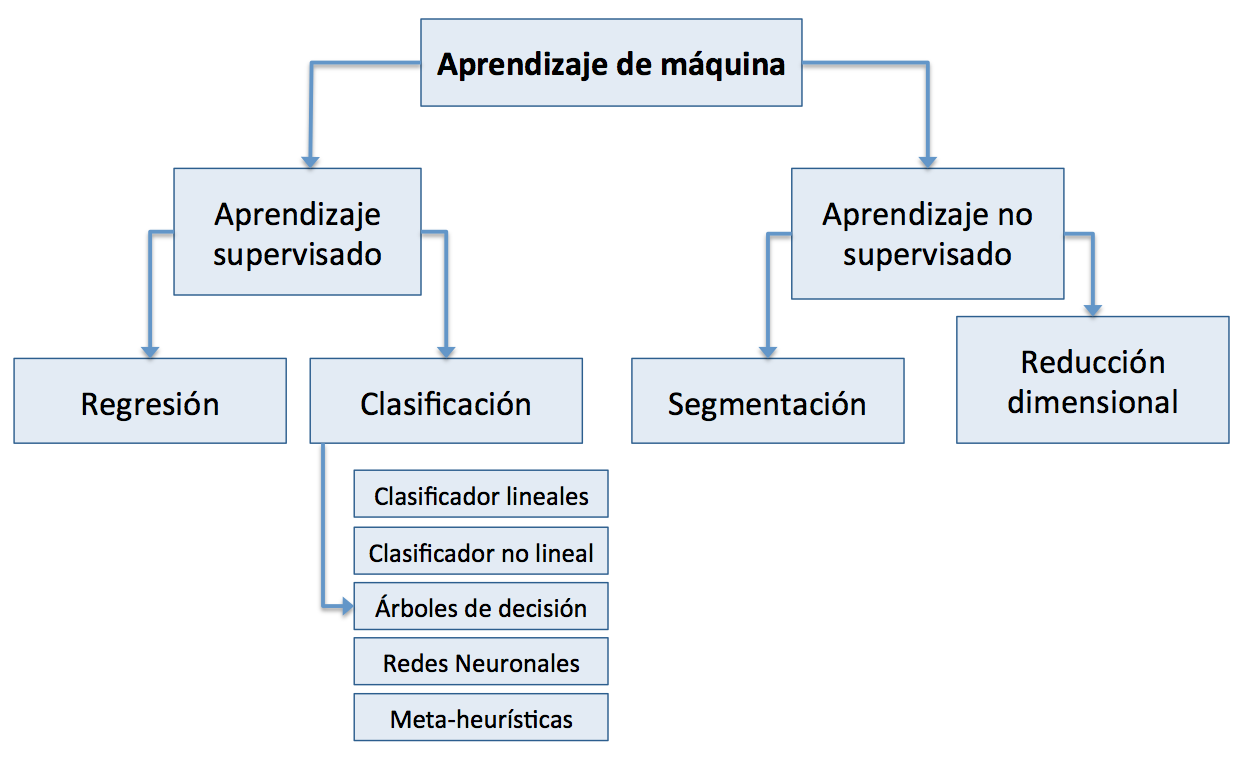
\includegraphics[width=1\textwidth]{Figures/Chapter1_Clasificacion1.png} 
  \caption[Enfoques para resolver problemas de clasificación.]
  {Distintos enfoques para resolver problemas de clasificación en el área de Aprendizaje de Máquina.}
\end{figure}

\section{Matrices de dispersión}
Se comenzará definiendo la nomenclatura necesaria para la sección. Sea $x_i$ el individuo $i$ que pertenece a la clase $y_i$, $N_{k}$ el número de personas en la clase $k$, $N$ el número total de personas y $w_i = V^T x_i$; es decir, los datos proyectados con la matriz $V$. Entonces, se definen las medias de grupo $k$ como $\mu_k$ y la media de todos los datos $x_i$ como $\mu$:

\begin{equation} \label{eq:18}
  \mu_k = \frac{1}{N_{k}} 
  \sum_{\substack{i = 1\\
                    y_i = k}}^{N}
                  x_i
\end{equation} 

\begin{equation} \label{eq:19}
 \mu = \frac{1}{N} \sum_{i = 1}^{N} x_i
\end{equation}

Por otro lado, se definen las medias correspondientes a los datos proyectados $w_i$:
\begin{equation} \label{eq:20}
  \widetilde{\mu_k} = \frac{1}{N_{k}} 
  \sum_{\substack{i = 1\\
                    y_i = k}}^{N}
                  w_i
\end{equation} 

\begin{equation} \label{eq:21}
 \widetilde{\mu} = \frac{1}{N} \sum_{i = 1}^{N} w_i
\end{equation}

El ADLF hace amplio uso de las matrices de dispersión, en específico de la matriz de covarianza, la matriz de dispersión de todos los individuos, la matriz de dispersión interna y la matriz de dispersión entre clases. Es importante analizar a profundidad la terminología y las fórmulas que se usarán a lo largo de la tesis para entender la lógica detrás de la formulación.

Sea $\Sigma$ la matriz de covarianza (\textit{Covariance Matrix)} de todos los individuos. Se define como $\widehat{\Sigma}$ al estimador insesgado de $\Sigma$ el cual está escalada entre $N-1$:

\begin{equation} \label{eq:2.1}
\widehat{\Sigma} = \frac{1}{N-1} \sum_{i=1}^{N}(x_i - \mu)(x_i - \mu)^T	
\end{equation}

Si esta matriz no está escalada por $N-1$ entonces se le conoce como matriz de dispersión (\textit{Scatter Matrix}), en esta tesis se representará como $S_T$, con el subíndice $T$ que significa que está tomando en cuenta a todos los individuos:

\begin{equation} \label{eq:2.2}
S_T = \sum_{i=1}^{N}(x_i - \mu)(x_i - \mu)^T	
\end{equation}

Cuando solo se toman a los individuos de una clase particular $k$, se puede encontrar su correspondiente matriz de dispersión, representada como $S_k$, con el subíndice $k$ simbolizando que está tomando en cuenta solo a los individuos de la clase $k$:

\begin{equation*}
S_k = \sum_{\substack{i=1 \\ y_i = k}}^{N} (x_k - \mu)(x_k - \mu)^T	
\end{equation*}

De esta manera se define la matriz de dispersión interna (\textit{Within-class scatter matrix}) como la suma sobre $k$ de todas las matrices de dispersión de cada clase:

\begin{equation}\label{eq:2.3}
S_I = \sum_{k=1}^{K} 
					\sum_{\substack{i = 1\\
                  			   	y_i = k}}
                    ^{N}
 ({x_i-\mu_{k}})({x_i-\mu_{k}})^T 	
\end{equation}

Ahora solo falta definir la matriz de dispersión entre clases (\textit{Between-class scatter matrix}) como la suma de diferencias al cuadrado de las medias de clase contra la media de todos los datos multiplicada por el número de individuos en cada clase $N_k$:

\begin{equation} \label{eq:2.4}
S_E = \sum_{k = 1}^K N_k (\mu_k - \mu)(\mu_k - \mu)^T	
\end{equation}

\begin{figure}[!ht] \label{Fig1.1}
  \centering
	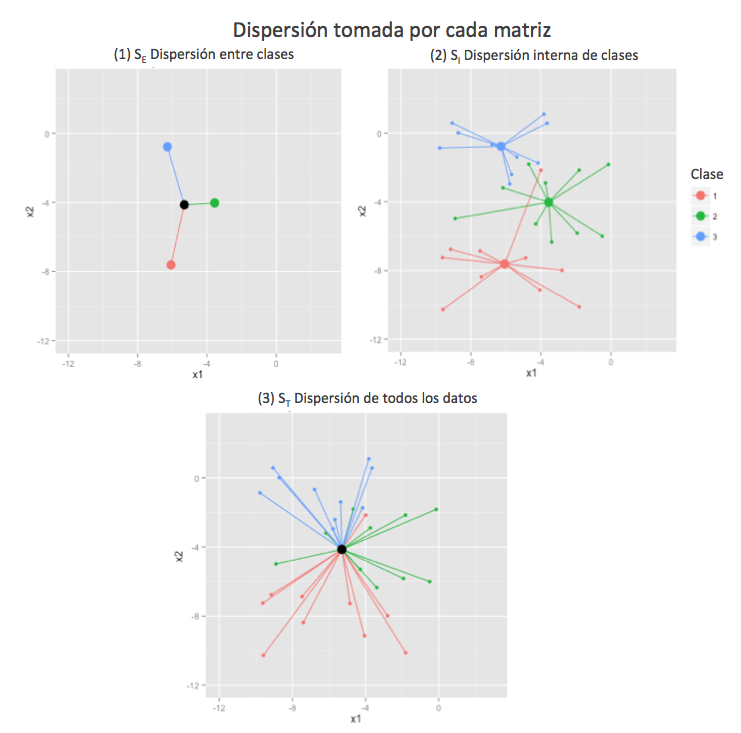
\includegraphics[width=1\textwidth]{Figures/Chapter2_SE_SI}	
  \caption[Distancias en las matrices de dispersión.]
  {En la gráfica (1) se representa la $S_E$, es decir las distancias al cuadrado entre la media de todos los datos (Punto negro) y las medias de cada clase (Puntos de color gruesos). La gráfica (2) representa $S_I$; es decir, la distancia al cuadrado de los individuos a la media de su clase. La gráfica (3) representa $S_T$, la dispersión de los datos con respecto a la media de todos.}
\end{figure}

Entre la matriz de dispersión interna $S_I$, la matriz de dispersión entre clases $S_E$ y la matriz de dispersión total $S_T$ existe una relación importante. Se cumple que $S_T = S_I + S_E $; es decir, la dispersión de las medias de grupos con la media global más la dispersión de cada clase individual es igual a la dispersión de los datos sin la información de las clases. Los datos de la figura 1.2 representan las distancias que toman en cuenta cada una de estas matrices. Para ejemplificar esta relación se generaron 10 datos por clase suponiendo distribuciones normales (El coeficiente de correlación de los datos generados es $-0.005$):

\begin{center}
\begin{tabular}{ c c c}
\toprule
\textbf{Clase} & \textbf{Distribución x1} & \textbf{Distribución x2} \\
\midrule\\
\addlinespace[-2ex]
1 & N(-5, 2.5) & N(-8, 2)\\
2 & N(-3, 2.5) & N(-4, 2)\\
3 & N(-7, 2.5) & N(-1, 2) \\
\addlinespace[1.5ex]
\bottomrule
\end{tabular}
\end{center}

Calculando las matrices de dispersión de acuerdo a las fórmulas (1.6), (1.7) y (1.8):

\begin{center}
\begin{tabular}{ c c c}
\toprule
\textbf{$S_I$} & \textbf{$S_E$} & \textbf{$S_T$} \\
\midrule\\
\addlinespace[-2ex]
$ \begin{bmatrix}  186.05 & 2.78 \\ 2.78 &  94.58 \end{bmatrix}$ &
$ \begin{bmatrix} 46.13 & -4.15 \\ -4.15 & 234.57 \end{bmatrix}$ &
$ \begin{bmatrix}  232.18 & -1.36 \\ -1.36 &  329.16 \end{bmatrix}$ \\
\addlinespace[1.5ex]
\bottomrule
\end{tabular}
\end{center}

De este ejemplo numérico se puede ver que al sumar la dispersión interna $S_I$ y la dispersión entre clases $S_E$ da como resultado la dispersión de todos los individuos $S_T$. En general este resultado se cumple, por lo que a continuación se enuncia esta relación que es muy fácil de demostrar.

\begin{proposition} \label{lemma2.1}
Sea $S_E$ la matriz de dispersión entre clases, $S_I$ la matriz de dispersión interna y $S_T$ la matriz de dispersión de los datos, entonces se tiene que cumplir la siguiente igualdad: $S_T$ = $S_I$ + $S_E$
\end{proposition}

Un problema muy común que surge en problemas de aprendizaje estadístico es que el costo computacional puede volverse intratable conforme la dimensionalidad de los individuos crece. En el ADLF se requiere hacer el cómputo de las matrices de dispersión de los individuos constantemente (o bien calcular la inversa de matrices de alta dimensionalidad), cálculos que para grandes dimensiones son sumamente costosos. Existen distintas maneras para hacer frente a este problema, uno de ellos involucra el PCA (Principal Component Analysis) en el preprocesamiento de los datos. Este método es fácil de calcular y solo requiere computar una vez la de matriz de dispersión \cite{ngo2012trace}. Debido a la finalidad de esta tesis no se profundizará en más técnicas para hacer frente a este problema, pero en textos como \cite{hastie2009elements}, \cite{duda2012pattern} aparecen distintos métodos para reducción de dimensionalidad.

Retomando el problema de cociente de trazas, lo que se busca es encontrar la proyección que mantenga juntos individuos de una clase al mismo tiempo que separa las medias de distintas clases. Una vez obtenida esta proyección se puede encontrar un hiperplano separador de los datos, o bien algún criterio para asignar la clase de pertenencia. 

\pagebreak
El problema de optimización se puede plantear como:
\begin{equation}\label{eq:2.5}
	\max_{\substack{V \in {\rm I\!R}^{n \times p} \\ V^TC V = I}} \frac{Tr(V^T S_E V)}{Tr(V^T S_I V)} 	
\end{equation}

 La solución a este problema no tiene una forma cerrada, por lo que en la literatura se buscan formulaciones alternas para resolverlo de una manera más sencilla \cite{wang2007trace} \cite{fukunaga2013introduction}, algunos ejemplos de estas formulaciones son:

\begin{equation}\label{eq:2.6}
	\max_{\substack{V \in {\rm I\!R}^{n \times p} \\ V^T S_I V = I}} Tr(V^T S_E V)
\end{equation}

\begin{equation} \label{eq:2.7}
	\max_{\substack{V \in {\rm I\!R}^{n \times p} \\ V^TC V = I}} Tr\left( \frac{V^T S_E V}{V^T S_I V}\right) 	
\end{equation}

\begin{equation} \label{eq:2.8}
	\max_{\substack{V \in {\rm I\!R}^{n \times p} \\ V^TC V = I}} \frac{|V^T S_E V|}{|V^T S_I V|} 	
\end{equation}

Con $|\bullet| = det(\bullet)$ y $Tr(\bullet) = Traza(\bullet)$.


En la siguiente parte de este capítulo se resolverá el problema original (1.9) para $p = 1$, para lo cual se introduce el cociente generalizado de Rayleigh. Para la generalización a $p$ dimensiones solo se plantea el problema y se proporcionan los casos en que la solución existe y es única. Seguido de esto se definirá una función $f(\rho)$ la cual sirve para encontrar el óptimo por métodos iterativos. Por último haciendo uso de los eigenvalores de $S_I$ y $S_E$ se darán cotas inferiores y superiores al óptimo.

\section{Problema del cociente de trazas}

El problema del cociente de trazas (Trace ratio problem) es fácil de ver cuando $V \in {\rm I\!R}^{n \times p}$ proyecta a un espacio de pocas dimensiones. Por ejemplo, cuando $p = 2$ se desea obtener la mejor proyección sobre un plano y cuando $p = 1$ sobre una recta. Para ejemplificar esta situación se creo un conjunto sintético donde cada $x_i \in {\rm I\!R}^{3}$. Las distribuciones son normales y se proyectan en ${\rm I\!R}^{2}$ y ${\rm I\!R}^{1}$. Los datos se pueden observar en la figura 1.3.

\begin{figure}[!ht]\label{Fig1.2}
  \centering
  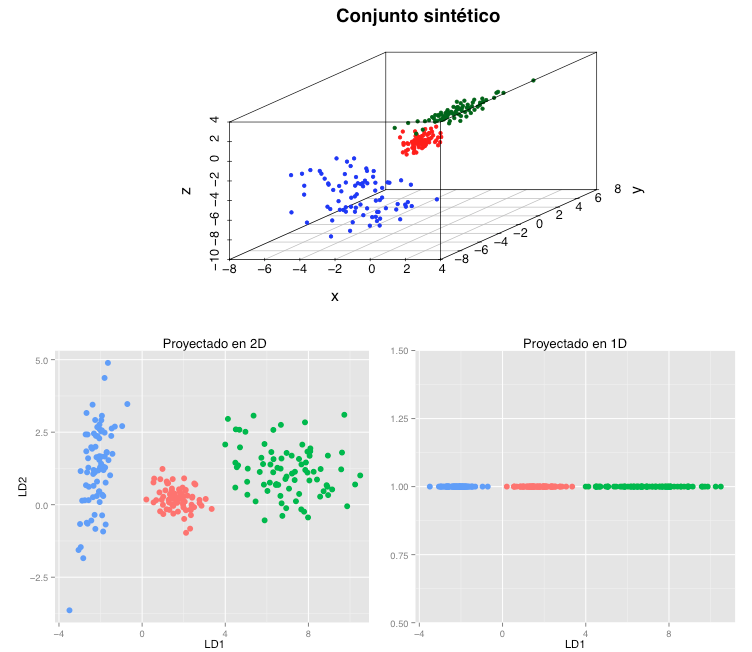
\includegraphics[width=1\textwidth]{Figures/Chapter2_1} 
  \caption[Mejores proyecciones en ${\rm I\!R}^{2}$ y ${\rm I\!R}$.]
  {En la gráfica de arriba se muestran los datos originales en 
   ${\rm I\!R}^{3}$ los cuales fueron generados a través de distribuciones normales con distintas medias y varianzas. En la gráfica de abajo a la izquierda se muestra la mejor proyección en ${\rm I\!R}^{2}$ y abajo a la derecha la mejor proyección en ${\rm I\!R}$}
\end{figure}

\subsection{Solución cuando p = 1}

El problema (1.9) toma la siguiente forma cuando $V \in {\rm I\!R}^{n}$. Se nombrara $v$ a este proyector de una dimensión ya que resulta ser solo un vector:


\begin{equation} \label{eq:2.9}
\max_{v \in {\rm I\!R}^{n}} \frac{v^T S_E v}{v^T S_I v}  
\end{equation}

Se tiene que $x_i \in {\rm I\!R}^{n}$ son los individuos originales con $i = 1 , ... , N $. Entonces sean $w_i \in {\rm I\!R}$ los individuos proyectados por el vector $v$ de manera que $w_i = v^Tx_i$. De esta manera es conveniente definir $\widehat{\mu}_k = v^T \mu_k$ y $\widehat{\mu} = v^T \mu$ como la media por clase y la media total de los datos proyectados.

\textbf{Matriz de dispersión entre clases $\Phi_{E}$ de los individuos proyectados $w_i$:}

$$\Phi_{E} = \sum\limits_{k =1}^{K} N_k (\widehat{\mu}_k - \widehat{\mu} )^2$$

$$\Phi_{E} = \sum\limits_{k =1}^{K} N_k (v^T \mu_k - v^T \mu)^2$$

$$\Phi_{E} =  \sum\limits_{k =1}^{K} N_k v^T ( \mu_k - \mu )(\mu_k - \mu )^T v $$
Por distributividad en matrices se cumple que $vAv+vBv =  v(A+B)v$, entonces:

\begin{equation}\label{eq:2.10}
\Phi_{E} = v^T \big[ \sum\limits_{k =1}^{K} N_k ( \mu_k - \mu )(\mu_k - \mu )^T \big] v	
\end{equation}

\textbf{Matriz de dispersión intra clase $\Phi_{I}$ de los individuos proyectados $w_i$}:
$$\Phi_{I} = \sum\limits_{k = 1}^{K} \sum\limits_{\substack{i = 1\\
                            y_i = k}}^{N} (w_i - \widehat{\mu}_k)^2 $$

$$\Phi_{I} = \sum\limits_{k = 1}^{K} \sum\limits_{\substack{i = 1\\
                            y_i = k}}^{N} (v_i^T x_i - v_i^T \mu_k)^{2} $$
$$\Phi_{I} =  \sum\limits_{k = 1}^{K} \sum\limits_{\substack{i = 1\\
                            y_i = k}}^{ N} v^T( x_i - \mu_k) ( x_i - \mu_k)^T v  $$

Usando de nuevo la distibutividad de matrices:

\begin{equation}\label{eq:2.11}
\Phi_{I} = v^T \big[ \sum\limits_{k = 1}^{K} \sum\limits_{\substack{i = 1\\
                            y_i = k}}^{ N} ( x_i - \mu_k) ( x_i - \mu_k)^T \big] v	
\end{equation}


 Las fórmulas de $\Phi_{I}$ y $\Phi_{E}$ de los individuos $w_i$ se pueden expresar en función de las matrices de dispersión intra clase y entre clases $S_I$ y $S_E$ de los individuos originales $x_i$. De esta manera:

 $$\Phi_{E} = f(S_E) = v^T S_E v$$
 $$\Phi_{I} = f(S_I) = v^T S_I v$$

Se tiene que $\Phi_{I}, \Phi_{E} \in {\rm I\!R}$, entonces maximizar el cociente $\frac{\Phi_{E}}{\Phi_{I}}$ con respecto a $v$ tiene como resultado una proyección que conserva cerca a los individuos pertenecientes a la misma clase, mientras que aleja a los centros de cada clase. Para el caso de una dimensión se puede encontrar una solución cerrada. La teoría asociada a este problema de maximización esta relacionada con el Cociente Generalizado de Rayleigh, el cual bajo las condiciones enunciadas de este caso, se puede transformar a un Cociente de Rayleight. Usando la proposición 1.2 se puede obtener la solución a este último.

\begin{proposition} \label{lemma2.2}
La solución a la maximización del Cociente de Rayleigh:
$$\max_{v \in {\rm I\!R}^{n} } \frac{v^T A v}{v^Tv} $$
cuando $A$ es simétrica, es obtenida cuando $v$ es el eigenvector asociado al eigenvalor más grande de la matriz $A$.
\end{proposition}


\subsection{Generalización a p dimensiones}

Para dimensiones más grandes de $v$, el Cociente Generalizado de Rayleigh no puede ser escrito en general como el Cociente de Rayleigh, por lo que la solución planteada en el capítulo anterior no es de utilidad. Esto genera la dificultad de no tener una solución cerrada, por lo que se han propuesto métodos iterativos y planteamientos alternos a la solución.

La generalización a $p$ dimensiones implica que los individuos $x_i \in {\rm I\!R}^{n}$ son proyectados ahora por la matriz $V = (V_1 | V_2 | ... |V_p)$, de manera que $w_i = V^T x_i$ con $w_i \in {\rm I\!R}^{p}$ y $V_j \in {\rm I\!R}^{n}$. De esta manera las matrices $\Phi_I$ y $\Phi_E$ se definen como sigue:

\begin{equation*}
\Phi_E = \sum\limits_{k = 1}^{K} N_{k} ||\widehat{\mu}_k - \widehat{\mu}||_2^2
\end{equation*}

\begin{equation*}
\Phi_E = \sum\limits_{k = 1}^{K} N_{k} ||V^T \mu_k - V^T \mu||_2^2
\end{equation*}

\begin{equation*}
\Phi_E = \sum\limits_{k = 1}^{K} N_{k} ||V^T (\mu_k - \mu)||_2^2
\end{equation*}


\begin{equation}\label{eq:2.17}
  \Phi_E = \sum\limits_{k = 1}^{K} N_{k} \big[ (V_1^T (\mu_k - \mu))^2 + (V_2^T (\mu_k - \mu))^2+ ... + (V_p^T (\mu_k - \mu))^2 \big]
\end{equation}

De esta expresión hay que destacar que $V_1^T (\mu_k - \mu)$ es un escalar, ya que $V_1 \in {\rm I\!R}^n$ y $(\mu_k - \mu) \in {\rm I\!R}^{n}$. Otra fórmula equivalente y que es comúnmente usada por sus propiedades algebraicas consiste en la siguiente expresión:

\begin{equation}\label{eq:2.18}
\Phi_E = \sum\limits_{k = 1}^{K} N_{k} Tr \big[ V^T (\mu_k - \mu) (\mu_k - \mu)^T V \big]	
\end{equation}

Para ejemplificarla se toma una clase $k = k_1$.  Al desarrollar $(\bullet) = V^T (\mu_1 - \mu) (\mu_1 - \mu)^T V$ se tiene una matriz en ${\rm I\!R}^{p \times p}$ igual a:


\begin{equation*}
(\bullet)= \left(\!
    \begin{array}{c}
      V_1^T (\mu_1-\mu)\\
      V_2^T (\mu_1-\mu)\\
      \vdots \\
      V_p^T (\mu_1-\mu)
    \end{array}
  \!\right) 
  \left(\!\begin{array}{c}
      (\mu_1-\mu)^T V_1 \quad
      (\mu_1-\mu)^T V_2 \quad
      \hdots \quad
      (\mu_1-\mu)^T V_p
    \end{array}
  \!\right) 
\end{equation*} 

\vspace{5mm}

\begin{equation*}
(\bullet)= \left(\!
    \begin{array}{ccc}
      V_1^T (\mu_1-\mu) (\mu_1-\mu)^T V_1 & \hdots & V_1^T (\mu_1-\mu) (\mu_1-\mu)^T V_p  \\
      V_2^T (\mu_1-\mu) (\mu_1-\mu)^T V_1 & \hdots & V_2^T (\mu_1-\mu) (\mu_1-\mu)^T V_p  \\
      \vdots & \ddots & \vdots\\
      V_p^T (\mu_1-\mu) (\mu_1-\mu)^T V_1 & \hdots & V_p^T (\mu_1-\mu) (\mu_1-\mu)^T V_p
    \end{array}
  \!\right) 
\end{equation*} 

\vspace{5mm}

\begin{equation*}
(\bullet)= \left(\!
    \begin{array}{ccc}
      (V_1^T (\mu_1-\mu))^2 & \hdots & V_1^T (\mu_1-\mu) (\mu_1-\mu)^T V_p \\
       V_2^T (\mu_1-\mu) (\mu_1-\mu)^T V_1  & \hdots & V_2^T (\mu_1-\mu) (\mu_1-\mu)^T V_p  \\
      \vdots & \ddots & \vdots\\
      V_p^T (\mu_1-\mu) (\mu_1-\mu)^T V_1  & \hdots & (V_p^T (\mu_1-\mu))^2
    \end{array}
  \!\right) 
\end{equation*} 

\vspace{5mm}

 Por lo tanto al calcular la traza de la matriz de $p \times p$ desarrollada arriba, se tiene que $Tr(V^T (\mu_1 - \mu) (\mu_1 - \mu)^T V)$ es equivalente a:
 \vspace{3mm}
 \begin{equation*}
Tr(\bullet) = (V_1^T (\mu_1-\mu))^2+ (V_2^T (\mu_1-\mu) )^2 + \hdots + (V_p^T (\mu_1-\mu) )^2
 \end{equation*}

Al generalizar a las $K$ clases y usando la propiedad de linealidad en la traza; es decir, $Tr(A+B) = Tr(A)+Tr(B)$, entonces se puede escribir de la siguiente manera:

\begin{equation*}
\Phi_E = Tr \sum\limits_{k = 1}^{K} N_{k}  \big[ V^T (\mu_k - \mu) (\mu_k - \mu)^T V \big]
\end{equation*}


Esta expresión es equivalente a (1.16). Como paso final se factoriza $V^T$ y $V$ sobre todos los sumandos, lo que nos llevaría a lo siguiente:

\begin{equation*} 
\Phi_E =  Tr (V^T \sum\limits_{k = 1}^{K} N_{k}  \big[(\mu_k - \mu) (\mu_k - \mu)^T \big] V)   
\end{equation*}

o, expresada en términos de $S_E = \sum\limits_{k = 1}^{K} N_{k}  \big[(\mu_k - \mu) (\mu_k - \mu)^T \big]$

\begin{equation}\label{eq:2.19}
\Phi_E =  Tr (V^T S_E V)     
\end{equation}

Similarmente se puede llegar a la formulación de la varianza intra-clase $\Phi_{I}$.
\begin{equation}\label{eq:2.20}
\Phi_{I} =  Tr (V^T S_I V )
\end{equation}



\subsection{Existencia de la solución}

Para demostrar la existencia y unicidad de la solución, las matrices $S_I$ y $S_E$ deben cumplir ciertas características. Sean $A = S_E$ y $B = S_I$, la primer condición que se les impone es que sean positivas definidas. La razón que apoya la restricción está relacionada con la forma de la función a maximizar, que es un cociente. Como $B$ se encuentra en el denominador, se tiene que evitar que $Tr(V^T B V) = 0$, ya que con este valor se indetermina la función objetivo \cite{ngo2012trace}. 

T.T. Ngo propone generalizar el estudio a las matrices positivas semidefinidas. Para esto se deben encontrar los casos en que $Tr(V^T B V)$ toma el valor de $0$. Si se diagonaliza a la matriz $B = Q \Lambda_{B} Q^T$ con $Q$ ortogonal y $\Lambda_{B}$ una matriz diagonal con entradas iguales a los eigenvalores de $B$, entonces:

\begin{equation*}
Tr(\Lambda_{B}) = \lambda_{B_1}+ \lambda_{B_2}+ ... +\lambda_{B_n} \qquad con \qquad \widehat{V} = Q^T V
\end{equation*}



De este modo $\widehat{V} = (\widehat{V}_1 | \widehat{V}_2 | ... | \widehat{V}_p)$ y cada $\widehat{V}_i^T = (\widehat{V}_{i1}, \widehat{V}_{i2}, ..., \widehat{V}_{in})$ es un vector renglón. De esta manera la matriz $\widehat{V}^T$:

\begin{equation*}
\widehat{V}^T = 	
\left(\!
    \begin{array}{c}
      \widehat{V}_1^T\\
      \widehat{V}_2^T\\
      \vdots \\
      \widehat{V}_p^T
    \end{array}
  \!\right)   = 
\left(\!
    \begin{array}{cccc}
      \widehat{V}_{11} & \widehat{V}_{12} & \hdots & \widehat{V}_{1n}\\
      \widehat{V}_{21} & \widehat{V}_{22} & \hdots & \widehat{V}_{2n}\\
      \vdots &  \vdots &\ddots & \vdots\\
      \widehat{V}_{p1} & \widehat{V}_{p2} & \hdots & \widehat{V}_{pn}\\
    \end{array}
  \!\right) 
\end{equation*}

Por lo que la traza que involucra a $B$ tiene la siguiente forma:

\begin{equation*}
Tr(V^T B V) = Tr(V^T Q \Lambda_{B} Q^T V) 	
\end{equation*}

\begin{equation*}
Tr(V^T B V)  = Tr(\widehat{V}^T \Lambda_{B} \widehat{V})
\end{equation*}

\begin{equation*}
V^T B V = 
\left(\!
    \begin{array}{c}
      \widehat{V}_1^T\\
      \widehat{V}_2^T\\
      \vdots \\
      \widehat{V}_p^T
    \end{array}
  \!\right) 
  \left(\!
    \begin{array}{cccc}
      \lambda_{B_1} & 0 & \hdots & 0\\
      0 & \lambda_{B_2} & \hdots & 0\\
      \vdots &  \vdots &\ddots & \vdots\\
      0 & 0 & \hdots & \lambda_{B_n}\\
    \end{array}
  \!\right) 
  \left(\!\begin{array}{c}
      \widehat{V}_1 |
      \widehat{V}_2 |
      \hdots |
      \widehat{V}_p
    \end{array}
  \!\right) 
\end{equation*} 

Desarrollando la multiplicación de matrices, y calculando la traza resulta en los siguientes sumandos:
 
 \begin{equation*}
\begin{aligned}
      Tr(V^T B V) =& \lambda_{B_1} \widehat{V}_{11}^2&  +
                     & \lambda_{B_2} \widehat{V}_{12}^2& +
                     & \hdots& +
                     &\lambda_{B_n} \widehat{V}_{1n}^2& + \\
                     & \lambda_{B_1} \widehat{V}_{21}^2&+
                     & \lambda_{B_2} \widehat{V}_{22}^2& +
                     & \hdots& +
                     &\lambda_{B_n} \widehat{V}_{2n}^2& + \\
                     & \vdots&  
                     & \vdots& 
                     & \vdots& 
                     & \vdots& \\
                     & \lambda_{B_1} \widehat{V}_{p1}^2&+
                     & \lambda_{B_2} \widehat{V}_{p2}^2& +
                     & \hdots& + 
                     & \lambda_{B_n} \widehat{V}_{pn}^2.&  
 \end{aligned}
 \end{equation*}

 Es fácil de ver que la expresión de arriba tiene $p \times n$ sumandos, por lo que se puede expresar en términos de dos sumatorias. La primera de $j=1,...,p$ y la segunda de $i = 1,...n$:

\begin{equation*} 
Tr(V^T B V) = \sum \limits_{j=1}^{p} \sum\limits_{i=1}^{n} \lambda_{B_i} \widehat{V}_{ji}^2
\end{equation*}

\begin{equation}\label{eq:2.21}
Tr(V^T B V) = \sum\limits_{i=1}^{n} \lambda_{B_i} \sum \limits_{j=1}^{p} \widehat{V}_{ji}^2    
\end{equation}

De la última expresión se separa la sumatoria sobre $i$. De esta manera, para cada elemento $i$ se tienen dos factores:

\begin{equation}\label{eq:2.22}
(i) \lambda_{B_i}
\end{equation}

 \begin{equation}\label{eq:2.23}
 (ii) \sum \limits_{j=1}^{p} \widehat{V}_{ji}^2   
 \end{equation}
 

 La idea para que $Tr(V^T B V)$ sea positivo, es que al menos uno de los sumandos sea positivo. Si (1.21) y (1.22) son ambos distintos de cero para al menos una $i$, entonces se cumple esta condición. Esta idea está expresada en el Lema 1.1.

\begin{lemma}\label{lemma2.4}
Sea $B$ positiva semidefinida y $V \in {\rm I\!R}^{n\times p}$. Si $B$ tiene a lo más $p-1$ eigenvalores iguales a $0$, entonces $Tr(V^T B V)  = Tr(\widehat{V}^T \Lambda_{B} \widehat{V}) \neq 0$  para cualquier matriz ortogonal $V$.
\end{lemma}

\begin{proof}
Sea $\widehat{V} = [\widehat{V}_1 | ... | \widehat{V}_p]$ tal que $\widehat{V} \widehat{V} = V^T Q Q^T V = V^T I_n V  = I_p$. De esta manera se puede construir una matriz $\widehat{V}' \in {\rm I\!R}^{p \times p}$ seleccionando $p$ de los $n$ renglones de $\widehat{V}$ tal que $\widehat{V}'$ sea no singular. $\widehat{V}'$ tiene la propiedad de no contener eigenvalores iguales a 0; como consecuencia, sus renglones y columnas no contienen al vector $\widehat{0}$. Al no contenerlo,se sabe que al menos hay $p$ renglones de $\widehat{V}$ tal que $\sum_{j=1}^{p}\widehat{V}_{ji}^2 \neq 0$ para cada uno de ellos. Por otra parte en el lema se supone que la matriz $B$ tiene a lo más $p-1$ eigenvalores iguales $0$ por lo que al menos un elemento de la sumatoria es distinto de cero.
\end{proof}

Analizando a mayor profundidad el resultado anterior, se sabe que hay $n-p+1$ eigenvalores de $B$ positivos ($\lambda_{B_i} \neq 0$) y $p$ renglones de $\widehat{V}$ que tienen norma distinta de cero. Al calcular la sumatoria (1.20), se tiene que al menos una combinación de $\lambda_{B_i}$ y uno de los $p$ renglones cumplen que su multiplicación tiene signo positivo. Para ejemplificar esta situación sean $C_i$ con $i = 1, ... , n-p+1$ los eigenvalores de $B$ y $K_j$ con $j = 1, ... , p$ la norma de los renglones de $\widehat{V}$ que son distintos de $0$.
 
\begin{center}
\begin{tabular}{ | c | c|  c | c|} 
\hline
$i$ & $\lambda_{B_i}$ & $\sum \limits_{j=1}^{p} \widehat{V}_{ji}^2$  & $\lambda_{B_i} \sum \limits_{j=1}^{p} \widehat{V}_{ji}^2$ \\ 
\hline
\hline
1 & $C_1$ & $0$ & $0$ \\ 
\hline
2 & $C_2$ & $0$ & $0$ \\ 
\hline
\vdots & \vdots & \vdots & \vdots \\ 
\hline
$n-p$ & $C_{n-p}$ & $0$ &  $0$\\ 
\hline
$n-p+1$ & $C_{n-p+1}$ & $K_{p}$ &  $C_{n-p+1} K_{p}$\\ 
\hline
$n-p+2$ & $0$ & $K_{p-1}$  & $0$ \\ 
\hline
\vdots & \vdots & \vdots & \vdots  \\ 
\hline
$n-1$ & $0$ & $K_2$ & $0$ \\ 
\hline
$n$ & $0$ & $K_1$ & $0$ \\ 
\hline
\hline

\end{tabular}
\end{center}

Con esta combinación se tiene que al menos hay un sumando de $\sum\limits_{i=1}^{n} \lambda_{B_i} \sum \limits_{j=1}^{p} \widehat{V}_{ji}^2 $ distinto de cero, por lo que $Tr(V^T B V) \neq 0$. Bajo estas condiciones se garantiza que el denominador sea mayor a 0, solo falta asegurarse que el numerador sea menor a infinito.

\begin{lemma}
Sea $U_p = \{ V \in {\rm I\!R}^{n \times p} | V^T V = I_p \} $ un conjunto compacto con $V = (v_1, v_2, ... , v_p)$
\end{lemma}
\begin{proof}
Se tiene que $U_p$ es un conjunto cerrado porque contiene a todos sus puntos límite; por otro lado, $U_p$ también es acotado bajo la norma 2 y la norma de Frobenius:

Tomando la norma-2 y la norma de Frobenius de $V$: 
\begin{equation*}
\begin{aligned}
	||V||_2 =& Max \{||V_x ||_2 \quad | \quad ||x||_2 = 1 \} \\
		    =& ||V_x||^2_2  \\
		    =& (Vx)^T (Vx) \\
		    =& x^T V^T V x\\
		    =& x^T x = 1\\
	||V||_F	=& \sum\limits_{F}^{p} ||v_i|| = p   
\end{aligned}
\end{equation*}

Entonces se tiene $U_p$ es cerrado y acotado, por lo que $U_p$ es compacto.
\end{proof}

Con este resultado se tiene que $Tr(V^T A V)$ toma un valor finito ya que todas sus entradas son finitas. 


\begin{lemma}\label{lemma2.5}
Sean $A$ y $B$ dos matrices simétricas tales que $B$ es positiva semidefinida con rango mayor que $n-p$; es decir, que tenga al menos $n-p+1$ eigenvalores distintos de cero. Entonces el cociente $(1.9)$ admite un máximo con valor $\rho^*$ \cite{ngo2012trace}.
\end{lemma}

\begin{proof}
Tomando el resultado del lema 1.1 se tiene que $Tr(V^T B V) \neq 0$; por otra parte, $V \in U_p$ que es un conjunto compacto. Con estas dos observaciones, el valor de (1.9) es distinto de infinito. Entonces el cociente $(1.9)$ admite un máximo con valor $\rho^*$ y que tiene como argumento $V^{**}$.
\end{proof}

\subsection{Equivalencia con un problema escalar}

\textbf{Valor en el óptimo}. Del lema 1.3 se sabe que existe una matriz $V^{**} \in U_p$ tal que (1.9) alcanza el valor máximo $\rho^*$. Expresando esta idea se tiene que:

\begin{equation} \label{eq:2.24}
 \frac{Tr(V^{T**} A V^{**})}{Tr(V^{T**} B V^{**})} = \rho^* 
\end{equation}

Entonces para cualquier otra matriz $V \in U_p $:

\begin{equation}\label{eq:2.25}
 \frac{Tr(V^T A V)}{Tr(V^T B V)} \leq \rho^* 
\end{equation}

Como la traza es un operador lineal y por la propiedad distributiva de las matrices entonces (1.24) es equivalente a:

\begin{equation*}
 Tr(V^T A V)- \rho^* Tr(V^T B V) \leq 0 
\end{equation*}

\begin{equation*}
	Tr(V^T A V- \rho^* V^T B V) \leq 0	
 \end{equation*}

 \begin{equation} \label{eq:2.26}
	Tr(V^T (A - \rho^* B )V) \leq 0	
 \end{equation}

y el resultado equivalente para (1.23):
	
 \begin{equation} \label{eq:2.27}
	Tr(V^{T**} (A - \rho^* B )V^{**}) = 0	
 \end{equation}


Para facilitar la lectura, de aquí en adelante se define la función $G(\rho) = A- \rho B$. Maximizar el lado izquierdo de la desigualdad (1.25) sujeto a $V^T V = I$ es equivalente a maximizar un problema de eigenvalores generalizado. Usando lo establecido en el apéndice A, se sabe que el valor máximo de este problema dado $\rho^*$:

\begin{equation}\label{eq:2.28}
	\max_{\substack{V \in {\rm I\!R}^{n \times p} \\ V^T V = I}} Tr(V^T G(\rho^*) V) = \lambda_{G(\rho^*)_1} + \lambda_{G(\rho^*)_2} + ... + \lambda_{G(\rho^*)_p}
\end{equation}
  
 Con $\lambda_{G(\rho^*)_1} \geq \lambda_{G(\rho^*)_2} \geq ... \geq \lambda_{G(\rho^*)_p}$ los $p$ eigenvalores más grandes de $G(\rho^*)$. De esta manera el valor óptimo de (1.27) es simplemente la suma de los $p$ eigenvalores más grandes de esta matriz, y $V^{**}$ el conjunto de correspondientes eigenvectores. Para obtener este valor y la matriz, el primer paso es encontrar a $\rho^*$, ya que teniéndolo es inmediato calcular $V^{**}$. Dada esta premisa, se puede ver que el problema a resolver se reduce a buscar el valor óptimo de $\rho$. Para esto se define la función $f(\rho)$ sobre todo $\rm I\!R$, tal que $f(\rho)$ es continua sobre su argumento $\rho$: 

\begin{equation}  \label{eq:2.29}
	f(\rho) = \max_{V^T V = I} Tr(V^T (G(\rho)) V)
\end{equation}

Es conveniente examinar $f(\rho)$ con dos objetivos, el primero es estimar la dificultad de calcular el valor de $f(\rho)$ y el segundo es encontrar la maximización adecuada para obtener $\rho^*$. Respecto al primer punto, la manera de calcular $f(\rho)$ en cada punto es equivalente a (1.27), pero en lugar de usar los eigenvalores de $G(\rho^*)$ se usan los de $G(\rho)$. En particular se llamará $V(\rho)^*$ al argumento que resuelve (1.28) \footnote{Se utilizó la nomenclatura de $V(\rho^*)$ porque estos eigenvectores dependen del valor de $\rho$ en la matriz $A - \rho B$.}. Sean $\lambda_{G(\rho)_1} \geq \lambda_{G(\rho)_2} \geq ... \geq \lambda_{G(\rho)_n}$ los $n$ eigenvalores de $G(\rho)$. Con esta notación $f(\rho)$ toma el valor de:


\begin{equation}\label{eq:2.30}
f(\rho) = \lambda_{G(\rho)_1} + \lambda_{G(\rho)_2} + ... +\lambda_{G(\rho)_p}
\end{equation}


Para el segundo punto, la idea es iterar hasta obtener el valor de $\rho^*$. Por esto, es conveniente analizar como se comporta la función con respecto a su argumento. A continuación se presentan dos propiedades de $f(\rho)$. Para demostrarlas, primero se enuncia el teorema 8.1.5 de \cite{golub2012matrix}.

\begin{theorem} \label{teorem.1}
	
	Sean $X$ y $X+E$ matrices simétricas $n \times n$, y $\lambda_{X_k}$, $\lambda_{E_k}$ los k-ésimos eigenvalores más grandes de $X$ y $E$ respectivamente. De esta manera $\lambda_{X_k}$ es el k-ésimo eigenvalor más grande de $X$ y $\lambda_{E_1}$ el más grande de $E$. Con estas definiciones se cumple lo siguiente:

	\begin{equation}\label{eq:2.31}
		\lambda_{X_k} +\lambda_{E_n} \leq \lambda_{(X+E)_k} \leq \lambda_{X_k} +\lambda_{E_1}
	\end{equation}

\end{theorem}

Se procede a enunciar este lema acerca de la función $f(\rho)$

\begin{lemma}\label{lemma2.6}
La función $f(\rho) = \max_{V^T V = I} Tr(V^T (A - \rho B) V)$ cumple las siguientes dos propiedades: 

(1) $f$ es una función no creciente de $\rho$ \\
(2) $f(\rho)= 0$  si y solo si $\rho = \rho^*$
\end{lemma}

Para probar la parte $(1)$ del lema 1.4 se comparan los valores de $f(\rho)$ para $\rho_1$ y $\rho_2$ con $\rho_2 \geq \rho_1$. Como se desea demostrar que $f$ es una función no creciente de $\rho$, se busca que $f(\rho_2) \leq f(\rho_1)$. Se definen las matrices $Y=X+E$ y $E = Y-X$, para después restarles $\lambda_{X_k}$, entonces (1.29) se puede escribir como:

\begin{equation*}
		\lambda_{(X)_k} +\lambda_{(Y-X)_n} \leq \lambda_{(Y)_k} \leq \lambda_{(X)_k} +\lambda_{(Y-X)_1}
\end{equation*}

\begin{equation*}
		\lambda_{(Y-X)_n} \leq \lambda_{(Y)_k} - \lambda_{(X)_k} \leq \lambda_{(Y-X)_1}
\end{equation*}

La expresión en el centro de estas desigualdades es la resta del eigenvalor k-ésimo de la matriz $X$ y $Y$, por lo que si se realiza la suma de $k = 1$ a $k = p$ se tiene lo siguiente:

\begin{equation}\label{eq:2.32}
		p \lambda_{(Y-X)_n} \leq \sum_{k=1}^{p} \lambda_{(Y)_k} - \sum_{k=1}^{p} \lambda_{(X)_k} \leq  p \lambda_{(Y-X)_1}
\end{equation}

Definiendo $X = A - \rho_2 B$ y $Y = A - \rho_1 B$, entonces (1.31) toma la siguiente forma:

\begin{equation}\label{eq:2.33}
    p \lambda_{(B(\rho_2-\rho_1))_n} \leq \sum_{k=1}^{p} \lambda_{(A - \rho_1 B)_k} - \sum_{k=1}^{p} \lambda_{(A - \rho_2 B)_k} \leq  p \lambda_{(B(\rho_2-\rho_1))_1}
\end{equation}

Retomando el resultado (1.29), y sustituyéndolo en (1.32) la desigualdad queda de la siguiente forma:

\begin{equation}\label{eq:2.34}
		p \lambda_{(B (\rho_2 - \rho_1))_n} \leq f(\rho_1) - f(\rho_2) \leq  p \lambda_{(B (\rho_2 - \rho_1))_1}
\end{equation}


En la parte izquierda de la desigualdad anterior, se puede a determinar el signo que toman los eigenvalores $\lambda_{(B (\rho_2 - \rho_1))_n}$. 
Si $(\rho_2- \rho_1) \geq 0$ entonces la matriz $(\rho_2 - \rho_1)B$ es positiva semidefinida; por lo tanto, todos sus eigenvalores son mayores o iguales a 0:

\begin{equation*}
	0 \leq p \lambda_{(B (\rho_2 - \rho_1))_n} \leq f(\rho_1) - f(\rho_2) \leq  p \lambda_{(B (\rho_2 - \rho_1))_1}
\end{equation*}
	
\begin{equation}\label{eq:2.35}
	0 \leq f(\rho_1) - f(\rho_2)
\end{equation}

De esta manera $f(\rho_2)  \leq  f(\rho_1) $ cuando $\rho_2 \geq \rho_1$

Para probar la parte (2) del lema 1.4, se tiene que demostrar la condición suficiente y la condición necesaria. La demostración de la primera es inmediata, ya que cuando $\rho = \rho^*$, entonces por (1.26), $f(\rho) = 0$. Para la condición necesaria se usará (1.23) y la propiedad que la $Tr(V^T B V) >0 \enspace \forall \enspace V \in U_p$. Se demostrará que, dado $f(\rho^*) = 0$, entonces:


\begin{equation}\label{eq:2.36}
	(i) \quad f(\rho) < 0 \quad si \quad \rho>\rho^*
\end{equation}
\begin{equation}\label{eq:2.37}
	(ii) \quad f(\rho) > 0 \quad si \quad \rho<\rho^*
\end{equation}

\underline{\textbf{Caso (i) $\rho > \rho^* $}}

Se tiene que las siguientes desigualdades se cumplen:
\begin{equation*}
\frac{Tr(V^T A V)}{Tr(V^T B V)} \leq \rho^* < \rho	
\end{equation*}

Por lo que es equivalente a:

\begin{equation*}
	Tr(V^T (A -\rho B)V) < 0 \quad \forall V \in U_p
\end{equation*}


De esta manera $f(\rho) < 0$ cuando $\rho > \rho^*$.
\vspace{5mm}

\underline{\textbf{(ii) $\rho < \rho^* $}}

Retomando el resultado (1.24) y suponiendo que $\rho^* > \rho$ entonces existe una $V^{*}$ tal que:


 \begin{equation*} 
 \rho < \frac{Tr(V^{T*} A V^*)}{Tr(V^{T*} B V^*)} \leq \rho^*
 \end{equation*}

\begin{equation*}
Tr(V^{T*} A V^* - \rho V^{T*} B V^*) > 0 \quad \Longrightarrow \quad \frac{Tr(V^{T*} A V^*)}{Tr(V^{T*} B V^{*})} > \rho
\end{equation*}

En particular:

\begin{equation*}
\max_{V^TV} \frac{Tr(V^{T} A V)}{Tr(V^{T} B V)} > \rho
\end{equation*}

De esta manera $f(\rho) > 0$ cuando $\rho < \rho^*$.


Las ecuaciones (1.35) (1.36), junto con la continuidad de la funcion $f$, muestran que $f(\rho) = 0$ implica $\rho = \rho^*$ \cite{ngo2012trace}. De esta manera el problema puede ser visto como encontrar la raíz de la función $f(\rho)$. La figura 1.4 muestra como es esta función.

\begin{corollary}
La función $f(\rho) = \max_{V^TV = I} Tr(V^T (A -\rho B)V)$ cumple las siguientes condiciones:

$$f(\rho) > 0  \quad \forall \quad \rho \in (-\inf, \rho^*)$$
$$f(\rho) < 0  \quad \forall \quad \rho \in (\rho^*, \inf)$$

\end{corollary}

\begin{figure}[!ht]\label{Fig1.3}
  \centering
	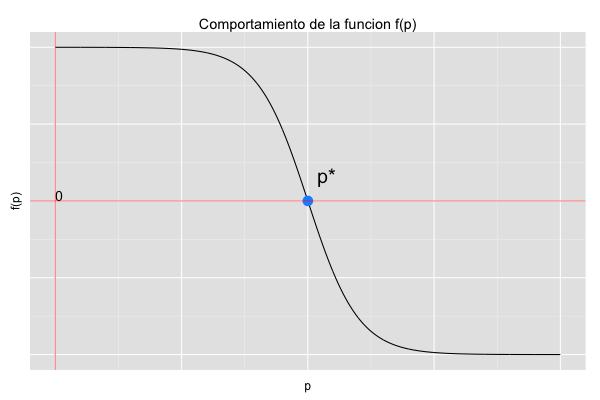
\includegraphics[width=1\textwidth]{Figures/Chapter2_fp}	
  \caption[Comportamiento de $f(\rho)$.]
  {La función $f(\rho)$ es no creciente para toda $\rho$. El valor de $f(\rho) = \lambda_{G(\rho)1}+ \lambda_{G(\rho)2} + ... +\lambda_{G(\rho)p}.$ $f(\rho^*) = 0 $}
\end{figure}


\begin{example} \label{ex:1}
Para ejemplificar el lema 1.4 se muestran las matrices $A,B \in {\rm I\!R}^{3 \times 3}$. Para el valor de $f(\rho)$ se utiliza la propiedad (1.29):

$$f(\rho) = \lambda_{G(\rho)1} + \lambda_{G(\rho)2} + ... + \lambda_{G(\rho)p}$$

con $p$ la dimensión a la que se va a proyectar. 


\begin{equation*}
A = \left(\!
    \begin{array}{ccc}
      4 & 0 & 0 \\
      0 & 6 & 0 \\
      0 & 0 & 8 
    \end{array}
  \!\right), \quad
B = \left(\!
    \begin{array}{ccc}
      1.5 & 0 & 0 \\
      0 & 2.5 & 0 \\
      0 & 0 & 5 
    \end{array}
\!\right) 
\end{equation*}



\begin{equation*}
G(\rho) = A- \rho B = \left(\!
    \begin{array}{ccc}
      4-1.5\rho & 0 & 0 \\
      0 & 6-2.5\rho & 0 \\
      0 & 0 & 8-5\rho 
    \end{array}   	
      \!\right) 
\end{equation*}

Los eigenvalores de esta matriz son $4-1.5\rho$,  $6-2.5\rho$ y  $8-5\rho$. Las funciones graficadas de estos eigenvalores se presentan en la figura 1.5.

\begin{figure}[!ht] \label{Fig1.4}
  \centering
  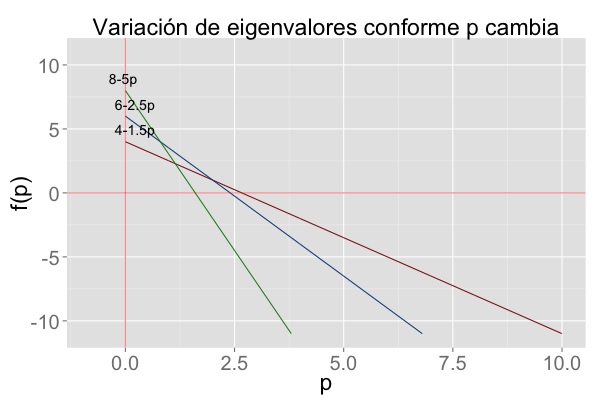
\includegraphics[width=1\textwidth]{Figures/Chapter2_3eigen}  
  \caption[Gráfica de los eigenvalores en función de $\rho$.] {Cada línea representa como se comporta cada eigenvalor de $A- \rho B$ cuando se varía $\rho$.}
\end{figure}

Cuando se desea que el proyector sea de dimensión 1, entonces se tiene que $f(\rho)$ es el eigenvalor más grande,  cuando sea de dimensión 2, la suma de los dos más grandes y así respectivamente. El valor de $f(\rho)$ para estos tres casos está representado en la figura 1.5.

\begin{figure}[!ht] \label{Fig1.5}
  \centering
  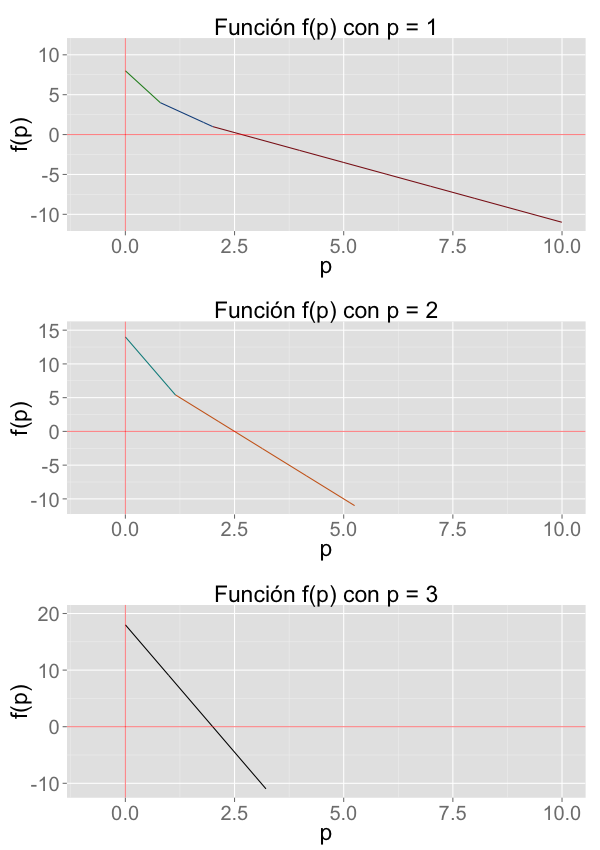
\includegraphics[width=1\textwidth]{Figures/Chapter2_grid3eigen}  
  \caption[$f(\rho)$ para proyectores de 1,2 y 3 dimensiones.] {La figura superior representa a $f(\rho) = \lambda_{G(\rho)_1}$, la de enmedio $f(\rho) = \lambda_{G(\rho)_1} + \lambda_{G(\rho)_2}$ y la de abajo $f(\rho) = \lambda_{G(\rho)_1} + \lambda_{G(\rho)_2} + \lambda_{G(\rho)_3}$.}
\end{figure}

\end{example}
\pagebreak

\subsection{Localización del óptimo}

En la sección anterior se encontró que la maximización al cociente de trazas puede ser visto como el problema de encontrar la raíz de la función $f(\rho) = max_{V^T V= I} Tr(V^T(A-\rho B)V)$. Por esto, encontrar un intervalo $(\rho_1, \rho_2)$ que contenga al valor óptimo $\rho^*$ puede reducir el número de iteraciones del método. Usando el lema 1.4 se sabe que $f$ es una función no creciente de $\rho$. Por esta razón si se encuentra una $\rho_1$ y $\rho_2$ tal que $f(\rho_1) \geq 0$ y $f(\rho_2) \leq 0$ y con la propiedad de continuidad de la funcion $f(\rho)$ entonces se encontró un intervalo que contiene a $\rho^*$. 

En esta tesis se dan cotas para el valor de $\rho^*$, la primera en función los eigenvalores de una transformación de $B -\rho A$ y la segunda en función de los eigenvalores de $B$ y $A$ \cite{ngo2012trace}. La demostración de cada una requiere del conocimiento del concepto de inercia y del Teorema de la Inercia de Sylvester. Por este motivo se presentan a continuación: \footnote{La demostración de este teorema puede ser encontrada en \cite{golub2012matrix}.}

\begin{definition}
La inercia de una matriz simétrica $A$ es la tripleta de enteros no negativos $(m, z, p)$ donde $m$, $z$ y $p$ son respectivamente el número de eigenvalores negativos, cero y positivos de $A$ \cite{golub2012matrix}.
\end{definition}

\begin{theorem}\label{teorem.2}
Sea $A \in {\rm I\!R}^{n \times n}$ una matriz simétrica y $Z \in {\rm I\!R}^{n \times n}$ no singular. Entonces $A$ y $Z^T A Z$ tienen la misma inercia \cite{golub2012matrix}.
\end{theorem}

\begin{proposition}
La raíz $\rho^*$ de $f(\rho)$ está localizada en el intervalo $(\lambda_p, \lambda_1)$ donde $\lambda_p$ es el p-ésimo eigenvalor más grande de $Z^T(A-\rho B)Z$.
\end{proposition}

\begin{proof}
Sea $Z$ la matriz que diagonaliza a $A-\rho B$ de manera que\footnote{El cálculo de esta matriz puede obtenerse en el algoritmo 8.7.1 de \cite{golub2012matrix}}:

\begin{equation}\label{eq:2.38}
\begin{aligned}
 Z^T AZ = \Lambda \\ Z^T B Z = I
 \end{aligned}
\end{equation}

Con $\Lambda$ una matriz diagonal y $\mu_1, \ldots,  \mu_n$ sus respectivos eigenvalores e $I$ la identidad de tamaño $n$. Entonces por el teorema 1.2 se sabe que $A- \rho B$ y $Z^T(A- \rho B)Z = \Lambda -\rho I$ tienen el mismo número de eigenvalores positivos, negativos y cero. Por lo tanto, la matriz en cuestión es de la siguiente forma:

\begin{equation}\label{eq:2.39}
\Lambda - \rho I = 
\left(\!
    \begin{array}{cccc}
      \mu_1 & 0 & \hdots & 0\\
      0 & \mu_2 & \hdots & 0\\
      \vdots & \vdots & \ddots & \vdots \\
      0 & 0 & \hdots & \mu_n
    \end{array}
  \!\right) - \rho
  \left(\!
    \begin{array}{cccc}
      1 & 0 & \hdots & 0\\
      0 & 1 & \hdots & 0\\
      \vdots & \vdots & \ddots & \vdots \\
      0 & 0 & \hdots & 1
    \end{array}
  \!\right) 
\end{equation} 

Como la  matriz $V$ de (1.9) es de tamaño $n \times p$, solo nos interesa saber el signo de los $p$ eigenvalores más grandes. Tomando $\rho = \mu_p$ entonces los elementos de la diagonal de la matriz $\Lambda- \rho I$ son de la forma:


\begin{equation}\label{eq:2.40}
\begin{aligned}
   \mu_i - \mu_p & \geq 0  \quad para \quad i \geq p\\
   \mu_i - \mu_p & \leq 0  \quad para \quad i \leq p
\end{aligned}
\end{equation} 

Los primeros p elementos tienen la propiedad de ser no negativos, ya que $\lambda_{(A-\rho B)_1} \geq \lambda_{(A-\rho B)_2} \geq ... \geq \lambda_{(A-\rho B)_p}$. Usando el teorema 1.2 se sabe que los primeros p eigenvalores de $A-\rho B$ también son no negativos. Por ende la suma de ellos es mayor o igual que cero. 

Por otro lado si se toma $\rho = \mu_1$. Entonces los elementos de la diagonal de la matriz (1.38) son de la forma:

\begin{equation}\label{eq:2.41}
   \mu_i - \mu_1  \leq 0 \quad \forall \quad i
\end{equation} 

Con $i = 1, ..., p$, cada uno de los elementos de la diagonal tiene la propiedad de ser no positivo por el mismo argumento que el caso pasado. Por lo tanto los $p$ eigenvalores más grandes de $\Lambda - \rho I$ y de $A-\rho B$ son no positivos, por lo que su suma es menor o igual que cero:

\begin{equation}\label{eq:2.42}
  \rho = \mu_p  \Rightarrow \sum_{i=1}^{p} (\mu_i- \mu_p) \geq 0 \Rightarrow f(\rho) \geq 0
\end{equation}

\begin{equation}\label{eq:2.43}
  \rho = \mu_1  \Rightarrow \sum_{i=1}^{p} (\mu_i - \mu_1) \leq 0 \Rightarrow f(\rho) \leq 0
\end{equation}

\end{proof}

\pagebreak

\begin{example} \label{ex:2}
Tomando las matrices A,B iguales que en el ejercicio 1.1, se puede encontrar fácilmente a la matriz $Z$:


\begin{equation*}
Z = \left(\!
    \begin{array}{ccc}
      \sqrt(\frac{1}{1.5}) & 0 & 0 \\
      0 & \sqrt(\frac{1}{2.5}) & 0 \\
      0 & 0 & \sqrt(\frac{1}{5}) 
    \end{array}
  \!\right)
\end{equation*}

Con la matriz $Z$ definida de esta manera, $Z^T A  Z = \Lambda$ y $Z^T B Z = I$ toman la siguiente forma:

\begin{equation*}
\Lambda - \rho I = 
\left(\!
    \begin{array}{ccc}
      \frac{4}{1.5} & 0  & 0\\
      0 & \frac{6}{2.5}  & 0\\
      0 & 0 & \frac{8}{5}
    \end{array}
  \!\right) - \rho
  \left(\!
    \begin{array}{ccc}
      1 & 0 & 0\\
      0 & 1 & 0\\
      0 & 0 & 1
    \end{array}
  \!\right) 
\end{equation*}

Entonces se puede encontrar un intervalo tal que $\rho^* \in \big[\rho_1, \rho_2 \big]$:

\begin{equation*}
  \begin{aligned}
\rho_1 &= \mu_p \\
\rho_2 &= \mu_1  
  \end{aligned}
\end{equation*}

Conforme el tamaño de la dimensión a proyectar cambia, las cotas son las siguientes:

\begin{equation*}
  \begin{aligned}
  p =& 1 \Rightarrow \qquad \rho_1 = \frac{4}{1.5} \quad y \quad \rho_2 = \frac{4}{1.5}\\
  p =& 2 \Rightarrow \qquad \rho_1 = \frac{4}{1.5} \quad y \quad \rho_2 = \frac{6}{2.5} \\
  p =& 3 \Rightarrow \qquad \rho_1 = \frac{4}{1.5} \quad y \quad \rho_2 = \frac{8}{5}
  \end{aligned}
\end{equation*}
 

 Estas cotas se pueden ver más fácil en la figura 1.6,donde se observa $f(\rho)$ con respecto a $p$:

\begin{figure}[!ht] \label{Fig1.6}
  \centering
  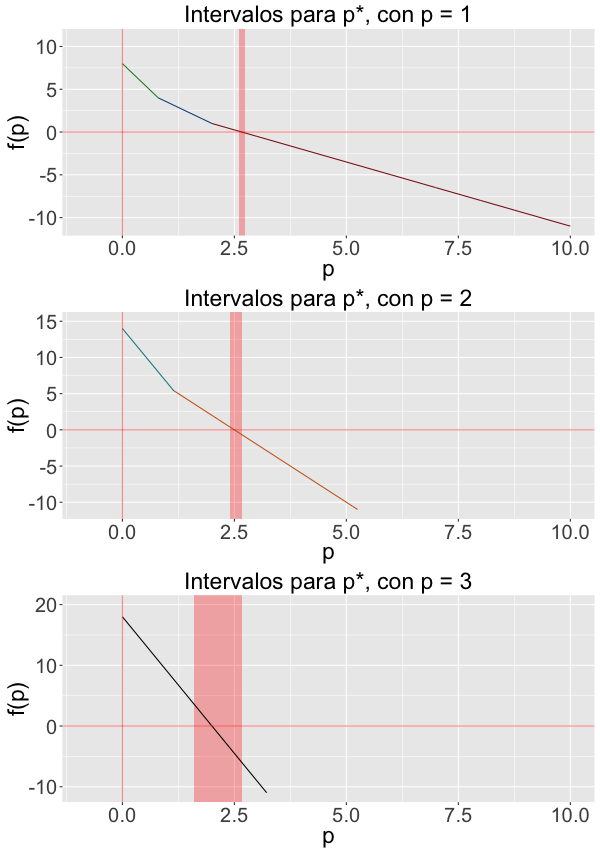
\includegraphics[width=.9\textwidth]{Figures/Chapter2_grid3eigen_interv}  
  \caption[Intervalos para $\rho^*$.] {La figura superior representa intervalos para $\rho^*$ cuando $f(\rho) = \lambda_{G(\rho)_1}$, la de enmedio cuando $f(\rho) = \lambda_{G(\rho)_1} + \lambda_{G(\rho)_2}$ y la de abajo cuando $f(\rho) = \lambda_{G(\rho)_1} + \lambda_{G(\rho)_2} + \lambda_{G(\rho)_3}$.}
\end{figure}

\end{example}

Otro intervalo que se ha desarrollado tiene que ver con directamente con los eigenvalores de $A$ y $B$ en lugar de los obtenidos por la matriz $A-\rho B$:

\pagebreak
\begin{proposition}
Sea $B$ positiva definida, entonces la raíz $\rho^*$ de $f(\rho)$ es tal que \cite{ngo2012trace}:

\begin{equation*}
\frac{\sum_{i = 1}^{p}\lambda_{A_i}}{\sum_{i = 1}^{p}\lambda_{B_i}} \leq \rho^* \leq \frac{\sum_{i = 1}^{p}\lambda_{(A)_i}}{\sum_{i = 1}^{p}\lambda_{(B)_{n-i+1}}}	
\end{equation*}

con $\lambda_{A_i}$ y $\lambda_{B_i}$ el i-ésimo eigenvalor más grande  de la matriz $A$ y $B$ respectivamente \cite{ngo2012trace}. 
\end{proposition}


\begin{proof}
Se tiene la propiedad que para una $p$ dada:


\begin{equation}\label{eq:2.44}
\max_{V^T V = I} Tr(V^T A V) =  Tr(V^{T*} A V^*) = \sum_{i=1}^p \lambda_{A_i }
\end{equation}
 
Con $\lambda_{A_i}$ los eigenvalores de A. Como esta $V^*$ maximiza la traza sobre $A$, entonces no necesariamente maximiza la de $B$. Al sustituirla en $Tr(V^{T} B V)$ se tiene que: 

\begin{equation}\label{eq:2.45}
Tr(V^{T*} B V^*) \leq \sum_{i=1}^p \lambda_{B_i }
\end{equation}

Con $\lambda_{B_i}$ los eigenvalores de B. Al hacer el cociente de (1.43) y (1.44) Se puede acotar inferiormente a $\rho^*$:


\begin{equation*}
  \frac{\sum_{i=1}^p \lambda_{A_i}} {\sum_{i=1}^p \lambda_{B_i}} \leq \frac{Tr(V^{T*} A V^*)}{Tr(V^{T*} B V^*)} \leq \max_{V^T V} \frac{Tr(V^{T} A V)}{Tr(V^{T} B V)} = \rho^*
\end{equation*}

Ahora falta acotarlo superiormente. Usando las siguientes propiedades que son derivadas de (1.27):

\begin{equation}\label{eq:2.46}
  Tr(V^T A V) \leq \sum_{i=1}^p \lambda_{A_i} 
\end{equation}

\begin{equation}\label{eq:2.47}
  Tr(V^T B V) \geq \sum_{i=1}^p \lambda_{B_{(n-i+1)}}
\end{equation}

La expresión (1.46) es la suma de los p eigenvalores más chicos de $B$. Dividiendo (1.45) entre (1.46) se tiene que para cualquier matriz ortogonal $V$:

\begin{equation}\label{eq:2.48}
   \frac{Tr(V^{T} A V)}{Tr(V^{T} B V)} \leq \frac{\sum_{i=1}^p \lambda_{A_i}}{\sum_{i=1}^p \lambda_{B_{(n-i+1)}}}
\end{equation}

En particular si se toma $V = V^{**}$ (La matriz con la que se alcanza $\rho^*)$:

\begin{equation}\label{eq:2.49}
  \rho^* = \frac{Tr(V^{T**} A V^{**})}{Tr(V^{T**} B V^{**})} \leq \frac{\sum_{i=1}^p \lambda_{A_i}}{\sum_{i=1}^p \lambda_{B_{(n-i+1)}}}
\end{equation}

\end{proof}
\begin{example}
Para ejemplificar esta cota se usará las matrices $A$ y $B$ de los dos ejemplos anteriores y se muestra en la figura 1.7.


\begin{equation*}
A = \left(\!
    \begin{array}{ccc}
      4 & 0 & 0 \\
      0 & 6 & 0 \\
      0 & 0 & 8 
    \end{array}
  \!\right), \quad
B = \left(\!
    \begin{array}{ccc}
      1.5 & 0 & 0 \\
      0 & 2.5 & 0 \\
      0 & 0 & 5 
    \end{array}
\!\right) 
\end{equation*}


(i) Para $p = 1$ la cota es la siguiente:
\begin{equation*}
\begin{aligned}
  \lambda_{A_1} = 8 \qquad
  \lambda_{B_1} = 5 \qquad
  \lambda_{B_3} = 1.5
\end{aligned}
\end{equation*}

\begin{equation*}
\begin{aligned}
\rho_1 = \frac{\sum_{i = 1}^{p}\lambda_{A_i}}{\sum_{i = 1}^{p}\lambda_{B_i}}  = \frac{8}{5} \qquad
\rho_2 = \frac{\sum_{i = 1}^{p}\lambda_{A_i}}{\sum_{i = 1}^{p}\lambda_{B_{n-i+1}}}  = \frac{8}{1.5}
\end{aligned}
\end{equation*}

(ii) Para $p = 2$ la cota es la siguiente:

\begin{equation*}
\begin{aligned}
\sum_{i = 1}^{2}\lambda_{A_1}  =& 14 \qquad
\sum_{i = 1}^{2}\lambda_{B_1}  =& 7.5 \qquad
\sum_{i = 1}^{2}\lambda_{B_{3-i+1}} =& 4
\end{aligned}
\end{equation*}

\begin{equation*}
\begin{aligned}
\rho_1 = \frac{\sum_{i = 1}^{p}\lambda_{A_i}}{\sum_{i = 1}^{p}\lambda_({B_i)}}
 = \frac{14}{7.5} \qquad
\rho_2 = \frac{\sum_{i = 1}^{p}\lambda_{A_i}}{\sum_{i = 1}^{p}\lambda_{B_{n-i+1}}}  = \frac{14}{4}
\end{aligned}
\end{equation*}



(iii) Para $p = 3$ la cota es la siguiente:
\begin{equation*}
  \begin{aligned}
  \sum_{i = 1}^{3}\lambda_{A_1}  = 18 \qquad
  \sum_{i = 1}^{3}\lambda_{B_1}  = 9 \qquad
  \sum_{i = 1}^{3}\lambda_{B_{n-i+1}}  = 9
  \end{aligned}
\end{equation*}

\begin{equation*}
  \begin{aligned}
\rho_1 = \frac{\sum_{i = 1}^{p}\lambda_{A_i}}{\sum_{i = 1}^{p}\lambda_{B_i}}  = \frac{18}{9} \qquad
\rho_2 = \frac{\sum_{i = 1}^{p}\lambda_{A_i}}{\sum_{i = 1}^{p}\lambda_{B_{n-i+1}}}  = \frac{18}{9}
  \end{aligned}
\end{equation*}

\end{example}

\begin{figure}[!ht] \label{Fig1.7}
  \centering
  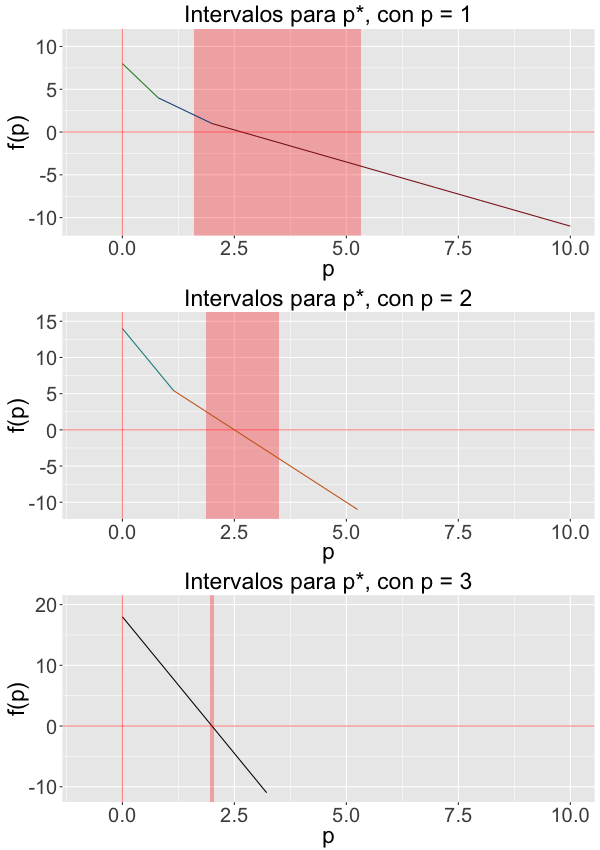
\includegraphics[width=.9 \textwidth]{Figures/Chapter2_grid3eigen_interv2}  
  \caption[Intervalos para $\rho^*$.] {La figura superior representa intervalos para $\rho^*$ cuando $f(\rho) = \lambda_{G(\rho)_1}$, la de enmedio cuando $f(\rho) = \lambda_{G(\rho)_1} + \lambda_{G(\rho)_2}$ y la de abajo cuando $f(\rho) = \lambda_{G(\rho)_1} + \lambda_{G(\rho)_2} + \lambda_{G(\rho)_3}$.}
\end{figure}




	\chapter{El Método Newton-Lanczos}
\label{ch:chapter3}
 
En el capítulo anterior se propuso una función no creciente $f(\rho)$ cuya raíz resulta ser la solución óptima para el problema del Discriminante Lineal de Fisher:

\begin{equation} \label{eq:3.1}
	f(\rho) = \max_{V^T V = I} Tr(V^T(S_E - \rho S_I)V)
\end{equation}

El algoritmo propuesto para encontrar la solución recibe el nombre de Newton-Lanczos\cite{ngo2012trace}. Para entenderlo a profundidad, se explicarán brevemente los métodos de Lanczos que tridiagonalizan una matriz simétrica, para después calcular eficientemente los primeros (últimos) eigenvalores. Después, será implementado junto al método iterativo de Newton, que calcula el nuevo valor de $\rho_{n}$ para cada paso. Para esto, se requiere el cómputo de la derivada de $f(\rho)$, por lo que se desarrollará su forma analítica. Finalizando, se proporcionarán las condiciones necesarias de optimalidad.

La primera división de los métodos para calcular eigenvectores y eigenvalores que propone J. Demmel \cite{demmel1997applied} depende si la matriz es simétrica o no lo es. Después hace una sub-clasificación dependiendo si el método es iterativo o directo. Para este texto solo se calcularán los eigenvalores de matrices simétricas, por lo que el procedimiento a seguir sera el siguiente:


\begin{itemize}
\item Tridiagonalizar la matriz simétrica por un método iterativo
\item Encontrar los eigenvalores por medio de la iteración tridiagonal QR (LAPACK DSTEVD)
\end{itemize}
\section{Métodos de Lanczos}
Antes de presentar los métodos de Lanczos, se dará una breve introducción acerca del costo computacional del algoritmo QR y la importancia de tridiagonalizar la matriz \cite{demmel1997applied}.  Sea $A \in {\rm I\!R}^{n \times n}$, entonces su descomposición $QR$ toma $O(n^3)$ flops. Suponiendo el mejor escenario en el que cada eigenvalor se encuentra con una iteración, tomaría $O(n^4)$ flops para calcular todos los eigenvalores de una matriz. Por otra parte, al tridiagonalizar la matriz $A$ se reduce el costo computacional de la descomposición $QR$ a $O(n^2)$ flops. De esta manera, tomaría $O(n^3)$ flops encontrar todos los eigenvalores. Una descripción más detallada del costo computacional de los algoritmos puede encontrarse en \cite{demmel1997applied}.

El primer paso, la tridiagonalización, ha sido muy estudiado y existen algoritmos especializados para distintos tipos de matrices simétricas. Si la matriz es de gran dimensión y rala, entonces se recomienda usar el método de Lanczos \cite{golub2012matrix}. En otro caso, existen las transformaciones Householder y las rotaciones de Givens \cite{golub2012matrix}. El método de Lanczos realiza tridiagonalizaciones parciales de la matriz original $A$, donde cada una es de tamaño $p \times p$ con $p\leq n$. Un aspecto interesante es que las matrices parciales van aproximando los eigenvectores extremos antes que la tridiagonalización esté completa. Por este motivo, el algoritmo es usado cuando se requieren solo algunos de los eigenvalores. Con respecto al costo computacional, es del orden $O(n^3)$, por lo que el algoritmo completo se mantiene en el mismo orden. 

Lanczos en aritmética exacta tiene muchas ventajas computacionales y converge rápidamente a los eigenvalores reales, pero con aritmética inexacta es difícil usarlo en la práctica \cite{golub2012matrix}. El problema que se presenta es que los eigenvectores van perdiendo la ortogonalidad entre ellos conforme la dimensionalidad y las iteraciones incrementan. Los textos \cite{demmel1997applied}\cite{golub2012matrix} incluyen algoritmos para solucionar este problema.

En la siguiente subsección se presentará el algoritmo original de Lanczos; se ejemplificará como los eigenvalores de la matriz tridiagonal convergen a los originales y se presenta el problema de \textit{ghost eigenvalues} \cite{demmel1997applied}, que son los eigenvalores que surgen al perder la ortogonalidad en aritmética inexacta.

\subsection{Algoritmo de Lanczos}

El algoritmo de Lanczos busca calcular los elementos de esta matriz tridiagonal directamente. Definiendo $Q^T A Q = T$, con $Q = [q_{(1)} \enskip|\enskip q_{(2)} \enskip|\enskip ... \enskip|\enskip q_{(n)}]$ ortogonal, y $T_n$ tridiagonal igual a:

\begin{equation}\label{eq:3.2}
T_n = \left(\!
    \begin{array}{cccccc}
      \alpha_1 & \beta_2 &  &  &  & 0\\
      \beta_2  & \alpha_2 & \beta_3 &  &  & \\
               & \beta_3 & \alpha_3 &  \ddots  & & \\
               &         & \ddots & \ddots & \beta_{n-1}& \\
               &  &  &  \beta_{n-1} & \alpha_{n-1} & \beta_n\\
       0       &  &  &  & \beta_n & \alpha_{n}\\
    \end{array}
  \!\right), \quad
\end{equation}

Como $q_{(1)}$ es una columna de Q, entonces $q_1^T = [q_{11},\enskip q_{21},\enskip ... ,\enskip q_{n1}]$. De esta manera, se tiene que $AQ = QT$. Descomponiendo la multiplicación $AQ =[Aq_{(1)} \enskip|\enskip Aq_{(2)} \enskip|\enskip ... \enskip|\enskip Aq_{(n)}]$ e igualándola a cada columna de $QT$, se tiene que $Aq_{(1)}$ \cite{golub2012matrix}:

\begin{equation*}
\begin{aligned}
Aq_{(1)} =\quad &  q_{(1)(1)} \alpha_{(1)}       &+\quad q_{(1)(2)} \beta_{(2)} \quad&+ \\
     & q_{(2)(1)}   \alpha_{(1)}       &+\quad q_{(2)(2)} \beta_{(2)} \quad&+ \\
     &          \qquad         \vdots&\vdots \qquad     & \\
     & q_{(n)(1)}   \alpha_{(1)}       &+\quad q_{(n)(2)} \beta_{(2)} \quad& \\
Aq_{(1)} =\quad & \alpha_{(1)} q_{(1)} &+\quad \beta_{(2)} q_{(2)}   \qquad& 
\end{aligned}
\end{equation*}

Ahora, para $i = 2, ..., n-1$
  
\begin{equation*}
\begin{aligned}
Aq_{(i)} =\quad &  q_{(i-1)(i-1)}\beta_{(i)}  &+ \enskip q_{(i-1)(i)}\alpha_{(i)} &+ \enskip q_{(i-1)(i+1)} \beta_{(i+1)} &+ \\
     & q_{(i)(i-1)}\beta_{(i)}       &+ \enskip q_{(i)(i)}\alpha_{(i)}\enskip   &+\enskip q_{(i)(i+1)} \beta_{(i+1)}   &+ \\
     & \vdots &          \qquad \qquad \quad \vdots & &\\
     & q_{(n)(i-1)}\beta_{(i)}      &+\enskip q_{(n)(i)}\alpha_{(i)} \enskip  &+\enskip q_{(n)(i+1)} \beta_{(i+1)}   & \\
Aq_{(i)} =\quad & \beta_{(i)} q_{(i-1)}      &+ \enskip\quad \alpha_{(i)} q_{(i)} \quad    &+\enskip \beta_{(i+1)} q_{(i+1)}      &
\end{aligned}
\end{equation*}

Por último, para $Aq_n$:

\begin{equation*}
\begin{aligned}
Aq_{(n)} =\quad &  q_{(1)(n)} \alpha_{(n)}       &+\quad q_{(1)(n-1)} \beta_{(n)} \quad&+ \\
     & q_{(2)(n)}   \alpha_{(n)}       &+\quad q_{(2)(n-1)} \beta_{(n)} \quad&+ \\
     &          \qquad         \vdots&\vdots \qquad     & \\
     & q_{(n)(n)}   \alpha_{(n)}       &+\quad q_{(n)(n-1)} \beta_{(n)} \quad& \\
Aq_{(n)} =\quad & \alpha_{(n)} q_{(n)} &+\quad \beta_{(n)} q_{(n-1)}   \qquad& 
\end{aligned}
\end{equation*}


Si se define $q_{(0)} = 0$, entonces se puede resumir el paso como:

\begin{equation}\label{eq:3.3}
  Aq_{(i)} = \beta_{(i)} q_{(i-1)} + \alpha_{(i)} q_{(i)}+ \beta_{(i+1)} q_{(i+1)}
\end{equation}

para $i = 1, .... n-1$. Multiplicando esta expresión por $q_{(i)}^T$, y usando el supuesto de ortogonalidad, entonces $q_{(i)}^T q_{(j)} = 0$ con $i \neq j$. De esta manera resulta la siguiente expresión:

\begin{equation}\label{eq:3.4}
\begin{aligned}
  q_{(i)}^TAq_{(i)} &=  q_{(i)}^T\alpha_{(i)} q_{(i)}  
                    &= \alpha_{(i)}
\end{aligned}
\end{equation}

Por otra parte, despejando $\beta_{(i+1)} q_{(i+1)}$ de \ref{eq:3.3}, se tiene que

\begin{equation}\label{eq:3.5}
\begin{aligned}
\beta_{(i+1)} q_{(i+1)}  =& Aq_{(i)} - \beta_{(i)} q_{(i-1)} - \alpha_{(i)} q_{(i)} \\ 
=& (A - \alpha_{(i)} I) q_{(i)} - \beta_{(i)} q_{(i-1)} = r_{(i)}
\end{aligned}
\end{equation}

Con la ecuación \ref{eq:3.5}, $q_{(i+1)} = \frac{r_{(i)}}{\beta_{(i+1)}}$. Calculando la norma de $r_{(i)}$, se tiene que 

\begin{equation}\label{eq:3.6}
\begin{aligned}
||r_{(i)}||_2 =& |\beta_{(i+1)}| ||q_{(i+1)}||_2 \\
              =& |\beta_{(i+1)}|
\end{aligned}
\end{equation}
 
Cuando $r_k =0$ entonces la iteración se detiene. \cite{golub2012matrix}

\pagebreak

\textbf{Implementación en aritmética exacta}\\

Sea $ A \in {\rm I\!R}^{n \times n}$ una matriz simétrica y $q_i \in {\rm I\!R}^{n}$. Entonces el algoritmo que se presenta a continuación produce una matriz $T_k \in {\rm I\!R}^{k \times k}$ tridiagonal tal que los eigenvalores de $T_k$ convergen a los de la matriz original $A$ \cite{golub2012matrix}. 

\begin{algorithm}[H] 
 $q_0$ $\leftarrow$ $0$\;
 $r_0$ $\leftarrow$ vector aleatorio\;
 $\beta_1$ $\leftarrow$ $||r_0||_2$\;
 $q_1 \leftarrow r_0 / \beta_1$\;
 $\alpha_1 \leftarrow q_1^T A q_1$\;
 $eps = 0.0000001$\;
 $k = 1$ \;
 \While{($\beta_k > eps$)}{
  $r_k \leftarrow A q_k - \alpha_k q_k - \beta_k q_{k-1}$\;
  $\beta_{k+1} \leftarrow ||r_{k-1}||_2$\;
  $q_{k+1} \leftarrow r_{k+1}/\beta{k+1}$\;
  $\alpha_{k+1} \leftarrow q_{k+1}^T A q_{k+1}$\;
  $k \leftarrow k+1$\;
 }
 \caption{Algoritmo de Lanczos}
\end{algorithm}

Para hacer frente a la pérdida de ortogonalidad entre los vectores, se han creado distintos métodos, los cuales se basan en la reortogonalización de la base de vectores. \cite{demmel1997applied} Esta puede realizarse en $O(n^2)$ operaciones, por lo que no afecta el orden de $O(n^3)$ flops.

\section{Derivada de $f(\rho)$}

La fórmula analítica de la derivada de $f(\rho)$ se puede obtener con cálculo multivariado. Para encontrarla, sea $V(\rho) \in {\rm I\!R}^{n \times p}$ una función diferenciable con respecto a $\rho$. Esta cumple la característica de ser una matriz ortogonal con columnas:

\begin{equation*}
	V(\rho) = (v_1(\rho) \enskip|\enskip v_2(\rho) \enskip|\enskip ... \enskip|\enskip v_p(\rho))
\end{equation*}

Antes de calcular la derivada de $f(\rho)$, es conveniente examinar la derivada de $V(\rho)^T V(\rho)$ con respecto a $\rho$. Sea $V(\rho)$ una matriz ortogonal; es decir, que cumpla $V^T(\rho) V(\rho) = I$, entonces \cite{ngo2012trace}:

\begin{equation*}
\frac{d}{d\rho} V(\rho)^T V(\rho) = \left(\frac{d}{d\rho}V(\rho)^T\right) V(\rho)  + V(\rho)^T 	\left( \frac{d}{d\rho} V(\rho) \right)
\end{equation*}

\vspace{5mm}

La derivada de $V(\rho)$ no se conoce explícitamente, pero se puede derivar componente a componente. De esta manera:


\begin{equation*}
\begin{aligned}
V(\rho)^T V(\rho)  &= \left(\!
    \begin{array}{cccc}
      v_{11}(\rho) & v_{21}(\rho) & \hdots & v_{n1}(\rho) \\
      v_{12}(\rho) & v_{22}(\rho) & \hdots & v_{n2}(\rho) \\
      \vdots & \vdots & \vdots & \vdots \\
      v_{1p}(\rho) & v_{2p}(\rho) & \hdots & v_{np}(\rho) 
    \end{array}
  \!\right)
    \left(\!
    \begin{array}{cccc}
      v_{11}(\rho) & v_{12}(\rho) & \hdots & v_{1p}(\rho) \\
      v_{21}(\rho) & v_{22}(\rho) & \hdots & v_{2p}(\rho) \\
      \vdots & \vdots & \vdots & \vdots \\
      v_{n1}(\rho) & v_{n2}(\rho) & \hdots & v_{np}(\rho) 
    \end{array} 
    \!\right) \\
    \vspace{5mm}
 &= \left(\!
    \begin{array}{c}
      v_{1}(\rho)^T \\
      v_{2}(\rho)^T \\
      \vdots \\
      v_{p}(\rho)^T  
    \end{array}
  \!\right)
  \left(\!
    \begin{array}{cccc}
      v_{1}(\rho) & v_{2}(\rho) & \hdots & v_{p}(\rho) 
    \end{array} 
	\!\right) 
\end{aligned}
\end{equation*}

Entonces la entrada $(i,j)$ de $V(\rho)^T V(\rho)$ es:

\begin{equation*}
	[V(\rho)^T V(\rho)]_{ij} = v_i(\rho)^T v_j(\rho)
\end{equation*}

Calculando la derivada:

\begin{equation*}
\frac{d}{d\rho}[V(\rho)^T V(\rho)]_{ij} =  \left( \frac{d}{d\rho}v_i(\rho)^T \right)  v_j(\rho) + v_i(\rho)^T \left( \frac{d}{d\rho} v_j(\rho)\right) 
\end{equation*}

En específico para el caso $i = j$:
\vspace{5mm}
\begin{equation}\label{eq:3.7}
\frac{d}{d\rho}[V(\rho)^T V(\rho)]_{ii} =  2 \left( \frac{d}{d\rho}v_i(\rho)^T \right)  v_i(\rho)
\end{equation}

\bigskip

\begin{lemma}\label{lemma:3.1}
Sea $V(\rho) \in {\rm I\!R}^{n \times p}$ una matriz ortogonal y $\rho$ su parámetro. Entonces \cite{ngo2012trace}:
\begin{equation*}
\begin{aligned}
(i)&  \quad \frac{d}{d\rho} V(\rho)^TV(\rho) = \left(\frac{d}{d\rho}V(\rho)^T\right) V(\rho)  + V(\rho)^T  \left( \frac{d}{d\rho} V(\rho) \right) = 0 \\
(ii)& \quad Diag \left(\left(\frac{d}{d\rho}V^T \right)V(\rho) \right) = 0 
\end{aligned}
\end{equation*}
\end{lemma}

\begin{proof}
\bigskip
(i) Para demostrar la primer propiedad se hace uso de que $V(\rho)^T V(\rho) = I_p$, entonces:
\begin{equation*}
\frac{d}{d\rho} [V(\rho)^T V(\rho)] = 0  
\end{equation*}

(ii) Se parte de la ecuación (\ref{eq:3.7}), y se usa el punto (i):
\begin{equation*}
  \frac{d}{d\rho} [V(\rho)^T V(\rho)]_{ii} =    2 \left( \frac{d}{d\rho}v_i(\rho)^T \right)  v_i(\rho) = 0
\end{equation*}

Como cada elemento $i$ es cero, entonces en particular $Diag\left( \left(\frac{d}{d\rho}V(\rho)^T \right) V(\rho) \right)=0 $.
\end{proof}

Del lema \ref{lemma:3.1} se tiene que $\left(\frac{d}{d\rho}V(\rho)^T \right) V(\rho)$ tiene diagonal igual a 0. Ahora, para derivar $f(\rho)$, primero se deriva la expresión $\frac{d}{d\rho}\left[V^T (A-\rho B)V \right]$:

\begin{equation}\label{eq:3.8}
\begin{aligned}
	\frac{d}{d\rho}\left[V^T (A-\rho B)V \right] & = \frac{d}{d\rho} \left[V^T A V \right]- \frac{d}{d\rho}\left[V^T \rho B V\right] \\
	& = \frac{dV^T}{d\rho}  AV +  V^T A \frac{dV}{d\rho} - \frac{dV^T}{d\rho} \rho BV - V^T \left[BV + \rho B \left(\frac{dV}{d\rho} \right) \right] \\
	& = \frac{dV^T}{d\rho} \left[A -\rho B \right] V + V^T \left[A- \rho B \right]\frac{dV}{d\rho} - V^TBV \\
\end{aligned} 
\end{equation}


Sea $V$ la matriz que diagonaliza $(A-\rho B)$, de manera que $V^T (A-\rho B) V = D$. Entonces \ref{eq:3.8}:
\begin{equation}\label{eq:3.9}
\begin{aligned}
\frac{d}{d\rho}\left[V^T (A-\rho B)V \right] & = \frac{dV^T}{d\rho} VD  + DV^T\frac{dV}{d\rho} - V^TBV 
\end{aligned}
\end{equation}

Al calcular la traza de (\ref{eq:3.9}) y usando del lema \ref{lemma:3.1}, se tiene que:
\begin{equation}\label{eq:3.10}
\begin{aligned}
Tr\left[\frac{d}{d\rho} \left[V^T (A-\rho B)V \right]\right] & = Tr\left[ \frac{dV^T}{d\rho} VD + DV^T \frac{dV}{d\rho} - V^T B V  \right] \\
											     & = 2 Tr \left[ D V^T \frac{dV}{d\rho} \right] - Tr \left[ V^T B V \right] \\
											     & = -Tr\left[V^T B V \right] 
\end{aligned}	
\end{equation}

\section{Método Newton-Lanczos}

El método de Newton establece que la iteración está dada por:

\begin{equation*}
x_{(n+1)} = x_{(n)} - \frac{f(x_n)}{f'(x_n)}
\end{equation*}

con $f'(x_n)$ la derivada de $f(x_n)$.

Con esta fórmula y con (\ref{eq:3.10}), se puede calcular explícitamente $\rho_{n+1}$ para la iteración de Lanczos \cite{ngo2012trace}:

\begin{equation}\label{eq:3.11}
\begin{aligned}
\rho_{n+1} =& \rho_{n} - \frac{Tr\left[V^T (A-\rho_n B)V \right]}{-Tr\left[V^T B V \right]} \\ \\
           =& \frac{\rho_{n} Tr\left[V^T B V \right] +  Tr\left[V^T (A-\rho_n B)V \right]}{Tr\left[V^T B V \right]}\\ \\
           =& \frac{\rho_{n} Tr\left[V^T B V \right] +  Tr\left[V^T A V \right] - \rho_nTr\left[V^T BV \right]}{Tr\left[V^T B V \right]} \\ \\
           =&\frac{Tr\left[V^T A V \right]}{Tr\left[V^T B V \right]}
\end{aligned} 
\end{equation}

Una vez calculado el paso de la iteración, se enuncia el método de Newton-Lanczos para maximizar el cociente de trazas. El método recibe como entrada la matriz $A$, $B$ y la dimensión a la cual se desea proyectar $p$ \cite{ngo2012trace}: 

\begin{algorithm}[H]
i = 1\;
$\rho_1$ un número aleatorio\;
$\rho_0$\;
$f(\rho_1) = \sum\limits_{j = 1}^{p} \lambda_{(A-\rho_1 B)_j}$\;
V = primeros $p$ eigenvectores de $A-\rho_1 B$\;
$tol = 1e-10$\;

\While{($i<50$ \quad , \quad $abs(\rho_i-\rho_{i-1}$)$>tol$)}{
$i = i+1$\;
V = primeros $p$ eigenvectores de $(A-\rho_i B)$ \;
$\rho_i = Tr(V^T A V)/Tr(V^T BV)$\;
$f(\rho_i) = \sum\limits_{j = 1}^{p} \lambda_{(A-\rho_i B)_j}$\;
}
 \caption{Algoritmo de Newton-Lanczos}
\end{algorithm}


\subsection{Condiciones necesarias de optimalidad}
Considerando el problema de maximizar las trazas:

\begin{equation}\label{eq:3.12}
  \max_{\substack{V \in {\rm I\!R}^{n \times p} \\ V^TV = I}} \frac{Tr(V^T S_E V)}{Tr(V^T S_I V)} 
\end{equation}

La función lagrangiana asociada a este problema es la siguiente \cite{ngo2012trace}:

\begin{equation*}
L(V, \Gamma) =  \frac{Tr(V^T S_E V)}{Tr(V^T S_I V)} - Tr[\Gamma(V^TV-I)]
\end{equation*}

Con $\Gamma \in {\rm I\!R}^{p \times p}$ , la matriz de multiplicadores de Lagrange de la forma:

\begin{equation*}
\Gamma = \left(\!
    \begin{array}{ccccc}
    \gamma_{(1)(1)} & \gamma_{(1)(2)} & \hdots & \gamma_{(1)(p-1)} & \gamma_{(1)(p)} \\
    \gamma_{(2)(1)} & \gamma_{(2)(2)} & \hdots & \gamma_{(2)(p-1)} & \gamma_{(2)(p)} \\
    \vdots & \vdots & \vdots & \vdots & \vdots \\
    \gamma_{(p-1)(1)} & \gamma_{(p-1)(2)} & \hdots & \gamma_{(p-1)(p-1)} & \gamma_{(p-1)(p)} \\
    \gamma_{(p)(1)} & \gamma_{(p)(2)} & \hdots & \gamma_{(p)(p-1)} & \gamma_{(p)(p)} \\
\end{array}
  \!\right), \quad
\end{equation*}


Ya que al multiplicar esta matriz por $[V^T V- I]$ (con $V = (v_1 \enskip |\enskip v_2 \enskip |\enskip ... \enskip |\enskip v_{p-1} \enskip |\enskip v_p)$) se tiene que: 

\begin{equation*}
V^T V - I = \left(\!
    \begin{array}{ccccc}
    v_1^T v_1 -1& v_1^T v_2 & \hdots & v_1^T v_{p-1} & v_1^T v_p \\
    v_2^T v_1 & v_2^T v_2 -1& \hdots & v_2^T v_{p-1} & v_2^T v_p \\
    \vdots & \vdots & \vdots & \vdots & \vdots \\
    v_{p-1}^T v_1 & v_{p-1}^T v_2 & \hdots & v_{p-1}^T v_{p-1} -1& v_{p-1}^Tv_p \\
    v_p^T v_1 & v_p^T v_2 & \hdots & v_p^Tv_{p-1} & v_{p}^Tv_{p} -1 \\
\end{array}
  \!\right), \quad
\end{equation*}

entonces, la diagonal de ($\Gamma (V^T V - I)$) contiene $p$ elementos que son los siguientes: 

\begin{equation*}
\left(\!
    \begin{array}{c}
    \begin{aligned}
    & \gamma_{(1)(1)}(v_1^T v_1 -1) &+& \gamma_{(1)(2)} (v_2^T v_1) &+& \hdots &+& \gamma_{(1)(p)}(v_p^T v_1) &\\
    & \gamma_{(2)(1)}(v_1^T v_2) &+& \gamma_{(2)(2)}(v_2^T v_2 -1)  &+& \hdots &+& \gamma_{(2)(p)}(v_p^T v_2) &\\
    & \vdots && \vdots && \vdots && \vdots &\\
    &\gamma_{(p-1)(1)}(v_1^T v_{p-1}) &+& \gamma_{(p-1)(2)} (v_2^T v_{p-1}) &+& \hdots &+& \gamma_{(p-1)(p)}(v_p^T v_{p-1})&\\
    &\gamma_{(p)(1)}(v_1^T v_{p}) &+& \gamma_{(p)(2)}(v_2^T v_p)  &+& \hdots &+& \gamma_{(p)(p)}(v_p^T v_{p}-1) &\\
\end{aligned}
\end{array}
  \!\right), \quad
\end{equation*}

Para calcular la traza se suman estos elementos de la diagonal. De esta forma, se tienen p restricciones de la forma $v_i^T v_i = 1 \quad i = 1,...,p$ y $p(p-1)$ restricciones de la 
forma $v_i^T v_j = 0 \quad i \neq j, \quad i,j = 1, ..., p$, cada una con su multiplicador lagrangiano.

Como la ecuación a maximizar tiene un maximizador global $V^*$, entonces existe un multiplicador matricial lagrangiano tal que en el óptimo:

\begin{equation}\label{eq:3.13}
\frac{\partial \mathcal{L}(V^*, \Gamma^*)}{\partial V} =  0 \qquad con \qquad V^{T*}V^* = I
\end{equation}

Para encontrar $(V^*, \Gamma^*)$ de (\ref{eq:3.13}), primero se debe conocer la derivada de $\frac{\partial Tr(V^T M V)}{\partial V}$, con M cualquier matriz:

\begin{equation}\label{eq:3.14}
\frac{\partial Tr(V^T M V)}{\partial V} = (M^* +M)V  
\end{equation}

\pagebreak
Derivando el lagrangiano (\ref{eq:3.13}) y utilizando (\ref{eq:3.14}) se tiene que:

\begin{equation*}
\begin{aligned}
\frac{\partial \mathcal{L}(V, \Gamma)}{\partial V} =&\quad  \left[\frac{\partial Tr(V^T A V) }{\partial V}\right]\left[Tr(V^T B V)^{-1}\right] \quad +& \\
&\quad \left[Tr(V^T A V)\right]\left[\frac{\partial (Tr(V^T B V))^{-1} }{\partial V}\right] \quad -& \\
&\quad \left[\frac{\partial Tr[\Gamma(V^TV-I)] }{\partial V}\right] \quad &
\end{aligned}
\end{equation*}
\vspace{5mm}

\begin{equation*}
\begin{aligned}
\frac{\partial \mathcal{L}(V, \Gamma)}{\partial V} =&\quad  \left[2AV\right]\left[Tr(V^T B V)^{-1}\right] \quad +& \\
&\quad \left[Tr(V^T A V)\right]\left[\frac{2BV}{Tr(V^T B V)^2}\right] \quad -& \\
&\quad \left[V (\Gamma^* + \Gamma) \right] \quad &
\end{aligned}
\end{equation*}
\vspace{5mm}

\begin{equation}\label{eq:3.15}
\begin{aligned}
\frac{\partial \mathcal{L}(V, \Gamma)}{\partial V} =&\quad  \left[\frac{2AV Tr(V^T B V)- 2BV Tr(V^T A V)}{(Tr(V^T B V))^2}\right] \quad +& \\
&\quad \left[V (\Gamma^* + \Gamma) \right] \quad &
\end{aligned}
\end{equation}

Igualando (\ref{eq:3.15}) a cero y acomodando la expresión, resulta:
\begin{equation*}
\left[A-\frac{Tr(V^{T*} A V^*)}{Tr(V^{T*} B V^*)}B\right] V^*  = \left[\frac{Tr(V^{T*} B V^*)}{2}V^* (\Gamma^{T*} + \Gamma^{*})\right]
\end{equation*}

\begin{equation}\label{eq:3.16}
\left[ A-\rho^* B\right]V^*   = \left[ \frac{Tr(V^{T*} B V^*)}{2}V^* (\Gamma^{T*} + \Gamma^{*}) \right]
\end{equation}

Con $\rho^* = \frac{Tr(V^{T*} A V^*)}{Tr(V^{T*} B V^*)}$. Sea $Q$ la matriz ortogonal que diagonaliza $\Gamma^{T*} + \Gamma^{*}$, entonces se puede escribir la expresión $(\Gamma^{T*} + \Gamma^*)$ como:
\begin{equation*}
 \left(\Gamma^{T*} + \Gamma^{*}\right) = Q \Sigma^* Q^T \qquad con \qquad Q^TQ = I
\end{equation*}

Con $\Sigma^*$ una matriz diagonal. Multiplicando (\ref{eq:3.16}) por $V^{T*}$ y calculando la traza de ambos lados de la ecuación y se tiene que:

\begin{equation*}
\begin{aligned}
Tr\left[ V^{T*}(A-\rho^* B)V^*\right]  =& \left[ \frac{Tr(V^{T*} B V^*)}{2}\right] Tr(\Gamma^{T*} + \Gamma^{*}) \\ \\
Tr(\Gamma^{T*} + \Gamma^{*}) =& 2 \frac{Tr(V^{T*}(A-\rho^*B)V^*)}{Tr(V^{T*}BV^*)} = 0 
\end{aligned}
\end{equation*}
\vspace{5mm}
\begin{equation}\label{eq:3.17}
Tr(Q \Sigma^* Q^T) = 2 \frac{Tr(V^{T*}(A-\rho^*B)V^*)}{Tr(V^{T*}BV^*)} = 0
\end{equation}


Como $Tr(V^{T*}(A-\rho^*B)V^*) = 0$ entonces $Tr(Q \Sigma^* Q^T) =0$, por lo que $Tr(\Sigma^*) = 0$. Definiendo $U^* = V^*Q$, con $U^*U = I$, la expresión (\ref{eq:3.16}) se puede escribir como:

\begin{equation*}
\begin{aligned}
\left[ A-\rho^* B\right]V^*   &= \left[ \frac{Tr(V^{T*} B V^*)}{2}V^* (Q \Sigma^* Q^T) \right] \\\\
                              &= \left[ \frac{Tr(V^{T*} B V^*)}{2}U^*Q^{T*} (Q \Sigma^* Q^T) Q \right] \\\\
                              &= \left[ \frac{Tr(V^{T*} B V^*)}{2}U^* \Sigma^* \right] \\
\end{aligned}
\end{equation*}  

Definiendo $\Lambda_* = \frac{Tr(V^{T*} B V^*)}{2}\Sigma^*$, entonces:
\begin{equation}\label{eq:3.18}
\begin{aligned}
\left[ A-\rho^* B\right]U^*   &= U^* \Lambda_* \\
 U^{T*} \left(A-\rho^* B\right)U^*   &=  \Lambda_* \\
 Tr(U^{T*} \left(A-\rho^* B\right)U^*)   &=  Tr(\Lambda_*) = 0
\end{aligned}
\end{equation}  

De esta manera se tiene que la ecuación (\ref{eq:3.18}) es la condición necesaria para que $U^*, \rho^*$ sean las óptimas










	\chapter{Experimentos numéricos}
\label{ch:chapter4}

Para medir el desempeño del algoritmo Newton-Lanczos se compara con otros dos métodos, el Análisis Discriminante Lineal (ADL) y la Regresión Logística Multinomial (RLM). Los criterios para elegir el mejor serán la tasa de reconocimiento y el tiempo de cómputo sobre los conjuntos de datos JAFFE y MNIST. Como el algoritmo de Newton-Lanczos ocupa los eigenvectores de una matriz, en la primer parte de este capítulo se medirá el tiempo de Lanczos y el costo de la rutina $SVD$ de R para una matriz en particular \footnote{La rutina $svd$ de $R$ ocupa la función $gesdd$ de la librería $LAPACK$. Para más información puede consultarse la página $http://www.netlib.org/lapack/$.}. En la segunda parte del capítulo, se explicará el preprocesamiento de las bases de datos y como se crearon los conjuntos de entrenamiento y prueba. En la tercer y cuarta parte, se realizan los experimentos con la bases de MNIST y JAFFE respectivamente. 

Para todos los experimentos de este capítulo, se utilizó el lenguaje de \textsf{R} en su versión 3.2.2 \textit{Fire Safety}. Los cálculos fueron realizados en una iMac 3.2 Ghz Intel Core i3 con 12 GB de RAM.

\section{Desempeño del método de Lanczos}

Antes de analizar el tiempo de cómputo de Newton-Lanczos, se evaluará el desempeño del algoritmo de Lanczos comparándolo con la factorización $svd$. Esto experimento es para saber en que casos es conveniente utilizar Lanczos y en cuales conviene calcular todos eigenpares. Para la prueba se usó $A - \rho B$ con $A$ y $B$ las matrices de dispersión intra clase y entre clase de la base de datos MNIST y con $\rho = 3$. La figura \ref{fig5.1} resume el desempeño de ambos métodos.

\begin{figure}[!ht] \label{fig5.1}
  \centering
  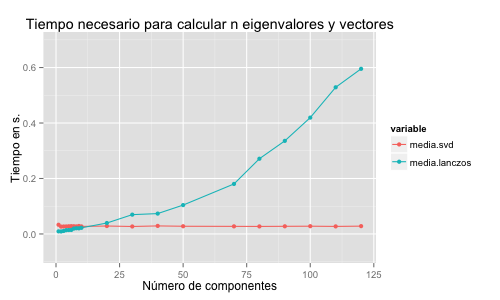
\includegraphics[width=1\textwidth]{Figures/Chapter4_eigen_lanczos.png} 
  \caption[Desempeño de Lanczos.] {Desempeño de Lanczos. En el eje $x$ se representa k, el número de eigenpares a calcular de la matriz $A- \rho B$. La matriz original es de 193 x 193. El tiempo reportado para cada $k$, es el promedio de $30$ repeticiones para cada método.}
\end{figure}

Se observa que, para $k$ menor a 10, el algoritmo de Lanczos es más rápido que la factorización $SVD$ de la matriz completa. Para valores más grandes, conviene factorizar toda la matriz. Esto puede deberse a que en aritmética inexacta Lanczos presenta el problema de \textit{Ghost eigenvalues} (eigenvalores que se repiten, pero que son espurios) \cite{golub2012matrix}. Estos se originan porque la ortogonalidad entre los eigenvectores se pierde conforme la dimensionalidad aumenta. Para solucionar este problema, se tuvo que realizar una reortogonalización completa en cada iteración, lo que pudo aumentar el tiempo de cómputo. 

\section{Modelos comparados y preprocesamiento de las bases}

En este capítulo, el método de Newton-Lanczos se comparó otros dos métodos de clasificación: la RLM y con el ADL. Para el primero, se usó la función \textit{multinom} del paquete \textit{nnet}, mientras que para el segundo se utilizó una modificación de la función \textit{lda} \footnote{La modificación está presentada en los códigos del apéndice B} del paquete \textit{MASS}. Ambas funciones fueron desarrolladas por Brian Ripley, profesor de estadística aplicada de la Universidad de Oxford. 

Como primer paso, se definieron los tamaños del conjunto de entrenamiento y prueba. Para el entrenamiento de MNIST se ocuparon 4000 datos (400 por clase); es decir, el 6\% del total. En el caso de JAFFE se utilizaron 50 datos (5 por clase); es decir, el 23\% del total. En ambos, el resto de los datos se ocupó en el conjunto de prueba. 

Para el preprocesamiento de las bases, cada imagen se convirtió en un vector con tamaño asociado al número de píxeles. Esto genera un problema de dimensionalidad, por lo que se realizó un paso de reducción dimensional. Se tomaron las primeras componentes principales (PCA) del conjunto de entrenamiento de manera que se explicara el 95\% de la varianza total, después se proyectó el conjunto de prueba. (De esta manera, los individuos en lugar de pertenecer a un espacio de ${\rm I\!R}^{m \times n}$, pertenecen a uno menor). Para MNIST se tomaron 193 de las 784 componentes; en cambio, para JAFFE solo 50 de las 65536. 

Una vez hecho el preprocesamiento, se realizaron 2 experimentos para cada base de datos. En el primero se utilizó el método de Newton-Lanczos con $V \in {\rm I\!R}^{m \times 20}$. Después de esto se proyectaron a los individuos originales a un espacio 20-dimensional. Los objetivos fueron los siguientes: 

\begin{itemize}
\item Analizar como cambia el valor de $f(\rho)$ con el método de Newton-Lanczos
\item Ver como se ven proyectados los datos en dimensiones menores
\end{itemize}

En el segundo experimento se entrenaron los 3 métodos con distintas $p$. Después se midió la tasa de reconocimiento alcanzada (usando el conjunto de prueba) y su tiempo de ejecución. 

\section{Base de datos MNIST}

Las siglas MNIST provienen de (\textit{Mixed National Institute of Standards and Technology}), la cual contiene datos de 70,000 dígitos escritos a mano que se usan comúnmente para probar códigos de clasificación de imágenes. De esta manera, en el experimento se tendrán 10 clases: los dígitos del 0-10. La base de datos surge de la colaboración de Yann LeCun del Instituto Courant (NYU), de Corinna Cortes de Google Labs (NY) y de Christopher J.C. Burges de Microsoft Research en Redmond. Puede descargarse de la página Web \textit{yann.lecun.com/exdb/mnist}, cuyo link sigue vigente al 13 de marzo del 2016.

Las imágenes están en un formato especial llamado IDX. Para poderlas convertir en un archivo leíble para R, se utilizó la función \textit{readMNIST} del paquete \textit{darch}. Esta paquetería convierte los archivos a objetos \textit{.RData}. La figura 3.2 contiene una extracto de tamaño 225 de todo el conjunto.

\begin{figure}[!ht]\label{fig5.2}
  \centering
	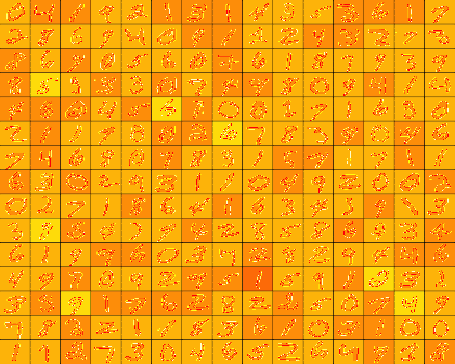
\includegraphics[width=1\textwidth]{Figures/Chapter4_numeros.png}	
  \caption{Ejemplo de números de la base de datos (MNIST).}
\end{figure}

\subsection{Proyección sobre un espacio de dimensión 20}

\underline{\textbf{1) Cotas para $\rho^*$}}

En el capítulo 2 se presentaron cotas para $\rho^*$ y en esta sección se ejemplificará la segunda de ellas para esta base de datos. Se calcularon los eigenvalores de la matriz intraclase (B) y de la matriz entre clases (A). Los 20 eigenvalores más grandes y más pequeños de la primera son \footnote{los eigenvalores menores a $1e^{-10}$ se consideraron numéricamente como 0}:

\begin{center}
\begin{tabular}{ | c | c|  c |c | c|  c |c | c|  c |c | c | c|  c |c | c|  c |c | c|  c |c |} 
\hline
12694 & 10367 & 7822 & 6793 & 6013 & 5887 & 5269 & 4704 & 4474 & 3969 \\
3833 & 3428 & 3124 & 3015 & 2978 & 2627 & 2535 & 2353 & 2232 & 2150 \\
\hline
\hline
\end{tabular}
\end{center}

\begin{center}
\begin{tabular}{ | c | c|  c |c | c|  c |c | c|  c |c | c | c|  c |c | c|  c |c | c|  c |c |} 
\hline
73 & 72 & 72 & 71 & 71 & 70 & 70 & 69 & 68 & 68 \\
67 & 67 & 66 & 66 & 65 & 64 & 64 & 63 & 63 & 62 \\
\hline
\hline
\end{tabular}
\end{center}

Mientras que los 9 eigenvalores más grandes de la matriz entre clases (A) son (los demás son 0):

\begin{center}
\begin{tabular}{ | c | c|  c |c | c|  c |c | c|  c |} 
\hline
12865 & 9821 & 7408 & 4736 & 3558 & 2312 & 1879 & 885 & 631 \\
\hline
\hline
\end{tabular}
\end{center}

Sustituyendo estos valores en la fórmula de las cotas de la raíz, se tiene que:

\begin{equation*}
\frac{\sum_{i = 1}^{p}\lambda_{A_i}}{\sum_{i = 1}^{p}\lambda_{B_i}} \leq \rho^* \leq \frac{\sum_{i = 1}^{p}\lambda_{(A)_i}}{\sum_{i = 1}^{p}\lambda_{(B)_{n-i+1}}}	
\end{equation*}

\begin{equation*}
\frac{44099.28}{96277.31} \leq \rho^* \leq \frac{44099.28}{1364.54}
\end{equation*}

\begin{equation*}
0.4580443 \leq \rho^* \leq 32.31806
\end{equation*}

A continuación se presentan como se ven $(\rho^*, f(\rho))$ con cada iteración para el método de Newton-Lanczos. 

\pagebreak

\underline{\textbf{2) Valores de $(\rho^*, f(\rho))$}}

Para el punto inicial de este experimento se utilizará el punto medio del intervalo. Los criterios de paro se fijaron con una tolerancia de $1e^{-10}$ y que las iteraciones sean menor a 50. Con este ejemplo, se obtienen los siguientes resultados para $\rho$ y $f(\rho)$:

\begin{center}
\begin{tabular}{ | c | c|  c |} 
\hline
$iter$ & $\rho$ & $f(\rho)$  \\ 
\hline
\hline
1 & $16.38805180$ & $-22,326.51$  \\ 
\hline
2 & $0.03121373$ & $42,841.16$  \\ 
\hline
3 & $1.11003833$ & $15,197.50$  \\ 
\hline
4 & $2.05957127$ & $3,926.463$  \\ 
\hline
5 & $2.50843464$ & $444.8128$  \\ 
\hline
6 & $2.57388828$ & $9.007894$  \\ 
\hline
7 & $2.57526971$ & $.004008613$  \\ 
\hline
8 & $2.57527033$ & $7.891856e^{-10}$  \\ 
\hline
9 & $2.57527033$ & $5.371703e^{-12}$  \\ 
\hline
\hline

\end{tabular}
\end{center}

\begin{figure}[!ht] \label{fig5.3}
  \centering
	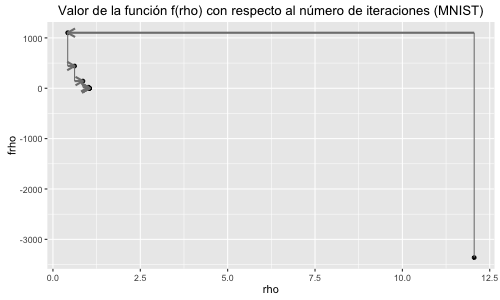
\includegraphics[width=.75\textwidth]{Figures/Chapter4_Iteraciones.png}	
  \caption[Valores de $\rho$ y $f(\rho)$ para distintas iteraciones (MNIST).] 
  {Valores de $\rho$ y $f(\rho)$ para distintas iteraciones (MNIST). El punto rojo es el punto inicial. Datos del conjunto de entrenamiento.}
\end{figure}

En la figura 3.3 se muestran $(\rho, f(\rho))$ para cada una de las 9 iteraciones. El punto inicial es el rojo, en este caso $\rho = 16.39$, mientras que $f(\rho)$ toma el valor de $-22,326$. Tras la primer iteración, $\rho$ toma el valor de $0.03$, y $f(\rho)$ es igual $42,841$. Conforme hay más iteraciones, $\rho$ y $f(\rho)$ convergen a los óptimos.

\underline{\textbf{3) Datos proyectados en 4 dimensiones}}

Se maximizó la traza del cociente para un espacio de 20 dimensiones. En la figura 3.4 se muestra como se agrupan los individuos del conjunto de entrenamiento conforme las iteraciones avanzan. 
  
\begin{figure}[!ht] \label{fig5.4}
  \centering
	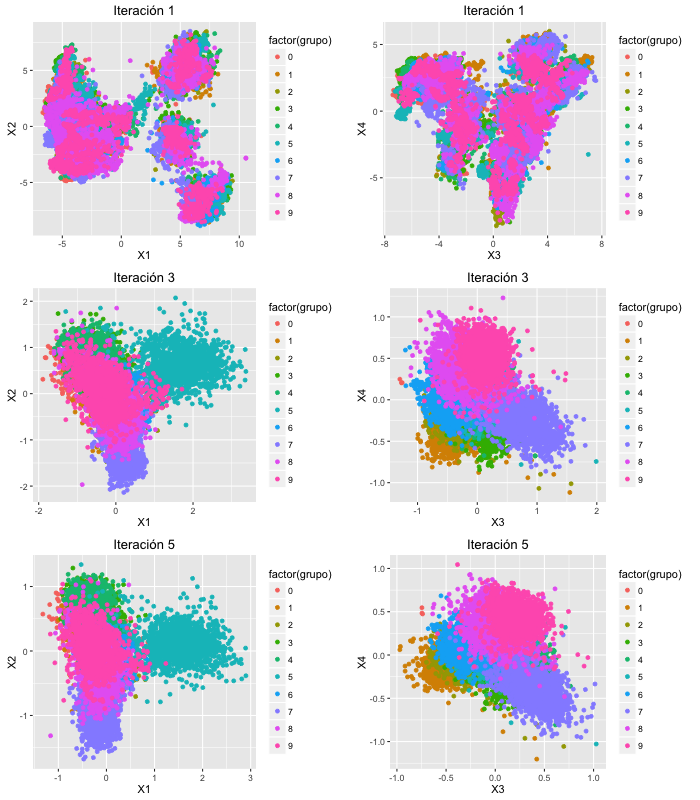
\includegraphics[width=1\textwidth]{Figures/Chapter4_ejemplo20componentes.png}	
  \caption[Ejemplo de proyección en 20 dimensiones (MNIST).]
  {Ejemplo de proyección en 20 dimensiones (MNIST). Las dos imágenes superiores son los datos de entrenamiento proyectadas sobre las 4 primeras componentes tras la primer iteración. Las dos intermedias son en la iteración 3 y las últimas 2 son la última iteración. Datos del conjunto de entrenamiento.}
\end{figure}

\subsection{Comparación con otros métodos}

Para la comparación de Newton-Lanczos con la RLM y el ADL se tomaron las siguientes consideraciones:

\begin{itemize}
\item Las dimensiones a considerar (k) son: 2, 5, 10, 15, 20, 40, 60, 80, 100, 120, 140, 160, 180 y 193
\item El número de variables que entran en cada modelo es el mismo (dada la dimensión k)
\item Los modelos se ajustan con el conjunto de entrenamiento y se calcula el error con el de prueba
\item Para Newton-Lanczos y ADL se proyectarán a un espacio k-dimensional y se usará 3-vecinos más cercanos para clasificarlos
\item Para el caso de regresión logística multinomial se elegirá la clase que tenga una mayor probabilidad posterior de selección
\end{itemize}

\underline{\textbf{1) Tasa de reconocimiento}}

La tasa de reconocimiento se mide como el número de individuos clasificados correctamente entre el número total del conjunto de test. Como el objetivo de esta sección es observar como se modifica la tasa con respecto aumenta k, se fijó el número de vecinos más cercanos a 3 para el caso de ADL y de Newton-Lanczos y también el tamaño del conjunto de entrenamiento. En la figura 3.5 se muestra que el modelo RLM y el ADL se comportan mejor para dimensiones pequeñas. Para casos de k mayor a 120, el método de Newton-Lanczos alcanza una mejor tasa de reconocimiento.

Es interesante observar que si se busca la mejor proyección con para k = 1 y k = 2, Newton-Lanczos resulta ser muy buen método. En la 3.4 se observó como los individuos se agrupan con este método. 


\begin{figure}[!ht] \label{fig5.5}
  \centering
	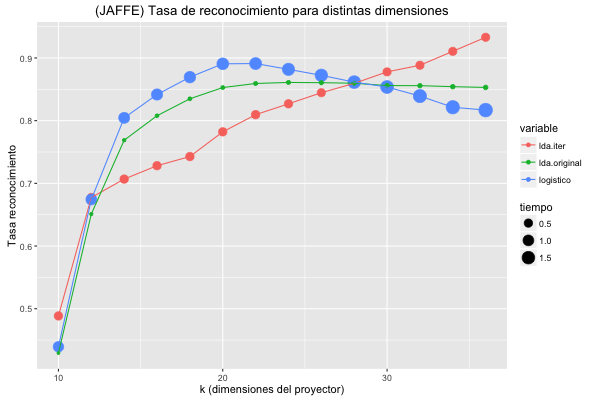
\includegraphics[width=1\textwidth]{Figures/Chapter4_Comparacion.png}	
  \caption[Tasa de reconocimiento base (MNIST).]
  {Tasa de reconocimiento base (MNIST). En azul se representa el RLM, en verde el ADL y en rojo el método de Newton-Lanczos. En el eje $y$ se muestra la tasa de reconocimiento y en el eje $x$ la dimensión a considerar (k). El tamaño representa el tiempo. Datos del conjunto de prueba.}
\end{figure}

\pagebreak
\underline{\textbf{2) Tiempo de ejecución}}

A continuación, se comparan los tiempos de ejecución de cada método. Para comparar los tiempos de ejecución justamente, se tomaron 3 distintos:

\begin{itemize}
\item 1) (PCA) Tiempo para calcular los componentes principales del conjunto de entrenamiento
\item 2) (Proyectar) Tiempo para calcular la proyección del conjunto de test
\item 3) (Modelo) Tiempo necesario para hacer las operaciones de cada método

\end{itemize}

\begin{center}
\begin{tabular}{ | c | c |} 
\hline
 PCA(s) & Proyectar(s) \\ 
\hline
\hline
$11.728$ & $21.680$ \\ 
\hline
\hline
\end{tabular}
\end{center}

La siguiente tabla muestra los tiempos de cómputo para los 3 métodos y con distinto número de componentes. 

\begin{center}
\begin{tabular}{ | c | c | c | c ||| c | c | c | c |} 
\hline
Comp & lda.iter & logístico & lda.orig   & Comp & lda.iter & logístico & lda.orig   \\ 
\hline
\hline
$2$ & $0.9092$ & $0.2712$ & $0.01$ & $80$ & $0.9222$ & $4.3186$ & $0.2684$ \\
$5$ & $0.8576$ & $0.5188$ & $0.0466$ & $100$ & $0.8764$ & $5.6474$ & $0.3572$ \\
$10$ & $0.864$ & $1.0646$ & $0.025$ & $120$ & $0.8952$ & $8.1026$ & $0.4942$ \\
$15$ & $0.8768$ & $1.103$ & $0.0372$ & $140$ & $0.9016$ & $9.2944$ & $0.7902$ \\
$20$ & $0.8886$ & $1.2888$ & $0.0524$ & $160$ & $0.8782$ & $10.1534$ & $0.908$ \\
$40$ & $0.886$ & $2.5528$ & $0.1004$ & $180$ & $0.898$ & $12.0426$ & $1.0596$ \\
$60$ & $0.8728$ & $3.2034$ & $0.1744$ & $193$ & $0643$ & $14.2512$ & $1.2186$ \\
\hline
\hline
\end{tabular}
\end{center}

El tiempo está en segundos (s).

Para cada iteración del método de Newton-Lanczos, se calcularon todos los eigenvalores ya que al no calcularlos, solo se tendrá una aproximación a sus valores y sus eigenvectores. Por este motivo, se decidió sacrificar tiempo de cómputo por precisión.

\pagebreak
\section{Base de datos JAFFE}


Ahora se analizará la base JAFFE \textit{Japanese Female Facial Expression}, que consta de 213 fotos provenientes de 10 personas distintas. Este conjunto de datos fue creado inicialmente para clasificar emociones, pero se usa comúnmente para probar otros tipos de algoritmos de clasificación. En nuestro caso será usado para clasificar el rostro de la persona, de esta manera se tendrán 10 clases. La base fue creada por Michael Lyons, Miyuki Kamachi y Jiro Gyoba en el departamento de psicología de la universidad de Kyushu. Puede descargarse de la página Web \textit{www.kasrl.org/jaffe.html}, cuyo link sigue vigente al 13 de marzo del 2016.

Las imágenes se encuentran en un formato \textit{.tiff}, por lo que se requirió la función \textit{readTIFF} del paquete $tiff$ el cual permite leerlas y convertirlas en un formato \textit{.RData}. La figura 3.6 contiene un extracto de tamaño 35 de la base original.

\begin{figure}[!ht]
  \centering
  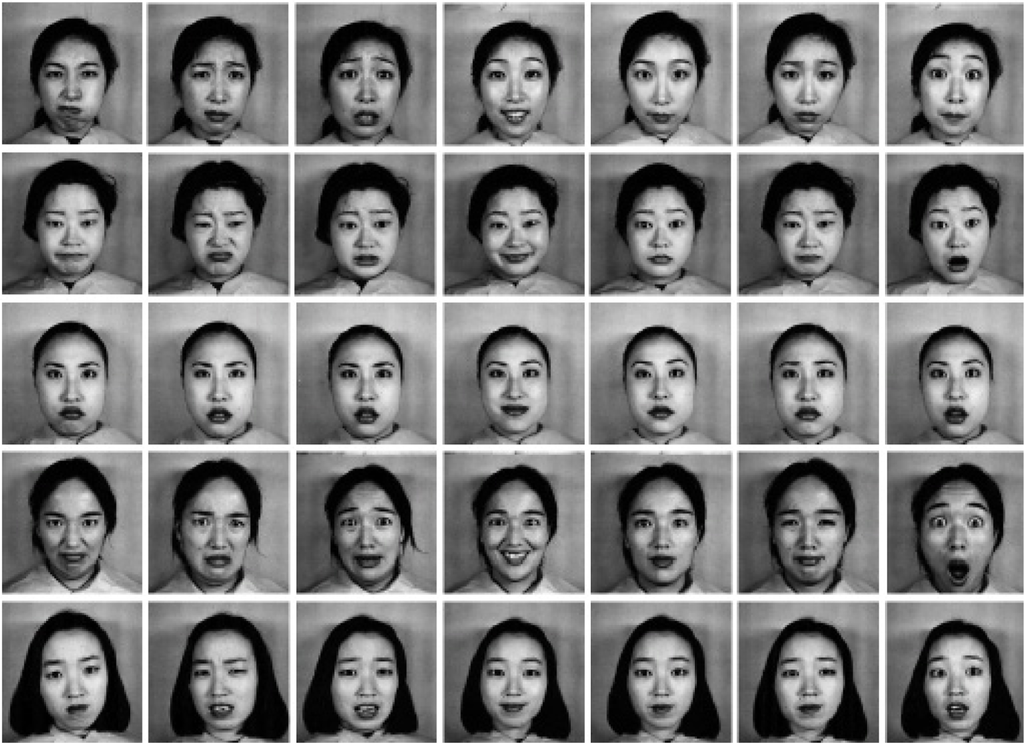
\includegraphics[width=.8\textwidth]{Figures/Chapter4_Jaffe.png} 
  \caption{Ejemplo de la base de datos (JAFFE).}
\end{figure}

\pagebreak
\subsection{Proyección sobre un espacio de dimensión 20}

\underline{\textbf{1) Cotas para $\rho^*$}}

Al igual que el ejemplo de MNIST, se ejemplificará la segunda cota presentada en el capítulo 2. Para esto se calcularon los eigenvalores de la matriz intraclase (B) y de la matriz entre clases (A). Los 20 eigenvalores más grandes y más pequeños de la primera son: \footnote{los eigenvalores menores a $1e^{-10}$ se consideraron numéricamente como 0}

\begin{center}
\begin{tabular}{ | c | c|  c |c | c|  c |c | c|  c |c | c | c|  c |c | c|  c |c | c|  c |c |} 
\hline
5303 & 4627 & 2083 & 1556 & 1370 & 1177 & 851 & 781 & 740 & 705 \\
629 & 596 & 562 & 520 & 498 & 466 & 453 & 403 & 397 & 382 \\
\hline
\hline
\end{tabular}
\end{center}

\begin{center}
\begin{tabular}{ | c | c|  c |c | c|  c |c | c|  c |c | c | c|  c |c | c|  c |c | c|  c |c |} 
\hline
250 & 245 & 231 & 223 & 219 & 203 & 198 & 192 & 176 & 147 \\
141 & 0 & 0 & 0 & 0 & 0 & 0 & 0 & 0 & 0 \\
\hline
\hline
\end{tabular}
\end{center}

De la misma manera, se calculan los 9 eigenvalores más grandes de la matriz entre clases (Los demás son 0):

\begin{center}
\begin{tabular}{ | c | c|  c |c | c|  c |c | c|  c |} 
\hline
14051 & 12922 & 7775 & 3247 & 3138 & 2849 & 1918 & 1336 & 1317 \\
\hline
\hline
\end{tabular}
\end{center}

Usando las formulas del capítulo 2, se tienen las siguientes cotas para $\rho^*$:

\begin{equation*}
\frac{\sum_{i = 1}^{p}\lambda_{A_i}}{\sum_{i = 1}^{p}\lambda_{B_i}} \leq \rho^* \leq \frac{\sum_{i = 1}^{p}\lambda_{(A)_i}}{\sum_{i = 1}^{p}\lambda_{(B)_{n-i+1}}}  
\end{equation*}

\begin{equation*}
\frac{48553}{24099} \leq \rho^* \leq \frac{48553}{2225}
\end{equation*}

\begin{equation*}
2.0147 \leq \rho^* \leq 21.8216
\end{equation*}


\pagebreak
\underline{\textbf{2) Valores de $(\rho^*, f(\rho^*))$}}

En la figura 3.7 se observa fácilmente rapidez de convergencia. En esta gráfica se muestra en el eje $y$ la raíz cuadrada de $f(\rho)$. Los criterios de paro se fijaron iguales que el ejemplo pasado (tol: $1e^{-10}$ y menos de 50 iteraciones). Para la base de JAFFE, se encontraron los siguientes resultados:

\begin{center}
\begin{tabular}{ | c | c|  c |} 
\hline
$iter$ & $\rho$ & $f(\rho)$  \\ 
\hline
\hline
1 & $11.88493$ & $6093.742$  \\ 
\hline
2 & $14.33840$ & $80.44169$  \\ 
\hline
3 & $14.37160$ & $.01093739e$  \\ 
\hline
4 & $14.37161$ & $1.873559 e^{-10}$  \\ 
\hline
\hline
\end{tabular}
\end{center}

\begin{figure}[!ht]
  \centering
  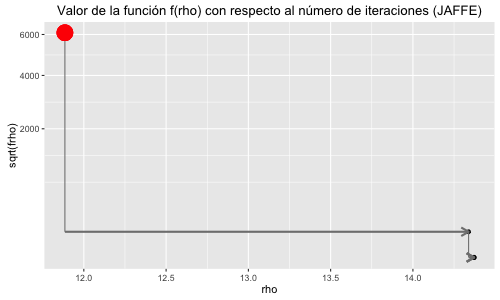
\includegraphics[width=.75 \textwidth]{Figures/Chapter4_Iteraciones_JAF.png} 
  \caption[Valores de $\rho$ y $f(\rho)$ para las iteraciones (JAFFE).]
  {Valores de $\rho$ y $f(\rho)$ para las iteraciones (JAFFE). El punto rojo es el punto inicial. Datos del conjunto de entrenamiento.}
\end{figure}

Se ve que la convergencia cuadrática del método de Newton ayuda a que se alcance el óptimo en pocas iteraciones. En la cuarta iteración $f(\rho)$ ya toma el valor de $1.87 e^{-10}$, muy cercano a 0. 

\pagebreak
\underline{\textbf{3) Datos proyectados en 4 dimensiones}}

De nuevo se maximizó la traza del cociente para un espacio de 20 dimensiones. En la figura 3.8 se muestra como se agrupan los individuos del conjunto de entrenamiento conforme las iteraciones avanzan.

\begin{figure}[!ht]
  \centering
  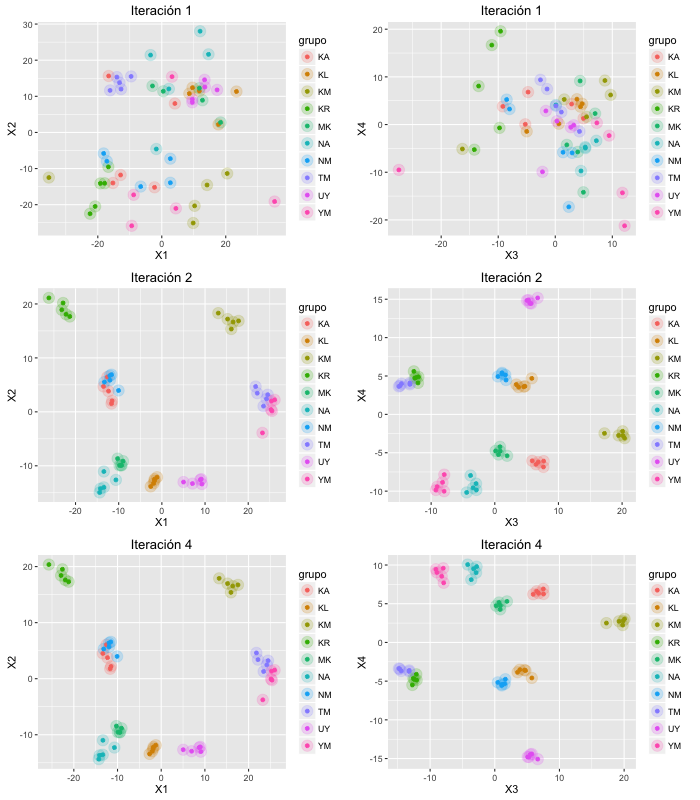
\includegraphics[width=1\textwidth]{Figures/Chapter4_ejemplo20componentes_JAF.png} 
  \caption[Ejemplo de proyección en 20 dimensiones (JAFFE).]
  {Ejemplo de proyección en 20 dimensiones (JAFFE). Las dos imágenes superiores son los datos de entrenamiento proyectadas sobre las 4 primeras componentes tras la primer iteración. Las dos intermedias son en la iteración 3 y las últimas 2 son la última iteración.}
\end{figure}


\subsection{Comparación con otros métodos}

De la misma forma que el ejemplo pasado se compararon los métodos en este caso. Lo único distinto serán las dimensiones a considerar k = 10, 13, 16, 19, 22, 25, 28, 31, 34, 37, 40, 43, 46 y 49. 

\underline{\textbf{1) Tasa de reconocimiento}}

\begin{figure}[!ht]
  \centering
  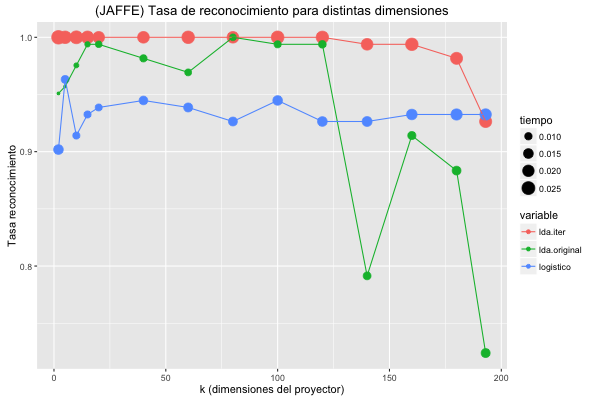
\includegraphics[width=1\textwidth]{Figures/Chapter4_Comparacion_Jaf.png} 
  \caption[Tasa de reconocimiento base (JAFFE)]
  {Tasa de reconocimiento base (JAFFE). En azul se representa el RLM, en verde el ADL y en rojo el método de Newton-Lanczos. En el eje $y$ se muestra la tasa de reconocimiento y en el eje $x$ la dimensión a considerar (k). El tamaño representa el tiempo. Se observa que en el ADL los últimos 4 puntos bajan la predicción. Esto es porque las variables son colineales y al calcular la inversa, causa inestabilidad numérica. Datos del conjunto de entrenamiento.}
\end{figure}

En la figura 3.9 se observa que el método de lda iterativo no tiene ningún error de clasificación para espacios de proyección menor a 40 dimensiones, reduciéndose en espacios de proyección con dimensión más alta. Esto puede deberse a que las últimas componentes son las menos discriminadoras, pero el método de 3-vecinos más cercanos las pondera igual. Una posible modificación que se puede realizar, es ponderar cada componente de acuerdo al poder discriminativo del correspondiente eigenvector.

En la figura 3.10 se muestran las últimas 4 componentes. Se observa que los individuos ya no están tan agrupados como en las primeras 4, por lo que el clasificador de 3-vecinos más cercanos podría no estar funcionando bien para $k > 40$.

\begin{figure}[!ht]
  \centering
  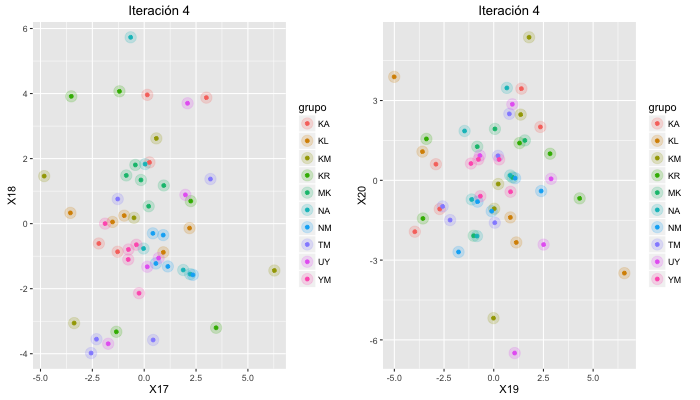
\includegraphics[width=.95\textwidth]{Figures/Chapter4_ultimasComponentes_JAF.png} 
  \caption[Individuos proyectados (JAFFE).]
  {Individuos proyectados (JAFFE). Conjunto de entrenamiento proyectados sobre las ultimas 4 componentes (17,18,19,20). Se observa que los grupos siguen estando relativamente cerca, pero si se toma 3-vecinos más cercanos no necesariamente se escogerá la persona correcta.}
\end{figure}


\underline{\textbf{2) Tiempo de ejecución}}
A continuación, se comparan los tiempos de ejecución de cada método. Para compararlos justamente, se tomaron 3 fases distintas y se comparó solamente el tiempo del modelo.

\begin{itemize}
\item 1) (PCA) Tiempo para calcular los componentes principales del conjunto de entrenamiento
\item 2) (Proyectar) Tiempo para calcular la proyección del conjunto de test
\item 3) (Modelo) Tiempo necesario para hacer las operaciones de cada método

\end{itemize}

\begin{center}
\begin{tabular}{ | c | c |} 
\hline
 PCA(s) & Proyectar(s) \\ 
\hline
\hline
$4.666$ & $4.801$ \\ 
\hline
\hline
\end{tabular}
\end{center}


\begin{center}
\begin{tabular}{ | c | c | c | c ||| c | c | c | c |} 
\hline
Comp & lda.iter & logístico & lda.orig   & Comp & lda.iter & logístico & lda.orig   \\ 
\hline
\hline
$10$ & $0.0352$ & $0.0098$ & $0.0068$ & $31$ & $0.0312$ & $0.0436$ & $0.0136$ \\
$13$ & $0.0324$ & $0.0146$ & $0.0074$ & $34$ & $0.0314$ & $0.0176$ & $0.0134$ \\
$16$ & $0.0378$ & $0.018$ & $0.0082$ & $37$ & $0.0314$ & $0.0224$ & $0.0144$ \\
$19$ & $0.031$ & $0.0114$ & $0.0104$ & $40$  & $0.0312$ & $0.0266$ & $0.0152$ \\
$22$ & $0.0308$ & $0.0128$ & $0.0112$ & $43$ & $0.0294$ & $0.0248$ & $0.0164$ \\
$25$ & $0.0326$ & $0.0136$ & $0.0102$ & $46$ & $0.03$ & $0.0228$ & $0.0188$ \\
$28$ & $0.0318$ & $0.0158$ & $0.0112$ & $49$ & $0.0204$ & $0.0594$ & $0.0176$ \\
\hline
\hline
\end{tabular}
\end{center}

El tiempo está en segundos (s).

Para cada iteración del método de Newton-Lanczos, se calcularon todos los eigenvalores (Excepto si el número de eigenpares a calcular es menor al 5\% del total) ya que al no calcular todos, solo se tendrá una aproximación a sus valores y sus eigenvectores. Por este motivo, se decidió sacrificar tiempo de cómputo por precisión.




	\chapter{Conclusiones}
\label{ch:conclusion}

% Párrafo intro 
En este trabajo se expone la técnica de optimización de Newton-Lanczos aplicada al problema de aprendizaje supervisado del Análisis Discriminante Lineal de Fisher (ADLF). El ADLF busca encontrar la mejor matriz de proyección que maximice el cociente de trazas, logrando que los individuos de una misma clase sean proyectados lo más cercano posible entre ellos y lo más separado posible de otra clase. Anteriormente, la solución era considera computacionalmente costosa de resolver; sin embargo, en la actualidad se puede aprovechar la velocidad de convergencia del método de Newton y la rapidez del algoritmo de Lanczos para calcular eigenpares. 

% ------ primero

El método de Lanczos es muy efectivo para calcular solamente algunos de los eigenpares de las matrices. Bajo el contexto de aritmética inexacta, Lanczos implementado con reortogonalización completa resulta ser más eficiente que la factorización SVD, cuando se desea calcular menos del 5 \% de los eigenpares. Aunque este número parece ser demasiado pequeño resulta de gran utilidad; por ejemplo, si la matriz tiene dimensión de $1000 \times 1000$, tener 50 eigenpares podría ser adecuado para el problema. 

\newpage
En este trabajo de tesis se comparó el método ADLF vía Newton-Lanczos con el Análisis Discriminante Lineal (ADL) y la técnica de Regresión Lineal Múltiple (RLM). La comparación se realizó empleando las bases JAFFE y MNIST. Los resultados obtenidos con ADLF vía Newton-Lanczos tuvieron un desempeño similar en comparación con los otros métodos en términos de tasa de reconocimiento y tiempo de cómputo.

Las conclusiones más relevantes de esta tesis son las siguientes:

\begin{itemize}
\item Se implementó computacionalmente una técnica de optimización que anteriormente resultaba difícil de resolver.
\item Una de las principales ventajas de esta metodología es que no requiere ningún supuesto sobre la distribución de los datos.
\item Se evaluó el desempeño de esta metodología con respecto a técnicas conocidas y los resultados fueron satisfactorios.
\item Se realizaron dos pruebas diferentes y se obtuvo que en algunos casos el ADLF vía Newton-Lanczos tuvo una precisión mayor con respecto a los otros dos métodos.
\end{itemize}


% ------ Tercero
Una de las complicaciones del algoritmo de Lanczos es la reortogonalización de la base. En este estudio se utilizó el método de reortogonalización completa; sin embargo, existen modificaciones al algoritmo que pueden ser exploradas con el objetivo de lograr mayor eficiencia en términos computacionales. Por ejemplo, J.W. Demmel (1997) \cite{demmel1997applied} propone algunas alternativas que pueden ser utilizadas para mejorar el proceso de reortogonalización de la base en el algoritmo de Lanczos.




		
	\appendix
	 \chapter{Apéndice A: Optimización de $Tr(V^TA V)$}
\label{ch:appendixA}


Sea $A \in {\rm I\!R}^{nxn}$ una matriz simétrica cuya factorización espectral es:

\begin{equation*}
\begin{aligned}
	A =& U^T \Lambda U \qquad U^T U = I_n\\
	\Lambda =& diag(\lambda_{A_1}, ..., \lambda_{A_n} )
\end{aligned}
\end{equation*}

donde $\lambda_{A_1} \geq \lambda_{A_2} \geq ... \geq \lambda_{A_n}$ son los valores propios de $A$ y $U$ una matriz ortogonal. En este apéndice se demostrará que:

\begin{equation}\label{A1:1}
\begin{aligned}
\max_{\substack{V^T V = I \\V \in {\rm I\!R}^{nxp} }}Tr(V^T A V) = \lambda_{A_1} + \lambda_{A_2} + ... + \lambda_{A_p}
\end{aligned}
\end{equation}

\section{Problema relajado}
Sean $\mathcal{U}_p$ y $\mathcal{V}_p$ dos conjuntos de matrices en ${\rm I\!R}^{nxp}$ tales que:

\begin{equation*}
\begin{aligned}
\mathcal{U}_p =& \{V \in {\rm I\!R}^{nxp} | V^TV = I_p\}	\\
\mathcal{V}_p =& \{V \in {\rm I\!R}^{nxp} | diag(V^TV) = I_p\}	
\end{aligned}
\end{equation*}

El conjunto $\mathcal{V}_p$ contiene a todas las matrices donde que cada columna tiene norma euclidiana igual a 1.

\begin{lemma}
El conjunto $\mathcal{V}_p$ es compacto en ${\rm I\!R}^{nxp}$
\begin{proof}
Por definición, si $V \in \mathcal{V}_p$ entonces $||V||_F = \sqrt(p)$.
Más aún, $\mathcal{V}_p$ contiene todos sus puntos límite.
\end{proof}
\end{lemma}

Si se relaja el problema original como:
\begin{equation} \label{A1:2}
	\max_{V \in \mathcal{V}_p} Tr(V^T A V)
\end{equation}
Como $\mathcal{V}_p$ es un conjunto compacto, la función continua $Tr(V^T AV)$ alcanza su valor máximo (o mínimo) en este conjunto. Ahora, como $\mathcal{U}_p \subset \mathcal{V}_p$, se tiene inmediatamente la desigualdad:

\begin{equation} \label{A1:3}
\max_{V \in \mathcal{U}_p} Tr(V^T A V) \leq \max_{V \in \mathcal{V}_p} Tr(V^T AV)	
\end{equation}

Por lo tanto, se se procede a establecer el siguiente resultado:

\begin{theorem}\label{A1:T1}
\begin{equation*}
	\max_{V \in \mathcal{V}_p} Tr(V^T A V) = \lambda_{A_1} + \lambda_{A_2} + ... + \lambda_{A_p}
\end{equation*}
\end{theorem}

\begin{proof}
Para $V \in \mathcal{V}_p$ con $V = (v_1 \enskip v_2 \enskip ...\enskip v_p)$ y $v_j$ la j-ésima columna de $V$. Se define el vector:

\begin{equation*}
	\mathbf{v} = (v_1^T\enskip v_2^T \enskip...\enskip v_p^T)^T \enskip \in \enskip {\rm I\!R}^{np}
\end{equation*}

o lo que es equivalente:
\begin{equation*}
\mathbf{v} = \left(\!
    \begin{array}{c}
		v_1 \\
		v_2 \\
		\vdots \\
		v_p \\
\end{array}
  \!\right) \quad
\end{equation*}

Entonces la $Tr(V^TAV) = v_1^TAv_1 + v_2^TAv_2 + ... + v_p^TAv_p$ y el problema \ref{A1:2} puede ser formulado como sigue:

\begin{equation} \label{A1:4}
	\max_{\substack{\mathbf{v}^T \mathbb{B}_j \mathbf{v} = 1 \\ j = 1, ..., p}} \mathbf{v}^T\mathbb{A} \mathbf{v}
\end{equation}

con las matrices $\mathbb{A}$ y $\mathbb{B}_j$:


\begin{equation*}
\mathbb{A} = \left(\!
    \begin{array}{cccccc}
		A & 0 & \hdots & 0 & \hdots & 0 \\
		0 & A & \hdots & 0 & \hdots & 0 \\
		\vdots & \vdots & \vdots & \vdots & \vdots & \vdots \\
		0 & 0 &  \hdots & A & \hdots & 0 \\
		\vdots & \vdots & \vdots & \vdots & \vdots & \vdots \\
		0 & 0 & \hdots & 0 & \hdots & A \\
\end{array}
  \!\right) \quad
\end{equation*}


\begin{equation*}
\mathbb{B}_j = \left(\!
    \begin{array}{cccccc}
		0 & 0 & \hdots & 0 & \hdots & 0 \\
		0 & 0 & \hdots & 0 & \hdots & 0 \\
		\vdots & \vdots & \vdots & \vdots & \vdots & \vdots \\
		0 & 0 &  \hdots & I_n & \hdots & 0 \\
		\vdots & \vdots & \vdots & \vdots & \vdots & \vdots \\
		0 & 0 & \hdots & 0 & \hdots & 0 \\
\end{array}
  \!\right) \quad
\end{equation*}

En ambas matrices hay $p$ bloques en los renglones y $p$ bloques en las columnas. Para $\mathbb{B}_j$ el bloque $(j,j)$ es $I_n$ y todos los demás son matrices cero. De esta manera, la función lagrangiana asociada al problema es:

\begin{equation*}
\mathcal{L}_j(\mathbf{v}, \eta) = \mathbf{v}^T \mathbb{A} \mathbf{v} - \sum\limits_{j=1}^{p}(\eta_j(\mathbf{v}^T\mathbb{B}_j\mathbf{v}-1))
\end{equation*}

Las condiciones de primer orden para la solución óptima son (considerando que $A$ es simétrica:
\begin{equation}\label{A1:5}
\begin{aligned}
	\nabla_{\mathbf{v}} \mathcal{L}(\mathbf{v}, \eta) =& \quad 2 \mathbb{A}\mathbf{v} - 2 \sum\limits_{j=1}^p (\eta_j(\mathbf{v}^T \mathbb{B}_j \mathbf{v})) = \quad 0 \\
	\nabla_{\eta_j} \mathcal{L}(\mathbf{v}, \eta)  =& \quad \mathbf{v}^T \mathbb{B}_j \mathbf{v} = 1 \quad con \quad j = 1, ...,p 
\end{aligned}
\end{equation}

De la primera ecuación de \ref{A1:5}, se tiene que:

\begin{equation*}
	\left(\mathbb{A}-\sum\limits_{j=1}^p \eta_j \mathbb{B}_j \right) v = 0
\end{equation*}

Donde la matriz $(\mathbb{A}-\sum\limits_{j=1}^p \eta_j \mathbb{B}_j)$ es diagonal a bloques. De hecho, el bloque $(j,j)$ es:

\begin{equation*}
(A-\eta_j I_n)v_j = 0 \quad \Rightarrow \quad Av_j = \eta_j v_j	
\end{equation*}

Entonces, $\eta_j$ debe ser un eigenvalor de A y $v_j$ su correspondiente eigenvector. Tomando de nuevo la ecuación de arriba, y multiplicándola por $v^T$ se obtiene:

\begin{equation*}
v^T \mathbb{A}v = \sum\limits_{j=1}^p (\eta_j)(v^T \mathbb{B}_j v)	
\end{equation*}

Ahora, usando la segunda ecuación de \ref{A1:5}, se tiene que:

\begin{equation*}
	v^T \mathbb{A}v = \sum\limits_{j=1}^p \eta_j
\end{equation*}

Por lo tanto, con el fin de maximizar la función $v^T \mathbb{A} v$ en $\mathcal{V}_p$, se deben escoger los primeros $p$ eigenvalores de la matriz A. Esto es:

\begin{equation*}
	\eta_j = \lambda_{A_j}, \qquad j = 1, ..., p
\end{equation*}

\end{proof}


Ahora, se tienen todas las piezas para demostrar el resultado principal.


\begin{theorem}\label{A1:T2}
\begin{equation*}
\max_{\substack{V^TV= I_p \\V \in {\rm I\!R}^{nxp}}} Tr(V^T A V)	= \lambda_{A_1} + \lambda_{A_2} + ... +\lambda_{A_p}
\end{equation*}
\end{theorem}

\begin{proof}
Se ha mostrado que:
\begin{equation*}
\max_{V \in \mathcal{U}_p} Tr(V^T A V)	\leq \lambda_{A_1} + \lambda_{A_2} + ... +\lambda_{A_p}	
\end{equation*}
\end{proof}

Considerando la matrix $U \in {\rm I\!R}^{nxn}$ de la factorización espectral de A, tal que $U = (u_1 \enskip u_2 \enskip ... \enskip u_n)$. Tomando las primeras $p$ columnas de $U$ se define $U^*$:



\begin{equation*}
\begin{aligned}
    U^* =& (u_1 \enskip u_2\enskip ...\enskip u_p) \quad con \quad U^* \in \mathcal{U}_p \quad y \\
	Tr(U^* A U) =& \lambda_{A_1} + \lambda_{A_2} + ... + \lambda_{A_p}
\end{aligned}
\end{equation*}



\section{Observaciones finales}

Se toman los resultados de la sección anterior para hacer las siguientes observaciones:


\begin{remark}
Se puede extender el último teorema, usando el mismo conjunto $\mathcal{V}_p$ y cambiando la maximización a minimización para obtener que:

\begin{equation}\label{A1:6}
\min_{V \in \mathcal{U}_p} Tr(V^T A V)	= \lambda_{A_n} + \lambda_{A_{n-1}} + ... +\lambda_{A_{n-(p-1)}}
\end{equation}
\end{remark}


\begin{remark}
Cuando $p = 1$, se pueden obtener las bien conocidas propiedades del cociente de Raleigh:

\begin{equation}\label{A1:7}
\begin{aligned}
\left(\min_{v^vv = 1} v^T A v	\right)=& \lambda_{A_n} \\
\left(\max_{v^vv = 1} v^T A v	\right)=& \lambda_{A_1}
\end{aligned}
\end{equation}
\end{remark}





	% \chapter{Apéndice B: Códigos en R}
\label{ch:appendixB}

\section{Experimentos numéricos}
\subsection{$01\_Prueba20comp$}

\begin{lstlisting}[language=R, basicstyle=\small]
library(ProjectTemplate)
reload.project()

# Jaffe.20 & Mnist.20  are 5 element lists:
# 1) iterative model
# 2) data frame with \rho, f\rho values
# 3) projection matrix V
# 4) test error
# 5) knn model

Jaffe.20 <- prueba.20comp(JAFFE.train, JAFFE.test, "JAFFE")
Mnist.20 <- prueba.20comp(MNIST.train, MNIST.test, "MNIST")

Jaffe.20$modelo.iterativo
Mnist.20$modelo.iterativo
\end{lstlisting}

\subsection{$02\_Models\_comparisons$}
\begin{lstlisting}[language=R, basicstyle=\small]
# 1) Data y proyeccion size --------------------------------
library(ProjectTemplate)
reload.project()

numComp.Jaffe <- c(10,13,16,19,22,25,28,31,
                   34,37,40,43,46,49) 
numComp.Mnist <- c(2,5,10,15,20,40,60,80,
                   100,120,140,160,180,193)

comp.error.MNIST<-comparacion.modelos(train.p = MNIST.train,
                                 test.p = MNIST.test, 
                                 dataset = "MNIST", 
                                 numComp = numComp.Mnist,
                                 fortran = FALSE)

comp.error.JAFFE<-comparacion.modelos(train.p = JAFFE.train,
                                  test.p = JAFFE.test, 
                                  dataset = "JAFFE", 
                                  numComp = numComp.Jaffe,
                                  fortran = FALSE)
# 2) Graphs ------------------------------------------------

graficar.comparacion(datos = comp.error.MNIST, 
                     numComp = numComp.Mnist, 
                     label = "MNIST")

graficar.comparacion(datos = comp.error.JAFFE, 
                     numComp = numComp.Jaffe, 
                     label = "JAFFE")
\end{lstlisting}

\subsection{$03\_Profiling$}
\begin{lstlisting}[language=R, basicstyle=\small]
# 1) Data y proyeccion size --------------------------------
library(ProjectTemplate)
reload.project()

# 1) Componentes ------------------------------------------
numComp.Jaffe <- c(10,13,16,19,22,25,28,31,
                   34,37,40,43,46,49) 
numComp.Mnist <- c(2,5,10,15,20,40,60,80,
                   100,120,140,160,180,193)
# 2) Profiling ----------------------------------------
prof.Mnist <- prolifiling.model(train.p = MNIST.train, 
                                test.p = MNIST.test,
                                dataset = "MNIST",
                                numComp = numComp.Mnist)
prof.Jaffe <- prolifiling.model(train.p = JAFFE.train, 
                                test.p = JAFFE.test,
                                dataset = "JAFFE",
                                numComp = numComp.Jaffe)

# 3) Graphs -------------------------------------------
graficar.profiling(times.profiling = prof.Mnist, 
                   numComp = numComp.Mnist, 
                   dataset = "MNIST")
graficar.profiling(times.profiling = prof.Jaffe, 
                   numComp = numComp.Jaffe, 
                   dataset = "JAFFE")
\end{lstlisting}

\section{Funciones}
\subsection{$load\_libraries$}
\begin{lstlisting}[language=R, basicstyle=\small]
# 1) Load libraries ----------------------------------------
set.seed(12345)
library(plyr) # Tools for split, applying and combine data
library(dplyr) # package of grammar of data manipulation
library(tidyr) # package to efficiently "tidy" data
library(FactoMineR) # Package for multivariate analysis
library(ggplot2) # Graphing package "Grammar of Graphics"
library(gridExtra) # Package to work with grid graphics
library(class) # Functions for classification, including knn
library(nnet) # Software for multinomial linear models
library(MASS) # "Applied Statistics with S"



# 1) Fisher eficiente ---------------------------------
lda.iter.ef <- function (test.p, 
                         train.p, 
                         espacio.proy,
                         prior = proportions,
                         tol = 1e-10) {
  
  # Prepare matrix of data
  x <- train.p %>% dplyr::select(-grupo)
  x <- as.matrix(x)
  
  # Get dimensions
  n <- nrow(x)
  p <- ncol(x)
  
  # Get number of groups and the levels
  g <- as.factor(train.p$grupo)
  lev <- lev1 <- levels(g)
  
  # Get the number of images per class
  counts <- as.vector(table(g))
  proportions <- counts/n
  ng <- length(proportions)
  names(prior) <- names(counts) <- lev1
  
  # Group means and total mean
  group.means <- tapply(c(x), list(rep(g, p), col(x)), mean)
  all.means <- as.matrix(colMeans(x)) %>% t()
  
  # Scatter Matrices 
  #Intra class
  B <- t(x - group.means[g, ]) %*% (x - group.means[g, ]) 
  # Between class
  A <- (t(group.means)-matrix(rep(all.means,10),ncol=10))%*% 
    diag(counts) %*% 
    t(t(group.means)-matrix(rep(all.means,10),ncol=10)) 
  
  # Initialization
  rhoAnt = -1000000
  iter=1
  dimension = espacio.proy
  # rho = (cota.inf + cota.sup)/2
  rho = 0
  frho = sum(eigen(A-rho*B)$values[1:dimension])
  V = eigen(A-rhoAnt*B)$vectors[,(1:dimension)]
  
  # list of results
  a=list()
  a[[1]] <- list(iter = 1, rho = rho, frho = frho, V = V) 
  
  # Iterative method (use of efficient irlba method)
  while(iter < 50 & abs(rho-rhoAnt)>tol){
    print(paste("iteracion: ",as.character(iter)))
    rhoAnt = rho
    iter=iter+1  
    V = eigen(A-rhoAnt*B)$vectors[,(1:dimension)] # Lanczos
    rho = sum(diag(t(V) %*% A %*% V)) /
    sum(diag(t(V) %*% B %*% V))
    frho = sum(eigen(A-rho*B)$values[1:dimension])
    a[[iter]] <- list(iter = iter, rho = rho,
                      frho = frho, V = V)
  }
  
  # Getting the projection matrix
  scaling <- V
  dimnames(group.means)[[2L]] <- colnames(x)
  cl <- match.call()
  cl[[1L]] <- as.name("lda.iter")
  structure(list(iteraciones = a, 
                 prior = prior, 
                 counts = counts, 
                 means = group.means, 
                 scaling = scaling, 
                 lev = lev, 
                 N = n, 
                 call = cl, 
                 class = "lda.iter"))
}

# 2) Fisher para pruebas ------------------------------
lda.iter <- function (test.p, 
                      train.p, 
                      espacio.proy,
                      prior = proportions, 
                      tol = 1e-10) {
  
  # Prepare matrix of data
  x <- train.p %>% dplyr::select(-grupo) %>% as.matrix()
  
  # Get dimensions
  n <- nrow(x)
  p <- ncol(x)
  
  # Get number of groups and the levels
  g <- as.factor(train.p$grupo)
  lev <- lev1 <- levels(g)
  
  # Get the number of images per class
  counts <- as.vector(table(g))
  proportions <- counts/n
  ng <- length(proportions)
  names(prior) <- names(counts) <- lev1
  
  # Group means and total mean
  group.means <- tapply(c(x), list(rep(g, p), col(x)), mean)
  all.means <- as.matrix(colMeans(x)) %>% t()
  
  # Scatter Matrices 
  #Intra class
  B <- t(x - group.means[g, ]) %*% (x - group.means[g, ]) 
  # Between class
  A <- (t(group.means)-matrix(rep(all.means,10),ncol=10))%*% 
    diag(counts) %*% 
    t(t(group.means)-matrix(rep(all.means,10),ncol=10)) 
  
  # [not run] Intra class + Between class = Total variance
  diag(A+B) 
  diag(49*(as.matrix(x) %>% cov))
  
  # [not run] EigenValues Time
  (eigen(B))$values
  (eigen(A))$values
  
  # [not run] Boundaries
  cota.inf <- sum((eigen(A))$values[1:espacio.proy])/
    sum((eigen(B))$values[1:espacio.proy])
  cota.sup <- sum((eigen(A))$values[1:espacio.proy])/
sum((eigen(B))$values[(dim(A)[1]+1-espacio.proy):dim(A)[1]])
  
  # Initialization
  rhoAnt = -1000000
  iter=1
  dimension = espacio.proy
  rho = (cota.inf + cota.sup)/2
  
  frho = sum(eigen(A-rho*B)$values[1:dimension])
  V = eigen(A-rhoAnt*B)$vectors[,(1:dimension)]
  
  # list of results
  a=list()
  a[[1]] <- list(iter = 1, rho = rho, frho = frho, V = V) 
  
  # Iterative method (use of efficient irlba method)  
  while(iter < 50 & abs(rho-rhoAnt)>tol){
    print(paste("iteracion: ",as.character(iter)))
    rhoAnt = rho
    iter=iter+1  
    V = eigen(A-rhoAnt*B)$vectors[,(1:dimension)]
rho = sum(diag(t(V)%*%A %*% V)) /sum(diag(t(V) %*% B %*% V))
    frho = sum(eigen(A-rho*B)$values[1:dimension])
a[[iter]] <-list(iter = iter, rho = rho, frho = frho, V = V)
  }
  
  # Getting the projection matrix
  scaling <- V
  dimnames(group.means)[[2L]] <- colnames(x)
  cl <- match.call()
  cl[[1L]] <- as.name("lda.iter")
  structure(list(iteraciones = a, 
                 prior = prior, 
                 counts = counts, 
                 means = group.means, 
                 scaling = scaling, 
                 lev = lev, 
                 N = n, 
                 call = cl, 
                 cota.inf = cota.inf, 
                 cota.sup = cota.sup, 
                 class = "lda.iter"))
}

# 3) LDA original -------------------------------------
lda.original <- function (x, 
                          grouping, 
                          prior = proportions, 
                          tol = 1e-04, 
                          nu = 5) {
  
  # Prepare matrix of data
  x <- as.matrix(x)
  n <- nrow(x)
  
  # Get dimensions
  p <- ncol(x)
  g <- as.factor(grouping)
  
  # Get number of groups and the levels
  lev <- lev1 <- levels(g)
  counts <- as.vector(table(g))
  
  # Get the number of images per class
  proportions <- counts/n
  ng <- length(proportions)
  names(prior) <- names(counts) <- lev1
  
  # Group means 
  group.means <- tapply(c(x), list(rep(g, p), col(x)), mean)
  f1 <- sqrt(diag(var(x - group.means[g, ])))
  scaling <- diag(1/f1, , p)
  
  # Calculate and project
  fac <-  1/(n - ng)
  X <- sqrt(fac) * (x - group.means[g, ]) %*% scaling
  X.s <- svd(X, nu = 0L)
  rank <- sum(X.s$d > tol)
  scaling <- scaling %*% X.s$v[, 1L:rank] %*% 
    diag(1/X.s$d[1L:rank], , rank)
  xbar <- colSums(prior %*% group.means)
  fac <-1/(ng - 1)
  X <- sqrt((n * prior) * fac) * scale(group.means, 
        center = xbar, scale = FALSE) %*% scaling
  X.s <- svd(X, nu = 0L)
  rank <- sum(X.s$d > tol * X.s$d[1L])
  scaling <- scaling %*% X.s$v[, 1L:rank]
  
  # Export
  dimnames(scaling) <- list(colnames(x), paste("LD",
          1L:rank, sep = ""))
  dimnames(group.means)[[2L]] <- colnames(x)
  cl <- match.call()
  cl[[1L]] <- as.name("lda")
  structure(list(prior = prior, counts = counts, 
                 means = group.means, 
                 scaling = scaling, lev = lev, 
                 svd = X.s$d[1L:rank], N = n, 
                 call = cl), class = "lda")
}

# 4) Lanczos Fortran -----------------------------------
# Give r0, A
lanczos.iter <- function(A){
  Dim = dim(A)[2]
  r0 = matrix(rep(0,Dim), ncol = 1)
  for(i in 1:Dim){
    r0[i] = runif(1, 0, 1) 
  }
r0 = r0 / sqrt(sum(r0^2))
r = list()
b = list()
a = list()
q = list()

q[[1]] = 0 # q0
r[[1]] = r0 #r0
b[[1]] = sqrt(sum(r[[1]]^2)) # b1
q[[2]] = as.matrix(r[[1]]/b[[1]], ncol =D) #q1
a[[1]] = t(q[[2]]) %*% A %*% q[[2]] #a1
q[[1]]
j <- 2
q = cbind(q[[1]], q[[2]])
while(b[[j-1]] > .0000001 | j < Dim+1){
  z = A %*% q[,j]
  z = z - q %*% (t(q) %*% z)
  z = z - q %*% (t(q) %*% z)
  b[[j]] = sqrt(sum(z^2))
  q.temp = z/b[[j]]
  q <- cbind(q, q.temp)
  a[[j]] = t(q[,j+1]) %*% A %*% q[,j+1]
  j = j+1
  print(j)
}

dyn.load("/usr/lib/liblapack.dylib")

Jobz <- as.character('V')#Get The eigenval and Eigenvector
N <- as.integer(Dim)#Matrix Dimension
D <- unlist(a)[1:Dim]#Diagonal
E <- unlist(b)[2:(Dim)]#Upper (and lower) diagonal
Z <- array(0.0,N*N)#storage for eigenvectors
Ldz <- N#Leading dimension of Z (in our case number of rows)
Work <- array(0.0,2*N)#Storage for processing
info <- as.integer(0)#Info flag

res<-.Fortran("dstev", Jobz, N, D, E, Z, Ldz, Work, info)

evalues <- res[[3]]
evectors <- matrix(res[[5]],N,N)
list(evalues, evectors)
}

# 5) Fisher eficiente ---------------------------------
lda.iter.fortran<- function (test.p = test.p, 
                         train.p = train.p, 
                         espacio.proy,
                         prior = proportions,
                         tol = 1e-10) {
  
  # Prepare matrix of data
  x <- train.p %>% dplyr::select(-grupo)
  x <- as.matrix(x)
  
  # Get dimensions
  n <- nrow(x)
  p <- ncol(x)
  
  # Get number of groups and the levels
  g <- as.factor(train.p$grupo)
  lev <- lev1 <- levels(g)
  
  # Get the number of images per class
  counts <- as.vector(table(g))
  proportions <- counts/n
  ng <- length(proportions)
  names(prior) <- names(counts) <- lev1
  
  # Group means and total mean
  group.means <- tapply(c(x), list(rep(g, p), col(x)), mean)
  all.means <- as.matrix(colMeans(x)) %>% t()
  
  # Scatter Matrices 
  #Intra class
  B <- t(x - group.means[g, ]) %*% (x - group.means[g, ]) 
  # Between class
  A <- (t(group.means)-matrix(rep(all.means,10),ncol=10))%*% 
    diag(counts) %*% 
    t(t(group.means)-matrix(rep(all.means,10),ncol=10)) 
  
  # Initialization
  rhoAnt = -1000000
  iter=1
  dimension = espacio.proy
  # rho = (cota.inf + cota.sup)/2
  rho = 0
  frho = sum(eigen(A-rho*B)$values[1:dimension])
  V = eigen(A-rhoAnt*B)$vectors[,(1:dimension)]
  
  # list of results
  a=list()
  a[[1]] <- list(iter = 1, rho = rho, frho = frho, V = V) 
  
  # Iterative method (use of efficient irlba method)
  while(iter < 50 & abs(rho-rhoAnt)>tol){
    print(paste("iteracion: ",as.character(iter)))
    rhoAnt = rho
    iter=iter+1  
    
  V = lanczos.iter(A-rhoAnt*B)[[2]][,(1:dimension)]#Lanczos
    rho = sum(diag(t(V) %*% A %*% V)) /
      sum(diag(t(V) %*% B %*% V))
    frho = sum(lanczos.iter(A-rhoAnt*B)[[1]][1:dimension])
    a[[iter]] <- list(iter = iter, rho = rho,
                      frho = frho, V = V)
  }
  
  # Getting the projection matrix
  scaling <- V
  dimnames(group.means)[[2L]] <- colnames(x)
  cl <- match.call()
  cl[[1L]] <- as.name("lda.iter")
  structure(list(iteraciones = a, 
                 prior = prior, 
                 counts = counts, 
                 means = group.means, 
                 scaling = scaling, 
                 lev = lev, 
                 N = n, 
                 call = cl, 
                 class = "lda.iter"))
}
\end{lstlisting}

\subsection{$functions\_comparison$}
\begin{lstlisting}[language=R, basicstyle=\small]
comparacion.modelos <- function(train.p, test.p, 
                                dataset,numComp, 
                                fortran = FALSE){
  # lda iterativo
  print(paste("===Corriendo el modelo con la base",dataset))
  
  lda.iter <- sapply(1:14, function(x){
    print(paste("Iteracion con: ", 
                numComp[x], 
                " componentes."))
    
    # Run model with different number of components
    if(fortran == FALSE){
    modelo.iterativo <- lda.iter.ef(train.p = train.p, 
                                    test.p = test.p, 
                                  espacio.proy = numComp[x])
    }else{
      modelo.iterativo <- lda.iter.fortran(train.p = train.p, 
                                      test.p = test.p, 
                                  espacio.proy = numComp[x])
    }
    # Data.frame with information of  (\rho and f(\rho))
    iter <- sapply(1:length(modelo.iterativo$iteraciones), 
                   function(x){
          data.frame(modelo.iterativo$iteraciones[[x]]$rho,
                  modelo.iterativo$iteraciones[[x]]$frho)%>% 
                setNames(c("rho", "frho")) %>% data.frame()
                   }) %>% t() %>% data.frame() %>% 
      mutate(iter = 1:nrow(.), 
             rho = unlist(rho),
             frho = unlist(frho))
    iter <- iter %>% data.frame() %>% 
      dplyr::mutate(frho2 = c(iter$frho[2:nrow(.)],NA ),
                    rho2 = c(iter$rho[2:nrow(.)], NA))
    
    # Projected data into a 20-dimensional space
    V <- modelo.iterativo$iteraciones[[
      length(modelo.iterativo$iteraciones)]]$V
    
    train.proyectados <- data.frame(as.matrix(train.p %>% 
                          dplyr::select(-grupo)) %*% V) %>%
      mutate(grupo = train.p$grupo)
    
    test.proyectados <- data.frame(as.matrix(test.p %>% 
                          dplyr::select(-grupo)) %*% V) %>%
      mutate(grupo = test.p$grupo)
    
    # K-nn model
    
    print("Iniciando modelo knn")
  modelo <- knn(train = train.proyectados[,c(1:numComp[x])], 
                test = test.proyectados[, c(1:numComp[x])], 
                  cl = train.proyectados$grupo, k = 3)
    pred <- data.frame(original = test.proyectados$grupo, 
                       predicho = modelo)
    
    pred <- pred %>% mutate(verdad = original != predicho)
    sum(pred$verdad)/nrow(pred)
  })
  
  modelo.logistico <- lapply(1:14, function(x){
    modelo <- multinom(grupo~., 
          data = train.p[,c(1:numComp[x], dim(train.p)[2])],
                       MaxNWts = 10000)
    predichos <- predict(modelo, 
                         newdata = test.p[,c(1:numComp[x])])
    pred <- data.frame(original = test.p$grupo, 
                       predicho = predichos)
    pred <- pred %>% mutate(verdad = original != predicho)
    sum(pred$verdad)/nrow(pred)
  })
  
  lda.original <- lapply(1:14, function(x){
    modelo<- lda(grupo ~ ., 
                 train.p[,c(1:numComp[x], 
                            dim(train.p)[2])], 
                 prior = c(1,1,1,1,1,1,1,1,1,1)/10)
  predichos <- predict(modelo, test.p[,1:numComp[x]])$class
    pred <- data.frame(original = test.p$grupo, 
                       predicho = predichos)
    pred <- pred %>% mutate(verdad = original != predicho)
    sum(pred$verdad)/nrow(pred)
  })
  
  data.frame(lda.iter = unlist(lda.iter), 
             logistico = unlist(modelo.logistico), 
             lda.original = unlist(lda.original))
}

graficar.comparacion <- function(datos, numComp, label){
  plot1 <- datos %>% 
    #write.table(sep = ';', pipe('pbcopy'), row.names= F)
    mutate(numComp = numComp) %>% 
    gather(variable, value, lda.iter:lda.original) %>% 
    ggplot(aes(x = numComp , y = 1-value, 
      group = factor(variable), color = factor(variable))) +
    geom_point() + geom_line()+
    labs(title = "Tasa de reconocimiento conforme 
         numero el espacio de proyeccion", 
         x = "numero de entrenamiento por grupo", 
         y="tasa reconocimiento")
  
  png(filename =paste(getwd(), "/graphs/Chapter4_comp_", 
        label, ".png", sep =""), width = 600,  height = 400)
  grid.arrange(plot1, ncol =1)
  dev.off()
}
\end{lstlisting}

\subsection{$functions\_prueba20comp$}
\begin{lstlisting}[language=R, basicstyle=\small]
# funciones prueba 20 componentes

plot.comp <- function(V1, label, train.p, test.p){
  train.proyectados <- data.frame(as.matrix(train.p %>% 
                          dplyr::select(-grupo)) %*% V1) %>%
    mutate(grupo = train.p$grupo)
  
  test.proyectados <- data.frame(as.matrix(test.p %>% 
                          dplyr::select(-grupo)) %*% V1) %>%
    mutate(grupo = test.p$grupo)
  
  a1 = ggplot(train.proyectados) + 
    geom_point(aes(x=X1, y=X2, 
                   group = grupo, color = grupo), 
               size=5, alpha = .2) + 
    geom_point(aes(x=X1, y=X2, 
                   group = grupo, color = grupo))+ 
    labs(title = label)
  a2 = ggplot(train.proyectados) + 
    geom_point(aes(x=X3, y=X4, 
                   group = grupo, color = grupo), 
               size=5, alpha = .2) + 
    geom_point(aes(x=X3, y=X4, 
                   group = grupo, color = grupo))+ 
    labs(title = label)
  list(a1,a2)
}
plot.ult <- function(V1, label, train.p, test.p){
  train.proyectados <- data.frame(as.matrix(train.p %>% 
                          dplyr::select(-grupo)) %*% V1) %>%
    mutate(grupo = train.p$grupo)
  
  test.proyectados <- data.frame(as.matrix(test.p %>% 
                          dplyr::select(-grupo)) %*% V1) %>%
    mutate(grupo = test.p$grupo)
  a7 =  ggplot(train.proyectados) + 
    geom_point(aes(x=X17, y=X18, 
                   group = grupo, color = grupo), 
               size=5, alpha = .2) + 
    geom_point(aes(x=X17, y=X18, 
                   group = grupo, color = grupo))+ 
    labs(title = label)
  
  a8 =  ggplot(train.proyectados) + 
    geom_point(aes(x=X19, y=X20, 
                   group = grupo, color = grupo), 
               size=5, alpha = .2) + 
    geom_point(aes(x=X19, y=X20, 
                   group = grupo, color = grupo))+ 
    labs(title = label)
  list(a7,a8)
}
prueba.20comp <- function(train.p, test.p, dataset){
  # Iterative LDA, projected to a 20-dimentional space
  modelo.iterativo <- lda.iter(train.p = train.p, 
                               test.p = test.p,
                               espacio.proy = 20)
  # Data.frame with information of (\rho and f(\rho))
  iter <- sapply(1:length(modelo.iterativo$iteraciones), 
                 function(x){
          data.frame(modelo.iterativo$iteraciones[[x]]$rho,
                modelo.iterativo$iteraciones[[x]]$frho)  %>% 
                     setNames(c("rho", 
                            "frho")) %>% data.frame()}) %>% 
    t() %>% data.frame() %>% 
    mutate(iter = 1:nrow(.), 
           rho = unlist(rho),
           frho = unlist(frho))
  iter <- iter %>% 
    dplyr::mutate(frho2 = c(iter$frho[2:nrow(.)],NA),
                  rho2 = c(iter$rho[2:nrow(.)], NA))
  
  # f(\rho) graph. It contains the iterations of the algorit
  plot <- iter %>% ggplot() +
    geom_point(aes(x = rho, y = frho))  + 
    geom_segment(aes(x = rho, y = frho, 
                     xend = rho, yend = frho2), 
                 color = "gray50") +
    geom_segment(aes(x = rho, y = frho2, 
                     xend = rho2, yend = frho2), 
                 arrow = arrow(length = unit(.3, "cm")), 
                 size = 1, 
                 color = "gray50") +
    labs(title = paste("Valor de la funcion f(rho) con 
      respecto al numero de iteraciones ", dataset,sep =""), 
         ylab = "f(rho)",
         xlab = "rho")
  # Save the image into a *.png file
  png(paste(getwd(), "/graphs/Chapter4_iteraciones_", 
      dataset, ".png", sep =""),width = 500, height = 500)
  grid.arrange(plot, ncol = 1)
  dev.off()
  
  # Projected data into a 20-dimensional space
  V <- modelo.iterativo$iteraciones[[
    length(modelo.iterativo$iteraciones)]]$V
  
  r1 <- 1
  r2 <- round(length(modelo.iterativo$iteraciones)/3*1)
  r3 <- round(length(modelo.iterativo$iteraciones))
  
  # iteration1
  V1 <- modelo.iterativo$iteraciones[[r1]]$V
  plot1 <- plot.comp(V1, paste("Iteracion ",r1, sep=""),
                     train.p, test.p)
  
  # iteracion3
  V2 <- modelo.iterativo$iteraciones[[r2]]$V
  plot2 <- plot.comp(V2, paste("Iteracion ",r2, sep=""),
                     train.p, test.p)
  
  # iteracion9
  V3 <- modelo.iterativo$iteraciones[[r3]]$V
  plot3 <- plot.comp(V3, paste("Iteracion ",r3, sep=""),
                     train.p, test.p)
  
  png(paste(getwd(),"/graphs/Chapter4_ejemplo20componentes_",
        dataset, ".png", sep =""),width = 700, height = 800)
  grid.arrange(plot1[[1]],plot1[[2]],plot2[[1]],
               plot2[[2]],plot3[[1]],plot3[[2]], 
               ncol = 2)
  dev.off()
  
  # last components
  V4 <- modelo.iterativo$iteraciones[[r3]]$V
  plot4 <- plot.ult(V4, "Ultimas componentes", 
                    train.p, test.p)
  png(paste(getwd(),"/graphs/Chapter4_ultimasComponentes_",
        dataset, ".png", sep =""),height = 400, width = 700)
  grid.arrange(plot4[[1]],plot4[[2]], ncol = 2)
  dev.off()
  # knn model ---------------------------------------------
  V <- modelo.iterativo$iteraciones[[
    length(modelo.iterativo$iteraciones)]]$V
  
  train.proyectados <- data.frame(as.matrix(train.p %>% 
                          dplyr::select(-grupo)) %*% V) %>%
    mutate(grupo = train.p$grupo)
  
  test.proyectados <- data.frame(as.matrix(test.p %>% 
                          dplyr::select(-grupo)) %*% V) %>%
    mutate(grupo = test.p$grupo)
  
  train.proyectados %>% head
  knn.model <- knn(train = train.proyectados[,c(1:20)], 
                   test = test.proyectados[, c(1:20)], 
                   cl = train.proyectados$grupo, k = 3)
  
  pp <- data.frame(original = test.proyectados$grupo, 
                   predicho = knn.model)
  
  pp <- pp %>% mutate(verdad = original != predicho)
  
  error <- sum(pp$verdad)/nrow(pp)
  list(modelo.iterativo=modelo.iterativo,iter = iter, V = V, 
       error = error, knn.model = knn.model)
}
\end{lstlisting}

\subsection{$functions\_profiling$}
\begin{lstlisting}[language=R, basicstyle=\small]
prolifiling.model <- function(train.p, test.p, 
                                dataset,numComp){

print(paste("====Realizando profiling de la base",dataset))
lda.time <- lapply(1:14, function(x){
  print(paste("Iteracion con: ", 
              numComp[x], " componentes."))
  
  lda.iter <- sapply(1:5, function(y){
    system.time(modelo.iterativo <- 
                  lda.iter.ef(train.p = train.p, 
                              test.p = test.p, 
                              espacio.proy = numComp[x]))
  }) %>% data.frame() %>% t() %>% data.frame() %>% 
    dplyr::select(elapsed) %>% 
    dplyr::summarise(mean = mean(elapsed))
  
  logistico <- sapply(1:5, function(y){
    system.time(modelo <- multinom(grupo~., 
          data = train.p[,c(1:numComp[x], dim(train.p)[2])], 
                                   MaxNWts = 10000))
  }) %>% data.frame() %>% t() %>% data.frame() %>% 
    dplyr::select(elapsed) %>% 
    dplyr::summarise(mean = mean(elapsed))
  
  lda.original <- sapply(1:5, function(y){
    system.time(modelo <- lda(grupo ~ .,
                train.p[,c(1:numComp[x], dim(train.p)[2])], 
                        prior = c(1,1,1,1,1,1,1,1,1,1)/10))
  })  %>% data.frame() %>% t() %>% data.frame() %>% 
    dplyr::select(elapsed) %>% 
    dplyr::summarise(mean = mean(elapsed))
  
  list(lda.iter, logistico, lda.original)
})

data.frame(unlist(lda.time)) %>% 
  mutate(var = rep(c("lda.iter", "logis", "lda.orig"), 14),
         ID = rep(1:(nrow(.)/3), each = 3)) %>% 
  setNames(c("time", "var", "ID")) %>% 
  spread(var, time)
}


graficar.profiling <- function(times.profiling, numComp,
                               dataset){
plot1 <- times.profiling %>% 
  mutate(numComp = numComp) %>% 
  gather(variable, value, lda.iter:logis) %>% 
  ggplot(aes(x = numComp , y = value,
             group = variable, color = variable)) +
  geom_point() + geom_line()+
  labs(title = "Tiempo de los modelos", 
       x = "Espacio de proyeccion", 
       y="Tiempo en (s)")
png(filename = paste(getwd(), "/graphs/Chapter4_profiling", 
      dataset, ".png", sep =""), width = 600, height = 400)
grid.arrange(plot1, ncol = 1)
dev.off()
}
\end{lstlisting}

\section{Preprocesamiento}

\subsection{$MNIST\_munge$}
\begin{lstlisting}[language=R, basicstyle=\small]
# 1) Load libraries ----------------------------------------
set.seed(12345)
library(plyr) # Tools for split, applying and combine data
library(dplyr) # package of grammar of data manipulation
library(tidyr) # package to efficiently "tidy" data
library(FactoMineR) # Package for multivariate analysis
library(ggplot2) # Graphing package "Grammar of Graphics"
library(gridExtra) # Package to work with grid graphics

# 1) Generate train and test from MNIST (run once) ---------
# darch::readMNIST("data/MNIST/")

# 2) Read MNIST data ---------------------------------------
# Original datasets
load("data/MNIST/train.RData")
load("data/MNIST/test.RData")

# Matrix with images in the rows and the variable in columns
numeros.ind.pix = rbind(data.frame(trainData, 
                  grupo = factor(apply(trainLabels[,], 1,  
                      function(x){ which(x == 1)-1 }))),
                  data.frame(testData, 
                      grupo = factor(apply(testLabels[,], 1,  
                      function(x){ which(x == 1)-1 })))) %>% 
  mutate(ID = 1:nrow(.))
base.mnist <- numeros.ind.pix
cache("base.mnist")
rm(testData, testLabels, trainData, trainLabels)

# 3) Train and test sets -----------------------------------
# Size of images per class
n.train <- 400

# Sample $n.train$ imager per class
train.id <- numeros.ind.pix %>% 
  group_by(grupo) %>% 
  sample_n(n.train) %>% 
  data.frame()

# Train and Test data.frames                    
train <- numeros.ind.pix[train.id$ID, ]
test <- numeros.ind.pix[-train.id$ID, ]

# Percentaje of images in train dataset
nrow(train)/(nrow(train)+nrow(test))

# 4) PCA ---------------------------------------------------
# PCA of MNIST dataset (each row is an image)
# 193 colums contains ~95% of the total variance
system.time(pca.train <- PCA(train %>% 
                               dplyr::select(-grupo, -ID), 
                             graph = F,
                             scale.unit = F,
                             ncp = 193))

# Matrix of loadings: 784 rows, 193 columns 
loadings <- sweep(pca.train$var$coord,2,  # 784 x 193
        sqrt(pca.train$eig[1:ncol(pca.train$var$coord),1]),
        FUN="/")

# Principal components 
train.p <- pca.train$ind$coord %>% data.frame() %>% 
  dplyr::mutate(grupo = train$grupo)

# [Revision] reconstuyendo primer componente 
as.matrix(scale(train %>% dplyr::select(-grupo, -ID), 
                center = apply(train %>% 
                      dplyr::select(-grupo, -ID), 2,mean), 
                scale = F)) %*% loadings[,1] %>% head

pca.train$ind$coord[,1] %>% head

# Projection of the test dataset with the train loadings 
# (centered with mean of train dataset)
system.time(test.p <- as.matrix(scale(test %>% 
            dplyr::select(-grupo, -ID), # 69,000 x 193
                                      
            center = apply(train %>% # centers of train
                    dplyr::select(-grupo, -ID), 2,mean), 
                          scale = F)) %*% loadings %>% 
              data.frame() %>% 
              mutate(grupo = test$grupo))
dim(test.p)
dim(train.p)
MNIST.test <- test.p
MNIST.train <- train.p
cache("MNIST.test")
cache("MNIST.train")
\end{lstlisting}

\subsection{$JAFFE\_munge$}
\begin{lstlisting}[language=R, basicstyle=\small]
# 1) Load libraries ----------------------------------------
set.seed(12345)
library(tiff) # package that reads *.tiff images 
library(tidyr) # package to efficiently "tidy" data
library(dplyr) # package of grammar of data manipulation
library(ProjectTemplate) # Template data analysis project
library(FactoMineR) # Package for multivariate analysis

# 2) Read databases ----------------------------------------
# Get the names of the files
files <- (Sys.glob("data/Jaffe/*.tiff"))

# Create an array that contains all the images paths 
nombres.personas <- apply(as.matrix(files),1,function(x){
  gsub("data/Jaffe/","",x)  
})

# Data.frame with info about each image (ID, name, class)
guia.personas.df <- data.frame(nombres.personas,
                               nombres.personas) %>%
  separate(nombres.personas.1, c("persona", 
                                 "postura", 
                                 "ID", 
                                 "extension")) %>%
  dplyr::select(-extension,
                -ID) %>%
  mutate(ID = 1:213, 
         nombres.personas = as.character(nombres.personas),
         persona = factor(persona),
         postura = factor(postura))

# List of length 213 that contains an image in each element
lista.completa.imagenes <- lapply(files, function(x){  
  imagen <- readTIFF(x)
  if(length(dim(imagen)) == 3){
    matrix <- as.vector(imagen[,,1])
  }else{
    matrix <- as.vector(imagen)
  }
})

# Data.frame, each column is an image
base.imagenes <- data.frame(lista.completa.imagenes)
names(base.imagenes) <- guia.personas.df$nombres.personas

# 2 matrices: In base.pix.ind.1, the columns are the images
#             In base.ind.pix.1, the rows are the images            
base.pix.ind.1 <- data.frame(base.imagenes)
base.ind.pix.1 <- data.frame(t(base.imagenes)) %>% 
  mutate(grupo = names(base.imagenes)) %>% 
  separate(grupo, c("grupo", 
                    "postura", 
                    "ID", 
                    "extension")) %>% 
  dplyr::select(-postura, 
                -ID, 
                -extension) %>% 
  mutate(ID = 1:nrow(.))

# 3) Explorar bases de datos -------------------------------
# sizes of the matrices
dim(base.pix.ind.1) # 65,536 rows and 213 columns
dim(base.ind.pix.1) # 213 rows and 65,536 columns

# save in cache the data.base
base.jaffe <- base.ind.pix.1
cache("base.jaffe")

# 4) Train and test  ---------------------------------------
# Size of images per class
n.train <- 5

# Sample $n.train$ imager per class
train.id <- base.jaffe %>% 
  group_by(grupo) %>% 
  sample_n(n.train) %>% 
  data.frame()

# Train and Test data.frames
train <- base.jaffe[train.id$ID, ]
test <- base.jaffe[-train.id$ID, ]

# Percentaje of images in train dataset
nrow(train)/(nrow(train)+nrow(test))

# 5) PCA ---------------------------------------------------

# PCA of JAFFE dataset (each row is an image)
# 52 colums contains ~95% of the total variance
system.time(pca.train <- PCA(train %>% 
                               dplyr::select(-grupo, -ID), 
                             graph = F,
                             scale.unit = F,
                             ncp = 49)) 

# Matrix of loadings: 65,536 rows, 49 columns
loadings <- sweep(pca.train$var$coord,2,
        sqrt(pca.train$eig[1:ncol(pca.train$var$coord),1]),
        FUN="/")

# Principal components 
train.p <- pca.train$ind$coord %>% data.frame() %>% 
  dplyr::mutate(grupo = train$grupo)

# [Revision] Reconstuyendo primer componente 
as.matrix(scale(train %>% dplyr::select(-grupo, -ID), 
                center = apply(train %>%
                        dplyr::select(-grupo, -ID), 2,mean), 
                scale = F)) %*% loadings[,1] %>% head

pca.train$ind$coord[,1] %>% head

# Projection of the test dataset with the train loadings 
# (centered with mean of train dataset)
system.time(test.p <- as.matrix(scale(test %>% 
                    dplyr::select(-grupo, -ID), 
                    center = apply(train %>% 
                       dplyr::select(-grupo, -ID), 2,mean), 
                    scale = F)) %*% loadings %>% 
              data.frame() %>% 
              mutate(grupo = test$grupo))

JAFFE.test <- test.p
JAFFE.train <- train.p
cache("JAFFE.test")
cache("JAFFE.train")

rm(list = ls())
\end{lstlisting}




	



	%%%%%%%%%%%%%%%%%%%%%%%%%%%%%%%%%%%%%%%%%%%%%%
	% VERSION ANTIGUA
	%%%%%%%%%%%%%%%%%%%%%%%%%%%%%%%%%%%%%%%%%%%%%%
 % 	\chapter{Prólogo}
\label{ch:prologo}

%\begin{chapterquote}{Leslie Lamport}
%	Formal mathematics is nature's way of letting you %know how sloppy
%your mathematics is.
%\end{chapterquote}

Esta tesis aborda el tema del Análisis Discriminante de Fisher. Este problema busca encontrar la proyección de los datos a un espacio p-dimensional que maximice el cociente de la matriz de dispersión entre-clases y la matriz de dispersión intra-clases. La solución era considerada computacionalmente costosa de encontrar, por lo que era remplazada por versiones simplificadas del problema.

En este texto, se aborda una propuesta de solución que es computacionalmente accesible. El costo es comparable con otros dos problemas de clasificación lineal que son mencionados en la literatura estadística, el análisis discriminante y la regresión logística multinomial. Las bases de datos que se utilizaron para comparar los métodos, fueron JAFFE y MNIST.

El segundo capítulo ubica el problema en el contexto del aprendizaje de máquina. Como primera instancia, se presenta dentro de los métodos de aprendizaje supervisado, para después ubicarlo en los problemas de clasificación lineal. Estos métodos pueden pertenecer a alguno de los siguientes tres grupos: métodos discriminativos, métodos generativos y funciones discriminantes. Al final del capítulo se introducen los criterios de selección, incluyendo el error de clasificación y la pérdida esperada. 

El tercer capítulo profundiza en el Discriminante Lineal de Fisher. Se presenta la dispersión interna, la dispersión entre clases y la dispersión total. Después, se encuentra la solución cuando el espacio a proyectar es de dimensión 1 y se generaliza a $p$ dimensiones. Al final del capítulo, se demuestra que el problema es equivalente a un problema escalar, por lo que se puede expresar en términos de una $f(\rho)$, una $\rho$ unidimensional. A continuación, se dan las condiciones de existencia de la solución y un intervalo en donde se encuentra el valor óptimo.

El cuarto capítulo introduce el método Newton-Lanczos para encontrar la $\rho$ óptima. Se da una breve presentación de la teoría que sustenta a los métodos de Lanczos, su costo computacional y las ventajas que tienen sobre los métodos tradicionales. En seguida de esto, se presenta la propuesta de solución: El método Newton-Lanczos. Este requiere el cómputo de la derivada de $f(\rho)$, por lo que se se calcula en este capítulo. Al final, se proporcionan las condiciones necesarias de optimalidad.

El quinto capítulo presenta los experimentos numéricos sobre las bases utilizadas. Se da una breve introducción de su preprocesamiento, para después continuar con un ejemplo donde se proyecta a una dimensión de tamaño 20. Al final del capítulo se compara el desempeño con el análisis discriminante lineal y con la regresión logística mulitinomial para diferentes $p$ y se mide el tiempo de cómputo.

Para todo el proyecto se utilizó el lenguaje de programación R y la paquetería \textit{ProjectTemplate}, que sirve para gestionar proyectos de análisis. Para asegurar la portabilidad y reproducibilidad del proyecto,
se utilizó la paquetería \textit{Packrat}. Por último, para los cálculos, se utilizó la biblioteca de \textit{LAPACK (Fortran)}  en su versión para OS X 10.11.4 (\textit{liblapack.dylib)}. 


	%   \chapter{Máquinas de aprendizaje}
\label{ch:chapter1}
 
Machine learning is founded in two research areas: Computer Sciences and Statistics. From the first, it takes the questions: How can we build machines that solves problems? and, Given the actual techonology, What kind of problems are feasibles to solve? On the other hand, from Statistics it tryes to answer: What conclusions can be infered from the dataset? and How can we manage the uncertainty of this method? \cite{mitchell2006discipline}. The joint work from both areas to try to answer these questions helps to build a computational statistical framework of machine learning.

\section{The process of learning}

A machine \textit{learns} given a task (T), a measure of the performance (R) and a type of experience (E) if the system improves the performance (R) in the task (T) with this expericence (E) \cite{mitchell2006discipline}. With the data, we try to model a structure in order that the machine improves their performance when it receives more information. The diversity of the task, as well as the applications is big. For example:

\begin{itemize} 

\item \textit{Spam/no-spam classification}, Here, (E) are the emails, (T) the task to classify correctly the \textit{spam} y (R) the proportion of correctly classified emails.

\item \textit{Face recognition/classification}, Here, (E) are the faces of distinct people, (T) is the correct classification of the faces and (R) is the measured as the percentage of correct classified faced.

\end{itemize} 

The learning proceses have many applications and distinct assumptions. For this reason, is useful to provide a framework that groups all the methods given some criteria. The classification used here is the proposed for T. Hastie \cite{hastie2009elements}. This divides the methods in two groups: Supervised learning and unsupervised learning. The first assumes the an output variable that helps to build the structure of the model. Examples of this are the Linear Regression, the decission and classification trees (CART) and the Support Vector Machines (SVM). On the other hand, the unsupervised learning only uses the information of the independent variables. For example, cluster análisis, asociation rules and some dimensiontality reduccion methods.

After this first classification, a subgroups are of the supervised methods are made depending of the output variable (Figura 1.1). \footnote{In this text will be used the terms input variable and ouput variables as the  dependant and independant variables respectively} When the model considers a quantitative variable, then it recives the name of regression, and when it is a categrical variable it receives the name of classification. On the other hand, the unsupervised learning have two main branches \cite{hastie2009elements}. The first is called segmentation, in which each individual is assigned to one group in a way that inside the group they are homogeneus between them, but between groups they are different. The second group of methods is the dimensitonality reduction, in which we try to project the individuals of the dataset into a much subspace of the space generated from the original dataset.

To give solution to classification problems there are different methods that can be compared, some of them are the Logistic Regression, the Linear Discriminant Analysis and the Support Vector Machines. On the other hand, if is a regreesion problem, the most comon approach are linear and non linar regression. There is another class of methods that is commonly used to solve both problems. These are the ensemble methods (random forest, boosting) that give a better precision, but with the cost of less interpretability. In this thesis a special enphasis will be given to the classification problems. 

\begin{figure}[!ht]
  \centering
	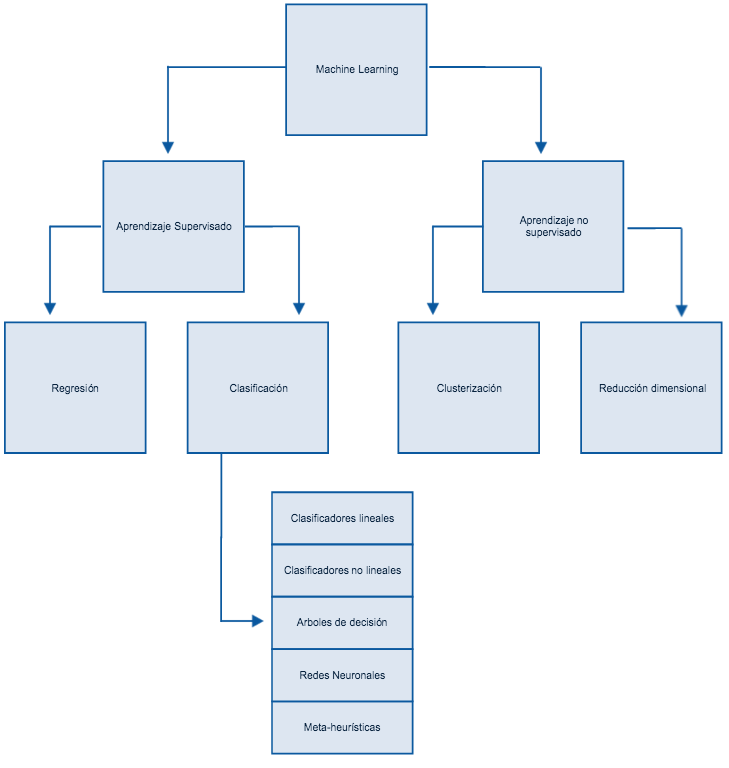
\includegraphics[width=1\textwidth]{Figures/Chapter1_Clasificacion}	
  \caption[Types of learning and the most common methods]
  {Distinct methods to solve problems in Machine Learning}
\end{figure}

\subsection{Fase de inferencia y fase de decisión}

Como primer paso, una vez elegido el método, se selecciona el criterio de penalización de los errores. Este debe ser elegido de manera acorde al problema planteado; por ejemplo, en el caso de una regresión lineal se desea que la penalización sea mayor en los datos que queden muy lejos del ajuste lineal, por lo que se escoge la norma euclidiana \footnote{Además de que las estimaciones hechas a través de mínimos cuadrados bajo ciertos supuestos tienen propiedades deseables de los estimadores: Que sean insesgados y de varianza mínima} $||x||_2 = \sqrt[]{x_{1}^{2}+x_{2}^{2}+ ... + x_{n}^{2}}$. En cambio, en un problema de clasificación se escoge una matriz de penalización o matriz de pérdida, en la que se establece el costo por cada tipo de error de clasificación.

Como segundo paso, se procede con la fase de inferencia, en la que se ajustan los estimadores de los parámetros del modelo elegido de acuerdo a los datos que se tienen, esto con el fin de hacer la inferencia de las distribuciones poblacionales. Como tercer y último paso, se procede a la fase de decisión, en la que se busca encontrar un criterio de decisión que minimice la pérdida esperada \cite{bishop2006pattern}. Por ejemplo, para los problemas de clasificación es muy claro determinar estas dos fases: la primera, se lleva a cabo al determinar la distribución conjunta de clases de pertenencia e individuos; mientras que la segunda, se realiza al determinar las fronteras de decisión basadas en estas probabilidades. Por otra parte, para los problemas de regresión tradicional, ambas fases se realizan al mismo tiempo, ya que al calcular los estimadores de los parámetros se utiliza el método de mínimos cuadrados que minimiza la penalización cuadrática.


\section{Clasificación con modelos lineales}


Se comenzará definiendo la nomenclatura utilizada en esta tesis. Las clases se denotan con la variable aleatoria $k \in C$, con $C  = \{ k = k_j: j = 1, \vdots, K\}$ el conjunto de posibles clases a clasificar y $n(C) = K$ la cardinalidad del conjunto. Para los individuos se define la variable aleatoria $x \in {\rm I\!R}^{m}$. De esta manera, sea $p(x, k)$ \footnote{Teniendo esta probabilidad se pueden calcular fácilmente las probabilidades condicionales $p(k|x)$ y $p(x|k)$} la distribución conjunta de individuos $x$ con clases $k$.


Para la fase de inferencia se utilizan los datos de entrenamiento, donde se distingue a los individuos y a sus clases de pertenencia $x_i \in  {\rm I\!R}^{m}$ y $y_i \in {\rm I\!R}$ respectivamente, con $i = 1, ... , N$. Agrupándolos en matrices, sea $X \in {\rm I\!R}^{N \times m}$ la matriz de individuos y $Y \in {\rm I\!R}^{N \times 1}$ el vector de clases de pertenencia asociada a cada individuo. Una vez hecha la inferencia, se pueden encontrar clases predichas para los individuos $x_i$, se denotará como $\widehat{y_i}$ y $\widehat{Y}$ a la respectiva matriz.


\begin{table}
\caption{Nomenclatura usada en el texto}
\begin{center}
    \begin{tabular}{ | l | c | c | p{4.5cm} |}
    \hline
    Tipo & Definición & Valores & Descripción  \\ \hline
    Entero & $K$ & $K \in \mathbb{N}$ & Número de posibles clases. \\ \hline
    Entero & $N$ & $N \in \mathbb{N}$ & Número de individuos en los datos. \\ \hline
    Entero & $N_k$ & $N_k \in \mathbb{N}$ & Número de individuos en la clase $k$. \\ \hline
    Entero & $m$ & $m \in \mathbb{N}$ & Dimensión de los individuos. \\ \hline
    v.a. & $k$ & $k \in C$ & Variable aleatoria de las clases. \\ \hline
	v.a. & $x$ & $K \in {\rm I\!R}^{m}$ & Variable aleatoria de los individuos. \\ \hline
    Conjunto & $C$ & $k_j: j = 1 ... K$ & Conjunto de posibles clases. \\ \hline
    Dato & $x_i$ & $x_i: i = 1 ... N$ & Vector columna del individuo $i$. \\ \hline
    Dato & $y_i$ & $y_i: i = 1 ... N$ & Dato de clase real del individuo $i$. \\ \hline
    Dato & $\widehat{y_i}$ & $\widehat{y_i}: i = 1 ... N$ & Dato de clase predicha del individuo $i$. \\ \hline
    Dato & $X$ & $X^T = [x_1 |...| x_N]$ & Matriz de individuos. \\ \hline
    Dato & $Y$ & $Y^T = [y_1 | ... | y_n]$ & Vector de clases reales de infividuos. \\ \hline
    Datos & $\widehat{Y}$ & $\widehat{Y}^T = [\widehat{y_1} | ... | \widehat{y_n}]$ & Vector de clases predichas de infividuos. \\ \hline
    Distribución & $p(x,k) $ &  & Distribución conjunta de individuos y clases \\ \hline
    \end{tabular}
\end{center}
\end{table}


\subsection{Fase de inferencia}
Como se mencionaba antes, en fase de inferencia se busca encontrar la distribución conjunta de la muestra con cada una de las clases, es decir $p(x,k)$. La dificultad en estimar esta distribución aumenta conforme la dimensionalidad de $x$ crece y conforme el número de clases aumenta \footnote{Para poder estimar la distribución conjunta, el número de clases debe ser menor que el conjunto de individuos}. Esto es debido a que se comienza a requerir un conjunto de datos mayor para poder estimar cada punto de $p(x,k)$. Por esta razón, muchas veces es suficiente encontrar directamente $p(k|x)$; es decir, dadas las características del individuo, encontrar que tan probable es que pertenezca a cada clase. Por otro lado, en la fase de decisión se encuentra la asignación óptima dependiendo de la matriz de pérdida que se seleccionó y de las probabilidades calculadas (ya sea la distribución conjunta o las condicionales). 

Los modelos propuestos para resolver la fase de inferencia se pueden agrupar de la siguiente manera \cite{bishop2006pattern}: 

\begin{enumerate}
	\item  \textbf{Modelos Probabilísticos Generativos.}
    Plantean resolver el problema de inferencia con el objetivo de determinar $p(x,k)$; es decir, la distribución conjunta de individuos y clases. Una vez obtenida la distribución, se puede usar para calcular $p(x|k)$, $p(k|x)$, $p(x)$ o $p(k)$. Para este enfoque se tienen que hacer supuestos acerca de la distribución de $x$ o $x|k$, o bien, tener un conjunto de entrenamiento muy grande que permita inferir acertadamente $p(x,k)$.

    Tomando propiedades básicas de probabilidad, se pueden calcular las distribuciones necesarias:
  
    \begin{equation} \label{eq:1}
     p(x, k) = p(x|k) p(k)
    \end{equation}

    \begin{equation} \label{eq:2}
     p(x, k) = p(k|x) p(x) 
    \end{equation}
    
    \begin{equation} \label{eq:3}
     p(k|x)  = \frac{p(x|k)p(k)}{p(x)}
    \end{equation}

	\begin{equation} \label{eq:4}
	 p(x) = \sum_{k} p(x|k)p(k) 
	\end{equation}
	
	\begin{equation} \label{eq:5}
	 p(k) = \sum_{x} p(k|x)p(x) 
	\end{equation}
	
	En caso de no tener suficientes datos para inferir directamente esta distribución; o bien, de no tener conocimiento de la estructura de la distribución de $x$, se dan preferencia a los modelos discriminativos o modelos de funciones discriminantes.

\textit{Ventajas\cite{bishop2006pattern}:}
\begin{itemize}
\item Puede ser útil para detectar datos atípicos, ya que al supone una distribución de $x$, se puede determinar qué puntos son poco probables de suceder. De esta manera, se puede encontrar qué predicciones podrían fallar. 
\end{itemize}

\textit{Desventajas\cite{bishop2006pattern}:}
\begin{itemize}
\item Se debe tener información acerca de la distribución de $x$.

\item Inferir directamente de los datos la distribución $p(x,k)$ puede ser muy demandante cuando la dimensionalidad de $x$ es alta. 

\item Si solo se requiere hacer clasificación, puede ser ineficiente encontrar toda la distribución conjunta.
\end{itemize}


\item \textbf{Modelos Probabilísticos Discriminativos.}
Primero, se resuelve el problema de inferencia para determinar $p(k|x)$ con los datos, y después se procede a la fase de decisión para asignar la clase de pertenencia.

\textit{Ventajas:\cite{bishop2006pattern}}
\begin{itemize}
\item Solo se necesita estimar $p(k|x)$ y no toda la distribución conjunta.
\end{itemize}

\textit{Desventajas:\cite{bishop2006pattern}}
\begin{itemize}
\item No se tiene la detección de atípicos presentados por el primer enfoque.
\end{itemize}


\item \textbf{Función Discriminante}
Plantea encontrar una función $\widehat{f}:{\rm I\!R}^m \rightarrow {\rm I\!R}$, tal que clasifique directamente a cada individuo en una clase $k$, de esta manera se define $\widehat{Y}=\widehat{f}(x)$. 

\textit{Ventajas:\cite{bishop2006pattern}}
\begin{itemize}
\item Se combina la fase de inferencia y la fase de decisión en una sola función $\widehat{Y}=\widehat{f}(x)$. 
\end{itemize}

\textit{Desventajas:\cite{bishop2006pattern}}
\begin{itemize}
\item Ya no se cuenta con las probabilidades posteriores $p(k|x)$, por lo que ya no se puede analizar una a una la probabilidad de pertenencia del individuo $x$ a cada una de las clases.
\end{itemize}

\end{enumerate}


\subsection{Fase de decisión}
Para la fase de decisión es conveniente analizar tres definiciones: ``Regiones de decisión'',  ``Fronteras de decisión'' y  ``Funciones discriminantes''. Las primeras dos reciben este nombre porque buscan dividir el espacio al que pertenecen los datos en regiones distintas y excluyentes. Cada una de estas regiones $R_{k}$ clasifica al individuo $x$ en una única clase $k$. En cambio, las fronteras de decisión son las zonas que delimitan una región de las demás; es decir, en ellas (o en sus cercanías) es indiferente qué clase elegir. Por esta razón, es conveniente analizar los datos que quedan cercanos para poder hacer una elección, tomando en cuenta la naturaleza del problema. Por último, las Funciones Discriminantes, nos permiten comparar directamente qué tan verosímil es que un individuo pertenezca a una clase u a otra.

Debido a la finalidad del texto se proponen fronteras lineales \footnote{Las fronteras de decisión pueden tomar formas irregulares, pero en general su forma depende del método de clasificación elegido}, ya que al igual que una regresión lineal, es la base que ejemplifica modelos más complejos. Por este motivo, se mostrarán distintas opciones para construir las regiones y fronteras que se adecuan a los tres enfoques distintos: modelos probabilísticos generativos, modelos probabilísticos discriminativos y funciones discriminantes. 

Para asegurar la linealidad en las fronteras, se debe hacer un análisis que garantice esta propiedad. Se ejemplificará con un caso de dos clases: $k_i$ y $k_j$ con $\left( \begin{array}{ccc}
0 & c_{ij} \\
c_{ji} & 0 \\
 \end{array} \right)$, la matriz de costos con $c_{ij}$ el costo de elegir $i$ cuando la verdadera clase es $j$. Se supone que $c_{ij}, c_{ji}$ mayores que 0. De esta manera la frontera de decisión está dada por:

\begin{equation} \label{eq:6}
c_{ij} p( k = k_i | x \in k_j) - c_{ji} p(k = k_j| x \in k_i) = 0
\end{equation}

De otra manera, si $c_{ij} p( k = k_i | x \in k_j) < c_{ji} p( k = k_j| x \in k_i) $ o viceversa, entonces se clasificará hacia $k_i$ y $k_j$, respectivamente. Para los fines de esta tesis, se tomarán los costos de $c_{ij} = c_{ji} = 1$ ya que esto solo juega en la ordenada al origen de la ecuación de la frontera lineal. Tomando un resultado presentado por T. Mitchell \cite{mitchell2006discipline}, si se aplica una función monótona de $p(k, x)$, la linealidad de las fronteras de decisión se mantiene. En este caso, se toma la función de logaritmo $log()$:


$$ log(p(k = k_j | x)) = log( p(k = k_i | x)) $$	

\begin{equation} \label{eq:7}
 log \frac{p( k = k_j | x )}{ p(k =  k_i |  x)} = 0 	
\end{equation}

El lado izquierdo de esta última ecuación es conocido como razón de momios (log odd). Cuando es una función lineal con respecto a $x$, mantiene la linealidad de la frontera:

\begin{equation} \label{eq:8}
 log \frac{p(k = k_j | x )}{p(k = k_i |  x)} = \beta_0 + x^T \beta_1 
\end{equation}


\section{Métodos de clasificación lineales}

En la fase de inferencia se busca construir la distribución $p(x,k)$, la cual será usada en la fase de decisión para tomar un criterio óptimo de clasificación. En la sección 2.2 se mostraron los distintos enfoques que se toman para hacer esta inferencia. Recapitulando, para modelos generativos se escoge $\widehat{Y}(x) = \widehat{f}(p(x,k))$; para modelos discriminativos $\widehat{Y}(x) = \widehat{f}(p(k|x))$ y para funciones discriminantes se escoge $\widehat{Y}(x)$ = $\widehat{f}(x)$. En los dos primeros casos se ve que la función $f$ toma como entrada distribuciones concernientes a $x$ y $k$, pero en el tercer caso, solamente toma como entrada a $x$. En esta sección se ejemplificarán los 3 métodos con técnicas sencillas. Para el enfoque Probabilístico Generativo se empleará el Análisis Discriminante Lineal, para el Probabilístico Discriminativo la Regresión Logística y para la función discriminante, el Discriminante Lineal de Fisher.

En los siguientes tres ejemplos se explica cómo se realiza la inferencia de las distribuciones, para después demostrar la linealidad en las fronteras. Como se explica en la sección 2.2.2, si se asegura que (\ref{eq:8}) es lineal con respecto a $x$, entonces se garantiza la linealidad de estas. En la Regresión Logística se ejemplificará el procedimiento para $n$ clases. Para los demás se supondrá el caso de la frontera entre dos clases.


\subsection{Modelos discriminativos: Regresión Logística}


\textit{Inferencia de la distribución $p(k | x)$} \\
Para la fase de inferencia, se calculan las probabilidades posteriores de pertenecer a cada grupo $j$, de manera que: 
\begin{equation} \label{eq:15}
	\sum\limits_{j = 1}^{K} p(k = k_j | x) = 1
\end{equation}


\textit{Linealidad de la frontera}\\
Para obtener la estimación de las $K$ distribuciones de probabilidad $p(k = k_j | x)$, se parte de la ecuación (\ref{eq:8}) y se supone que todas las fronteras son lineales.

$$ \log \frac{p(k = k_1 | x)}{p(k = k_K | x)} = \beta_{1.0} + \beta_1^T x$$

$$ \log \frac{p(k = k_2 | x)}{p(k = k_K | x)} = \beta_{2.0} + \beta_2^T x$$

$$\vdots$$

$$ \log \frac{p(k = K-1 | x)}{p(k = k_K | x)} = \beta_{(K-1).0} + \beta_{(K-1)}^T x$$

Con estas ecuaciones se crea un sistema que cuenta con $K$ variables $p(k = k_j| x)$ y $K-1$ ecuaciones, lo cual, añadiendo la restricción (\ref{eq:15}) se puede despejar cada probabilidad: 

$$ p(k = k_1 | X = x) = \frac{\exp(\beta_{1.0} + \beta_1^T x)}{1+\sum\limits_{i=1}^{K-1} {\exp(\beta_{l.0} + \beta_l^T x)}} $$

$$ p(k = k_2 | X = x) = \frac{\exp(\beta_{2.0} + \beta_2^T x)}{1+\sum\limits_{i=1}^{K-1} {\exp(\beta_{l.0} + \beta_l^T x)}} $$

$$ \vdots $$

$$ p(k = k_{K-1} | X = x) = \frac{\exp(\beta_{(K-1).0} + \beta_{(K-1)}^T x)}{1+\sum\limits_{i=1}^{K-1} {\exp(\beta_{l.0} + \beta_l^T x)}} $$

Para la clase de referencia: 

$$ p(Y = k_K | X = x) = \frac{1}{1+\sum\limits_{i=1}^{K-1} {\exp(\beta_{l.0} + \beta_l^T x)}} $$

Para tener la formulación completa, falta estimar las $\beta$ de cada probabilidad. Esto, comúnmente, se realiza con máxima verosimilitud (a través de métodos iterativos como Newton) \cite{hastie2009elements}


\textit{Funciones $logit$ y $logit^{-1}$} \\
Para este modelo es conveniente analizar la función logit y su inversa:
 
 \begin{equation} \label{eq:16}
 logit = \log (\frac{p}{1-p}) 
 \end{equation}

\begin{equation} \label{eq:17}
 logit^{-1}  = \frac{\exp(x)}{1+\exp(x)}
 \end{equation}


Al graficar la función $logit$ y la $logit^{-1}$ sobre un plano (Figura 1.1) se observan algunas de sus propiedades. En la gráfica de la izquierda, se realiza un mapeo de valores del rango (0,1) al rango (-$\inf$,$\inf$), mientras que a la derecha se transforman valores continuos de (-$\inf$, $\inf$) al $(0,1)$. La transformación realizada por $logit^{-1}$ es de mayor interés ya que su rango es semejante al que toman las probabilidades. Este enfoque nos da una amplia gama de elección para la fase de decisión, ya que deja elegir los puntos de corte para cada clase, dependiendo la penalización que se quiera dar a cada tipo de error \cite{hastie2009elements}:

\begin{figure}[!ht]
  \centering
	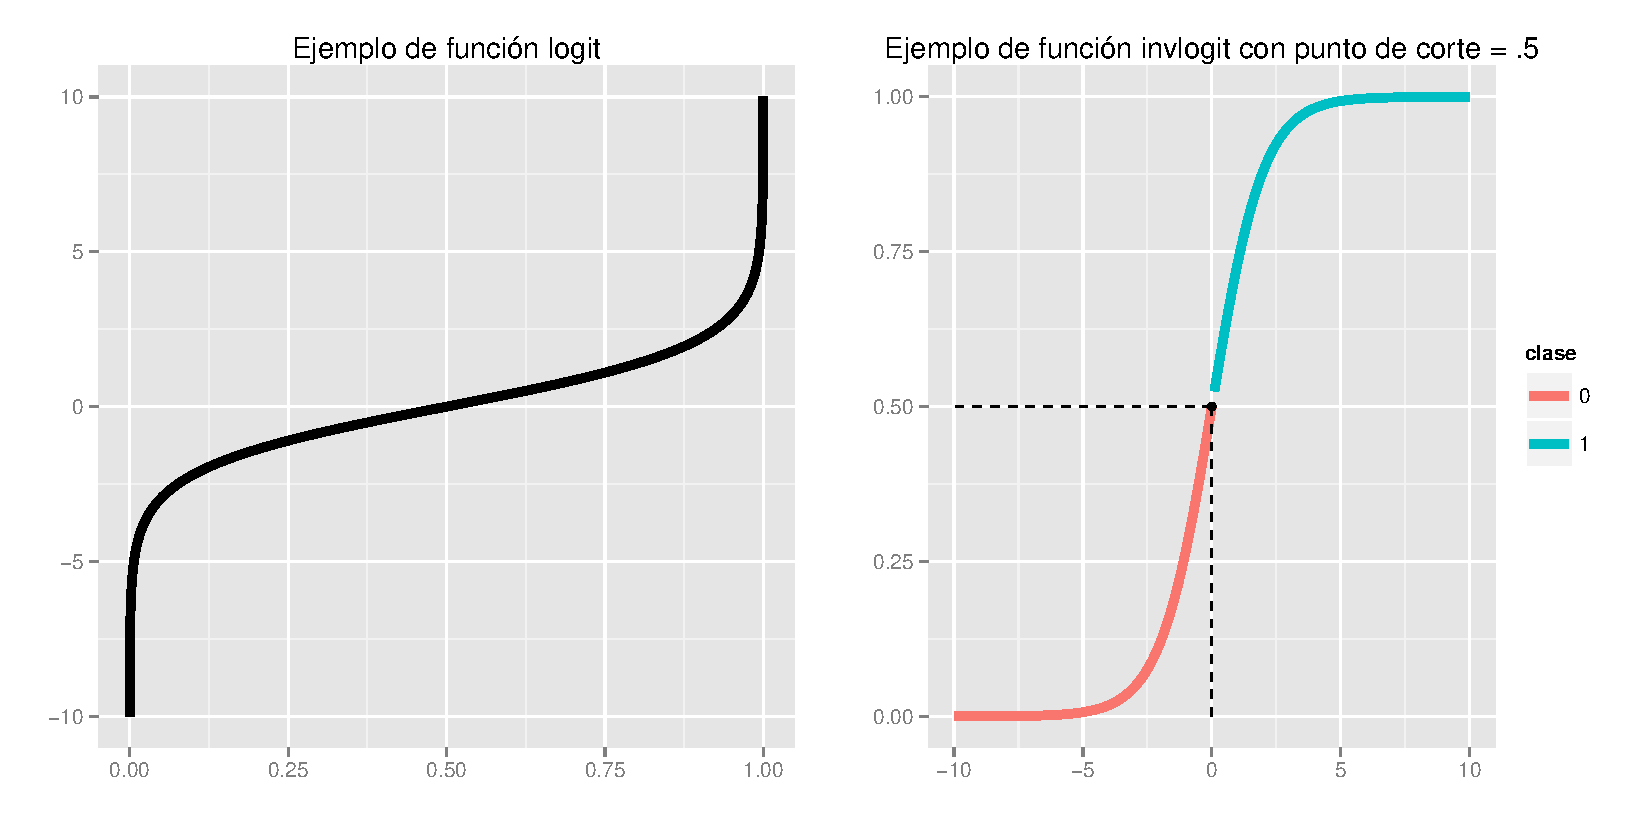
\includegraphics[width=1\textwidth]{Figures/Chapter1_logit}	
  \caption[Función logit y $logit^{-1}$]
  {En la izquierda se muestra la función logit y en la derecha la función $logit^{-1}$ con punto de corte p = .5; es decir, se escoge la clase 1 en la zona azul y la clase 0 en la zona roja.}
\end{figure}

\pagebreak
\subsection{Modelos generativos: Análisis Discriminante Lineal}


\textit{Inferencia de la distribución $p(x,k)$}\\
Para el caso del Análisis Discriminante Lineal se sigue un enfoque generativo, en el que se realiza inferencia de $p(x,k)$. Primero, se supondrá que $p(x|k)$ sigue una distribución Gaussiana con varianza $\Sigma_{k}$ constante para todas las clases y $\mu_{k}$ la media de los individuos pertenecientes a la clase $k$ (ecuación (\ref{eq:9})). Por otra parte, se estima la distribución $p(k)$ como la proporción de casos que cada clase aparece en los datos (ecuación (\ref{eq:10})). Usando la ecuación (\ref{eq:1}) se deduce $p(x,k)$:


\begin{equation} \label{eq:9}
 p(x|k) = \frac{1}{(2\pi) |\Sigma|^{1/2}} e^{-\frac{1}{2}(x-\mu_{k})^{T}\Sigma^{-1}(x-\mu_{k})}
\end{equation}

\begin{equation} \label{eq:10}
 p(k) = \frac{N_k}{N}	
\end{equation}

Por otro lado, al utilizar el Teorema de Bayes (\ref{eq:3}) y la ecuación (\ref{eq:4}), se puede calcular $p(k|x)$ directamente. 



\textit{Linealidad de la frontera}\\
Al hablar de la linealidad de la frontera, se tiene que cumplir la ecuación (\ref{eq:8}), enunciada en la sección 2.2.2:

$$\log \frac{p(k = k_j | x )}{p(k = k_i |  x)} = \beta_0 +  x^T \beta_1$$

$$\log \frac{p(x | k = k_j)p(k = k_j)}{p( x | k = k_i)p(k = k_i)} = \beta_0 +  x^T \beta_1$$

\begin{equation} \label{eq:11}
 	\log\frac{p(x | k = k_j)}{p(x | k = k_i)} + \log\frac{p(k = k_j)}{p(k = k_i)} = \beta_0 +  x^T \beta_1
\end{equation} 

La ecuación (\ref{eq:11}) consta de dos sumandos. Al desarrollar el primero:

$$ \log\frac{p(x | k = k_j)}{p(x | k = k_i)} = -\frac{1}{2}[(x - \mu_j)^T \Sigma^{-1}(x - \mu_j) - (x - \mu_i)^T \Sigma^{-1}(x - \mu_i)] $$ 


\begin{equation}
\begin{aligned}
 \log\frac{p(x | k = k_j)}{p(x | k = k_i)} =& -\frac{1}{2}[{\mu_j}^T \Sigma^{-1} {\mu_j}  -  {\mu_i}^T \Sigma^{-1} {\mu_i}]  + \\
 &\frac{1}{2}[{x}^T \Sigma^{-1}(\mu_j-\mu_i) - {(\mu_j-\mu_i)}^T \Sigma^{-1}(x)
\end{aligned}
\end{equation}

 

 \begin{equation} \label{eq:12}
 	\log\frac{p(x| k = k_j)}{p(x | k = k_i)} = -\frac{1}{2}[{(\mu_j - \mu_i)}^T \Sigma^{-1} {(\mu_j + \mu_i)}] + [{x}^T \Sigma^{-1}(\mu_j-\mu_i)]
 \end{equation}

Sustituyendo \ref{eq:12} en \ref{eq:11} se tiene como resultado:

$$ \log \frac{p(k = k_j)}{p(k = k_i)} - \frac{1}{2}[(\mu_j - \mu_i)^T \Sigma^{-1} (\mu_j + \mu_i)] + {x}^T \Sigma^{-1} (\mu_j - \mu_i) = \beta_0 +  x^T \beta_1$$

Del cual se nota que $\beta_0$ y $\beta_1$ son equivalentes a:

\begin{equation} \label{eq:13}
\beta_0 = \log \frac{p(k = k_j)}{p(k = k_i)} - \frac{1}{2}[(\mu_j - \mu_i)^T \Sigma^{-1} (\mu_j +\mu_i)] 	
\end{equation}

\begin{equation} \label{eq:14}
 \beta_1 = \Sigma^{-1} (\mu_j -\mu_i)
\end{equation}


\textit{Funciones Discriminantes} \\
Ahora, solo falta enunciar las funciones discriminantes de la clase $i$ y $j$; es decir, $log p(k = k_i | x)$ y  $log p(k = k_j | x)$, respectivamente:
$$ \delta_j (x) = \log {p(k = k_j)} - \frac{1}{2}\mu_j^T \Sigma \mu_j + x^T \Sigma^{-1} \mu_j$$
$$ \delta_i (x) = \log {p(k= k_i)} - \frac{1}{2}\mu_i^T \Sigma \mu_i + x^T \Sigma^{-1} \mu_i$$


\subsection{Funciones Discriminantes: Discriminante Lineal de Fisher}

El Discriminante Lineal de Fisher es similar al Análisis Discriminante Lineal. El primero permite ver una proyección informativa en un espacio de dimensión menor \cite{hastie2009elements}. Este planteamiento fue propuesto por Fisher \cite{fisher1936use}, y hace referencia a un discriminante lineal con menos supuestos \footnote{No toma en cuenta la distribución de los datos, ni la igualdad de varianzas entre las clases.}. Propone los supuestos de definir una varianza entre clases que es la varianza de las medias de las clases, y una varianza intra-clase, que mide la varianza dentro de las clases con respecto a la media de cada clase. Después, se busca una matriz de proyección $V$ que maximice la dispersión entre-clase al mismo tiempo que minimiza la dispersión intra-clase \cite{ngo2012trace}.

Se comenzará definiendo la nomenclatura necesaria para la sección. Sea $N_{k}$ el número de personas en la clase $k$, $N$ el número total de personas y $w_i = V^T x_i$; es decir, los datos proyectados con la matriz $V$. Entonces, se definen las medias de grupo $k$ como $\mu_k$ y la media de todos los datos $x_i$ como $\mu$:

\begin{equation} \label{eq:18}
 	\mu_k = \frac{1}{N_{k}} 
 	\sum_{\substack{i = 1\\
                  	y_i = k}}^{N}
                  x_i
\end{equation} 


\begin{equation} \label{eq:19}
 \mu = \frac{1}{N} \sum_{i = 1}^{N} x_i
\end{equation}

Por otro lado, se definen las medias correspondientes a los datos proyectados $w_i$:
\begin{equation} \label{eq:20}
 	\widetilde{\mu_k} = \frac{1}{N_{k}} 
 	\sum_{\substack{i = 1\\
                  	y_i = k}}^{N}
                  w_i
\end{equation} 


\begin{equation} \label{eq:21}
 \widetilde{\mu} = \frac{1}{N} \sum_{i = 1}^{N} w_i
\end{equation}


La matriz de dispersión intra-clase de los datos proyectados:


$$\Phi_{I} = \sum_{k=1}^{K} 
				\sum_{\substack{i = 1\\
                  			   	y_i = k}}
                    ^{N}
           ||w_i-\widetilde{\mu}_{k}||^{2}_{2}$$


$$ \Phi_{I} =  \sum_{k=1}^{K} 
					\sum_{\substack{i = 1\\
                  			   	y_i = k}}
                    ^{N}
			Tr (V^T (x_i - \mu_k)(x_i - \mu_k)^T V ) $$

\begin{equation} \label{eq:22}
 \Phi_{I} =  Tr(V^T S_I V) 
\end{equation}



\begin{equation} \label{eq:23}
con \quad S_I = \sum_{k=1}^{K} 
					\sum_{\substack{i = 1\\
                  			   	y_i = k}}
                    ^{N}
 ({x_i-\mu_{k}})({x_i-\mu_{k}})^T 
\end{equation}



La matriz de dispersión entre-clases de los datos proyectados:

$$ \Phi_{E} = \sum_{k=1}^{K} N_{k} || \widetilde{\mu}_k - \widetilde{\mu} ||^{2}_{2} $$

$$ \Phi_{E} = \sum_{k=1}^{K} N_{k} || V^T \mu_k - V^T \mu ||^{2}_{2} $$
 
$$ \Phi_{E} =  \sum_{k=1}^{K} N_{k} V^T(\mu_k - \mu)(\mu_k - \mu)^T V $$
\begin{equation} \label{eq:24}
 \Phi_{E} =  Tr(V^T S_E V)  
\end{equation}

\begin{equation} \label{eq:25}
 con \quad S_E = \sum_{k=1}^{K} N_{k} (\mu_k - \mu)(\mu_k - \mu)^T 
\end{equation}

De este modo, se definen las dos matrices importantes del método: $S_I$ la matriz de dispersión interna y $S_E$ la matriz de dispersión entre clases. Con estas definiciones surge la idea intuitiva de maximizar $\Phi_{E}$ al mismo tiempo que se minimiza $\Phi_{I}$; es decir, encontrar un espacio de proyección en el que los grupos pertenecientes a la misma clase tengan poca varianza, al mismo tiempo que la varianza entre estas clases sea alta. Se puede plantear esta idea a través del problema de maximización:

\begin{equation}\label{eq:26}
	\max_{\substack{V \in {\rm I\!R}^{n\times p} \\ V^TV = I}} \frac{Tr(V^T S_E V)}{Tr(V^T S_I V)} 
\end{equation}

Este problema de optimización es el principal tema de la tesis, por lo que los detalles acerca de las fronteras y el proceso de maximización que derivan en encontrar la matriz óptima $V$ será analizado en los capítulos siguientes.

\section{Enfoques para la minimización del error}

La teoría de la decisión se aplica para la fase dos, en la que se busca tomar decisiones óptimas dadas las probabilidades calculadas en la fase de inferencia. La motivación de una teoría de la decisión es que las probabilidades, por sí solas, no nos indican que clase elegir, solamente nos dan información del comportamiento de la distribución. Por esta razón, es conveniente saber que decisión tomar basándonos en la penalización de los errores elegidos anteriormente. Puede verse desde dos perspectivas \footnote{En realidad el primer enfoque es un caso particular del segundo}:

\begin{itemize}
\item Minimizar el error de clasificación a lo largo de todos nuestros datos.
\item Minimizar la pérdida esperada dada una matriz de pérdida L. 
\end{itemize}


\subsection{Minimizando el error de clasificación}
Esta regla dividirá el espacio en regiones $R_j$ en las que cada individuo es asignado a una clase $k_j$ con $j = 1, ... , K$. Recordando la nomenclatura, $x_i$ es el individuo $i$ y $y_i$ es la clase a la que pertenece este sujeto; mientras que $\widehat{y}_i$ es la clase predicha del sujeto $i$. Por otro lado, $k_j$ es la clase $j$ de las $K$ existentes. Para encontrar la decisión óptima de elección se busca minimizar la probabilidad de cometer errores, que está dada por:

%$$p(error) = 1 - \sum_{i = 1}^{N} \sum_{j=1}^{K} p(y_i = k_j, \widehat{y}_i = k_j)$$


$$p(error) = 1 - \sum_{i = 1}^{N} \sum_{j=1}^{K} p(x_i \in R_{j}, y_i = k_j)$$

En la expresión anterior, cuando $x_i \in R_j$ se sabe que $\widehat{y}_i$ esta asociada a la clase $k_j$. Ocupando la igualdad $p(x \in R_{j}) = \int_{R_j} p(x) dx$ se tiene que es equivalente a maximizar la probabilidad de no cometer errores:

$$p(no error) = \sum_{i = 1}^{N} \sum_{j=1}^{K} p(x_i \in R_{j},  y_i = k_j)$$

$$p(no error) = \sum_{i = 1}^{N} \sum_{j=1}^{K} \int_{R_j} p(x_i, y_i = k_j) dx $$

Es facil deducir que $\int_{R_j} p(x_i, y_i = k_j) dx$ es equivalente a que $p(\widehat{y}_i = k_j, y_i = k_j)$ porque cuando $x_i$ está en la región $R_j$, entonces $\widehat{y}_i = k_j$. Ocupando esta igualdad se puede deducir:

\begin{equation}\label{eq:27}
p(no error) = \sum_{i = 1}^{N} \sum_{j=1}^{K} p(\widehat{y}_i = k_j, y_i = k_j) 
\end{equation}

Es decir, dado que $x_i$ pertenece a la región $R_{j}$ (y por lo tanto es clasificado en la clase $k_j$) y la clase original de $x_i$ es $y = k_j$, implica que la clasificación es correcta. La maximización de (\ref{eq:27}) sigue un argumento intuitivo. Al obtener la distribución $p(x, k)$, se selecciona aquella que tiene la probabilidad más alta de ocurrir para cada individuo; es decir, tomar como criterio de decisión la que tenga mayor $p(x_i \in R_j)$. 

En los Modelos Probabilísticos Generativos se utiliza la distribución conjunta, en cambio en los discriminativos solamente se utiliza $p(k|x)$. Para extender el resultado anterior a la distribución condicional se ocupa la ecuación $\ref{eq:2}$:

$$p(x,k)  = p(k|x)p(x)$$

Maximizar $p(x,k)$ es equivalente a maximizar el término de la derecha. Como $p(x)$ es positivo y común a todos los términos, es equivalente a seleccionar la clase con probabilidad $p(k|x)$ más grande para cada individuo. 

\subsection{Minimizando la pérdida esperada}

Tomando una matriz de pérdida se puede ver más general el error de clasificación. La motivación de este enfoque es la disparidad en los distintos costos asociados a cada tipo de error de clasificación. Por ejemplo, en un problema en el que se predice si a un paciente le dará un ataque al corazón, es peor predecir que no tendrá un ataque cuando en realidad si lo tendrá \cite{hastie2009elements}. Por esta razón, la modelación del error a través de una matriz de pérdida tiene sentido. Sea $L$ la matriz que tiene como característica el tener ceros en la diagonal y pesos no negativos en cualquier otro lado y $L(X,Y)$ el costo asociado a elegir Y cuando la clase verdadera es X. \footnote{Es fácil notar que la matriz $L_{0-1}$; es decir, 0 sobre la diagonal (Clasificación correcta) y 1 (Clasificación incorrecta) en cualquier otro lugar, es equivalente al enfoque que minimiza el error de clasificación}

Tomando el error esperado de predicción de los vectores $Y$ y $\widehat{Y}$ bajo la matriz $L$:

$$ EEP = E[L(Y, \widehat{Y})] $$

En la que $Y$ es el vector de clases de pertenencia verdaderas y $\widehat{Y}$ es el vector de clases de pertenencias predichas. Ambos vectores son de variables categóricas que pueden tomar valores $k_j \in C$ con $j = 1 ... K$. 

Al desarrollar el error esperado de predicción como una sumatoria sobre los $N$ individuos y las $K$ clases, es equivalente a:

$$EEP = \sum_{i = 1}^{N} \sum_{j=1}^{K} L[y_i = k_j, \widehat{y}_i = k_j] p(x = x_i, k = k_j)$$

Sustituyendo $p(k, x) = p(k | x)p(x)$, se puede calcular la esperanza sobre los individuos $x$. Lo que se deduce la expresión:

$$EEP = E_{x} \sum_{j=1}^{K} L[y = k_j, \widehat{y} = k_j] p(k_j | x)$$

Como se busca minimizar el error esperado de predicción con respecto a $\widehat{y}$, se obtiene el siguiente problema de minimización:

$$\widehat{y}^{*} = \argmin_{\widehat{y}} E_{x} \sum_{j=1}^{K} L[y = k_j, \widehat{y} = k_j] p(k_j | x)$$

Este problema de minimización es equivalente a minimizar el error esperado de predicción para cada individuo $x$:

$$\widehat{y}^{*} = \argmin_{\widehat{y}} \sum_{j=1}^K L[y = k_j, \widehat{y} = k_j]p(k_j|x)$$

Al escoger la función de pérdida $0-1$, cuando $\widehat{y}^{*} = y$, entonces la pérdida es igual a 0, por lo que la fórmula se simplifica a:

$$\widehat{y}^{*} = \argmin_{\widehat{y}}
\sum_{\substack{j = 1 \\
			   y \neq \widehat{y}}} ^ K 
			   L[y = k_j, \widehat{y} = k_j] p(k_j | x)$$

Por otro lado, cuando $\widehat{y}^{*} \neq y$ entonces la pérdida es igual a 1:

$$\widehat{y}^{*} = \argmin_{\widehat{y}}
\sum_{\substack{j=1 \\
      y \neq \widehat{y}}}^K
p(k_j | x)$$

$$\widehat{y}^{*} = \argmin_{\widehat{y}} 
[1 - \sum_{\substack{j=1 \\
      y = \widehat{y}}}^K
p(k_j|x)]$$

Esta expresión es equivalente a maximizar:

$$\widehat{y}^{*} = \argmax_{\widehat{y}} p(k|x)$$

De esta manera, se escoge $\widehat{y}^{*}$ como la probabilidad posterior más grande de pertenencia a la clase $k$ dado $x$. Esta solución es conocida como ``Clasificador de Bayes'' y nos dice que hay que clasificar a las clases más probables usando la distribución condicional $p(k|x)$. La tasa de error de este clasificador se le conoce como ``Tasa de Bayes''\cite{hastie2009elements}.



 
	%   \chapter{Discriminante Lineal de Fisher}
\label{ch:chapter2}

En este capítulo se hablará del Análisis Discriminante Lineal de Fisher (ADLF), el cual busca optimizar un cociente de la forma $Tr(V^T A V) / Tr(V^T B V)$ sobre el conjunto de matrices ortogonales $V$ con $A, B$ matrices positivas definidas. Para resolver el ADLF, se han presentado en libros de aprendizaje estadístico y clasificación de patrones formulaciones alternas al problema original, ya que este era considerado computacionalmente muy costoso \cite{wang2007trace}\cite{ngo2012trace}. Planteamientos como: maximizar la traza de la matriz de dispersión entre clases sujeto a una restricción sobre la matriz de dispersión interna, maximizar la traza del cociente de matrices; o bien, maximizar el cociente de determinantes, han sido formulaciones presentadas en distintos textos \cite{duda2012pattern} \cite{hastie2009elements} \cite{mitchell2006discipline} \cite{fukunaga2013introduction}. Al final, todas estas propuestas resultan ser versiones simplificadas del problema.

En este capítulo se resolverá el problema original del ADLF a través del método de Newton-Lanczos, el cual resulta ser computacionalmente eficiente. En la primer sección del capítulo se contextualizará al problema dentro del área de Aprendizaje de Máquina. En la segunda parte, se proporcionará la teoría correspondiente para seguir con facilidad el texto. Por último, en la tercera parte, se plantea la solución al problema de ADLF para una dimensión, se generaliza a $p$ dimensiones y se proporcionan las condiciones para la existencia de la solución.


\section{Aprendizaje de máquina}
El Aprendizaje de Máquina toma como base dos áreas de investigación: la Ciencia de la Computación y la Estadística. De la primera, retoma las preguntas: ¿Cómo se pueden construir máquinas que resuelvan problemas? Y ¿Qué problemas son tratables o intratables? De la segunda, toma las preguntas: ¿Qué puede ser inferido de los datos? ¿Bajo que supuestos del modelo? Y ¿Con qué confiabilidad? \cite{mitchell2006discipline}. El esfuerzo por resolver estas preguntas da como resultado una disciplina enfocada a construir teorías estadístico-computacional de los procesos de aprendizaje.

\subsection{Procesos de aprendizaje}

Se dice que una máquina ``aprende" dada una tarea (T), una medición del rendimiento (R) y un tipo de experiencia (E) si el sistema mejora confiablemente su rendimiento (R) en la tarea (T) dada la experiencia (E) \cite{mitchell2006discipline}. Es decir, se modela una estructura con los datos proporcionados de manera que el rendimiento en la tarea mejora conforme más información recibe. La diversidad de las tareas, así como el campo de aplicaciones es muy diverso, por ejemplo:

\begin{itemize} 

\item \textit{Clasificación de spam/no-spam}, en el que (E) son los correos, (T) el clasificar correctamente el \textit{spam} y (R) el porcentaje de correos correctamente clasificados.

\item \textit{Reconocimiento/Clasificación facial}, en el que (E) son los rostros de distintas personas, (T) el reconocimiento o clasificación de los rostros y (R) el porcentaje de rostros correctamente reconocidos o clasificados.
\end{itemize} 

Los procesos de aprendizaje tienen diversas aplicaciones y distintos supuestos, por lo que han surgido clasificaciones para analizarlos en conjunto. La utilizada en este texto es la propuesta por T. Hastie \cite{hastie2009elements}, la cual divide a los métodos en dos grupos: aprendizaje supervisado y aprendizaje no supervisado. El primero, supone la presencia de una variable de salida que actúa como guía en la construcción de la estructura. Ejemplos de éste es la regresión lineal, los árboles de decisión y las máquinas de soporte vectorial. 
Por otra parte, el aprendizaje no supervisado solo cuenta con la información de las variables independientes; por ejemplo, análisis de conglomerados, reglas de asociación y reducción dimensional. 

Después de esta primer clasificación, se subclasifica a los métodos de aprendizaje supervisado de acuerdo al tipo de variable de salida (Figura 1.1). \footnote{A lo largo del texto se usará indiferentemente variable de entrada como ``input'' o variable independiente y variable de salida como ``output'' o variable dependiente} Cuando se trata de una variable cuantitativa recibe el nombre de regresión, mientras que en el caso de cualitativas se le llama clasificación. Por otra parte, el aprendizaje no supervisado tiene dos ramas en las que el texto hace énfasis \cite{hastie2009elements}: Segmentación en el caso que se desee asignar un grupo a cada individuo, de manera que los grupos sean homogéneos entre sí; o bien, reducción dimensional cuando solamente se desea proyectar a los individuos en un espacio de menor dimensión, de manera que se cumplan características especiales en dicho subespacio. 

El problema de ADLF pertenece a la rama de aprendizaje supervisado, en particular a los métodos clasificación. Alternativas para esta finalidad, y que sigan asumiento linealidad en la frontera, son la Regresión Logística, el Análisis Discriminante Lineal y las Máquinas de Soporte Vectorial. 

\begin{figure}[!ht]
  \centering
  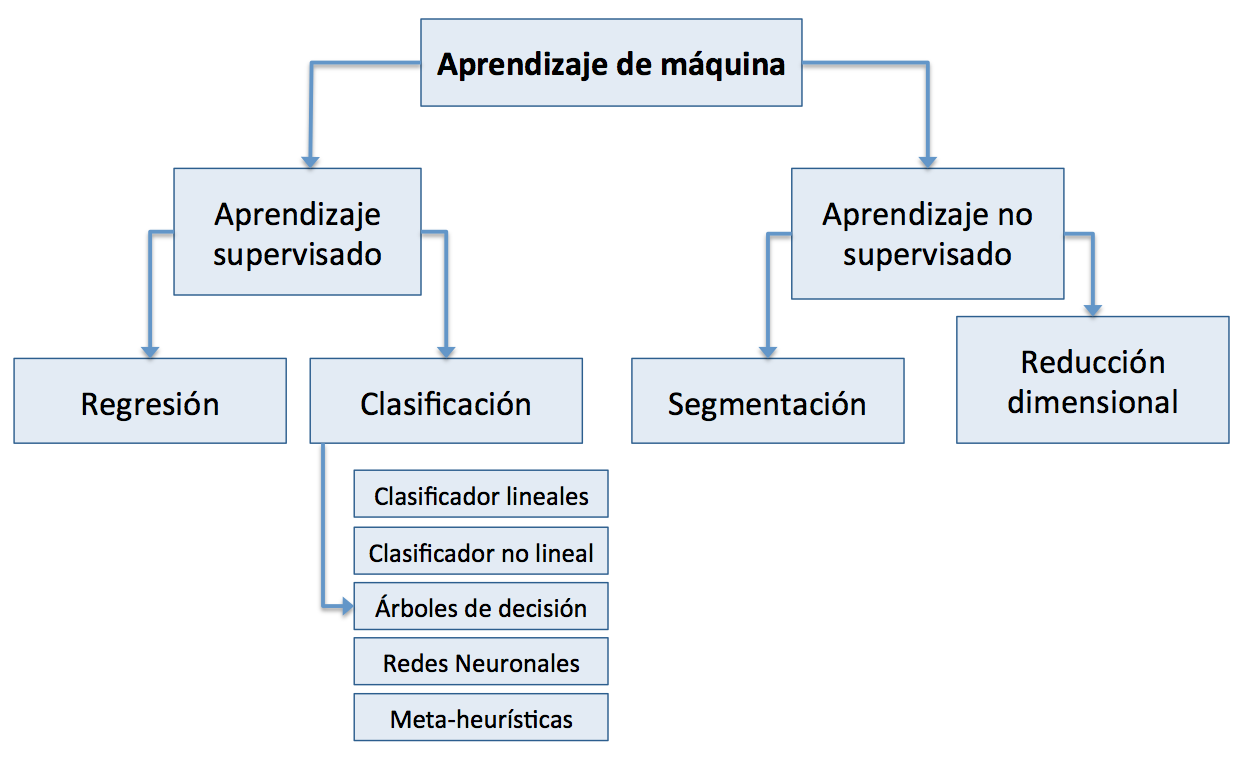
\includegraphics[width=1\textwidth]{Figures/Chapter1_Clasificacion1.png} 
  \caption[Enfoques para resolver problemas de clasificación.]
  {Distintos enfoques para resolver problemas de clasificación en el área de Aprendizaje de Máquina.}
\end{figure}

\section{Matrices de dispersión}
Se comenzará definiendo la nomenclatura necesaria para la sección. Sea $x_i$ el individuo $i$ que pertenece a la clase $y_i$, $N_{k}$ el número de personas en la clase $k$, $N$ el número total de personas y $w_i = V^T x_i$; es decir, los datos proyectados con la matriz $V$. Entonces, se definen las medias de grupo $k$ como $\mu_k$ y la media de todos los datos $x_i$ como $\mu$:

\begin{equation} \label{eq:18}
  \mu_k = \frac{1}{N_{k}} 
  \sum_{\substack{i = 1\\
                    y_i = k}}^{N}
                  x_i
\end{equation} 

\begin{equation} \label{eq:19}
 \mu = \frac{1}{N} \sum_{i = 1}^{N} x_i
\end{equation}

Por otro lado, se definen las medias correspondientes a los datos proyectados $w_i$:
\begin{equation} \label{eq:20}
  \widetilde{\mu_k} = \frac{1}{N_{k}} 
  \sum_{\substack{i = 1\\
                    y_i = k}}^{N}
                  w_i
\end{equation} 

\begin{equation} \label{eq:21}
 \widetilde{\mu} = \frac{1}{N} \sum_{i = 1}^{N} w_i
\end{equation}

El ADLF hace amplio uso de las matrices de dispersión, en específico de la matriz de covarianza, la matriz de dispersión de todos los individuos, la matriz de dispersión interna y la matriz de dispersión entre clases. Es importante analizar a profundidad la terminología y las fórmulas que se usarán a lo largo de la tesis para entender la lógica detrás de la formulación.

Sea $\Sigma$ la matriz de covarianza (\textit{Covariance Matrix)} de todos los individuos. Se define como $\widehat{\Sigma}$ al estimador insesgado de $\Sigma$ el cual está escalada entre $N-1$:

\begin{equation} \label{eq:2.1}
\widehat{\Sigma} = \frac{1}{N-1} \sum_{i=1}^{N}(x_i - \mu)(x_i - \mu)^T	
\end{equation}

Si esta matriz no está escalada por $N-1$ entonces se le conoce como matriz de dispersión (\textit{Scatter Matrix}), en esta tesis se representará como $S_T$, con el subíndice $T$ que significa que está tomando en cuenta a todos los individuos:

\begin{equation} \label{eq:2.2}
S_T = \sum_{i=1}^{N}(x_i - \mu)(x_i - \mu)^T	
\end{equation}

Cuando solo se toman a los individuos de una clase particular $k$, se puede encontrar su correspondiente matriz de dispersión, representada como $S_k$, con el subíndice $k$ simbolizando que está tomando en cuenta solo a los individuos de la clase $k$:

\begin{equation*}
S_k = \sum_{\substack{i=1 \\ y_i = k}}^{N} (x_k - \mu)(x_k - \mu)^T	
\end{equation*}

De esta manera se define la matriz de dispersión interna (\textit{Within-class scatter matrix}) como la suma sobre $k$ de todas las matrices de dispersión de cada clase:

\begin{equation}\label{eq:2.3}
S_I = \sum_{k=1}^{K} 
					\sum_{\substack{i = 1\\
                  			   	y_i = k}}
                    ^{N}
 ({x_i-\mu_{k}})({x_i-\mu_{k}})^T 	
\end{equation}

Ahora solo falta definir la matriz de dispersión entre clases (\textit{Between-class scatter matrix}) como la suma de diferencias al cuadrado de las medias de clase contra la media de todos los datos multiplicada por el número de individuos en cada clase $N_k$:

\begin{equation} \label{eq:2.4}
S_E = \sum_{k = 1}^K N_k (\mu_k - \mu)(\mu_k - \mu)^T	
\end{equation}

\begin{figure}[!ht] \label{Fig1.1}
  \centering
	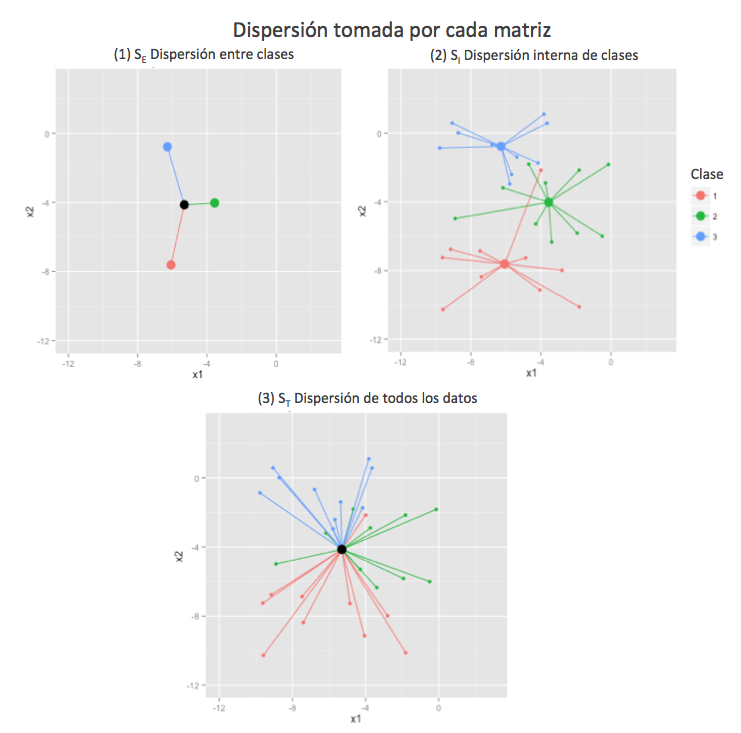
\includegraphics[width=1\textwidth]{Figures/Chapter2_SE_SI}	
  \caption[Distancias en las matrices de dispersión.]
  {En la gráfica (1) se representa la $S_E$, es decir las distancias al cuadrado entre la media de todos los datos (Punto negro) y las medias de cada clase (Puntos de color gruesos). La gráfica (2) representa $S_I$; es decir, la distancia al cuadrado de los individuos a la media de su clase. La gráfica (3) representa $S_T$, la dispersión de los datos con respecto a la media de todos.}
\end{figure}

Entre la matriz de dispersión interna $S_I$, la matriz de dispersión entre clases $S_E$ y la matriz de dispersión total $S_T$ existe una relación importante. Se cumple que $S_T = S_I + S_E $; es decir, la dispersión de las medias de grupos con la media global más la dispersión de cada clase individual es igual a la dispersión de los datos sin la información de las clases. Los datos de la figura 1.2 representan las distancias que toman en cuenta cada una de estas matrices. Para ejemplificar esta relación se generaron 10 datos por clase suponiendo distribuciones normales (El coeficiente de correlación de los datos generados es $-0.005$):

\begin{center}
\begin{tabular}{ c c c}
\toprule
\textbf{Clase} & \textbf{Distribución x1} & \textbf{Distribución x2} \\
\midrule\\
\addlinespace[-2ex]
1 & N(-5, 2.5) & N(-8, 2)\\
2 & N(-3, 2.5) & N(-4, 2)\\
3 & N(-7, 2.5) & N(-1, 2) \\
\addlinespace[1.5ex]
\bottomrule
\end{tabular}
\end{center}

Calculando las matrices de dispersión de acuerdo a las fórmulas (1.6), (1.7) y (1.8):

\begin{center}
\begin{tabular}{ c c c}
\toprule
\textbf{$S_I$} & \textbf{$S_E$} & \textbf{$S_T$} \\
\midrule\\
\addlinespace[-2ex]
$ \begin{bmatrix}  186.05 & 2.78 \\ 2.78 &  94.58 \end{bmatrix}$ &
$ \begin{bmatrix} 46.13 & -4.15 \\ -4.15 & 234.57 \end{bmatrix}$ &
$ \begin{bmatrix}  232.18 & -1.36 \\ -1.36 &  329.16 \end{bmatrix}$ \\
\addlinespace[1.5ex]
\bottomrule
\end{tabular}
\end{center}

De este ejemplo numérico se puede ver que al sumar la dispersión interna $S_I$ y la dispersión entre clases $S_E$ da como resultado la dispersión de todos los individuos $S_T$. En general este resultado se cumple, por lo que a continuación se enuncia esta relación que es muy fácil de demostrar.

\begin{proposition} \label{lemma2.1}
Sea $S_E$ la matriz de dispersión entre clases, $S_I$ la matriz de dispersión interna y $S_T$ la matriz de dispersión de los datos, entonces se tiene que cumplir la siguiente igualdad: $S_T$ = $S_I$ + $S_E$
\end{proposition}

Un problema muy común que surge en problemas de aprendizaje estadístico es que el costo computacional puede volverse intratable conforme la dimensionalidad de los individuos crece. En el ADLF se requiere hacer el cómputo de las matrices de dispersión de los individuos constantemente (o bien calcular la inversa de matrices de alta dimensionalidad), cálculos que para grandes dimensiones son sumamente costosos. Existen distintas maneras para hacer frente a este problema, uno de ellos involucra el PCA (Principal Component Analysis) en el preprocesamiento de los datos. Este método es fácil de calcular y solo requiere computar una vez la de matriz de dispersión \cite{ngo2012trace}. Debido a la finalidad de esta tesis no se profundizará en más técnicas para hacer frente a este problema, pero en textos como \cite{hastie2009elements}, \cite{duda2012pattern} aparecen distintos métodos para reducción de dimensionalidad.

Retomando el problema de cociente de trazas, lo que se busca es encontrar la proyección que mantenga juntos individuos de una clase al mismo tiempo que separa las medias de distintas clases. Una vez obtenida esta proyección se puede encontrar un hiperplano separador de los datos, o bien algún criterio para asignar la clase de pertenencia. 

\pagebreak
El problema de optimización se puede plantear como:
\begin{equation}\label{eq:2.5}
	\max_{\substack{V \in {\rm I\!R}^{n \times p} \\ V^TC V = I}} \frac{Tr(V^T S_E V)}{Tr(V^T S_I V)} 	
\end{equation}

 La solución a este problema no tiene una forma cerrada, por lo que en la literatura se buscan formulaciones alternas para resolverlo de una manera más sencilla \cite{wang2007trace} \cite{fukunaga2013introduction}, algunos ejemplos de estas formulaciones son:

\begin{equation}\label{eq:2.6}
	\max_{\substack{V \in {\rm I\!R}^{n \times p} \\ V^T S_I V = I}} Tr(V^T S_E V)
\end{equation}

\begin{equation} \label{eq:2.7}
	\max_{\substack{V \in {\rm I\!R}^{n \times p} \\ V^TC V = I}} Tr\left( \frac{V^T S_E V}{V^T S_I V}\right) 	
\end{equation}

\begin{equation} \label{eq:2.8}
	\max_{\substack{V \in {\rm I\!R}^{n \times p} \\ V^TC V = I}} \frac{|V^T S_E V|}{|V^T S_I V|} 	
\end{equation}

Con $|\bullet| = det(\bullet)$ y $Tr(\bullet) = Traza(\bullet)$.


En la siguiente parte de este capítulo se resolverá el problema original (1.9) para $p = 1$, para lo cual se introduce el cociente generalizado de Rayleigh. Para la generalización a $p$ dimensiones solo se plantea el problema y se proporcionan los casos en que la solución existe y es única. Seguido de esto se definirá una función $f(\rho)$ la cual sirve para encontrar el óptimo por métodos iterativos. Por último haciendo uso de los eigenvalores de $S_I$ y $S_E$ se darán cotas inferiores y superiores al óptimo.

\section{Problema del cociente de trazas}

El problema del cociente de trazas (Trace ratio problem) es fácil de ver cuando $V \in {\rm I\!R}^{n \times p}$ proyecta a un espacio de pocas dimensiones. Por ejemplo, cuando $p = 2$ se desea obtener la mejor proyección sobre un plano y cuando $p = 1$ sobre una recta. Para ejemplificar esta situación se creo un conjunto sintético donde cada $x_i \in {\rm I\!R}^{3}$. Las distribuciones son normales y se proyectan en ${\rm I\!R}^{2}$ y ${\rm I\!R}^{1}$. Los datos se pueden observar en la figura 1.3.

\begin{figure}[!ht]\label{Fig1.2}
  \centering
  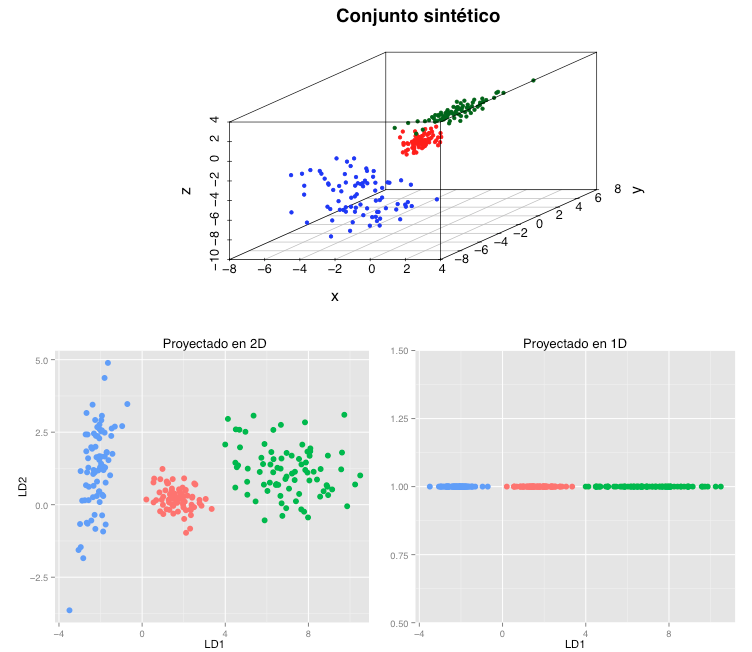
\includegraphics[width=1\textwidth]{Figures/Chapter2_1} 
  \caption[Mejores proyecciones en ${\rm I\!R}^{2}$ y ${\rm I\!R}$.]
  {En la gráfica de arriba se muestran los datos originales en 
   ${\rm I\!R}^{3}$ los cuales fueron generados a través de distribuciones normales con distintas medias y varianzas. En la gráfica de abajo a la izquierda se muestra la mejor proyección en ${\rm I\!R}^{2}$ y abajo a la derecha la mejor proyección en ${\rm I\!R}$}
\end{figure}

\subsection{Solución cuando p = 1}

El problema (1.9) toma la siguiente forma cuando $V \in {\rm I\!R}^{n}$. Se nombrara $v$ a este proyector de una dimensión ya que resulta ser solo un vector:


\begin{equation} \label{eq:2.9}
\max_{v \in {\rm I\!R}^{n}} \frac{v^T S_E v}{v^T S_I v}  
\end{equation}

Se tiene que $x_i \in {\rm I\!R}^{n}$ son los individuos originales con $i = 1 , ... , N $. Entonces sean $w_i \in {\rm I\!R}$ los individuos proyectados por el vector $v$ de manera que $w_i = v^Tx_i$. De esta manera es conveniente definir $\widehat{\mu}_k = v^T \mu_k$ y $\widehat{\mu} = v^T \mu$ como la media por clase y la media total de los datos proyectados.

\textbf{Matriz de dispersión entre clases $\Phi_{E}$ de los individuos proyectados $w_i$:}

$$\Phi_{E} = \sum\limits_{k =1}^{K} N_k (\widehat{\mu}_k - \widehat{\mu} )^2$$

$$\Phi_{E} = \sum\limits_{k =1}^{K} N_k (v^T \mu_k - v^T \mu)^2$$

$$\Phi_{E} =  \sum\limits_{k =1}^{K} N_k v^T ( \mu_k - \mu )(\mu_k - \mu )^T v $$
Por distributividad en matrices se cumple que $vAv+vBv =  v(A+B)v$, entonces:

\begin{equation}\label{eq:2.10}
\Phi_{E} = v^T \big[ \sum\limits_{k =1}^{K} N_k ( \mu_k - \mu )(\mu_k - \mu )^T \big] v	
\end{equation}

\textbf{Matriz de dispersión intra clase $\Phi_{I}$ de los individuos proyectados $w_i$}:
$$\Phi_{I} = \sum\limits_{k = 1}^{K} \sum\limits_{\substack{i = 1\\
                            y_i = k}}^{N} (w_i - \widehat{\mu}_k)^2 $$

$$\Phi_{I} = \sum\limits_{k = 1}^{K} \sum\limits_{\substack{i = 1\\
                            y_i = k}}^{N} (v_i^T x_i - v_i^T \mu_k)^{2} $$
$$\Phi_{I} =  \sum\limits_{k = 1}^{K} \sum\limits_{\substack{i = 1\\
                            y_i = k}}^{ N} v^T( x_i - \mu_k) ( x_i - \mu_k)^T v  $$

Usando de nuevo la distibutividad de matrices:

\begin{equation}\label{eq:2.11}
\Phi_{I} = v^T \big[ \sum\limits_{k = 1}^{K} \sum\limits_{\substack{i = 1\\
                            y_i = k}}^{ N} ( x_i - \mu_k) ( x_i - \mu_k)^T \big] v	
\end{equation}


 Las fórmulas de $\Phi_{I}$ y $\Phi_{E}$ de los individuos $w_i$ se pueden expresar en función de las matrices de dispersión intra clase y entre clases $S_I$ y $S_E$ de los individuos originales $x_i$. De esta manera:

 $$\Phi_{E} = f(S_E) = v^T S_E v$$
 $$\Phi_{I} = f(S_I) = v^T S_I v$$

Se tiene que $\Phi_{I}, \Phi_{E} \in {\rm I\!R}$, entonces maximizar el cociente $\frac{\Phi_{E}}{\Phi_{I}}$ con respecto a $v$ tiene como resultado una proyección que conserva cerca a los individuos pertenecientes a la misma clase, mientras que aleja a los centros de cada clase. Para el caso de una dimensión se puede encontrar una solución cerrada. La teoría asociada a este problema de maximización esta relacionada con el Cociente Generalizado de Rayleigh, el cual bajo las condiciones enunciadas de este caso, se puede transformar a un Cociente de Rayleight. Usando la proposición 1.2 se puede obtener la solución a este último.

\begin{proposition} \label{lemma2.2}
La solución a la maximización del Cociente de Rayleigh:
$$\max_{v \in {\rm I\!R}^{n} } \frac{v^T A v}{v^Tv} $$
cuando $A$ es simétrica, es obtenida cuando $v$ es el eigenvector asociado al eigenvalor más grande de la matriz $A$.
\end{proposition}


\subsection{Generalización a p dimensiones}

Para dimensiones más grandes de $v$, el Cociente Generalizado de Rayleigh no puede ser escrito en general como el Cociente de Rayleigh, por lo que la solución planteada en el capítulo anterior no es de utilidad. Esto genera la dificultad de no tener una solución cerrada, por lo que se han propuesto métodos iterativos y planteamientos alternos a la solución.

La generalización a $p$ dimensiones implica que los individuos $x_i \in {\rm I\!R}^{n}$ son proyectados ahora por la matriz $V = (V_1 | V_2 | ... |V_p)$, de manera que $w_i = V^T x_i$ con $w_i \in {\rm I\!R}^{p}$ y $V_j \in {\rm I\!R}^{n}$. De esta manera las matrices $\Phi_I$ y $\Phi_E$ se definen como sigue:

\begin{equation*}
\Phi_E = \sum\limits_{k = 1}^{K} N_{k} ||\widehat{\mu}_k - \widehat{\mu}||_2^2
\end{equation*}

\begin{equation*}
\Phi_E = \sum\limits_{k = 1}^{K} N_{k} ||V^T \mu_k - V^T \mu||_2^2
\end{equation*}

\begin{equation*}
\Phi_E = \sum\limits_{k = 1}^{K} N_{k} ||V^T (\mu_k - \mu)||_2^2
\end{equation*}


\begin{equation}\label{eq:2.17}
  \Phi_E = \sum\limits_{k = 1}^{K} N_{k} \big[ (V_1^T (\mu_k - \mu))^2 + (V_2^T (\mu_k - \mu))^2+ ... + (V_p^T (\mu_k - \mu))^2 \big]
\end{equation}

De esta expresión hay que destacar que $V_1^T (\mu_k - \mu)$ es un escalar, ya que $V_1 \in {\rm I\!R}^n$ y $(\mu_k - \mu) \in {\rm I\!R}^{n}$. Otra fórmula equivalente y que es comúnmente usada por sus propiedades algebraicas consiste en la siguiente expresión:

\begin{equation}\label{eq:2.18}
\Phi_E = \sum\limits_{k = 1}^{K} N_{k} Tr \big[ V^T (\mu_k - \mu) (\mu_k - \mu)^T V \big]	
\end{equation}

Para ejemplificarla se toma una clase $k = k_1$.  Al desarrollar $(\bullet) = V^T (\mu_1 - \mu) (\mu_1 - \mu)^T V$ se tiene una matriz en ${\rm I\!R}^{p \times p}$ igual a:


\begin{equation*}
(\bullet)= \left(\!
    \begin{array}{c}
      V_1^T (\mu_1-\mu)\\
      V_2^T (\mu_1-\mu)\\
      \vdots \\
      V_p^T (\mu_1-\mu)
    \end{array}
  \!\right) 
  \left(\!\begin{array}{c}
      (\mu_1-\mu)^T V_1 \quad
      (\mu_1-\mu)^T V_2 \quad
      \hdots \quad
      (\mu_1-\mu)^T V_p
    \end{array}
  \!\right) 
\end{equation*} 

\vspace{5mm}

\begin{equation*}
(\bullet)= \left(\!
    \begin{array}{ccc}
      V_1^T (\mu_1-\mu) (\mu_1-\mu)^T V_1 & \hdots & V_1^T (\mu_1-\mu) (\mu_1-\mu)^T V_p  \\
      V_2^T (\mu_1-\mu) (\mu_1-\mu)^T V_1 & \hdots & V_2^T (\mu_1-\mu) (\mu_1-\mu)^T V_p  \\
      \vdots & \ddots & \vdots\\
      V_p^T (\mu_1-\mu) (\mu_1-\mu)^T V_1 & \hdots & V_p^T (\mu_1-\mu) (\mu_1-\mu)^T V_p
    \end{array}
  \!\right) 
\end{equation*} 

\vspace{5mm}

\begin{equation*}
(\bullet)= \left(\!
    \begin{array}{ccc}
      (V_1^T (\mu_1-\mu))^2 & \hdots & V_1^T (\mu_1-\mu) (\mu_1-\mu)^T V_p \\
       V_2^T (\mu_1-\mu) (\mu_1-\mu)^T V_1  & \hdots & V_2^T (\mu_1-\mu) (\mu_1-\mu)^T V_p  \\
      \vdots & \ddots & \vdots\\
      V_p^T (\mu_1-\mu) (\mu_1-\mu)^T V_1  & \hdots & (V_p^T (\mu_1-\mu))^2
    \end{array}
  \!\right) 
\end{equation*} 

\vspace{5mm}

 Por lo tanto al calcular la traza de la matriz de $p \times p$ desarrollada arriba, se tiene que $Tr(V^T (\mu_1 - \mu) (\mu_1 - \mu)^T V)$ es equivalente a:
 \vspace{3mm}
 \begin{equation*}
Tr(\bullet) = (V_1^T (\mu_1-\mu))^2+ (V_2^T (\mu_1-\mu) )^2 + \hdots + (V_p^T (\mu_1-\mu) )^2
 \end{equation*}

Al generalizar a las $K$ clases y usando la propiedad de linealidad en la traza; es decir, $Tr(A+B) = Tr(A)+Tr(B)$, entonces se puede escribir de la siguiente manera:

\begin{equation*}
\Phi_E = Tr \sum\limits_{k = 1}^{K} N_{k}  \big[ V^T (\mu_k - \mu) (\mu_k - \mu)^T V \big]
\end{equation*}


Esta expresión es equivalente a (1.16). Como paso final se factoriza $V^T$ y $V$ sobre todos los sumandos, lo que nos llevaría a lo siguiente:

\begin{equation*} 
\Phi_E =  Tr (V^T \sum\limits_{k = 1}^{K} N_{k}  \big[(\mu_k - \mu) (\mu_k - \mu)^T \big] V)   
\end{equation*}

o, expresada en términos de $S_E = \sum\limits_{k = 1}^{K} N_{k}  \big[(\mu_k - \mu) (\mu_k - \mu)^T \big]$

\begin{equation}\label{eq:2.19}
\Phi_E =  Tr (V^T S_E V)     
\end{equation}

Similarmente se puede llegar a la formulación de la varianza intra-clase $\Phi_{I}$.
\begin{equation}\label{eq:2.20}
\Phi_{I} =  Tr (V^T S_I V )
\end{equation}



\subsection{Existencia de la solución}

Para demostrar la existencia y unicidad de la solución, las matrices $S_I$ y $S_E$ deben cumplir ciertas características. Sean $A = S_E$ y $B = S_I$, la primer condición que se les impone es que sean positivas definidas. La razón que apoya la restricción está relacionada con la forma de la función a maximizar, que es un cociente. Como $B$ se encuentra en el denominador, se tiene que evitar que $Tr(V^T B V) = 0$, ya que con este valor se indetermina la función objetivo \cite{ngo2012trace}. 

T.T. Ngo propone generalizar el estudio a las matrices positivas semidefinidas. Para esto se deben encontrar los casos en que $Tr(V^T B V)$ toma el valor de $0$. Si se diagonaliza a la matriz $B = Q \Lambda_{B} Q^T$ con $Q$ ortogonal y $\Lambda_{B}$ una matriz diagonal con entradas iguales a los eigenvalores de $B$, entonces:

\begin{equation*}
Tr(\Lambda_{B}) = \lambda_{B_1}+ \lambda_{B_2}+ ... +\lambda_{B_n} \qquad con \qquad \widehat{V} = Q^T V
\end{equation*}



De este modo $\widehat{V} = (\widehat{V}_1 | \widehat{V}_2 | ... | \widehat{V}_p)$ y cada $\widehat{V}_i^T = (\widehat{V}_{i1}, \widehat{V}_{i2}, ..., \widehat{V}_{in})$ es un vector renglón. De esta manera la matriz $\widehat{V}^T$:

\begin{equation*}
\widehat{V}^T = 	
\left(\!
    \begin{array}{c}
      \widehat{V}_1^T\\
      \widehat{V}_2^T\\
      \vdots \\
      \widehat{V}_p^T
    \end{array}
  \!\right)   = 
\left(\!
    \begin{array}{cccc}
      \widehat{V}_{11} & \widehat{V}_{12} & \hdots & \widehat{V}_{1n}\\
      \widehat{V}_{21} & \widehat{V}_{22} & \hdots & \widehat{V}_{2n}\\
      \vdots &  \vdots &\ddots & \vdots\\
      \widehat{V}_{p1} & \widehat{V}_{p2} & \hdots & \widehat{V}_{pn}\\
    \end{array}
  \!\right) 
\end{equation*}

Por lo que la traza que involucra a $B$ tiene la siguiente forma:

\begin{equation*}
Tr(V^T B V) = Tr(V^T Q \Lambda_{B} Q^T V) 	
\end{equation*}

\begin{equation*}
Tr(V^T B V)  = Tr(\widehat{V}^T \Lambda_{B} \widehat{V})
\end{equation*}

\begin{equation*}
V^T B V = 
\left(\!
    \begin{array}{c}
      \widehat{V}_1^T\\
      \widehat{V}_2^T\\
      \vdots \\
      \widehat{V}_p^T
    \end{array}
  \!\right) 
  \left(\!
    \begin{array}{cccc}
      \lambda_{B_1} & 0 & \hdots & 0\\
      0 & \lambda_{B_2} & \hdots & 0\\
      \vdots &  \vdots &\ddots & \vdots\\
      0 & 0 & \hdots & \lambda_{B_n}\\
    \end{array}
  \!\right) 
  \left(\!\begin{array}{c}
      \widehat{V}_1 |
      \widehat{V}_2 |
      \hdots |
      \widehat{V}_p
    \end{array}
  \!\right) 
\end{equation*} 

Desarrollando la multiplicación de matrices, y calculando la traza resulta en los siguientes sumandos:
 
 \begin{equation*}
\begin{aligned}
      Tr(V^T B V) =& \lambda_{B_1} \widehat{V}_{11}^2&  +
                     & \lambda_{B_2} \widehat{V}_{12}^2& +
                     & \hdots& +
                     &\lambda_{B_n} \widehat{V}_{1n}^2& + \\
                     & \lambda_{B_1} \widehat{V}_{21}^2&+
                     & \lambda_{B_2} \widehat{V}_{22}^2& +
                     & \hdots& +
                     &\lambda_{B_n} \widehat{V}_{2n}^2& + \\
                     & \vdots&  
                     & \vdots& 
                     & \vdots& 
                     & \vdots& \\
                     & \lambda_{B_1} \widehat{V}_{p1}^2&+
                     & \lambda_{B_2} \widehat{V}_{p2}^2& +
                     & \hdots& + 
                     & \lambda_{B_n} \widehat{V}_{pn}^2.&  
 \end{aligned}
 \end{equation*}

 Es fácil de ver que la expresión de arriba tiene $p \times n$ sumandos, por lo que se puede expresar en términos de dos sumatorias. La primera de $j=1,...,p$ y la segunda de $i = 1,...n$:

\begin{equation*} 
Tr(V^T B V) = \sum \limits_{j=1}^{p} \sum\limits_{i=1}^{n} \lambda_{B_i} \widehat{V}_{ji}^2
\end{equation*}

\begin{equation}\label{eq:2.21}
Tr(V^T B V) = \sum\limits_{i=1}^{n} \lambda_{B_i} \sum \limits_{j=1}^{p} \widehat{V}_{ji}^2    
\end{equation}

De la última expresión se separa la sumatoria sobre $i$. De esta manera, para cada elemento $i$ se tienen dos factores:

\begin{equation}\label{eq:2.22}
(i) \lambda_{B_i}
\end{equation}

 \begin{equation}\label{eq:2.23}
 (ii) \sum \limits_{j=1}^{p} \widehat{V}_{ji}^2   
 \end{equation}
 

 La idea para que $Tr(V^T B V)$ sea positivo, es que al menos uno de los sumandos sea positivo. Si (1.21) y (1.22) son ambos distintos de cero para al menos una $i$, entonces se cumple esta condición. Esta idea está expresada en el Lema 1.1.

\begin{lemma}\label{lemma2.4}
Sea $B$ positiva semidefinida y $V \in {\rm I\!R}^{n\times p}$. Si $B$ tiene a lo más $p-1$ eigenvalores iguales a $0$, entonces $Tr(V^T B V)  = Tr(\widehat{V}^T \Lambda_{B} \widehat{V}) \neq 0$  para cualquier matriz ortogonal $V$.
\end{lemma}

\begin{proof}
Sea $\widehat{V} = [\widehat{V}_1 | ... | \widehat{V}_p]$ tal que $\widehat{V} \widehat{V} = V^T Q Q^T V = V^T I_n V  = I_p$. De esta manera se puede construir una matriz $\widehat{V}' \in {\rm I\!R}^{p \times p}$ seleccionando $p$ de los $n$ renglones de $\widehat{V}$ tal que $\widehat{V}'$ sea no singular. $\widehat{V}'$ tiene la propiedad de no contener eigenvalores iguales a 0; como consecuencia, sus renglones y columnas no contienen al vector $\widehat{0}$. Al no contenerlo,se sabe que al menos hay $p$ renglones de $\widehat{V}$ tal que $\sum_{j=1}^{p}\widehat{V}_{ji}^2 \neq 0$ para cada uno de ellos. Por otra parte en el lema se supone que la matriz $B$ tiene a lo más $p-1$ eigenvalores iguales $0$ por lo que al menos un elemento de la sumatoria es distinto de cero.
\end{proof}

Analizando a mayor profundidad el resultado anterior, se sabe que hay $n-p+1$ eigenvalores de $B$ positivos ($\lambda_{B_i} \neq 0$) y $p$ renglones de $\widehat{V}$ que tienen norma distinta de cero. Al calcular la sumatoria (1.20), se tiene que al menos una combinación de $\lambda_{B_i}$ y uno de los $p$ renglones cumplen que su multiplicación tiene signo positivo. Para ejemplificar esta situación sean $C_i$ con $i = 1, ... , n-p+1$ los eigenvalores de $B$ y $K_j$ con $j = 1, ... , p$ la norma de los renglones de $\widehat{V}$ que son distintos de $0$.
 
\begin{center}
\begin{tabular}{ | c | c|  c | c|} 
\hline
$i$ & $\lambda_{B_i}$ & $\sum \limits_{j=1}^{p} \widehat{V}_{ji}^2$  & $\lambda_{B_i} \sum \limits_{j=1}^{p} \widehat{V}_{ji}^2$ \\ 
\hline
\hline
1 & $C_1$ & $0$ & $0$ \\ 
\hline
2 & $C_2$ & $0$ & $0$ \\ 
\hline
\vdots & \vdots & \vdots & \vdots \\ 
\hline
$n-p$ & $C_{n-p}$ & $0$ &  $0$\\ 
\hline
$n-p+1$ & $C_{n-p+1}$ & $K_{p}$ &  $C_{n-p+1} K_{p}$\\ 
\hline
$n-p+2$ & $0$ & $K_{p-1}$  & $0$ \\ 
\hline
\vdots & \vdots & \vdots & \vdots  \\ 
\hline
$n-1$ & $0$ & $K_2$ & $0$ \\ 
\hline
$n$ & $0$ & $K_1$ & $0$ \\ 
\hline
\hline

\end{tabular}
\end{center}

Con esta combinación se tiene que al menos hay un sumando de $\sum\limits_{i=1}^{n} \lambda_{B_i} \sum \limits_{j=1}^{p} \widehat{V}_{ji}^2 $ distinto de cero, por lo que $Tr(V^T B V) \neq 0$. Bajo estas condiciones se garantiza que el denominador sea mayor a 0, solo falta asegurarse que el numerador sea menor a infinito.

\begin{lemma}
Sea $U_p = \{ V \in {\rm I\!R}^{n \times p} | V^T V = I_p \} $ un conjunto compacto con $V = (v_1, v_2, ... , v_p)$
\end{lemma}
\begin{proof}
Se tiene que $U_p$ es un conjunto cerrado porque contiene a todos sus puntos límite; por otro lado, $U_p$ también es acotado bajo la norma 2 y la norma de Frobenius:

Tomando la norma-2 y la norma de Frobenius de $V$: 
\begin{equation*}
\begin{aligned}
	||V||_2 =& Max \{||V_x ||_2 \quad | \quad ||x||_2 = 1 \} \\
		    =& ||V_x||^2_2  \\
		    =& (Vx)^T (Vx) \\
		    =& x^T V^T V x\\
		    =& x^T x = 1\\
	||V||_F	=& \sum\limits_{F}^{p} ||v_i|| = p   
\end{aligned}
\end{equation*}

Entonces se tiene $U_p$ es cerrado y acotado, por lo que $U_p$ es compacto.
\end{proof}

Con este resultado se tiene que $Tr(V^T A V)$ toma un valor finito ya que todas sus entradas son finitas. 


\begin{lemma}\label{lemma2.5}
Sean $A$ y $B$ dos matrices simétricas tales que $B$ es positiva semidefinida con rango mayor que $n-p$; es decir, que tenga al menos $n-p+1$ eigenvalores distintos de cero. Entonces el cociente $(1.9)$ admite un máximo con valor $\rho^*$ \cite{ngo2012trace}.
\end{lemma}

\begin{proof}
Tomando el resultado del lema 1.1 se tiene que $Tr(V^T B V) \neq 0$; por otra parte, $V \in U_p$ que es un conjunto compacto. Con estas dos observaciones, el valor de (1.9) es distinto de infinito. Entonces el cociente $(1.9)$ admite un máximo con valor $\rho^*$ y que tiene como argumento $V^{**}$.
\end{proof}

\subsection{Equivalencia con un problema escalar}

\textbf{Valor en el óptimo}. Del lema 1.3 se sabe que existe una matriz $V^{**} \in U_p$ tal que (1.9) alcanza el valor máximo $\rho^*$. Expresando esta idea se tiene que:

\begin{equation} \label{eq:2.24}
 \frac{Tr(V^{T**} A V^{**})}{Tr(V^{T**} B V^{**})} = \rho^* 
\end{equation}

Entonces para cualquier otra matriz $V \in U_p $:

\begin{equation}\label{eq:2.25}
 \frac{Tr(V^T A V)}{Tr(V^T B V)} \leq \rho^* 
\end{equation}

Como la traza es un operador lineal y por la propiedad distributiva de las matrices entonces (1.24) es equivalente a:

\begin{equation*}
 Tr(V^T A V)- \rho^* Tr(V^T B V) \leq 0 
\end{equation*}

\begin{equation*}
	Tr(V^T A V- \rho^* V^T B V) \leq 0	
 \end{equation*}

 \begin{equation} \label{eq:2.26}
	Tr(V^T (A - \rho^* B )V) \leq 0	
 \end{equation}

y el resultado equivalente para (1.23):
	
 \begin{equation} \label{eq:2.27}
	Tr(V^{T**} (A - \rho^* B )V^{**}) = 0	
 \end{equation}


Para facilitar la lectura, de aquí en adelante se define la función $G(\rho) = A- \rho B$. Maximizar el lado izquierdo de la desigualdad (1.25) sujeto a $V^T V = I$ es equivalente a maximizar un problema de eigenvalores generalizado. Usando lo establecido en el apéndice A, se sabe que el valor máximo de este problema dado $\rho^*$:

\begin{equation}\label{eq:2.28}
	\max_{\substack{V \in {\rm I\!R}^{n \times p} \\ V^T V = I}} Tr(V^T G(\rho^*) V) = \lambda_{G(\rho^*)_1} + \lambda_{G(\rho^*)_2} + ... + \lambda_{G(\rho^*)_p}
\end{equation}
  
 Con $\lambda_{G(\rho^*)_1} \geq \lambda_{G(\rho^*)_2} \geq ... \geq \lambda_{G(\rho^*)_p}$ los $p$ eigenvalores más grandes de $G(\rho^*)$. De esta manera el valor óptimo de (1.27) es simplemente la suma de los $p$ eigenvalores más grandes de esta matriz, y $V^{**}$ el conjunto de correspondientes eigenvectores. Para obtener este valor y la matriz, el primer paso es encontrar a $\rho^*$, ya que teniéndolo es inmediato calcular $V^{**}$. Dada esta premisa, se puede ver que el problema a resolver se reduce a buscar el valor óptimo de $\rho$. Para esto se define la función $f(\rho)$ sobre todo $\rm I\!R$, tal que $f(\rho)$ es continua sobre su argumento $\rho$: 

\begin{equation}  \label{eq:2.29}
	f(\rho) = \max_{V^T V = I} Tr(V^T (G(\rho)) V)
\end{equation}

Es conveniente examinar $f(\rho)$ con dos objetivos, el primero es estimar la dificultad de calcular el valor de $f(\rho)$ y el segundo es encontrar la maximización adecuada para obtener $\rho^*$. Respecto al primer punto, la manera de calcular $f(\rho)$ en cada punto es equivalente a (1.27), pero en lugar de usar los eigenvalores de $G(\rho^*)$ se usan los de $G(\rho)$. En particular se llamará $V(\rho)^*$ al argumento que resuelve (1.28) \footnote{Se utilizó la nomenclatura de $V(\rho^*)$ porque estos eigenvectores dependen del valor de $\rho$ en la matriz $A - \rho B$.}. Sean $\lambda_{G(\rho)_1} \geq \lambda_{G(\rho)_2} \geq ... \geq \lambda_{G(\rho)_n}$ los $n$ eigenvalores de $G(\rho)$. Con esta notación $f(\rho)$ toma el valor de:


\begin{equation}\label{eq:2.30}
f(\rho) = \lambda_{G(\rho)_1} + \lambda_{G(\rho)_2} + ... +\lambda_{G(\rho)_p}
\end{equation}


Para el segundo punto, la idea es iterar hasta obtener el valor de $\rho^*$. Por esto, es conveniente analizar como se comporta la función con respecto a su argumento. A continuación se presentan dos propiedades de $f(\rho)$. Para demostrarlas, primero se enuncia el teorema 8.1.5 de \cite{golub2012matrix}.

\begin{theorem} \label{teorem.1}
	
	Sean $X$ y $X+E$ matrices simétricas $n \times n$, y $\lambda_{X_k}$, $\lambda_{E_k}$ los k-ésimos eigenvalores más grandes de $X$ y $E$ respectivamente. De esta manera $\lambda_{X_k}$ es el k-ésimo eigenvalor más grande de $X$ y $\lambda_{E_1}$ el más grande de $E$. Con estas definiciones se cumple lo siguiente:

	\begin{equation}\label{eq:2.31}
		\lambda_{X_k} +\lambda_{E_n} \leq \lambda_{(X+E)_k} \leq \lambda_{X_k} +\lambda_{E_1}
	\end{equation}

\end{theorem}

Se procede a enunciar este lema acerca de la función $f(\rho)$

\begin{lemma}\label{lemma2.6}
La función $f(\rho) = \max_{V^T V = I} Tr(V^T (A - \rho B) V)$ cumple las siguientes dos propiedades: 

(1) $f$ es una función no creciente de $\rho$ \\
(2) $f(\rho)= 0$  si y solo si $\rho = \rho^*$
\end{lemma}

Para probar la parte $(1)$ del lema 1.4 se comparan los valores de $f(\rho)$ para $\rho_1$ y $\rho_2$ con $\rho_2 \geq \rho_1$. Como se desea demostrar que $f$ es una función no creciente de $\rho$, se busca que $f(\rho_2) \leq f(\rho_1)$. Se definen las matrices $Y=X+E$ y $E = Y-X$, para después restarles $\lambda_{X_k}$, entonces (1.29) se puede escribir como:

\begin{equation*}
		\lambda_{(X)_k} +\lambda_{(Y-X)_n} \leq \lambda_{(Y)_k} \leq \lambda_{(X)_k} +\lambda_{(Y-X)_1}
\end{equation*}

\begin{equation*}
		\lambda_{(Y-X)_n} \leq \lambda_{(Y)_k} - \lambda_{(X)_k} \leq \lambda_{(Y-X)_1}
\end{equation*}

La expresión en el centro de estas desigualdades es la resta del eigenvalor k-ésimo de la matriz $X$ y $Y$, por lo que si se realiza la suma de $k = 1$ a $k = p$ se tiene lo siguiente:

\begin{equation}\label{eq:2.32}
		p \lambda_{(Y-X)_n} \leq \sum_{k=1}^{p} \lambda_{(Y)_k} - \sum_{k=1}^{p} \lambda_{(X)_k} \leq  p \lambda_{(Y-X)_1}
\end{equation}

Definiendo $X = A - \rho_2 B$ y $Y = A - \rho_1 B$, entonces (1.31) toma la siguiente forma:

\begin{equation}\label{eq:2.33}
    p \lambda_{(B(\rho_2-\rho_1))_n} \leq \sum_{k=1}^{p} \lambda_{(A - \rho_1 B)_k} - \sum_{k=1}^{p} \lambda_{(A - \rho_2 B)_k} \leq  p \lambda_{(B(\rho_2-\rho_1))_1}
\end{equation}

Retomando el resultado (1.29), y sustituyéndolo en (1.32) la desigualdad queda de la siguiente forma:

\begin{equation}\label{eq:2.34}
		p \lambda_{(B (\rho_2 - \rho_1))_n} \leq f(\rho_1) - f(\rho_2) \leq  p \lambda_{(B (\rho_2 - \rho_1))_1}
\end{equation}


En la parte izquierda de la desigualdad anterior, se puede a determinar el signo que toman los eigenvalores $\lambda_{(B (\rho_2 - \rho_1))_n}$. 
Si $(\rho_2- \rho_1) \geq 0$ entonces la matriz $(\rho_2 - \rho_1)B$ es positiva semidefinida; por lo tanto, todos sus eigenvalores son mayores o iguales a 0:

\begin{equation*}
	0 \leq p \lambda_{(B (\rho_2 - \rho_1))_n} \leq f(\rho_1) - f(\rho_2) \leq  p \lambda_{(B (\rho_2 - \rho_1))_1}
\end{equation*}
	
\begin{equation}\label{eq:2.35}
	0 \leq f(\rho_1) - f(\rho_2)
\end{equation}

De esta manera $f(\rho_2)  \leq  f(\rho_1) $ cuando $\rho_2 \geq \rho_1$

Para probar la parte (2) del lema 1.4, se tiene que demostrar la condición suficiente y la condición necesaria. La demostración de la primera es inmediata, ya que cuando $\rho = \rho^*$, entonces por (1.26), $f(\rho) = 0$. Para la condición necesaria se usará (1.23) y la propiedad que la $Tr(V^T B V) >0 \enspace \forall \enspace V \in U_p$. Se demostrará que, dado $f(\rho^*) = 0$, entonces:


\begin{equation}\label{eq:2.36}
	(i) \quad f(\rho) < 0 \quad si \quad \rho>\rho^*
\end{equation}
\begin{equation}\label{eq:2.37}
	(ii) \quad f(\rho) > 0 \quad si \quad \rho<\rho^*
\end{equation}

\underline{\textbf{Caso (i) $\rho > \rho^* $}}

Se tiene que las siguientes desigualdades se cumplen:
\begin{equation*}
\frac{Tr(V^T A V)}{Tr(V^T B V)} \leq \rho^* < \rho	
\end{equation*}

Por lo que es equivalente a:

\begin{equation*}
	Tr(V^T (A -\rho B)V) < 0 \quad \forall V \in U_p
\end{equation*}


De esta manera $f(\rho) < 0$ cuando $\rho > \rho^*$.
\vspace{5mm}

\underline{\textbf{(ii) $\rho < \rho^* $}}

Retomando el resultado (1.24) y suponiendo que $\rho^* > \rho$ entonces existe una $V^{*}$ tal que:


 \begin{equation*} 
 \rho < \frac{Tr(V^{T*} A V^*)}{Tr(V^{T*} B V^*)} \leq \rho^*
 \end{equation*}

\begin{equation*}
Tr(V^{T*} A V^* - \rho V^{T*} B V^*) > 0 \quad \Longrightarrow \quad \frac{Tr(V^{T*} A V^*)}{Tr(V^{T*} B V^{*})} > \rho
\end{equation*}

En particular:

\begin{equation*}
\max_{V^TV} \frac{Tr(V^{T} A V)}{Tr(V^{T} B V)} > \rho
\end{equation*}

De esta manera $f(\rho) > 0$ cuando $\rho < \rho^*$.


Las ecuaciones (1.35) (1.36), junto con la continuidad de la funcion $f$, muestran que $f(\rho) = 0$ implica $\rho = \rho^*$ \cite{ngo2012trace}. De esta manera el problema puede ser visto como encontrar la raíz de la función $f(\rho)$. La figura 1.4 muestra como es esta función.

\begin{corollary}
La función $f(\rho) = \max_{V^TV = I} Tr(V^T (A -\rho B)V)$ cumple las siguientes condiciones:

$$f(\rho) > 0  \quad \forall \quad \rho \in (-\inf, \rho^*)$$
$$f(\rho) < 0  \quad \forall \quad \rho \in (\rho^*, \inf)$$

\end{corollary}

\begin{figure}[!ht]\label{Fig1.3}
  \centering
	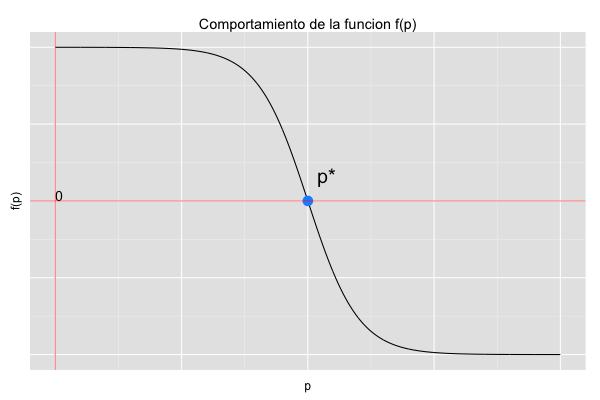
\includegraphics[width=1\textwidth]{Figures/Chapter2_fp}	
  \caption[Comportamiento de $f(\rho)$.]
  {La función $f(\rho)$ es no creciente para toda $\rho$. El valor de $f(\rho) = \lambda_{G(\rho)1}+ \lambda_{G(\rho)2} + ... +\lambda_{G(\rho)p}.$ $f(\rho^*) = 0 $}
\end{figure}


\begin{example} \label{ex:1}
Para ejemplificar el lema 1.4 se muestran las matrices $A,B \in {\rm I\!R}^{3 \times 3}$. Para el valor de $f(\rho)$ se utiliza la propiedad (1.29):

$$f(\rho) = \lambda_{G(\rho)1} + \lambda_{G(\rho)2} + ... + \lambda_{G(\rho)p}$$

con $p$ la dimensión a la que se va a proyectar. 


\begin{equation*}
A = \left(\!
    \begin{array}{ccc}
      4 & 0 & 0 \\
      0 & 6 & 0 \\
      0 & 0 & 8 
    \end{array}
  \!\right), \quad
B = \left(\!
    \begin{array}{ccc}
      1.5 & 0 & 0 \\
      0 & 2.5 & 0 \\
      0 & 0 & 5 
    \end{array}
\!\right) 
\end{equation*}



\begin{equation*}
G(\rho) = A- \rho B = \left(\!
    \begin{array}{ccc}
      4-1.5\rho & 0 & 0 \\
      0 & 6-2.5\rho & 0 \\
      0 & 0 & 8-5\rho 
    \end{array}   	
      \!\right) 
\end{equation*}

Los eigenvalores de esta matriz son $4-1.5\rho$,  $6-2.5\rho$ y  $8-5\rho$. Las funciones graficadas de estos eigenvalores se presentan en la figura 1.5.

\begin{figure}[!ht] \label{Fig1.4}
  \centering
  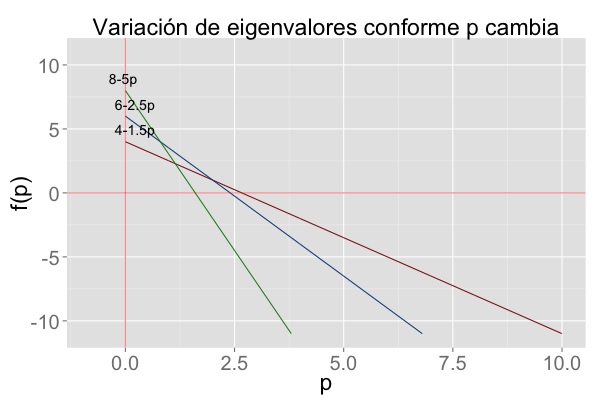
\includegraphics[width=1\textwidth]{Figures/Chapter2_3eigen}  
  \caption[Gráfica de los eigenvalores en función de $\rho$.] {Cada línea representa como se comporta cada eigenvalor de $A- \rho B$ cuando se varía $\rho$.}
\end{figure}

Cuando se desea que el proyector sea de dimensión 1, entonces se tiene que $f(\rho)$ es el eigenvalor más grande,  cuando sea de dimensión 2, la suma de los dos más grandes y así respectivamente. El valor de $f(\rho)$ para estos tres casos está representado en la figura 1.5.

\begin{figure}[!ht] \label{Fig1.5}
  \centering
  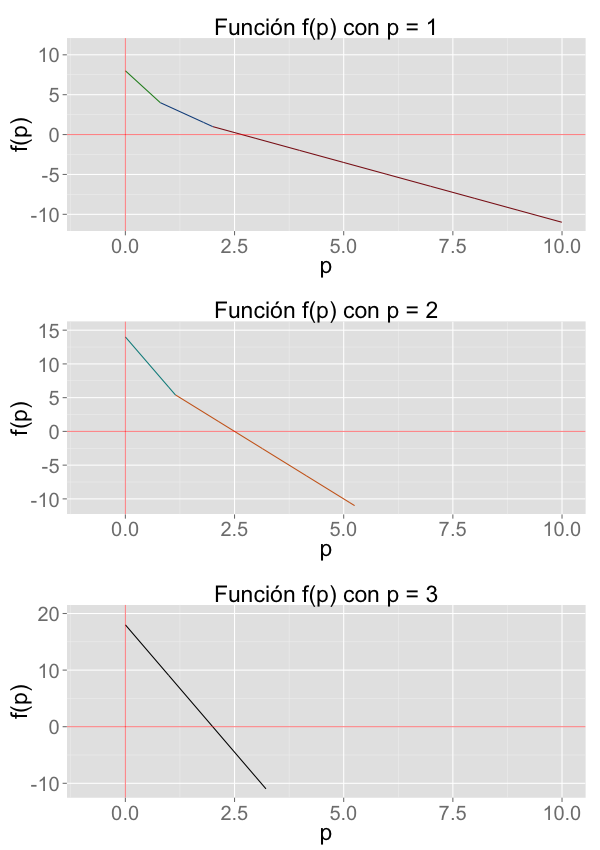
\includegraphics[width=1\textwidth]{Figures/Chapter2_grid3eigen}  
  \caption[$f(\rho)$ para proyectores de 1,2 y 3 dimensiones.] {La figura superior representa a $f(\rho) = \lambda_{G(\rho)_1}$, la de enmedio $f(\rho) = \lambda_{G(\rho)_1} + \lambda_{G(\rho)_2}$ y la de abajo $f(\rho) = \lambda_{G(\rho)_1} + \lambda_{G(\rho)_2} + \lambda_{G(\rho)_3}$.}
\end{figure}

\end{example}
\pagebreak

\subsection{Localización del óptimo}

En la sección anterior se encontró que la maximización al cociente de trazas puede ser visto como el problema de encontrar la raíz de la función $f(\rho) = max_{V^T V= I} Tr(V^T(A-\rho B)V)$. Por esto, encontrar un intervalo $(\rho_1, \rho_2)$ que contenga al valor óptimo $\rho^*$ puede reducir el número de iteraciones del método. Usando el lema 1.4 se sabe que $f$ es una función no creciente de $\rho$. Por esta razón si se encuentra una $\rho_1$ y $\rho_2$ tal que $f(\rho_1) \geq 0$ y $f(\rho_2) \leq 0$ y con la propiedad de continuidad de la funcion $f(\rho)$ entonces se encontró un intervalo que contiene a $\rho^*$. 

En esta tesis se dan cotas para el valor de $\rho^*$, la primera en función los eigenvalores de una transformación de $B -\rho A$ y la segunda en función de los eigenvalores de $B$ y $A$ \cite{ngo2012trace}. La demostración de cada una requiere del conocimiento del concepto de inercia y del Teorema de la Inercia de Sylvester. Por este motivo se presentan a continuación: \footnote{La demostración de este teorema puede ser encontrada en \cite{golub2012matrix}.}

\begin{definition}
La inercia de una matriz simétrica $A$ es la tripleta de enteros no negativos $(m, z, p)$ donde $m$, $z$ y $p$ son respectivamente el número de eigenvalores negativos, cero y positivos de $A$ \cite{golub2012matrix}.
\end{definition}

\begin{theorem}\label{teorem.2}
Sea $A \in {\rm I\!R}^{n \times n}$ una matriz simétrica y $Z \in {\rm I\!R}^{n \times n}$ no singular. Entonces $A$ y $Z^T A Z$ tienen la misma inercia \cite{golub2012matrix}.
\end{theorem}

\begin{proposition}
La raíz $\rho^*$ de $f(\rho)$ está localizada en el intervalo $(\lambda_p, \lambda_1)$ donde $\lambda_p$ es el p-ésimo eigenvalor más grande de $Z^T(A-\rho B)Z$.
\end{proposition}

\begin{proof}
Sea $Z$ la matriz que diagonaliza a $A-\rho B$ de manera que\footnote{El cálculo de esta matriz puede obtenerse en el algoritmo 8.7.1 de \cite{golub2012matrix}}:

\begin{equation}\label{eq:2.38}
\begin{aligned}
 Z^T AZ = \Lambda \\ Z^T B Z = I
 \end{aligned}
\end{equation}

Con $\Lambda$ una matriz diagonal y $\mu_1, \ldots,  \mu_n$ sus respectivos eigenvalores e $I$ la identidad de tamaño $n$. Entonces por el teorema 1.2 se sabe que $A- \rho B$ y $Z^T(A- \rho B)Z = \Lambda -\rho I$ tienen el mismo número de eigenvalores positivos, negativos y cero. Por lo tanto, la matriz en cuestión es de la siguiente forma:

\begin{equation}\label{eq:2.39}
\Lambda - \rho I = 
\left(\!
    \begin{array}{cccc}
      \mu_1 & 0 & \hdots & 0\\
      0 & \mu_2 & \hdots & 0\\
      \vdots & \vdots & \ddots & \vdots \\
      0 & 0 & \hdots & \mu_n
    \end{array}
  \!\right) - \rho
  \left(\!
    \begin{array}{cccc}
      1 & 0 & \hdots & 0\\
      0 & 1 & \hdots & 0\\
      \vdots & \vdots & \ddots & \vdots \\
      0 & 0 & \hdots & 1
    \end{array}
  \!\right) 
\end{equation} 

Como la  matriz $V$ de (1.9) es de tamaño $n \times p$, solo nos interesa saber el signo de los $p$ eigenvalores más grandes. Tomando $\rho = \mu_p$ entonces los elementos de la diagonal de la matriz $\Lambda- \rho I$ son de la forma:


\begin{equation}\label{eq:2.40}
\begin{aligned}
   \mu_i - \mu_p & \geq 0  \quad para \quad i \geq p\\
   \mu_i - \mu_p & \leq 0  \quad para \quad i \leq p
\end{aligned}
\end{equation} 

Los primeros p elementos tienen la propiedad de ser no negativos, ya que $\lambda_{(A-\rho B)_1} \geq \lambda_{(A-\rho B)_2} \geq ... \geq \lambda_{(A-\rho B)_p}$. Usando el teorema 1.2 se sabe que los primeros p eigenvalores de $A-\rho B$ también son no negativos. Por ende la suma de ellos es mayor o igual que cero. 

Por otro lado si se toma $\rho = \mu_1$. Entonces los elementos de la diagonal de la matriz (1.38) son de la forma:

\begin{equation}\label{eq:2.41}
   \mu_i - \mu_1  \leq 0 \quad \forall \quad i
\end{equation} 

Con $i = 1, ..., p$, cada uno de los elementos de la diagonal tiene la propiedad de ser no positivo por el mismo argumento que el caso pasado. Por lo tanto los $p$ eigenvalores más grandes de $\Lambda - \rho I$ y de $A-\rho B$ son no positivos, por lo que su suma es menor o igual que cero:

\begin{equation}\label{eq:2.42}
  \rho = \mu_p  \Rightarrow \sum_{i=1}^{p} (\mu_i- \mu_p) \geq 0 \Rightarrow f(\rho) \geq 0
\end{equation}

\begin{equation}\label{eq:2.43}
  \rho = \mu_1  \Rightarrow \sum_{i=1}^{p} (\mu_i - \mu_1) \leq 0 \Rightarrow f(\rho) \leq 0
\end{equation}

\end{proof}

\pagebreak

\begin{example} \label{ex:2}
Tomando las matrices A,B iguales que en el ejercicio 1.1, se puede encontrar fácilmente a la matriz $Z$:


\begin{equation*}
Z = \left(\!
    \begin{array}{ccc}
      \sqrt(\frac{1}{1.5}) & 0 & 0 \\
      0 & \sqrt(\frac{1}{2.5}) & 0 \\
      0 & 0 & \sqrt(\frac{1}{5}) 
    \end{array}
  \!\right)
\end{equation*}

Con la matriz $Z$ definida de esta manera, $Z^T A  Z = \Lambda$ y $Z^T B Z = I$ toman la siguiente forma:

\begin{equation*}
\Lambda - \rho I = 
\left(\!
    \begin{array}{ccc}
      \frac{4}{1.5} & 0  & 0\\
      0 & \frac{6}{2.5}  & 0\\
      0 & 0 & \frac{8}{5}
    \end{array}
  \!\right) - \rho
  \left(\!
    \begin{array}{ccc}
      1 & 0 & 0\\
      0 & 1 & 0\\
      0 & 0 & 1
    \end{array}
  \!\right) 
\end{equation*}

Entonces se puede encontrar un intervalo tal que $\rho^* \in \big[\rho_1, \rho_2 \big]$:

\begin{equation*}
  \begin{aligned}
\rho_1 &= \mu_p \\
\rho_2 &= \mu_1  
  \end{aligned}
\end{equation*}

Conforme el tamaño de la dimensión a proyectar cambia, las cotas son las siguientes:

\begin{equation*}
  \begin{aligned}
  p =& 1 \Rightarrow \qquad \rho_1 = \frac{4}{1.5} \quad y \quad \rho_2 = \frac{4}{1.5}\\
  p =& 2 \Rightarrow \qquad \rho_1 = \frac{4}{1.5} \quad y \quad \rho_2 = \frac{6}{2.5} \\
  p =& 3 \Rightarrow \qquad \rho_1 = \frac{4}{1.5} \quad y \quad \rho_2 = \frac{8}{5}
  \end{aligned}
\end{equation*}
 

 Estas cotas se pueden ver más fácil en la figura 1.6,donde se observa $f(\rho)$ con respecto a $p$:

\begin{figure}[!ht] \label{Fig1.6}
  \centering
  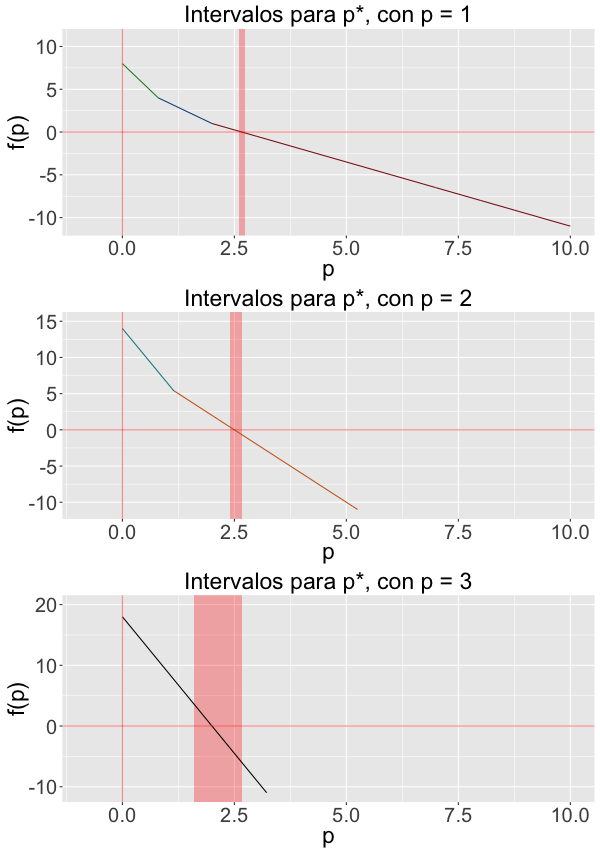
\includegraphics[width=.9\textwidth]{Figures/Chapter2_grid3eigen_interv}  
  \caption[Intervalos para $\rho^*$.] {La figura superior representa intervalos para $\rho^*$ cuando $f(\rho) = \lambda_{G(\rho)_1}$, la de enmedio cuando $f(\rho) = \lambda_{G(\rho)_1} + \lambda_{G(\rho)_2}$ y la de abajo cuando $f(\rho) = \lambda_{G(\rho)_1} + \lambda_{G(\rho)_2} + \lambda_{G(\rho)_3}$.}
\end{figure}

\end{example}

Otro intervalo que se ha desarrollado tiene que ver con directamente con los eigenvalores de $A$ y $B$ en lugar de los obtenidos por la matriz $A-\rho B$:

\pagebreak
\begin{proposition}
Sea $B$ positiva definida, entonces la raíz $\rho^*$ de $f(\rho)$ es tal que \cite{ngo2012trace}:

\begin{equation*}
\frac{\sum_{i = 1}^{p}\lambda_{A_i}}{\sum_{i = 1}^{p}\lambda_{B_i}} \leq \rho^* \leq \frac{\sum_{i = 1}^{p}\lambda_{(A)_i}}{\sum_{i = 1}^{p}\lambda_{(B)_{n-i+1}}}	
\end{equation*}

con $\lambda_{A_i}$ y $\lambda_{B_i}$ el i-ésimo eigenvalor más grande  de la matriz $A$ y $B$ respectivamente \cite{ngo2012trace}. 
\end{proposition}


\begin{proof}
Se tiene la propiedad que para una $p$ dada:


\begin{equation}\label{eq:2.44}
\max_{V^T V = I} Tr(V^T A V) =  Tr(V^{T*} A V^*) = \sum_{i=1}^p \lambda_{A_i }
\end{equation}
 
Con $\lambda_{A_i}$ los eigenvalores de A. Como esta $V^*$ maximiza la traza sobre $A$, entonces no necesariamente maximiza la de $B$. Al sustituirla en $Tr(V^{T} B V)$ se tiene que: 

\begin{equation}\label{eq:2.45}
Tr(V^{T*} B V^*) \leq \sum_{i=1}^p \lambda_{B_i }
\end{equation}

Con $\lambda_{B_i}$ los eigenvalores de B. Al hacer el cociente de (1.43) y (1.44) Se puede acotar inferiormente a $\rho^*$:


\begin{equation*}
  \frac{\sum_{i=1}^p \lambda_{A_i}} {\sum_{i=1}^p \lambda_{B_i}} \leq \frac{Tr(V^{T*} A V^*)}{Tr(V^{T*} B V^*)} \leq \max_{V^T V} \frac{Tr(V^{T} A V)}{Tr(V^{T} B V)} = \rho^*
\end{equation*}

Ahora falta acotarlo superiormente. Usando las siguientes propiedades que son derivadas de (1.27):

\begin{equation}\label{eq:2.46}
  Tr(V^T A V) \leq \sum_{i=1}^p \lambda_{A_i} 
\end{equation}

\begin{equation}\label{eq:2.47}
  Tr(V^T B V) \geq \sum_{i=1}^p \lambda_{B_{(n-i+1)}}
\end{equation}

La expresión (1.46) es la suma de los p eigenvalores más chicos de $B$. Dividiendo (1.45) entre (1.46) se tiene que para cualquier matriz ortogonal $V$:

\begin{equation}\label{eq:2.48}
   \frac{Tr(V^{T} A V)}{Tr(V^{T} B V)} \leq \frac{\sum_{i=1}^p \lambda_{A_i}}{\sum_{i=1}^p \lambda_{B_{(n-i+1)}}}
\end{equation}

En particular si se toma $V = V^{**}$ (La matriz con la que se alcanza $\rho^*)$:

\begin{equation}\label{eq:2.49}
  \rho^* = \frac{Tr(V^{T**} A V^{**})}{Tr(V^{T**} B V^{**})} \leq \frac{\sum_{i=1}^p \lambda_{A_i}}{\sum_{i=1}^p \lambda_{B_{(n-i+1)}}}
\end{equation}

\end{proof}
\begin{example}
Para ejemplificar esta cota se usará las matrices $A$ y $B$ de los dos ejemplos anteriores y se muestra en la figura 1.7.


\begin{equation*}
A = \left(\!
    \begin{array}{ccc}
      4 & 0 & 0 \\
      0 & 6 & 0 \\
      0 & 0 & 8 
    \end{array}
  \!\right), \quad
B = \left(\!
    \begin{array}{ccc}
      1.5 & 0 & 0 \\
      0 & 2.5 & 0 \\
      0 & 0 & 5 
    \end{array}
\!\right) 
\end{equation*}


(i) Para $p = 1$ la cota es la siguiente:
\begin{equation*}
\begin{aligned}
  \lambda_{A_1} = 8 \qquad
  \lambda_{B_1} = 5 \qquad
  \lambda_{B_3} = 1.5
\end{aligned}
\end{equation*}

\begin{equation*}
\begin{aligned}
\rho_1 = \frac{\sum_{i = 1}^{p}\lambda_{A_i}}{\sum_{i = 1}^{p}\lambda_{B_i}}  = \frac{8}{5} \qquad
\rho_2 = \frac{\sum_{i = 1}^{p}\lambda_{A_i}}{\sum_{i = 1}^{p}\lambda_{B_{n-i+1}}}  = \frac{8}{1.5}
\end{aligned}
\end{equation*}

(ii) Para $p = 2$ la cota es la siguiente:

\begin{equation*}
\begin{aligned}
\sum_{i = 1}^{2}\lambda_{A_1}  =& 14 \qquad
\sum_{i = 1}^{2}\lambda_{B_1}  =& 7.5 \qquad
\sum_{i = 1}^{2}\lambda_{B_{3-i+1}} =& 4
\end{aligned}
\end{equation*}

\begin{equation*}
\begin{aligned}
\rho_1 = \frac{\sum_{i = 1}^{p}\lambda_{A_i}}{\sum_{i = 1}^{p}\lambda_({B_i)}}
 = \frac{14}{7.5} \qquad
\rho_2 = \frac{\sum_{i = 1}^{p}\lambda_{A_i}}{\sum_{i = 1}^{p}\lambda_{B_{n-i+1}}}  = \frac{14}{4}
\end{aligned}
\end{equation*}



(iii) Para $p = 3$ la cota es la siguiente:
\begin{equation*}
  \begin{aligned}
  \sum_{i = 1}^{3}\lambda_{A_1}  = 18 \qquad
  \sum_{i = 1}^{3}\lambda_{B_1}  = 9 \qquad
  \sum_{i = 1}^{3}\lambda_{B_{n-i+1}}  = 9
  \end{aligned}
\end{equation*}

\begin{equation*}
  \begin{aligned}
\rho_1 = \frac{\sum_{i = 1}^{p}\lambda_{A_i}}{\sum_{i = 1}^{p}\lambda_{B_i}}  = \frac{18}{9} \qquad
\rho_2 = \frac{\sum_{i = 1}^{p}\lambda_{A_i}}{\sum_{i = 1}^{p}\lambda_{B_{n-i+1}}}  = \frac{18}{9}
  \end{aligned}
\end{equation*}

\end{example}

\begin{figure}[!ht] \label{Fig1.7}
  \centering
  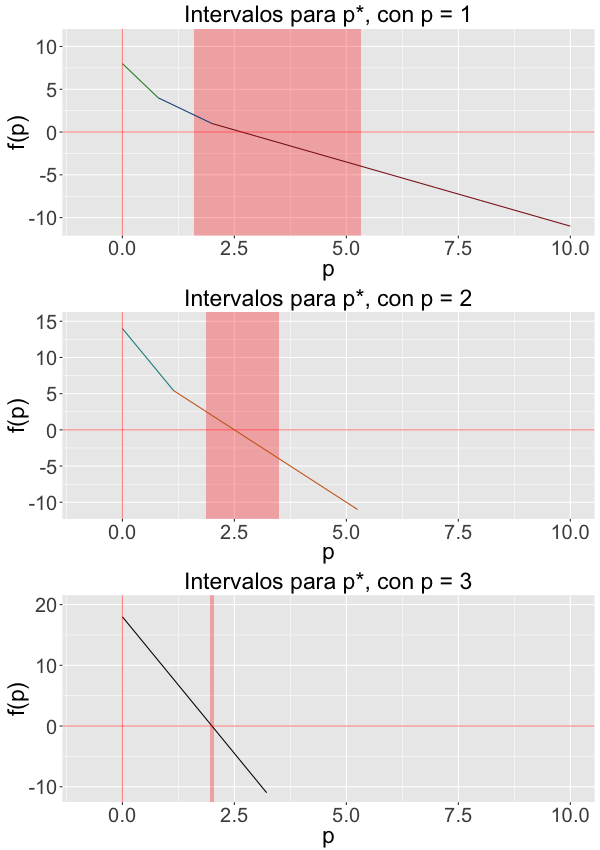
\includegraphics[width=.9 \textwidth]{Figures/Chapter2_grid3eigen_interv2}  
  \caption[Intervalos para $\rho^*$.] {La figura superior representa intervalos para $\rho^*$ cuando $f(\rho) = \lambda_{G(\rho)_1}$, la de enmedio cuando $f(\rho) = \lambda_{G(\rho)_1} + \lambda_{G(\rho)_2}$ y la de abajo cuando $f(\rho) = \lambda_{G(\rho)_1} + \lambda_{G(\rho)_2} + \lambda_{G(\rho)_3}$.}
\end{figure}




	%   \chapter{El Método Newton-Lanczos}
\label{ch:chapter3}
 
En el capítulo anterior se propuso una función no creciente $f(\rho)$ cuya raíz resulta ser la solución óptima para el problema del Discriminante Lineal de Fisher:

\begin{equation} \label{eq:3.1}
	f(\rho) = \max_{V^T V = I} Tr(V^T(S_E - \rho S_I)V)
\end{equation}

El algoritmo propuesto para encontrar la solución recibe el nombre de Newton-Lanczos\cite{ngo2012trace}. Para entenderlo a profundidad, se explicarán brevemente los métodos de Lanczos que tridiagonalizan una matriz simétrica, para después calcular eficientemente los primeros (últimos) eigenvalores. Después, será implementado junto al método iterativo de Newton, que calcula el nuevo valor de $\rho_{n}$ para cada paso. Para esto, se requiere el cómputo de la derivada de $f(\rho)$, por lo que se desarrollará su forma analítica. Finalizando, se proporcionarán las condiciones necesarias de optimalidad.

La primera división de los métodos para calcular eigenvectores y eigenvalores que propone J. Demmel \cite{demmel1997applied} depende si la matriz es simétrica o no lo es. Después hace una sub-clasificación dependiendo si el método es iterativo o directo. Para este texto solo se calcularán los eigenvalores de matrices simétricas, por lo que el procedimiento a seguir sera el siguiente:


\begin{itemize}
\item Tridiagonalizar la matriz simétrica por un método iterativo
\item Encontrar los eigenvalores por medio de la iteración tridiagonal QR (LAPACK DSTEVD)
\end{itemize}
\section{Métodos de Lanczos}
Antes de presentar los métodos de Lanczos, se dará una breve introducción acerca del costo computacional del algoritmo QR y la importancia de tridiagonalizar la matriz \cite{demmel1997applied}.  Sea $A \in {\rm I\!R}^{n \times n}$, entonces su descomposición $QR$ toma $O(n^3)$ flops. Suponiendo el mejor escenario en el que cada eigenvalor se encuentra con una iteración, tomaría $O(n^4)$ flops para calcular todos los eigenvalores de una matriz. Por otra parte, al tridiagonalizar la matriz $A$ se reduce el costo computacional de la descomposición $QR$ a $O(n^2)$ flops. De esta manera, tomaría $O(n^3)$ flops encontrar todos los eigenvalores. Una descripción más detallada del costo computacional de los algoritmos puede encontrarse en \cite{demmel1997applied}.

El primer paso, la tridiagonalización, ha sido muy estudiado y existen algoritmos especializados para distintos tipos de matrices simétricas. Si la matriz es de gran dimensión y rala, entonces se recomienda usar el método de Lanczos \cite{golub2012matrix}. En otro caso, existen las transformaciones Householder y las rotaciones de Givens \cite{golub2012matrix}. El método de Lanczos realiza tridiagonalizaciones parciales de la matriz original $A$, donde cada una es de tamaño $p \times p$ con $p\leq n$. Un aspecto interesante es que las matrices parciales van aproximando los eigenvectores extremos antes que la tridiagonalización esté completa. Por este motivo, el algoritmo es usado cuando se requieren solo algunos de los eigenvalores. Con respecto al costo computacional, es del orden $O(n^3)$, por lo que el algoritmo completo se mantiene en el mismo orden. 

Lanczos en aritmética exacta tiene muchas ventajas computacionales y converge rápidamente a los eigenvalores reales, pero con aritmética inexacta es difícil usarlo en la práctica \cite{golub2012matrix}. El problema que se presenta es que los eigenvectores van perdiendo la ortogonalidad entre ellos conforme la dimensionalidad y las iteraciones incrementan. Los textos \cite{demmel1997applied}\cite{golub2012matrix} incluyen algoritmos para solucionar este problema.

En la siguiente subsección se presentará el algoritmo original de Lanczos; se ejemplificará como los eigenvalores de la matriz tridiagonal convergen a los originales y se presenta el problema de \textit{ghost eigenvalues} \cite{demmel1997applied}, que son los eigenvalores que surgen al perder la ortogonalidad en aritmética inexacta.

\subsection{Algoritmo de Lanczos}

El algoritmo de Lanczos busca calcular los elementos de esta matriz tridiagonal directamente. Definiendo $Q^T A Q = T$, con $Q = [q_{(1)} \enskip|\enskip q_{(2)} \enskip|\enskip ... \enskip|\enskip q_{(n)}]$ ortogonal, y $T_n$ tridiagonal igual a:

\begin{equation}\label{eq:3.2}
T_n = \left(\!
    \begin{array}{cccccc}
      \alpha_1 & \beta_2 &  &  &  & 0\\
      \beta_2  & \alpha_2 & \beta_3 &  &  & \\
               & \beta_3 & \alpha_3 &  \ddots  & & \\
               &         & \ddots & \ddots & \beta_{n-1}& \\
               &  &  &  \beta_{n-1} & \alpha_{n-1} & \beta_n\\
       0       &  &  &  & \beta_n & \alpha_{n}\\
    \end{array}
  \!\right), \quad
\end{equation}

Como $q_{(1)}$ es una columna de Q, entonces $q_1^T = [q_{11},\enskip q_{21},\enskip ... ,\enskip q_{n1}]$. De esta manera, se tiene que $AQ = QT$. Descomponiendo la multiplicación $AQ =[Aq_{(1)} \enskip|\enskip Aq_{(2)} \enskip|\enskip ... \enskip|\enskip Aq_{(n)}]$ e igualándola a cada columna de $QT$, se tiene que $Aq_{(1)}$ \cite{golub2012matrix}:

\begin{equation*}
\begin{aligned}
Aq_{(1)} =\quad &  q_{(1)(1)} \alpha_{(1)}       &+\quad q_{(1)(2)} \beta_{(2)} \quad&+ \\
     & q_{(2)(1)}   \alpha_{(1)}       &+\quad q_{(2)(2)} \beta_{(2)} \quad&+ \\
     &          \qquad         \vdots&\vdots \qquad     & \\
     & q_{(n)(1)}   \alpha_{(1)}       &+\quad q_{(n)(2)} \beta_{(2)} \quad& \\
Aq_{(1)} =\quad & \alpha_{(1)} q_{(1)} &+\quad \beta_{(2)} q_{(2)}   \qquad& 
\end{aligned}
\end{equation*}

Ahora, para $i = 2, ..., n-1$
  
\begin{equation*}
\begin{aligned}
Aq_{(i)} =\quad &  q_{(i-1)(i-1)}\beta_{(i)}  &+ \enskip q_{(i-1)(i)}\alpha_{(i)} &+ \enskip q_{(i-1)(i+1)} \beta_{(i+1)} &+ \\
     & q_{(i)(i-1)}\beta_{(i)}       &+ \enskip q_{(i)(i)}\alpha_{(i)}\enskip   &+\enskip q_{(i)(i+1)} \beta_{(i+1)}   &+ \\
     & \vdots &          \qquad \qquad \quad \vdots & &\\
     & q_{(n)(i-1)}\beta_{(i)}      &+\enskip q_{(n)(i)}\alpha_{(i)} \enskip  &+\enskip q_{(n)(i+1)} \beta_{(i+1)}   & \\
Aq_{(i)} =\quad & \beta_{(i)} q_{(i-1)}      &+ \enskip\quad \alpha_{(i)} q_{(i)} \quad    &+\enskip \beta_{(i+1)} q_{(i+1)}      &
\end{aligned}
\end{equation*}

Por último, para $Aq_n$:

\begin{equation*}
\begin{aligned}
Aq_{(n)} =\quad &  q_{(1)(n)} \alpha_{(n)}       &+\quad q_{(1)(n-1)} \beta_{(n)} \quad&+ \\
     & q_{(2)(n)}   \alpha_{(n)}       &+\quad q_{(2)(n-1)} \beta_{(n)} \quad&+ \\
     &          \qquad         \vdots&\vdots \qquad     & \\
     & q_{(n)(n)}   \alpha_{(n)}       &+\quad q_{(n)(n-1)} \beta_{(n)} \quad& \\
Aq_{(n)} =\quad & \alpha_{(n)} q_{(n)} &+\quad \beta_{(n)} q_{(n-1)}   \qquad& 
\end{aligned}
\end{equation*}


Si se define $q_{(0)} = 0$, entonces se puede resumir el paso como:

\begin{equation}\label{eq:3.3}
  Aq_{(i)} = \beta_{(i)} q_{(i-1)} + \alpha_{(i)} q_{(i)}+ \beta_{(i+1)} q_{(i+1)}
\end{equation}

para $i = 1, .... n-1$. Multiplicando esta expresión por $q_{(i)}^T$, y usando el supuesto de ortogonalidad, entonces $q_{(i)}^T q_{(j)} = 0$ con $i \neq j$. De esta manera resulta la siguiente expresión:

\begin{equation}\label{eq:3.4}
\begin{aligned}
  q_{(i)}^TAq_{(i)} &=  q_{(i)}^T\alpha_{(i)} q_{(i)}  
                    &= \alpha_{(i)}
\end{aligned}
\end{equation}

Por otra parte, despejando $\beta_{(i+1)} q_{(i+1)}$ de \ref{eq:3.3}, se tiene que

\begin{equation}\label{eq:3.5}
\begin{aligned}
\beta_{(i+1)} q_{(i+1)}  =& Aq_{(i)} - \beta_{(i)} q_{(i-1)} - \alpha_{(i)} q_{(i)} \\ 
=& (A - \alpha_{(i)} I) q_{(i)} - \beta_{(i)} q_{(i-1)} = r_{(i)}
\end{aligned}
\end{equation}

Con la ecuación \ref{eq:3.5}, $q_{(i+1)} = \frac{r_{(i)}}{\beta_{(i+1)}}$. Calculando la norma de $r_{(i)}$, se tiene que 

\begin{equation}\label{eq:3.6}
\begin{aligned}
||r_{(i)}||_2 =& |\beta_{(i+1)}| ||q_{(i+1)}||_2 \\
              =& |\beta_{(i+1)}|
\end{aligned}
\end{equation}
 
Cuando $r_k =0$ entonces la iteración se detiene. \cite{golub2012matrix}

\pagebreak

\textbf{Implementación en aritmética exacta}\\

Sea $ A \in {\rm I\!R}^{n \times n}$ una matriz simétrica y $q_i \in {\rm I\!R}^{n}$. Entonces el algoritmo que se presenta a continuación produce una matriz $T_k \in {\rm I\!R}^{k \times k}$ tridiagonal tal que los eigenvalores de $T_k$ convergen a los de la matriz original $A$ \cite{golub2012matrix}. 

\begin{algorithm}[H] 
 $q_0$ $\leftarrow$ $0$\;
 $r_0$ $\leftarrow$ vector aleatorio\;
 $\beta_1$ $\leftarrow$ $||r_0||_2$\;
 $q_1 \leftarrow r_0 / \beta_1$\;
 $\alpha_1 \leftarrow q_1^T A q_1$\;
 $eps = 0.0000001$\;
 $k = 1$ \;
 \While{($\beta_k > eps$)}{
  $r_k \leftarrow A q_k - \alpha_k q_k - \beta_k q_{k-1}$\;
  $\beta_{k+1} \leftarrow ||r_{k-1}||_2$\;
  $q_{k+1} \leftarrow r_{k+1}/\beta{k+1}$\;
  $\alpha_{k+1} \leftarrow q_{k+1}^T A q_{k+1}$\;
  $k \leftarrow k+1$\;
 }
 \caption{Algoritmo de Lanczos}
\end{algorithm}

Para hacer frente a la pérdida de ortogonalidad entre los vectores, se han creado distintos métodos, los cuales se basan en la reortogonalización de la base de vectores. \cite{demmel1997applied} Esta puede realizarse en $O(n^2)$ operaciones, por lo que no afecta el orden de $O(n^3)$ flops.

\section{Derivada de $f(\rho)$}

La fórmula analítica de la derivada de $f(\rho)$ se puede obtener con cálculo multivariado. Para encontrarla, sea $V(\rho) \in {\rm I\!R}^{n \times p}$ una función diferenciable con respecto a $\rho$. Esta cumple la característica de ser una matriz ortogonal con columnas:

\begin{equation*}
	V(\rho) = (v_1(\rho) \enskip|\enskip v_2(\rho) \enskip|\enskip ... \enskip|\enskip v_p(\rho))
\end{equation*}

Antes de calcular la derivada de $f(\rho)$, es conveniente examinar la derivada de $V(\rho)^T V(\rho)$ con respecto a $\rho$. Sea $V(\rho)$ una matriz ortogonal; es decir, que cumpla $V^T(\rho) V(\rho) = I$, entonces \cite{ngo2012trace}:

\begin{equation*}
\frac{d}{d\rho} V(\rho)^T V(\rho) = \left(\frac{d}{d\rho}V(\rho)^T\right) V(\rho)  + V(\rho)^T 	\left( \frac{d}{d\rho} V(\rho) \right)
\end{equation*}

\vspace{5mm}

La derivada de $V(\rho)$ no se conoce explícitamente, pero se puede derivar componente a componente. De esta manera:


\begin{equation*}
\begin{aligned}
V(\rho)^T V(\rho)  &= \left(\!
    \begin{array}{cccc}
      v_{11}(\rho) & v_{21}(\rho) & \hdots & v_{n1}(\rho) \\
      v_{12}(\rho) & v_{22}(\rho) & \hdots & v_{n2}(\rho) \\
      \vdots & \vdots & \vdots & \vdots \\
      v_{1p}(\rho) & v_{2p}(\rho) & \hdots & v_{np}(\rho) 
    \end{array}
  \!\right)
    \left(\!
    \begin{array}{cccc}
      v_{11}(\rho) & v_{12}(\rho) & \hdots & v_{1p}(\rho) \\
      v_{21}(\rho) & v_{22}(\rho) & \hdots & v_{2p}(\rho) \\
      \vdots & \vdots & \vdots & \vdots \\
      v_{n1}(\rho) & v_{n2}(\rho) & \hdots & v_{np}(\rho) 
    \end{array} 
    \!\right) \\
    \vspace{5mm}
 &= \left(\!
    \begin{array}{c}
      v_{1}(\rho)^T \\
      v_{2}(\rho)^T \\
      \vdots \\
      v_{p}(\rho)^T  
    \end{array}
  \!\right)
  \left(\!
    \begin{array}{cccc}
      v_{1}(\rho) & v_{2}(\rho) & \hdots & v_{p}(\rho) 
    \end{array} 
	\!\right) 
\end{aligned}
\end{equation*}

Entonces la entrada $(i,j)$ de $V(\rho)^T V(\rho)$ es:

\begin{equation*}
	[V(\rho)^T V(\rho)]_{ij} = v_i(\rho)^T v_j(\rho)
\end{equation*}

Calculando la derivada:

\begin{equation*}
\frac{d}{d\rho}[V(\rho)^T V(\rho)]_{ij} =  \left( \frac{d}{d\rho}v_i(\rho)^T \right)  v_j(\rho) + v_i(\rho)^T \left( \frac{d}{d\rho} v_j(\rho)\right) 
\end{equation*}

En específico para el caso $i = j$:
\vspace{5mm}
\begin{equation}\label{eq:3.7}
\frac{d}{d\rho}[V(\rho)^T V(\rho)]_{ii} =  2 \left( \frac{d}{d\rho}v_i(\rho)^T \right)  v_i(\rho)
\end{equation}

\bigskip

\begin{lemma}\label{lemma:3.1}
Sea $V(\rho) \in {\rm I\!R}^{n \times p}$ una matriz ortogonal y $\rho$ su parámetro. Entonces \cite{ngo2012trace}:
\begin{equation*}
\begin{aligned}
(i)&  \quad \frac{d}{d\rho} V(\rho)^TV(\rho) = \left(\frac{d}{d\rho}V(\rho)^T\right) V(\rho)  + V(\rho)^T  \left( \frac{d}{d\rho} V(\rho) \right) = 0 \\
(ii)& \quad Diag \left(\left(\frac{d}{d\rho}V^T \right)V(\rho) \right) = 0 
\end{aligned}
\end{equation*}
\end{lemma}

\begin{proof}
\bigskip
(i) Para demostrar la primer propiedad se hace uso de que $V(\rho)^T V(\rho) = I_p$, entonces:
\begin{equation*}
\frac{d}{d\rho} [V(\rho)^T V(\rho)] = 0  
\end{equation*}

(ii) Se parte de la ecuación (\ref{eq:3.7}), y se usa el punto (i):
\begin{equation*}
  \frac{d}{d\rho} [V(\rho)^T V(\rho)]_{ii} =    2 \left( \frac{d}{d\rho}v_i(\rho)^T \right)  v_i(\rho) = 0
\end{equation*}

Como cada elemento $i$ es cero, entonces en particular $Diag\left( \left(\frac{d}{d\rho}V(\rho)^T \right) V(\rho) \right)=0 $.
\end{proof}

Del lema \ref{lemma:3.1} se tiene que $\left(\frac{d}{d\rho}V(\rho)^T \right) V(\rho)$ tiene diagonal igual a 0. Ahora, para derivar $f(\rho)$, primero se deriva la expresión $\frac{d}{d\rho}\left[V^T (A-\rho B)V \right]$:

\begin{equation}\label{eq:3.8}
\begin{aligned}
	\frac{d}{d\rho}\left[V^T (A-\rho B)V \right] & = \frac{d}{d\rho} \left[V^T A V \right]- \frac{d}{d\rho}\left[V^T \rho B V\right] \\
	& = \frac{dV^T}{d\rho}  AV +  V^T A \frac{dV}{d\rho} - \frac{dV^T}{d\rho} \rho BV - V^T \left[BV + \rho B \left(\frac{dV}{d\rho} \right) \right] \\
	& = \frac{dV^T}{d\rho} \left[A -\rho B \right] V + V^T \left[A- \rho B \right]\frac{dV}{d\rho} - V^TBV \\
\end{aligned} 
\end{equation}


Sea $V$ la matriz que diagonaliza $(A-\rho B)$, de manera que $V^T (A-\rho B) V = D$. Entonces \ref{eq:3.8}:
\begin{equation}\label{eq:3.9}
\begin{aligned}
\frac{d}{d\rho}\left[V^T (A-\rho B)V \right] & = \frac{dV^T}{d\rho} VD  + DV^T\frac{dV}{d\rho} - V^TBV 
\end{aligned}
\end{equation}

Al calcular la traza de (\ref{eq:3.9}) y usando del lema \ref{lemma:3.1}, se tiene que:
\begin{equation}\label{eq:3.10}
\begin{aligned}
Tr\left[\frac{d}{d\rho} \left[V^T (A-\rho B)V \right]\right] & = Tr\left[ \frac{dV^T}{d\rho} VD + DV^T \frac{dV}{d\rho} - V^T B V  \right] \\
											     & = 2 Tr \left[ D V^T \frac{dV}{d\rho} \right] - Tr \left[ V^T B V \right] \\
											     & = -Tr\left[V^T B V \right] 
\end{aligned}	
\end{equation}

\section{Método Newton-Lanczos}

El método de Newton establece que la iteración está dada por:

\begin{equation*}
x_{(n+1)} = x_{(n)} - \frac{f(x_n)}{f'(x_n)}
\end{equation*}

con $f'(x_n)$ la derivada de $f(x_n)$.

Con esta fórmula y con (\ref{eq:3.10}), se puede calcular explícitamente $\rho_{n+1}$ para la iteración de Lanczos \cite{ngo2012trace}:

\begin{equation}\label{eq:3.11}
\begin{aligned}
\rho_{n+1} =& \rho_{n} - \frac{Tr\left[V^T (A-\rho_n B)V \right]}{-Tr\left[V^T B V \right]} \\ \\
           =& \frac{\rho_{n} Tr\left[V^T B V \right] +  Tr\left[V^T (A-\rho_n B)V \right]}{Tr\left[V^T B V \right]}\\ \\
           =& \frac{\rho_{n} Tr\left[V^T B V \right] +  Tr\left[V^T A V \right] - \rho_nTr\left[V^T BV \right]}{Tr\left[V^T B V \right]} \\ \\
           =&\frac{Tr\left[V^T A V \right]}{Tr\left[V^T B V \right]}
\end{aligned} 
\end{equation}

Una vez calculado el paso de la iteración, se enuncia el método de Newton-Lanczos para maximizar el cociente de trazas. El método recibe como entrada la matriz $A$, $B$ y la dimensión a la cual se desea proyectar $p$ \cite{ngo2012trace}: 

\begin{algorithm}[H]
i = 1\;
$\rho_1$ un número aleatorio\;
$\rho_0$\;
$f(\rho_1) = \sum\limits_{j = 1}^{p} \lambda_{(A-\rho_1 B)_j}$\;
V = primeros $p$ eigenvectores de $A-\rho_1 B$\;
$tol = 1e-10$\;

\While{($i<50$ \quad , \quad $abs(\rho_i-\rho_{i-1}$)$>tol$)}{
$i = i+1$\;
V = primeros $p$ eigenvectores de $(A-\rho_i B)$ \;
$\rho_i = Tr(V^T A V)/Tr(V^T BV)$\;
$f(\rho_i) = \sum\limits_{j = 1}^{p} \lambda_{(A-\rho_i B)_j}$\;
}
 \caption{Algoritmo de Newton-Lanczos}
\end{algorithm}


\subsection{Condiciones necesarias de optimalidad}
Considerando el problema de maximizar las trazas:

\begin{equation}\label{eq:3.12}
  \max_{\substack{V \in {\rm I\!R}^{n \times p} \\ V^TV = I}} \frac{Tr(V^T S_E V)}{Tr(V^T S_I V)} 
\end{equation}

La función lagrangiana asociada a este problema es la siguiente \cite{ngo2012trace}:

\begin{equation*}
L(V, \Gamma) =  \frac{Tr(V^T S_E V)}{Tr(V^T S_I V)} - Tr[\Gamma(V^TV-I)]
\end{equation*}

Con $\Gamma \in {\rm I\!R}^{p \times p}$ , la matriz de multiplicadores de Lagrange de la forma:

\begin{equation*}
\Gamma = \left(\!
    \begin{array}{ccccc}
    \gamma_{(1)(1)} & \gamma_{(1)(2)} & \hdots & \gamma_{(1)(p-1)} & \gamma_{(1)(p)} \\
    \gamma_{(2)(1)} & \gamma_{(2)(2)} & \hdots & \gamma_{(2)(p-1)} & \gamma_{(2)(p)} \\
    \vdots & \vdots & \vdots & \vdots & \vdots \\
    \gamma_{(p-1)(1)} & \gamma_{(p-1)(2)} & \hdots & \gamma_{(p-1)(p-1)} & \gamma_{(p-1)(p)} \\
    \gamma_{(p)(1)} & \gamma_{(p)(2)} & \hdots & \gamma_{(p)(p-1)} & \gamma_{(p)(p)} \\
\end{array}
  \!\right), \quad
\end{equation*}


Ya que al multiplicar esta matriz por $[V^T V- I]$ (con $V = (v_1 \enskip |\enskip v_2 \enskip |\enskip ... \enskip |\enskip v_{p-1} \enskip |\enskip v_p)$) se tiene que: 

\begin{equation*}
V^T V - I = \left(\!
    \begin{array}{ccccc}
    v_1^T v_1 -1& v_1^T v_2 & \hdots & v_1^T v_{p-1} & v_1^T v_p \\
    v_2^T v_1 & v_2^T v_2 -1& \hdots & v_2^T v_{p-1} & v_2^T v_p \\
    \vdots & \vdots & \vdots & \vdots & \vdots \\
    v_{p-1}^T v_1 & v_{p-1}^T v_2 & \hdots & v_{p-1}^T v_{p-1} -1& v_{p-1}^Tv_p \\
    v_p^T v_1 & v_p^T v_2 & \hdots & v_p^Tv_{p-1} & v_{p}^Tv_{p} -1 \\
\end{array}
  \!\right), \quad
\end{equation*}

entonces, la diagonal de ($\Gamma (V^T V - I)$) contiene $p$ elementos que son los siguientes: 

\begin{equation*}
\left(\!
    \begin{array}{c}
    \begin{aligned}
    & \gamma_{(1)(1)}(v_1^T v_1 -1) &+& \gamma_{(1)(2)} (v_2^T v_1) &+& \hdots &+& \gamma_{(1)(p)}(v_p^T v_1) &\\
    & \gamma_{(2)(1)}(v_1^T v_2) &+& \gamma_{(2)(2)}(v_2^T v_2 -1)  &+& \hdots &+& \gamma_{(2)(p)}(v_p^T v_2) &\\
    & \vdots && \vdots && \vdots && \vdots &\\
    &\gamma_{(p-1)(1)}(v_1^T v_{p-1}) &+& \gamma_{(p-1)(2)} (v_2^T v_{p-1}) &+& \hdots &+& \gamma_{(p-1)(p)}(v_p^T v_{p-1})&\\
    &\gamma_{(p)(1)}(v_1^T v_{p}) &+& \gamma_{(p)(2)}(v_2^T v_p)  &+& \hdots &+& \gamma_{(p)(p)}(v_p^T v_{p}-1) &\\
\end{aligned}
\end{array}
  \!\right), \quad
\end{equation*}

Para calcular la traza se suman estos elementos de la diagonal. De esta forma, se tienen p restricciones de la forma $v_i^T v_i = 1 \quad i = 1,...,p$ y $p(p-1)$ restricciones de la 
forma $v_i^T v_j = 0 \quad i \neq j, \quad i,j = 1, ..., p$, cada una con su multiplicador lagrangiano.

Como la ecuación a maximizar tiene un maximizador global $V^*$, entonces existe un multiplicador matricial lagrangiano tal que en el óptimo:

\begin{equation}\label{eq:3.13}
\frac{\partial \mathcal{L}(V^*, \Gamma^*)}{\partial V} =  0 \qquad con \qquad V^{T*}V^* = I
\end{equation}

Para encontrar $(V^*, \Gamma^*)$ de (\ref{eq:3.13}), primero se debe conocer la derivada de $\frac{\partial Tr(V^T M V)}{\partial V}$, con M cualquier matriz:

\begin{equation}\label{eq:3.14}
\frac{\partial Tr(V^T M V)}{\partial V} = (M^* +M)V  
\end{equation}

\pagebreak
Derivando el lagrangiano (\ref{eq:3.13}) y utilizando (\ref{eq:3.14}) se tiene que:

\begin{equation*}
\begin{aligned}
\frac{\partial \mathcal{L}(V, \Gamma)}{\partial V} =&\quad  \left[\frac{\partial Tr(V^T A V) }{\partial V}\right]\left[Tr(V^T B V)^{-1}\right] \quad +& \\
&\quad \left[Tr(V^T A V)\right]\left[\frac{\partial (Tr(V^T B V))^{-1} }{\partial V}\right] \quad -& \\
&\quad \left[\frac{\partial Tr[\Gamma(V^TV-I)] }{\partial V}\right] \quad &
\end{aligned}
\end{equation*}
\vspace{5mm}

\begin{equation*}
\begin{aligned}
\frac{\partial \mathcal{L}(V, \Gamma)}{\partial V} =&\quad  \left[2AV\right]\left[Tr(V^T B V)^{-1}\right] \quad +& \\
&\quad \left[Tr(V^T A V)\right]\left[\frac{2BV}{Tr(V^T B V)^2}\right] \quad -& \\
&\quad \left[V (\Gamma^* + \Gamma) \right] \quad &
\end{aligned}
\end{equation*}
\vspace{5mm}

\begin{equation}\label{eq:3.15}
\begin{aligned}
\frac{\partial \mathcal{L}(V, \Gamma)}{\partial V} =&\quad  \left[\frac{2AV Tr(V^T B V)- 2BV Tr(V^T A V)}{(Tr(V^T B V))^2}\right] \quad +& \\
&\quad \left[V (\Gamma^* + \Gamma) \right] \quad &
\end{aligned}
\end{equation}

Igualando (\ref{eq:3.15}) a cero y acomodando la expresión, resulta:
\begin{equation*}
\left[A-\frac{Tr(V^{T*} A V^*)}{Tr(V^{T*} B V^*)}B\right] V^*  = \left[\frac{Tr(V^{T*} B V^*)}{2}V^* (\Gamma^{T*} + \Gamma^{*})\right]
\end{equation*}

\begin{equation}\label{eq:3.16}
\left[ A-\rho^* B\right]V^*   = \left[ \frac{Tr(V^{T*} B V^*)}{2}V^* (\Gamma^{T*} + \Gamma^{*}) \right]
\end{equation}

Con $\rho^* = \frac{Tr(V^{T*} A V^*)}{Tr(V^{T*} B V^*)}$. Sea $Q$ la matriz ortogonal que diagonaliza $\Gamma^{T*} + \Gamma^{*}$, entonces se puede escribir la expresión $(\Gamma^{T*} + \Gamma^*)$ como:
\begin{equation*}
 \left(\Gamma^{T*} + \Gamma^{*}\right) = Q \Sigma^* Q^T \qquad con \qquad Q^TQ = I
\end{equation*}

Con $\Sigma^*$ una matriz diagonal. Multiplicando (\ref{eq:3.16}) por $V^{T*}$ y calculando la traza de ambos lados de la ecuación y se tiene que:

\begin{equation*}
\begin{aligned}
Tr\left[ V^{T*}(A-\rho^* B)V^*\right]  =& \left[ \frac{Tr(V^{T*} B V^*)}{2}\right] Tr(\Gamma^{T*} + \Gamma^{*}) \\ \\
Tr(\Gamma^{T*} + \Gamma^{*}) =& 2 \frac{Tr(V^{T*}(A-\rho^*B)V^*)}{Tr(V^{T*}BV^*)} = 0 
\end{aligned}
\end{equation*}
\vspace{5mm}
\begin{equation}\label{eq:3.17}
Tr(Q \Sigma^* Q^T) = 2 \frac{Tr(V^{T*}(A-\rho^*B)V^*)}{Tr(V^{T*}BV^*)} = 0
\end{equation}


Como $Tr(V^{T*}(A-\rho^*B)V^*) = 0$ entonces $Tr(Q \Sigma^* Q^T) =0$, por lo que $Tr(\Sigma^*) = 0$. Definiendo $U^* = V^*Q$, con $U^*U = I$, la expresión (\ref{eq:3.16}) se puede escribir como:

\begin{equation*}
\begin{aligned}
\left[ A-\rho^* B\right]V^*   &= \left[ \frac{Tr(V^{T*} B V^*)}{2}V^* (Q \Sigma^* Q^T) \right] \\\\
                              &= \left[ \frac{Tr(V^{T*} B V^*)}{2}U^*Q^{T*} (Q \Sigma^* Q^T) Q \right] \\\\
                              &= \left[ \frac{Tr(V^{T*} B V^*)}{2}U^* \Sigma^* \right] \\
\end{aligned}
\end{equation*}  

Definiendo $\Lambda_* = \frac{Tr(V^{T*} B V^*)}{2}\Sigma^*$, entonces:
\begin{equation}\label{eq:3.18}
\begin{aligned}
\left[ A-\rho^* B\right]U^*   &= U^* \Lambda_* \\
 U^{T*} \left(A-\rho^* B\right)U^*   &=  \Lambda_* \\
 Tr(U^{T*} \left(A-\rho^* B\right)U^*)   &=  Tr(\Lambda_*) = 0
\end{aligned}
\end{equation}  

De esta manera se tiene que la ecuación (\ref{eq:3.18}) es la condición necesaria para que $U^*, \rho^*$ sean las óptimas










	%   \chapter{Experimentos numéricos}
\label{ch:chapter4}

Para medir el desempeño del algoritmo Newton-Lanczos se compara con otros dos métodos, el Análisis Discriminante Lineal (ADL) y la Regresión Logística Multinomial (RLM). Los criterios para elegir el mejor serán la tasa de reconocimiento y el tiempo de cómputo sobre los conjuntos de datos JAFFE y MNIST. Como el algoritmo de Newton-Lanczos ocupa los eigenvectores de una matriz, en la primer parte de este capítulo se medirá el tiempo de Lanczos y el costo de la rutina $SVD$ de R para una matriz en particular \footnote{La rutina $svd$ de $R$ ocupa la función $gesdd$ de la librería $LAPACK$. Para más información puede consultarse la página $http://www.netlib.org/lapack/$.}. En la segunda parte del capítulo, se explicará el preprocesamiento de las bases de datos y como se crearon los conjuntos de entrenamiento y prueba. En la tercer y cuarta parte, se realizan los experimentos con la bases de MNIST y JAFFE respectivamente. 

Para todos los experimentos de este capítulo, se utilizó el lenguaje de \textsf{R} en su versión 3.2.2 \textit{Fire Safety}. Los cálculos fueron realizados en una iMac 3.2 Ghz Intel Core i3 con 12 GB de RAM.

\section{Desempeño del método de Lanczos}

Antes de analizar el tiempo de cómputo de Newton-Lanczos, se evaluará el desempeño del algoritmo de Lanczos comparándolo con la factorización $svd$. Esto experimento es para saber en que casos es conveniente utilizar Lanczos y en cuales conviene calcular todos eigenpares. Para la prueba se usó $A - \rho B$ con $A$ y $B$ las matrices de dispersión intra clase y entre clase de la base de datos MNIST y con $\rho = 3$. La figura \ref{fig5.1} resume el desempeño de ambos métodos.

\begin{figure}[!ht] \label{fig5.1}
  \centering
  \includegraphics[width=1\textwidth]{Figures/Chapter4_eigen_lanczos.png} 
  \caption[Desempeño de Lanczos.] {Desempeño de Lanczos. En el eje $x$ se representa k, el número de eigenpares a calcular de la matriz $A- \rho B$. La matriz original es de 193 x 193. El tiempo reportado para cada $k$, es el promedio de $30$ repeticiones para cada método.}
\end{figure}

Se observa que, para $k$ menor a 10, el algoritmo de Lanczos es más rápido que la factorización $SVD$ de la matriz completa. Para valores más grandes, conviene factorizar toda la matriz. Esto puede deberse a que en aritmética inexacta Lanczos presenta el problema de \textit{Ghost eigenvalues} (eigenvalores que se repiten, pero que son espurios) \cite{golub2012matrix}. Estos se originan porque la ortogonalidad entre los eigenvectores se pierde conforme la dimensionalidad aumenta. Para solucionar este problema, se tuvo que realizar una reortogonalización completa en cada iteración, lo que pudo aumentar el tiempo de cómputo. 

\section{Modelos comparados y preprocesamiento de las bases}

En este capítulo, el método de Newton-Lanczos se comparó otros dos métodos de clasificación: la RLM y con el ADL. Para el primero, se usó la función \textit{multinom} del paquete \textit{nnet}, mientras que para el segundo se utilizó una modificación de la función \textit{lda} \footnote{La modificación está presentada en los códigos del apéndice B} del paquete \textit{MASS}. Ambas funciones fueron desarrolladas por Brian Ripley, profesor de estadística aplicada de la Universidad de Oxford. 

Como primer paso, se definieron los tamaños del conjunto de entrenamiento y prueba. Para el entrenamiento de MNIST se ocuparon 4000 datos (400 por clase); es decir, el 6\% del total. En el caso de JAFFE se utilizaron 50 datos (5 por clase); es decir, el 23\% del total. En ambos, el resto de los datos se ocupó en el conjunto de prueba. 

Para el preprocesamiento de las bases, cada imagen se convirtió en un vector con tamaño asociado al número de píxeles. Esto genera un problema de dimensionalidad, por lo que se realizó un paso de reducción dimensional. Se tomaron las primeras componentes principales (PCA) del conjunto de entrenamiento de manera que se explicara el 95\% de la varianza total, después se proyectó el conjunto de prueba. (De esta manera, los individuos en lugar de pertenecer a un espacio de ${\rm I\!R}^{m \times n}$, pertenecen a uno menor). Para MNIST se tomaron 193 de las 784 componentes; en cambio, para JAFFE solo 50 de las 65536. 

Una vez hecho el preprocesamiento, se realizaron 2 experimentos para cada base de datos. En el primero se utilizó el método de Newton-Lanczos con $V \in {\rm I\!R}^{m \times 20}$. Después de esto se proyectaron a los individuos originales a un espacio 20-dimensional. Los objetivos fueron los siguientes: 

\begin{itemize}
\item Analizar como cambia el valor de $f(\rho)$ con el método de Newton-Lanczos
\item Ver como se ven proyectados los datos en dimensiones menores
\end{itemize}

En el segundo experimento se entrenaron los 3 métodos con distintas $p$. Después se midió la tasa de reconocimiento alcanzada (usando el conjunto de prueba) y su tiempo de ejecución. 

\section{Base de datos MNIST}

Las siglas MNIST provienen de (\textit{Mixed National Institute of Standards and Technology}), la cual contiene datos de 70,000 dígitos escritos a mano que se usan comúnmente para probar códigos de clasificación de imágenes. De esta manera, en el experimento se tendrán 10 clases: los dígitos del 0-10. La base de datos surge de la colaboración de Yann LeCun del Instituto Courant (NYU), de Corinna Cortes de Google Labs (NY) y de Christopher J.C. Burges de Microsoft Research en Redmond. Puede descargarse de la página Web \textit{yann.lecun.com/exdb/mnist}, cuyo link sigue vigente al 13 de marzo del 2016.

Las imágenes están en un formato especial llamado IDX. Para poderlas convertir en un archivo leíble para R, se utilizó la función \textit{readMNIST} del paquete \textit{darch}. Esta paquetería convierte los archivos a objetos \textit{.RData}. La figura 3.2 contiene una extracto de tamaño 225 de todo el conjunto.

\begin{figure}[!ht]\label{fig5.2}
  \centering
	\includegraphics[width=1\textwidth]{Figures/Chapter4_numeros.png}	
  \caption{Ejemplo de números de la base de datos (MNIST).}
\end{figure}

\subsection{Proyección sobre un espacio de dimensión 20}

\underline{\textbf{1) Cotas para $\rho^*$}}

En el capítulo 2 se presentaron cotas para $\rho^*$ y en esta sección se ejemplificará la segunda de ellas para esta base de datos. Se calcularon los eigenvalores de la matriz intraclase (B) y de la matriz entre clases (A). Los 20 eigenvalores más grandes y más pequeños de la primera son \footnote{los eigenvalores menores a $1e^{-10}$ se consideraron numéricamente como 0}:

\begin{center}
\begin{tabular}{ | c | c|  c |c | c|  c |c | c|  c |c | c | c|  c |c | c|  c |c | c|  c |c |} 
\hline
12694 & 10367 & 7822 & 6793 & 6013 & 5887 & 5269 & 4704 & 4474 & 3969 \\
3833 & 3428 & 3124 & 3015 & 2978 & 2627 & 2535 & 2353 & 2232 & 2150 \\
\hline
\hline
\end{tabular}
\end{center}

\begin{center}
\begin{tabular}{ | c | c|  c |c | c|  c |c | c|  c |c | c | c|  c |c | c|  c |c | c|  c |c |} 
\hline
73 & 72 & 72 & 71 & 71 & 70 & 70 & 69 & 68 & 68 \\
67 & 67 & 66 & 66 & 65 & 64 & 64 & 63 & 63 & 62 \\
\hline
\hline
\end{tabular}
\end{center}

Mientras que los 9 eigenvalores más grandes de la matriz entre clases (A) son (los demás son 0):

\begin{center}
\begin{tabular}{ | c | c|  c |c | c|  c |c | c|  c |} 
\hline
12865 & 9821 & 7408 & 4736 & 3558 & 2312 & 1879 & 885 & 631 \\
\hline
\hline
\end{tabular}
\end{center}

Sustituyendo estos valores en la fórmula de las cotas de la raíz, se tiene que:

\begin{equation*}
\frac{\sum_{i = 1}^{p}\lambda_{A_i}}{\sum_{i = 1}^{p}\lambda_{B_i}} \leq \rho^* \leq \frac{\sum_{i = 1}^{p}\lambda_{(A)_i}}{\sum_{i = 1}^{p}\lambda_{(B)_{n-i+1}}}	
\end{equation*}

\begin{equation*}
\frac{44099.28}{96277.31} \leq \rho^* \leq \frac{44099.28}{1364.54}
\end{equation*}

\begin{equation*}
0.4580443 \leq \rho^* \leq 32.31806
\end{equation*}

A continuación se presentan como se ven $(\rho^*, f(\rho))$ con cada iteración para el método de Newton-Lanczos. 

\pagebreak

\underline{\textbf{2) Valores de $(\rho^*, f(\rho))$}}

Para el punto inicial de este experimento se utilizará el punto medio del intervalo. Los criterios de paro se fijaron con una tolerancia de $1e^{-10}$ y que las iteraciones sean menor a 50. Con este ejemplo, se obtienen los siguientes resultados para $\rho$ y $f(\rho)$:

\begin{center}
\begin{tabular}{ | c | c|  c |} 
\hline
$iter$ & $\rho$ & $f(\rho)$  \\ 
\hline
\hline
1 & $16.38805180$ & $-22,326.51$  \\ 
\hline
2 & $0.03121373$ & $42,841.16$  \\ 
\hline
3 & $1.11003833$ & $15,197.50$  \\ 
\hline
4 & $2.05957127$ & $3,926.463$  \\ 
\hline
5 & $2.50843464$ & $444.8128$  \\ 
\hline
6 & $2.57388828$ & $9.007894$  \\ 
\hline
7 & $2.57526971$ & $.004008613$  \\ 
\hline
8 & $2.57527033$ & $7.891856e^{-10}$  \\ 
\hline
9 & $2.57527033$ & $5.371703e^{-12}$  \\ 
\hline
\hline

\end{tabular}
\end{center}

\begin{figure}[!ht] \label{fig5.3}
  \centering
	\includegraphics[width=.75\textwidth]{Figures/Chapter4_Iteraciones.png}	
  \caption[Valores de $\rho$ y $f(\rho)$ para distintas iteraciones (MNIST).] 
  {Valores de $\rho$ y $f(\rho)$ para distintas iteraciones (MNIST). El punto rojo es el punto inicial. Datos del conjunto de entrenamiento.}
\end{figure}

En la figura 3.3 se muestran $(\rho, f(\rho))$ para cada una de las 9 iteraciones. El punto inicial es el rojo, en este caso $\rho = 16.39$, mientras que $f(\rho)$ toma el valor de $-22,326$. Tras la primer iteración, $\rho$ toma el valor de $0.03$, y $f(\rho)$ es igual $42,841$. Conforme hay más iteraciones, $\rho$ y $f(\rho)$ convergen a los óptimos.

\underline{\textbf{3) Datos proyectados en 4 dimensiones}}

Se maximizó la traza del cociente para un espacio de 20 dimensiones. En la figura 3.4 se muestra como se agrupan los individuos del conjunto de entrenamiento conforme las iteraciones avanzan. 
  
\begin{figure}[!ht] \label{fig5.4}
  \centering
	\includegraphics[width=1\textwidth]{Figures/Chapter4_ejemplo20componentes.png}	
  \caption[Ejemplo de proyección en 20 dimensiones (MNIST).]
  {Ejemplo de proyección en 20 dimensiones (MNIST). Las dos imágenes superiores son los datos de entrenamiento proyectadas sobre las 4 primeras componentes tras la primer iteración. Las dos intermedias son en la iteración 3 y las últimas 2 son la última iteración. Datos del conjunto de entrenamiento.}
\end{figure}

\subsection{Comparación con otros métodos}

Para la comparación de Newton-Lanczos con la RLM y el ADL se tomaron las siguientes consideraciones:

\begin{itemize}
\item Las dimensiones a considerar (k) son: 2, 5, 10, 15, 20, 40, 60, 80, 100, 120, 140, 160, 180 y 193
\item El número de variables que entran en cada modelo es el mismo (dada la dimensión k)
\item Los modelos se ajustan con el conjunto de entrenamiento y se calcula el error con el de prueba
\item Para Newton-Lanczos y ADL se proyectarán a un espacio k-dimensional y se usará 3-vecinos más cercanos para clasificarlos
\item Para el caso de regresión logística multinomial se elegirá la clase que tenga una mayor probabilidad posterior de selección
\end{itemize}

\underline{\textbf{1) Tasa de reconocimiento}}

La tasa de reconocimiento se mide como el número de individuos clasificados correctamente entre el número total del conjunto de test. Como el objetivo de esta sección es observar como se modifica la tasa con respecto aumenta k, se fijó el número de vecinos más cercanos a 3 para el caso de ADL y de Newton-Lanczos y también el tamaño del conjunto de entrenamiento. En la figura 3.5 se muestra que el modelo RLM y el ADL se comportan mejor para dimensiones pequeñas. Para casos de k mayor a 120, el método de Newton-Lanczos alcanza una mejor tasa de reconocimiento.

Es interesante observar que si se busca la mejor proyección con para k = 1 y k = 2, Newton-Lanczos resulta ser muy buen método. En la 3.4 se observó como los individuos se agrupan con este método. 


\begin{figure}[!ht] \label{fig5.5}
  \centering
	\includegraphics[width=1\textwidth]{Figures/Chapter4_Comparacion.png}	
  \caption[Tasa de reconocimiento base (MNIST).]
  {Tasa de reconocimiento base (MNIST). En azul se representa el RLM, en verde el ADL y en rojo el método de Newton-Lanczos. En el eje $y$ se muestra la tasa de reconocimiento y en el eje $x$ la dimensión a considerar (k). El tamaño representa el tiempo. Datos del conjunto de prueba.}
\end{figure}

\pagebreak
\underline{\textbf{2) Tiempo de ejecución}}

A continuación, se comparan los tiempos de ejecución de cada método. Para comparar los tiempos de ejecución justamente, se tomaron 3 distintos:

\begin{itemize}
\item 1) (PCA) Tiempo para calcular los componentes principales del conjunto de entrenamiento
\item 2) (Proyectar) Tiempo para calcular la proyección del conjunto de test
\item 3) (Modelo) Tiempo necesario para hacer las operaciones de cada método

\end{itemize}

\begin{center}
\begin{tabular}{ | c | c |} 
\hline
 PCA(s) & Proyectar(s) \\ 
\hline
\hline
$11.728$ & $21.680$ \\ 
\hline
\hline
\end{tabular}
\end{center}

La siguiente tabla muestra los tiempos de cómputo para los 3 métodos y con distinto número de componentes. 

\begin{center}
\begin{tabular}{ | c | c | c | c ||| c | c | c | c |} 
\hline
Comp & lda.iter & logístico & lda.orig   & Comp & lda.iter & logístico & lda.orig   \\ 
\hline
\hline
$2$ & $0.9092$ & $0.2712$ & $0.01$ & $80$ & $0.9222$ & $4.3186$ & $0.2684$ \\
$5$ & $0.8576$ & $0.5188$ & $0.0466$ & $100$ & $0.8764$ & $5.6474$ & $0.3572$ \\
$10$ & $0.864$ & $1.0646$ & $0.025$ & $120$ & $0.8952$ & $8.1026$ & $0.4942$ \\
$15$ & $0.8768$ & $1.103$ & $0.0372$ & $140$ & $0.9016$ & $9.2944$ & $0.7902$ \\
$20$ & $0.8886$ & $1.2888$ & $0.0524$ & $160$ & $0.8782$ & $10.1534$ & $0.908$ \\
$40$ & $0.886$ & $2.5528$ & $0.1004$ & $180$ & $0.898$ & $12.0426$ & $1.0596$ \\
$60$ & $0.8728$ & $3.2034$ & $0.1744$ & $193$ & $0643$ & $14.2512$ & $1.2186$ \\
\hline
\hline
\end{tabular}
\end{center}

El tiempo está en segundos (s).

Para cada iteración del método de Newton-Lanczos, se calcularon todos los eigenvalores ya que al no calcularlos, solo se tendrá una aproximación a sus valores y sus eigenvectores. Por este motivo, se decidió sacrificar tiempo de cómputo por precisión.

\pagebreak
\section{Base de datos JAFFE}


Ahora se analizará la base JAFFE \textit{Japanese Female Facial Expression}, que consta de 213 fotos provenientes de 10 personas distintas. Este conjunto de datos fue creado inicialmente para clasificar emociones, pero se usa comúnmente para probar otros tipos de algoritmos de clasificación. En nuestro caso será usado para clasificar el rostro de la persona, de esta manera se tendrán 10 clases. La base fue creada por Michael Lyons, Miyuki Kamachi y Jiro Gyoba en el departamento de psicología de la universidad de Kyushu. Puede descargarse de la página Web \textit{www.kasrl.org/jaffe.html}, cuyo link sigue vigente al 13 de marzo del 2016.

Las imágenes se encuentran en un formato \textit{.tiff}, por lo que se requirió la función \textit{readTIFF} del paquete $tiff$ el cual permite leerlas y convertirlas en un formato \textit{.RData}. La figura 3.6 contiene un extracto de tamaño 35 de la base original.

\begin{figure}[!ht]
  \centering
  \includegraphics[width=.8\textwidth]{Figures/Chapter4_Jaffe.png} 
  \caption{Ejemplo de la base de datos (JAFFE).}
\end{figure}

\pagebreak
\subsection{Proyección sobre un espacio de dimensión 20}

\underline{\textbf{1) Cotas para $\rho^*$}}

Al igual que el ejemplo de MNIST, se ejemplificará la segunda cota presentada en el capítulo 2. Para esto se calcularon los eigenvalores de la matriz intraclase (B) y de la matriz entre clases (A). Los 20 eigenvalores más grandes y más pequeños de la primera son: \footnote{los eigenvalores menores a $1e^{-10}$ se consideraron numéricamente como 0}

\begin{center}
\begin{tabular}{ | c | c|  c |c | c|  c |c | c|  c |c | c | c|  c |c | c|  c |c | c|  c |c |} 
\hline
5303 & 4627 & 2083 & 1556 & 1370 & 1177 & 851 & 781 & 740 & 705 \\
629 & 596 & 562 & 520 & 498 & 466 & 453 & 403 & 397 & 382 \\
\hline
\hline
\end{tabular}
\end{center}

\begin{center}
\begin{tabular}{ | c | c|  c |c | c|  c |c | c|  c |c | c | c|  c |c | c|  c |c | c|  c |c |} 
\hline
250 & 245 & 231 & 223 & 219 & 203 & 198 & 192 & 176 & 147 \\
141 & 0 & 0 & 0 & 0 & 0 & 0 & 0 & 0 & 0 \\
\hline
\hline
\end{tabular}
\end{center}

De la misma manera, se calculan los 9 eigenvalores más grandes de la matriz entre clases (Los demás son 0):

\begin{center}
\begin{tabular}{ | c | c|  c |c | c|  c |c | c|  c |} 
\hline
14051 & 12922 & 7775 & 3247 & 3138 & 2849 & 1918 & 1336 & 1317 \\
\hline
\hline
\end{tabular}
\end{center}

Usando las formulas del capítulo 2, se tienen las siguientes cotas para $\rho^*$:

\begin{equation*}
\frac{\sum_{i = 1}^{p}\lambda_{A_i}}{\sum_{i = 1}^{p}\lambda_{B_i}} \leq \rho^* \leq \frac{\sum_{i = 1}^{p}\lambda_{(A)_i}}{\sum_{i = 1}^{p}\lambda_{(B)_{n-i+1}}}  
\end{equation*}

\begin{equation*}
\frac{48553}{24099} \leq \rho^* \leq \frac{48553}{2225}
\end{equation*}

\begin{equation*}
2.0147 \leq \rho^* \leq 21.8216
\end{equation*}


\pagebreak
\underline{\textbf{2) Valores de $(\rho^*, f(\rho^*))$}}

En la figura 3.7 se observa fácilmente rapidez de convergencia. En esta gráfica se muestra en el eje $y$ la raíz cuadrada de $f(\rho)$. Los criterios de paro se fijaron iguales que el ejemplo pasado (tol: $1e^{-10}$ y menos de 50 iteraciones). Para la base de JAFFE, se encontraron los siguientes resultados:

\begin{center}
\begin{tabular}{ | c | c|  c |} 
\hline
$iter$ & $\rho$ & $f(\rho)$  \\ 
\hline
\hline
1 & $11.88493$ & $6093.742$  \\ 
\hline
2 & $14.33840$ & $80.44169$  \\ 
\hline
3 & $14.37160$ & $.01093739e$  \\ 
\hline
4 & $14.37161$ & $1.873559 e^{-10}$  \\ 
\hline
\hline
\end{tabular}
\end{center}

\begin{figure}[!ht]
  \centering
  \includegraphics[width=.75 \textwidth]{Figures/Chapter4_Iteraciones_JAF.png} 
  \caption[Valores de $\rho$ y $f(\rho)$ para las iteraciones (JAFFE).]
  {Valores de $\rho$ y $f(\rho)$ para las iteraciones (JAFFE). El punto rojo es el punto inicial. Datos del conjunto de entrenamiento.}
\end{figure}

Se ve que la convergencia cuadrática del método de Newton ayuda a que se alcance el óptimo en pocas iteraciones. En la cuarta iteración $f(\rho)$ ya toma el valor de $1.87 e^{-10}$, muy cercano a 0. 

\pagebreak
\underline{\textbf{3) Datos proyectados en 4 dimensiones}}

De nuevo se maximizó la traza del cociente para un espacio de 20 dimensiones. En la figura 3.8 se muestra como se agrupan los individuos del conjunto de entrenamiento conforme las iteraciones avanzan.

\begin{figure}[!ht]
  \centering
  \includegraphics[width=1\textwidth]{Figures/Chapter4_ejemplo20componentes_JAF.png} 
  \caption[Ejemplo de proyección en 20 dimensiones (JAFFE).]
  {Ejemplo de proyección en 20 dimensiones (JAFFE). Las dos imágenes superiores son los datos de entrenamiento proyectadas sobre las 4 primeras componentes tras la primer iteración. Las dos intermedias son en la iteración 3 y las últimas 2 son la última iteración.}
\end{figure}


\subsection{Comparación con otros métodos}

De la misma forma que el ejemplo pasado se compararon los métodos en este caso. Lo único distinto serán las dimensiones a considerar k = 10, 13, 16, 19, 22, 25, 28, 31, 34, 37, 40, 43, 46 y 49. 

\underline{\textbf{1) Tasa de reconocimiento}}

\begin{figure}[!ht]
  \centering
  \includegraphics[width=1\textwidth]{Figures/Chapter4_Comparacion_Jaf.png} 
  \caption[Tasa de reconocimiento base (JAFFE)]
  {Tasa de reconocimiento base (JAFFE). En azul se representa el RLM, en verde el ADL y en rojo el método de Newton-Lanczos. En el eje $y$ se muestra la tasa de reconocimiento y en el eje $x$ la dimensión a considerar (k). El tamaño representa el tiempo. Se observa que en el ADL los últimos 4 puntos bajan la predicción. Esto es porque las variables son colineales y al calcular la inversa, causa inestabilidad numérica. Datos del conjunto de entrenamiento.}
\end{figure}

En la figura 3.9 se observa que el método de lda iterativo no tiene ningún error de clasificación para espacios de proyección menor a 40 dimensiones, reduciéndose en espacios de proyección con dimensión más alta. Esto puede deberse a que las últimas componentes son las menos discriminadoras, pero el método de 3-vecinos más cercanos las pondera igual. Una posible modificación que se puede realizar, es ponderar cada componente de acuerdo al poder discriminativo del correspondiente eigenvector.

En la figura 3.10 se muestran las últimas 4 componentes. Se observa que los individuos ya no están tan agrupados como en las primeras 4, por lo que el clasificador de 3-vecinos más cercanos podría no estar funcionando bien para $k > 40$.

\begin{figure}[!ht]
  \centering
  \includegraphics[width=.95\textwidth]{Figures/Chapter4_ultimasComponentes_JAF.png} 
  \caption[Individuos proyectados (JAFFE).]
  {Individuos proyectados (JAFFE). Conjunto de entrenamiento proyectados sobre las ultimas 4 componentes (17,18,19,20). Se observa que los grupos siguen estando relativamente cerca, pero si se toma 3-vecinos más cercanos no necesariamente se escogerá la persona correcta.}
\end{figure}


\underline{\textbf{2) Tiempo de ejecución}}
A continuación, se comparan los tiempos de ejecución de cada método. Para compararlos justamente, se tomaron 3 fases distintas y se comparó solamente el tiempo del modelo.

\begin{itemize}
\item 1) (PCA) Tiempo para calcular los componentes principales del conjunto de entrenamiento
\item 2) (Proyectar) Tiempo para calcular la proyección del conjunto de test
\item 3) (Modelo) Tiempo necesario para hacer las operaciones de cada método

\end{itemize}

\begin{center}
\begin{tabular}{ | c | c |} 
\hline
 PCA(s) & Proyectar(s) \\ 
\hline
\hline
$4.666$ & $4.801$ \\ 
\hline
\hline
\end{tabular}
\end{center}


\begin{center}
\begin{tabular}{ | c | c | c | c ||| c | c | c | c |} 
\hline
Comp & lda.iter & logístico & lda.orig   & Comp & lda.iter & logístico & lda.orig   \\ 
\hline
\hline
$10$ & $0.0352$ & $0.0098$ & $0.0068$ & $31$ & $0.0312$ & $0.0436$ & $0.0136$ \\
$13$ & $0.0324$ & $0.0146$ & $0.0074$ & $34$ & $0.0314$ & $0.0176$ & $0.0134$ \\
$16$ & $0.0378$ & $0.018$ & $0.0082$ & $37$ & $0.0314$ & $0.0224$ & $0.0144$ \\
$19$ & $0.031$ & $0.0114$ & $0.0104$ & $40$  & $0.0312$ & $0.0266$ & $0.0152$ \\
$22$ & $0.0308$ & $0.0128$ & $0.0112$ & $43$ & $0.0294$ & $0.0248$ & $0.0164$ \\
$25$ & $0.0326$ & $0.0136$ & $0.0102$ & $46$ & $0.03$ & $0.0228$ & $0.0188$ \\
$28$ & $0.0318$ & $0.0158$ & $0.0112$ & $49$ & $0.0204$ & $0.0594$ & $0.0176$ \\
\hline
\hline
\end{tabular}
\end{center}

El tiempo está en segundos (s).

Para cada iteración del método de Newton-Lanczos, se calcularon todos los eigenvalores (Excepto si el número de eigenpares a calcular es menor al 5\% del total) ya que al no calcular todos, solo se tendrá una aproximación a sus valores y sus eigenvectores. Por este motivo, se decidió sacrificar tiempo de cómputo por precisión.




	%  \chapter{Conclusiones}
\label{ch:conclusion}

% Párrafo intro 
En este trabajo se expone la técnica de optimización de Newton-Lanczos aplicada al problema de aprendizaje supervisado del Análisis Discriminante Lineal de Fisher (ADLF). El ADLF busca encontrar la mejor matriz de proyección que maximice el cociente de trazas, logrando que los individuos de una misma clase sean proyectados lo más cercano posible entre ellos y lo más separado posible de otra clase. Anteriormente, la solución era considera computacionalmente costosa de resolver; sin embargo, en la actualidad se puede aprovechar la velocidad de convergencia del método de Newton y la rapidez del algoritmo de Lanczos para calcular eigenpares. 

% ------ primero

El método de Lanczos es muy efectivo para calcular solamente algunos de los eigenpares de las matrices. Bajo el contexto de aritmética inexacta, Lanczos implementado con reortogonalización completa resulta ser más eficiente que la factorización SVD, cuando se desea calcular menos del 5 \% de los eigenpares. Aunque este número parece ser demasiado pequeño resulta de gran utilidad; por ejemplo, si la matriz tiene dimensión de $1000 \times 1000$, tener 50 eigenpares podría ser adecuado para el problema. 

\newpage
En este trabajo de tesis se comparó el método ADLF vía Newton-Lanczos con el Análisis Discriminante Lineal (ADL) y la técnica de Regresión Lineal Múltiple (RLM). La comparación se realizó empleando las bases JAFFE y MNIST. Los resultados obtenidos con ADLF vía Newton-Lanczos tuvieron un desempeño similar en comparación con los otros métodos en términos de tasa de reconocimiento y tiempo de cómputo.

Las conclusiones más relevantes de esta tesis son las siguientes:

\begin{itemize}
\item Se implementó computacionalmente una técnica de optimización que anteriormente resultaba difícil de resolver.
\item Una de las principales ventajas de esta metodología es que no requiere ningún supuesto sobre la distribución de los datos.
\item Se evaluó el desempeño de esta metodología con respecto a técnicas conocidas y los resultados fueron satisfactorios.
\item Se realizaron dos pruebas diferentes y se obtuvo que en algunos casos el ADLF vía Newton-Lanczos tuvo una precisión mayor con respecto a los otros dos métodos.
\end{itemize}


% ------ Tercero
Una de las complicaciones del algoritmo de Lanczos es la reortogonalización de la base. En este estudio se utilizó el método de reortogonalización completa; sin embargo, existen modificaciones al algoritmo que pueden ser exploradas con el objetivo de lograr mayor eficiencia en términos computacionales. Por ejemplo, J.W. Demmel (1997) \cite{demmel1997applied} propone algunas alternativas que pueden ser utilizadas para mejorar el proceso de reortogonalización de la base en el algoritmo de Lanczos.




		
	% \appendix
	%  \chapter{Apéndice A: Optimización de $Tr(V^TA V)$}
\label{ch:appendixA}


Sea $A \in {\rm I\!R}^{nxn}$ una matriz simétrica cuya factorización espectral es:

\begin{equation*}
\begin{aligned}
	A =& U^T \Lambda U \qquad U^T U = I_n\\
	\Lambda =& diag(\lambda_{A_1}, ..., \lambda_{A_n} )
\end{aligned}
\end{equation*}

donde $\lambda_{A_1} \geq \lambda_{A_2} \geq ... \geq \lambda_{A_n}$ son los valores propios de $A$ y $U$ una matriz ortogonal. En este apéndice se demostrará que:

\begin{equation}\label{A1:1}
\begin{aligned}
\max_{\substack{V^T V = I \\V \in {\rm I\!R}^{nxp} }}Tr(V^T A V) = \lambda_{A_1} + \lambda_{A_2} + ... + \lambda_{A_p}
\end{aligned}
\end{equation}

\section{Problema relajado}
Sean $\mathcal{U}_p$ y $\mathcal{V}_p$ dos conjuntos de matrices en ${\rm I\!R}^{nxp}$ tales que:

\begin{equation*}
\begin{aligned}
\mathcal{U}_p =& \{V \in {\rm I\!R}^{nxp} | V^TV = I_p\}	\\
\mathcal{V}_p =& \{V \in {\rm I\!R}^{nxp} | diag(V^TV) = I_p\}	
\end{aligned}
\end{equation*}

El conjunto $\mathcal{V}_p$ contiene a todas las matrices donde que cada columna tiene norma euclidiana igual a 1.

\begin{lemma}
El conjunto $\mathcal{V}_p$ es compacto en ${\rm I\!R}^{nxp}$
\begin{proof}
Por definición, si $V \in \mathcal{V}_p$ entonces $||V||_F = \sqrt(p)$.
Más aún, $\mathcal{V}_p$ contiene todos sus puntos límite.
\end{proof}
\end{lemma}

Si se relaja el problema original como:
\begin{equation} \label{A1:2}
	\max_{V \in \mathcal{V}_p} Tr(V^T A V)
\end{equation}
Como $\mathcal{V}_p$ es un conjunto compacto, la función continua $Tr(V^T AV)$ alcanza su valor máximo (o mínimo) en este conjunto. Ahora, como $\mathcal{U}_p \subset \mathcal{V}_p$, se tiene inmediatamente la desigualdad:

\begin{equation} \label{A1:3}
\max_{V \in \mathcal{U}_p} Tr(V^T A V) \leq \max_{V \in \mathcal{V}_p} Tr(V^T AV)	
\end{equation}

Por lo tanto, se se procede a establecer el siguiente resultado:

\begin{theorem}\label{A1:T1}
\begin{equation*}
	\max_{V \in \mathcal{V}_p} Tr(V^T A V) = \lambda_{A_1} + \lambda_{A_2} + ... + \lambda_{A_p}
\end{equation*}
\end{theorem}

\begin{proof}
Para $V \in \mathcal{V}_p$ con $V = (v_1 \enskip v_2 \enskip ...\enskip v_p)$ y $v_j$ la j-ésima columna de $V$. Se define el vector:

\begin{equation*}
	\mathbf{v} = (v_1^T\enskip v_2^T \enskip...\enskip v_p^T)^T \enskip \in \enskip {\rm I\!R}^{np}
\end{equation*}

o lo que es equivalente:
\begin{equation*}
\mathbf{v} = \left(\!
    \begin{array}{c}
		v_1 \\
		v_2 \\
		\vdots \\
		v_p \\
\end{array}
  \!\right) \quad
\end{equation*}

Entonces la $Tr(V^TAV) = v_1^TAv_1 + v_2^TAv_2 + ... + v_p^TAv_p$ y el problema \ref{A1:2} puede ser formulado como sigue:

\begin{equation} \label{A1:4}
	\max_{\substack{\mathbf{v}^T \mathbb{B}_j \mathbf{v} = 1 \\ j = 1, ..., p}} \mathbf{v}^T\mathbb{A} \mathbf{v}
\end{equation}

con las matrices $\mathbb{A}$ y $\mathbb{B}_j$:


\begin{equation*}
\mathbb{A} = \left(\!
    \begin{array}{cccccc}
		A & 0 & \hdots & 0 & \hdots & 0 \\
		0 & A & \hdots & 0 & \hdots & 0 \\
		\vdots & \vdots & \vdots & \vdots & \vdots & \vdots \\
		0 & 0 &  \hdots & A & \hdots & 0 \\
		\vdots & \vdots & \vdots & \vdots & \vdots & \vdots \\
		0 & 0 & \hdots & 0 & \hdots & A \\
\end{array}
  \!\right) \quad
\end{equation*}


\begin{equation*}
\mathbb{B}_j = \left(\!
    \begin{array}{cccccc}
		0 & 0 & \hdots & 0 & \hdots & 0 \\
		0 & 0 & \hdots & 0 & \hdots & 0 \\
		\vdots & \vdots & \vdots & \vdots & \vdots & \vdots \\
		0 & 0 &  \hdots & I_n & \hdots & 0 \\
		\vdots & \vdots & \vdots & \vdots & \vdots & \vdots \\
		0 & 0 & \hdots & 0 & \hdots & 0 \\
\end{array}
  \!\right) \quad
\end{equation*}

En ambas matrices hay $p$ bloques en los renglones y $p$ bloques en las columnas. Para $\mathbb{B}_j$ el bloque $(j,j)$ es $I_n$ y todos los demás son matrices cero. De esta manera, la función lagrangiana asociada al problema es:

\begin{equation*}
\mathcal{L}_j(\mathbf{v}, \eta) = \mathbf{v}^T \mathbb{A} \mathbf{v} - \sum\limits_{j=1}^{p}(\eta_j(\mathbf{v}^T\mathbb{B}_j\mathbf{v}-1))
\end{equation*}

Las condiciones de primer orden para la solución óptima son (considerando que $A$ es simétrica:
\begin{equation}\label{A1:5}
\begin{aligned}
	\nabla_{\mathbf{v}} \mathcal{L}(\mathbf{v}, \eta) =& \quad 2 \mathbb{A}\mathbf{v} - 2 \sum\limits_{j=1}^p (\eta_j(\mathbf{v}^T \mathbb{B}_j \mathbf{v})) = \quad 0 \\
	\nabla_{\eta_j} \mathcal{L}(\mathbf{v}, \eta)  =& \quad \mathbf{v}^T \mathbb{B}_j \mathbf{v} = 1 \quad con \quad j = 1, ...,p 
\end{aligned}
\end{equation}

De la primera ecuación de \ref{A1:5}, se tiene que:

\begin{equation*}
	\left(\mathbb{A}-\sum\limits_{j=1}^p \eta_j \mathbb{B}_j \right) v = 0
\end{equation*}

Donde la matriz $(\mathbb{A}-\sum\limits_{j=1}^p \eta_j \mathbb{B}_j)$ es diagonal a bloques. De hecho, el bloque $(j,j)$ es:

\begin{equation*}
(A-\eta_j I_n)v_j = 0 \quad \Rightarrow \quad Av_j = \eta_j v_j	
\end{equation*}

Entonces, $\eta_j$ debe ser un eigenvalor de A y $v_j$ su correspondiente eigenvector. Tomando de nuevo la ecuación de arriba, y multiplicándola por $v^T$ se obtiene:

\begin{equation*}
v^T \mathbb{A}v = \sum\limits_{j=1}^p (\eta_j)(v^T \mathbb{B}_j v)	
\end{equation*}

Ahora, usando la segunda ecuación de \ref{A1:5}, se tiene que:

\begin{equation*}
	v^T \mathbb{A}v = \sum\limits_{j=1}^p \eta_j
\end{equation*}

Por lo tanto, con el fin de maximizar la función $v^T \mathbb{A} v$ en $\mathcal{V}_p$, se deben escoger los primeros $p$ eigenvalores de la matriz A. Esto es:

\begin{equation*}
	\eta_j = \lambda_{A_j}, \qquad j = 1, ..., p
\end{equation*}

\end{proof}


Ahora, se tienen todas las piezas para demostrar el resultado principal.


\begin{theorem}\label{A1:T2}
\begin{equation*}
\max_{\substack{V^TV= I_p \\V \in {\rm I\!R}^{nxp}}} Tr(V^T A V)	= \lambda_{A_1} + \lambda_{A_2} + ... +\lambda_{A_p}
\end{equation*}
\end{theorem}

\begin{proof}
Se ha mostrado que:
\begin{equation*}
\max_{V \in \mathcal{U}_p} Tr(V^T A V)	\leq \lambda_{A_1} + \lambda_{A_2} + ... +\lambda_{A_p}	
\end{equation*}
\end{proof}

Considerando la matrix $U \in {\rm I\!R}^{nxn}$ de la factorización espectral de A, tal que $U = (u_1 \enskip u_2 \enskip ... \enskip u_n)$. Tomando las primeras $p$ columnas de $U$ se define $U^*$:



\begin{equation*}
\begin{aligned}
    U^* =& (u_1 \enskip u_2\enskip ...\enskip u_p) \quad con \quad U^* \in \mathcal{U}_p \quad y \\
	Tr(U^* A U) =& \lambda_{A_1} + \lambda_{A_2} + ... + \lambda_{A_p}
\end{aligned}
\end{equation*}



\section{Observaciones finales}

Se toman los resultados de la sección anterior para hacer las siguientes observaciones:


\begin{remark}
Se puede extender el último teorema, usando el mismo conjunto $\mathcal{V}_p$ y cambiando la maximización a minimización para obtener que:

\begin{equation}\label{A1:6}
\min_{V \in \mathcal{U}_p} Tr(V^T A V)	= \lambda_{A_n} + \lambda_{A_{n-1}} + ... +\lambda_{A_{n-(p-1)}}
\end{equation}
\end{remark}


\begin{remark}
Cuando $p = 1$, se pueden obtener las bien conocidas propiedades del cociente de Raleigh:

\begin{equation}\label{A1:7}
\begin{aligned}
\left(\min_{v^vv = 1} v^T A v	\right)=& \lambda_{A_n} \\
\left(\max_{v^vv = 1} v^T A v	\right)=& \lambda_{A_1}
\end{aligned}
\end{equation}
\end{remark}





	%  \chapter{Apéndice B: Códigos en R}
\label{ch:appendixB}

\section{Experimentos numéricos}
\subsection{$01\_Prueba20comp$}

\begin{lstlisting}[language=R, basicstyle=\small]
library(ProjectTemplate)
reload.project()

# Jaffe.20 & Mnist.20  are 5 element lists:
# 1) iterative model
# 2) data frame with \rho, f\rho values
# 3) projection matrix V
# 4) test error
# 5) knn model

Jaffe.20 <- prueba.20comp(JAFFE.train, JAFFE.test, "JAFFE")
Mnist.20 <- prueba.20comp(MNIST.train, MNIST.test, "MNIST")

Jaffe.20$modelo.iterativo
Mnist.20$modelo.iterativo
\end{lstlisting}

\subsection{$02\_Models\_comparisons$}
\begin{lstlisting}[language=R, basicstyle=\small]
# 1) Data y proyeccion size --------------------------------
library(ProjectTemplate)
reload.project()

numComp.Jaffe <- c(10,13,16,19,22,25,28,31,
                   34,37,40,43,46,49) 
numComp.Mnist <- c(2,5,10,15,20,40,60,80,
                   100,120,140,160,180,193)

comp.error.MNIST<-comparacion.modelos(train.p = MNIST.train,
                                 test.p = MNIST.test, 
                                 dataset = "MNIST", 
                                 numComp = numComp.Mnist,
                                 fortran = FALSE)

comp.error.JAFFE<-comparacion.modelos(train.p = JAFFE.train,
                                  test.p = JAFFE.test, 
                                  dataset = "JAFFE", 
                                  numComp = numComp.Jaffe,
                                  fortran = FALSE)
# 2) Graphs ------------------------------------------------

graficar.comparacion(datos = comp.error.MNIST, 
                     numComp = numComp.Mnist, 
                     label = "MNIST")

graficar.comparacion(datos = comp.error.JAFFE, 
                     numComp = numComp.Jaffe, 
                     label = "JAFFE")
\end{lstlisting}

\subsection{$03\_Profiling$}
\begin{lstlisting}[language=R, basicstyle=\small]
# 1) Data y proyeccion size --------------------------------
library(ProjectTemplate)
reload.project()

# 1) Componentes ------------------------------------------
numComp.Jaffe <- c(10,13,16,19,22,25,28,31,
                   34,37,40,43,46,49) 
numComp.Mnist <- c(2,5,10,15,20,40,60,80,
                   100,120,140,160,180,193)
# 2) Profiling ----------------------------------------
prof.Mnist <- prolifiling.model(train.p = MNIST.train, 
                                test.p = MNIST.test,
                                dataset = "MNIST",
                                numComp = numComp.Mnist)
prof.Jaffe <- prolifiling.model(train.p = JAFFE.train, 
                                test.p = JAFFE.test,
                                dataset = "JAFFE",
                                numComp = numComp.Jaffe)

# 3) Graphs -------------------------------------------
graficar.profiling(times.profiling = prof.Mnist, 
                   numComp = numComp.Mnist, 
                   dataset = "MNIST")
graficar.profiling(times.profiling = prof.Jaffe, 
                   numComp = numComp.Jaffe, 
                   dataset = "JAFFE")
\end{lstlisting}

\section{Funciones}
\subsection{$load\_libraries$}
\begin{lstlisting}[language=R, basicstyle=\small]
# 1) Load libraries ----------------------------------------
set.seed(12345)
library(plyr) # Tools for split, applying and combine data
library(dplyr) # package of grammar of data manipulation
library(tidyr) # package to efficiently "tidy" data
library(FactoMineR) # Package for multivariate analysis
library(ggplot2) # Graphing package "Grammar of Graphics"
library(gridExtra) # Package to work with grid graphics
library(class) # Functions for classification, including knn
library(nnet) # Software for multinomial linear models
library(MASS) # "Applied Statistics with S"



# 1) Fisher eficiente ---------------------------------
lda.iter.ef <- function (test.p, 
                         train.p, 
                         espacio.proy,
                         prior = proportions,
                         tol = 1e-10) {
  
  # Prepare matrix of data
  x <- train.p %>% dplyr::select(-grupo)
  x <- as.matrix(x)
  
  # Get dimensions
  n <- nrow(x)
  p <- ncol(x)
  
  # Get number of groups and the levels
  g <- as.factor(train.p$grupo)
  lev <- lev1 <- levels(g)
  
  # Get the number of images per class
  counts <- as.vector(table(g))
  proportions <- counts/n
  ng <- length(proportions)
  names(prior) <- names(counts) <- lev1
  
  # Group means and total mean
  group.means <- tapply(c(x), list(rep(g, p), col(x)), mean)
  all.means <- as.matrix(colMeans(x)) %>% t()
  
  # Scatter Matrices 
  #Intra class
  B <- t(x - group.means[g, ]) %*% (x - group.means[g, ]) 
  # Between class
  A <- (t(group.means)-matrix(rep(all.means,10),ncol=10))%*% 
    diag(counts) %*% 
    t(t(group.means)-matrix(rep(all.means,10),ncol=10)) 
  
  # Initialization
  rhoAnt = -1000000
  iter=1
  dimension = espacio.proy
  # rho = (cota.inf + cota.sup)/2
  rho = 0
  frho = sum(eigen(A-rho*B)$values[1:dimension])
  V = eigen(A-rhoAnt*B)$vectors[,(1:dimension)]
  
  # list of results
  a=list()
  a[[1]] <- list(iter = 1, rho = rho, frho = frho, V = V) 
  
  # Iterative method (use of efficient irlba method)
  while(iter < 50 & abs(rho-rhoAnt)>tol){
    print(paste("iteracion: ",as.character(iter)))
    rhoAnt = rho
    iter=iter+1  
    V = eigen(A-rhoAnt*B)$vectors[,(1:dimension)] # Lanczos
    rho = sum(diag(t(V) %*% A %*% V)) /
    sum(diag(t(V) %*% B %*% V))
    frho = sum(eigen(A-rho*B)$values[1:dimension])
    a[[iter]] <- list(iter = iter, rho = rho,
                      frho = frho, V = V)
  }
  
  # Getting the projection matrix
  scaling <- V
  dimnames(group.means)[[2L]] <- colnames(x)
  cl <- match.call()
  cl[[1L]] <- as.name("lda.iter")
  structure(list(iteraciones = a, 
                 prior = prior, 
                 counts = counts, 
                 means = group.means, 
                 scaling = scaling, 
                 lev = lev, 
                 N = n, 
                 call = cl, 
                 class = "lda.iter"))
}

# 2) Fisher para pruebas ------------------------------
lda.iter <- function (test.p, 
                      train.p, 
                      espacio.proy,
                      prior = proportions, 
                      tol = 1e-10) {
  
  # Prepare matrix of data
  x <- train.p %>% dplyr::select(-grupo) %>% as.matrix()
  
  # Get dimensions
  n <- nrow(x)
  p <- ncol(x)
  
  # Get number of groups and the levels
  g <- as.factor(train.p$grupo)
  lev <- lev1 <- levels(g)
  
  # Get the number of images per class
  counts <- as.vector(table(g))
  proportions <- counts/n
  ng <- length(proportions)
  names(prior) <- names(counts) <- lev1
  
  # Group means and total mean
  group.means <- tapply(c(x), list(rep(g, p), col(x)), mean)
  all.means <- as.matrix(colMeans(x)) %>% t()
  
  # Scatter Matrices 
  #Intra class
  B <- t(x - group.means[g, ]) %*% (x - group.means[g, ]) 
  # Between class
  A <- (t(group.means)-matrix(rep(all.means,10),ncol=10))%*% 
    diag(counts) %*% 
    t(t(group.means)-matrix(rep(all.means,10),ncol=10)) 
  
  # [not run] Intra class + Between class = Total variance
  diag(A+B) 
  diag(49*(as.matrix(x) %>% cov))
  
  # [not run] EigenValues Time
  (eigen(B))$values
  (eigen(A))$values
  
  # [not run] Boundaries
  cota.inf <- sum((eigen(A))$values[1:espacio.proy])/
    sum((eigen(B))$values[1:espacio.proy])
  cota.sup <- sum((eigen(A))$values[1:espacio.proy])/
sum((eigen(B))$values[(dim(A)[1]+1-espacio.proy):dim(A)[1]])
  
  # Initialization
  rhoAnt = -1000000
  iter=1
  dimension = espacio.proy
  rho = (cota.inf + cota.sup)/2
  
  frho = sum(eigen(A-rho*B)$values[1:dimension])
  V = eigen(A-rhoAnt*B)$vectors[,(1:dimension)]
  
  # list of results
  a=list()
  a[[1]] <- list(iter = 1, rho = rho, frho = frho, V = V) 
  
  # Iterative method (use of efficient irlba method)  
  while(iter < 50 & abs(rho-rhoAnt)>tol){
    print(paste("iteracion: ",as.character(iter)))
    rhoAnt = rho
    iter=iter+1  
    V = eigen(A-rhoAnt*B)$vectors[,(1:dimension)]
rho = sum(diag(t(V)%*%A %*% V)) /sum(diag(t(V) %*% B %*% V))
    frho = sum(eigen(A-rho*B)$values[1:dimension])
a[[iter]] <-list(iter = iter, rho = rho, frho = frho, V = V)
  }
  
  # Getting the projection matrix
  scaling <- V
  dimnames(group.means)[[2L]] <- colnames(x)
  cl <- match.call()
  cl[[1L]] <- as.name("lda.iter")
  structure(list(iteraciones = a, 
                 prior = prior, 
                 counts = counts, 
                 means = group.means, 
                 scaling = scaling, 
                 lev = lev, 
                 N = n, 
                 call = cl, 
                 cota.inf = cota.inf, 
                 cota.sup = cota.sup, 
                 class = "lda.iter"))
}

# 3) LDA original -------------------------------------
lda.original <- function (x, 
                          grouping, 
                          prior = proportions, 
                          tol = 1e-04, 
                          nu = 5) {
  
  # Prepare matrix of data
  x <- as.matrix(x)
  n <- nrow(x)
  
  # Get dimensions
  p <- ncol(x)
  g <- as.factor(grouping)
  
  # Get number of groups and the levels
  lev <- lev1 <- levels(g)
  counts <- as.vector(table(g))
  
  # Get the number of images per class
  proportions <- counts/n
  ng <- length(proportions)
  names(prior) <- names(counts) <- lev1
  
  # Group means 
  group.means <- tapply(c(x), list(rep(g, p), col(x)), mean)
  f1 <- sqrt(diag(var(x - group.means[g, ])))
  scaling <- diag(1/f1, , p)
  
  # Calculate and project
  fac <-  1/(n - ng)
  X <- sqrt(fac) * (x - group.means[g, ]) %*% scaling
  X.s <- svd(X, nu = 0L)
  rank <- sum(X.s$d > tol)
  scaling <- scaling %*% X.s$v[, 1L:rank] %*% 
    diag(1/X.s$d[1L:rank], , rank)
  xbar <- colSums(prior %*% group.means)
  fac <-1/(ng - 1)
  X <- sqrt((n * prior) * fac) * scale(group.means, 
        center = xbar, scale = FALSE) %*% scaling
  X.s <- svd(X, nu = 0L)
  rank <- sum(X.s$d > tol * X.s$d[1L])
  scaling <- scaling %*% X.s$v[, 1L:rank]
  
  # Export
  dimnames(scaling) <- list(colnames(x), paste("LD",
          1L:rank, sep = ""))
  dimnames(group.means)[[2L]] <- colnames(x)
  cl <- match.call()
  cl[[1L]] <- as.name("lda")
  structure(list(prior = prior, counts = counts, 
                 means = group.means, 
                 scaling = scaling, lev = lev, 
                 svd = X.s$d[1L:rank], N = n, 
                 call = cl), class = "lda")
}

# 4) Lanczos Fortran -----------------------------------
# Give r0, A
lanczos.iter <- function(A){
  Dim = dim(A)[2]
  r0 = matrix(rep(0,Dim), ncol = 1)
  for(i in 1:Dim){
    r0[i] = runif(1, 0, 1) 
  }
r0 = r0 / sqrt(sum(r0^2))
r = list()
b = list()
a = list()
q = list()

q[[1]] = 0 # q0
r[[1]] = r0 #r0
b[[1]] = sqrt(sum(r[[1]]^2)) # b1
q[[2]] = as.matrix(r[[1]]/b[[1]], ncol =D) #q1
a[[1]] = t(q[[2]]) %*% A %*% q[[2]] #a1
q[[1]]
j <- 2
q = cbind(q[[1]], q[[2]])
while(b[[j-1]] > .0000001 | j < Dim+1){
  z = A %*% q[,j]
  z = z - q %*% (t(q) %*% z)
  z = z - q %*% (t(q) %*% z)
  b[[j]] = sqrt(sum(z^2))
  q.temp = z/b[[j]]
  q <- cbind(q, q.temp)
  a[[j]] = t(q[,j+1]) %*% A %*% q[,j+1]
  j = j+1
  print(j)
}

dyn.load("/usr/lib/liblapack.dylib")

Jobz <- as.character('V')#Get The eigenval and Eigenvector
N <- as.integer(Dim)#Matrix Dimension
D <- unlist(a)[1:Dim]#Diagonal
E <- unlist(b)[2:(Dim)]#Upper (and lower) diagonal
Z <- array(0.0,N*N)#storage for eigenvectors
Ldz <- N#Leading dimension of Z (in our case number of rows)
Work <- array(0.0,2*N)#Storage for processing
info <- as.integer(0)#Info flag

res<-.Fortran("dstev", Jobz, N, D, E, Z, Ldz, Work, info)

evalues <- res[[3]]
evectors <- matrix(res[[5]],N,N)
list(evalues, evectors)
}

# 5) Fisher eficiente ---------------------------------
lda.iter.fortran<- function (test.p = test.p, 
                         train.p = train.p, 
                         espacio.proy,
                         prior = proportions,
                         tol = 1e-10) {
  
  # Prepare matrix of data
  x <- train.p %>% dplyr::select(-grupo)
  x <- as.matrix(x)
  
  # Get dimensions
  n <- nrow(x)
  p <- ncol(x)
  
  # Get number of groups and the levels
  g <- as.factor(train.p$grupo)
  lev <- lev1 <- levels(g)
  
  # Get the number of images per class
  counts <- as.vector(table(g))
  proportions <- counts/n
  ng <- length(proportions)
  names(prior) <- names(counts) <- lev1
  
  # Group means and total mean
  group.means <- tapply(c(x), list(rep(g, p), col(x)), mean)
  all.means <- as.matrix(colMeans(x)) %>% t()
  
  # Scatter Matrices 
  #Intra class
  B <- t(x - group.means[g, ]) %*% (x - group.means[g, ]) 
  # Between class
  A <- (t(group.means)-matrix(rep(all.means,10),ncol=10))%*% 
    diag(counts) %*% 
    t(t(group.means)-matrix(rep(all.means,10),ncol=10)) 
  
  # Initialization
  rhoAnt = -1000000
  iter=1
  dimension = espacio.proy
  # rho = (cota.inf + cota.sup)/2
  rho = 0
  frho = sum(eigen(A-rho*B)$values[1:dimension])
  V = eigen(A-rhoAnt*B)$vectors[,(1:dimension)]
  
  # list of results
  a=list()
  a[[1]] <- list(iter = 1, rho = rho, frho = frho, V = V) 
  
  # Iterative method (use of efficient irlba method)
  while(iter < 50 & abs(rho-rhoAnt)>tol){
    print(paste("iteracion: ",as.character(iter)))
    rhoAnt = rho
    iter=iter+1  
    
  V = lanczos.iter(A-rhoAnt*B)[[2]][,(1:dimension)]#Lanczos
    rho = sum(diag(t(V) %*% A %*% V)) /
      sum(diag(t(V) %*% B %*% V))
    frho = sum(lanczos.iter(A-rhoAnt*B)[[1]][1:dimension])
    a[[iter]] <- list(iter = iter, rho = rho,
                      frho = frho, V = V)
  }
  
  # Getting the projection matrix
  scaling <- V
  dimnames(group.means)[[2L]] <- colnames(x)
  cl <- match.call()
  cl[[1L]] <- as.name("lda.iter")
  structure(list(iteraciones = a, 
                 prior = prior, 
                 counts = counts, 
                 means = group.means, 
                 scaling = scaling, 
                 lev = lev, 
                 N = n, 
                 call = cl, 
                 class = "lda.iter"))
}
\end{lstlisting}

\subsection{$functions\_comparison$}
\begin{lstlisting}[language=R, basicstyle=\small]
comparacion.modelos <- function(train.p, test.p, 
                                dataset,numComp, 
                                fortran = FALSE){
  # lda iterativo
  print(paste("===Corriendo el modelo con la base",dataset))
  
  lda.iter <- sapply(1:14, function(x){
    print(paste("Iteracion con: ", 
                numComp[x], 
                " componentes."))
    
    # Run model with different number of components
    if(fortran == FALSE){
    modelo.iterativo <- lda.iter.ef(train.p = train.p, 
                                    test.p = test.p, 
                                  espacio.proy = numComp[x])
    }else{
      modelo.iterativo <- lda.iter.fortran(train.p = train.p, 
                                      test.p = test.p, 
                                  espacio.proy = numComp[x])
    }
    # Data.frame with information of  (\rho and f(\rho))
    iter <- sapply(1:length(modelo.iterativo$iteraciones), 
                   function(x){
          data.frame(modelo.iterativo$iteraciones[[x]]$rho,
                  modelo.iterativo$iteraciones[[x]]$frho)%>% 
                setNames(c("rho", "frho")) %>% data.frame()
                   }) %>% t() %>% data.frame() %>% 
      mutate(iter = 1:nrow(.), 
             rho = unlist(rho),
             frho = unlist(frho))
    iter <- iter %>% data.frame() %>% 
      dplyr::mutate(frho2 = c(iter$frho[2:nrow(.)],NA ),
                    rho2 = c(iter$rho[2:nrow(.)], NA))
    
    # Projected data into a 20-dimensional space
    V <- modelo.iterativo$iteraciones[[
      length(modelo.iterativo$iteraciones)]]$V
    
    train.proyectados <- data.frame(as.matrix(train.p %>% 
                          dplyr::select(-grupo)) %*% V) %>%
      mutate(grupo = train.p$grupo)
    
    test.proyectados <- data.frame(as.matrix(test.p %>% 
                          dplyr::select(-grupo)) %*% V) %>%
      mutate(grupo = test.p$grupo)
    
    # K-nn model
    
    print("Iniciando modelo knn")
  modelo <- knn(train = train.proyectados[,c(1:numComp[x])], 
                test = test.proyectados[, c(1:numComp[x])], 
                  cl = train.proyectados$grupo, k = 3)
    pred <- data.frame(original = test.proyectados$grupo, 
                       predicho = modelo)
    
    pred <- pred %>% mutate(verdad = original != predicho)
    sum(pred$verdad)/nrow(pred)
  })
  
  modelo.logistico <- lapply(1:14, function(x){
    modelo <- multinom(grupo~., 
          data = train.p[,c(1:numComp[x], dim(train.p)[2])],
                       MaxNWts = 10000)
    predichos <- predict(modelo, 
                         newdata = test.p[,c(1:numComp[x])])
    pred <- data.frame(original = test.p$grupo, 
                       predicho = predichos)
    pred <- pred %>% mutate(verdad = original != predicho)
    sum(pred$verdad)/nrow(pred)
  })
  
  lda.original <- lapply(1:14, function(x){
    modelo<- lda(grupo ~ ., 
                 train.p[,c(1:numComp[x], 
                            dim(train.p)[2])], 
                 prior = c(1,1,1,1,1,1,1,1,1,1)/10)
  predichos <- predict(modelo, test.p[,1:numComp[x]])$class
    pred <- data.frame(original = test.p$grupo, 
                       predicho = predichos)
    pred <- pred %>% mutate(verdad = original != predicho)
    sum(pred$verdad)/nrow(pred)
  })
  
  data.frame(lda.iter = unlist(lda.iter), 
             logistico = unlist(modelo.logistico), 
             lda.original = unlist(lda.original))
}

graficar.comparacion <- function(datos, numComp, label){
  plot1 <- datos %>% 
    #write.table(sep = ';', pipe('pbcopy'), row.names= F)
    mutate(numComp = numComp) %>% 
    gather(variable, value, lda.iter:lda.original) %>% 
    ggplot(aes(x = numComp , y = 1-value, 
      group = factor(variable), color = factor(variable))) +
    geom_point() + geom_line()+
    labs(title = "Tasa de reconocimiento conforme 
         numero el espacio de proyeccion", 
         x = "numero de entrenamiento por grupo", 
         y="tasa reconocimiento")
  
  png(filename =paste(getwd(), "/graphs/Chapter4_comp_", 
        label, ".png", sep =""), width = 600,  height = 400)
  grid.arrange(plot1, ncol =1)
  dev.off()
}
\end{lstlisting}

\subsection{$functions\_prueba20comp$}
\begin{lstlisting}[language=R, basicstyle=\small]
# funciones prueba 20 componentes

plot.comp <- function(V1, label, train.p, test.p){
  train.proyectados <- data.frame(as.matrix(train.p %>% 
                          dplyr::select(-grupo)) %*% V1) %>%
    mutate(grupo = train.p$grupo)
  
  test.proyectados <- data.frame(as.matrix(test.p %>% 
                          dplyr::select(-grupo)) %*% V1) %>%
    mutate(grupo = test.p$grupo)
  
  a1 = ggplot(train.proyectados) + 
    geom_point(aes(x=X1, y=X2, 
                   group = grupo, color = grupo), 
               size=5, alpha = .2) + 
    geom_point(aes(x=X1, y=X2, 
                   group = grupo, color = grupo))+ 
    labs(title = label)
  a2 = ggplot(train.proyectados) + 
    geom_point(aes(x=X3, y=X4, 
                   group = grupo, color = grupo), 
               size=5, alpha = .2) + 
    geom_point(aes(x=X3, y=X4, 
                   group = grupo, color = grupo))+ 
    labs(title = label)
  list(a1,a2)
}
plot.ult <- function(V1, label, train.p, test.p){
  train.proyectados <- data.frame(as.matrix(train.p %>% 
                          dplyr::select(-grupo)) %*% V1) %>%
    mutate(grupo = train.p$grupo)
  
  test.proyectados <- data.frame(as.matrix(test.p %>% 
                          dplyr::select(-grupo)) %*% V1) %>%
    mutate(grupo = test.p$grupo)
  a7 =  ggplot(train.proyectados) + 
    geom_point(aes(x=X17, y=X18, 
                   group = grupo, color = grupo), 
               size=5, alpha = .2) + 
    geom_point(aes(x=X17, y=X18, 
                   group = grupo, color = grupo))+ 
    labs(title = label)
  
  a8 =  ggplot(train.proyectados) + 
    geom_point(aes(x=X19, y=X20, 
                   group = grupo, color = grupo), 
               size=5, alpha = .2) + 
    geom_point(aes(x=X19, y=X20, 
                   group = grupo, color = grupo))+ 
    labs(title = label)
  list(a7,a8)
}
prueba.20comp <- function(train.p, test.p, dataset){
  # Iterative LDA, projected to a 20-dimentional space
  modelo.iterativo <- lda.iter(train.p = train.p, 
                               test.p = test.p,
                               espacio.proy = 20)
  # Data.frame with information of (\rho and f(\rho))
  iter <- sapply(1:length(modelo.iterativo$iteraciones), 
                 function(x){
          data.frame(modelo.iterativo$iteraciones[[x]]$rho,
                modelo.iterativo$iteraciones[[x]]$frho)  %>% 
                     setNames(c("rho", 
                            "frho")) %>% data.frame()}) %>% 
    t() %>% data.frame() %>% 
    mutate(iter = 1:nrow(.), 
           rho = unlist(rho),
           frho = unlist(frho))
  iter <- iter %>% 
    dplyr::mutate(frho2 = c(iter$frho[2:nrow(.)],NA),
                  rho2 = c(iter$rho[2:nrow(.)], NA))
  
  # f(\rho) graph. It contains the iterations of the algorit
  plot <- iter %>% ggplot() +
    geom_point(aes(x = rho, y = frho))  + 
    geom_segment(aes(x = rho, y = frho, 
                     xend = rho, yend = frho2), 
                 color = "gray50") +
    geom_segment(aes(x = rho, y = frho2, 
                     xend = rho2, yend = frho2), 
                 arrow = arrow(length = unit(.3, "cm")), 
                 size = 1, 
                 color = "gray50") +
    labs(title = paste("Valor de la funcion f(rho) con 
      respecto al numero de iteraciones ", dataset,sep =""), 
         ylab = "f(rho)",
         xlab = "rho")
  # Save the image into a *.png file
  png(paste(getwd(), "/graphs/Chapter4_iteraciones_", 
      dataset, ".png", sep =""),width = 500, height = 500)
  grid.arrange(plot, ncol = 1)
  dev.off()
  
  # Projected data into a 20-dimensional space
  V <- modelo.iterativo$iteraciones[[
    length(modelo.iterativo$iteraciones)]]$V
  
  r1 <- 1
  r2 <- round(length(modelo.iterativo$iteraciones)/3*1)
  r3 <- round(length(modelo.iterativo$iteraciones))
  
  # iteration1
  V1 <- modelo.iterativo$iteraciones[[r1]]$V
  plot1 <- plot.comp(V1, paste("Iteracion ",r1, sep=""),
                     train.p, test.p)
  
  # iteracion3
  V2 <- modelo.iterativo$iteraciones[[r2]]$V
  plot2 <- plot.comp(V2, paste("Iteracion ",r2, sep=""),
                     train.p, test.p)
  
  # iteracion9
  V3 <- modelo.iterativo$iteraciones[[r3]]$V
  plot3 <- plot.comp(V3, paste("Iteracion ",r3, sep=""),
                     train.p, test.p)
  
  png(paste(getwd(),"/graphs/Chapter4_ejemplo20componentes_",
        dataset, ".png", sep =""),width = 700, height = 800)
  grid.arrange(plot1[[1]],plot1[[2]],plot2[[1]],
               plot2[[2]],plot3[[1]],plot3[[2]], 
               ncol = 2)
  dev.off()
  
  # last components
  V4 <- modelo.iterativo$iteraciones[[r3]]$V
  plot4 <- plot.ult(V4, "Ultimas componentes", 
                    train.p, test.p)
  png(paste(getwd(),"/graphs/Chapter4_ultimasComponentes_",
        dataset, ".png", sep =""),height = 400, width = 700)
  grid.arrange(plot4[[1]],plot4[[2]], ncol = 2)
  dev.off()
  # knn model ---------------------------------------------
  V <- modelo.iterativo$iteraciones[[
    length(modelo.iterativo$iteraciones)]]$V
  
  train.proyectados <- data.frame(as.matrix(train.p %>% 
                          dplyr::select(-grupo)) %*% V) %>%
    mutate(grupo = train.p$grupo)
  
  test.proyectados <- data.frame(as.matrix(test.p %>% 
                          dplyr::select(-grupo)) %*% V) %>%
    mutate(grupo = test.p$grupo)
  
  train.proyectados %>% head
  knn.model <- knn(train = train.proyectados[,c(1:20)], 
                   test = test.proyectados[, c(1:20)], 
                   cl = train.proyectados$grupo, k = 3)
  
  pp <- data.frame(original = test.proyectados$grupo, 
                   predicho = knn.model)
  
  pp <- pp %>% mutate(verdad = original != predicho)
  
  error <- sum(pp$verdad)/nrow(pp)
  list(modelo.iterativo=modelo.iterativo,iter = iter, V = V, 
       error = error, knn.model = knn.model)
}
\end{lstlisting}

\subsection{$functions\_profiling$}
\begin{lstlisting}[language=R, basicstyle=\small]
prolifiling.model <- function(train.p, test.p, 
                                dataset,numComp){

print(paste("====Realizando profiling de la base",dataset))
lda.time <- lapply(1:14, function(x){
  print(paste("Iteracion con: ", 
              numComp[x], " componentes."))
  
  lda.iter <- sapply(1:5, function(y){
    system.time(modelo.iterativo <- 
                  lda.iter.ef(train.p = train.p, 
                              test.p = test.p, 
                              espacio.proy = numComp[x]))
  }) %>% data.frame() %>% t() %>% data.frame() %>% 
    dplyr::select(elapsed) %>% 
    dplyr::summarise(mean = mean(elapsed))
  
  logistico <- sapply(1:5, function(y){
    system.time(modelo <- multinom(grupo~., 
          data = train.p[,c(1:numComp[x], dim(train.p)[2])], 
                                   MaxNWts = 10000))
  }) %>% data.frame() %>% t() %>% data.frame() %>% 
    dplyr::select(elapsed) %>% 
    dplyr::summarise(mean = mean(elapsed))
  
  lda.original <- sapply(1:5, function(y){
    system.time(modelo <- lda(grupo ~ .,
                train.p[,c(1:numComp[x], dim(train.p)[2])], 
                        prior = c(1,1,1,1,1,1,1,1,1,1)/10))
  })  %>% data.frame() %>% t() %>% data.frame() %>% 
    dplyr::select(elapsed) %>% 
    dplyr::summarise(mean = mean(elapsed))
  
  list(lda.iter, logistico, lda.original)
})

data.frame(unlist(lda.time)) %>% 
  mutate(var = rep(c("lda.iter", "logis", "lda.orig"), 14),
         ID = rep(1:(nrow(.)/3), each = 3)) %>% 
  setNames(c("time", "var", "ID")) %>% 
  spread(var, time)
}


graficar.profiling <- function(times.profiling, numComp,
                               dataset){
plot1 <- times.profiling %>% 
  mutate(numComp = numComp) %>% 
  gather(variable, value, lda.iter:logis) %>% 
  ggplot(aes(x = numComp , y = value,
             group = variable, color = variable)) +
  geom_point() + geom_line()+
  labs(title = "Tiempo de los modelos", 
       x = "Espacio de proyeccion", 
       y="Tiempo en (s)")
png(filename = paste(getwd(), "/graphs/Chapter4_profiling", 
      dataset, ".png", sep =""), width = 600, height = 400)
grid.arrange(plot1, ncol = 1)
dev.off()
}
\end{lstlisting}

\section{Preprocesamiento}

\subsection{$MNIST\_munge$}
\begin{lstlisting}[language=R, basicstyle=\small]
# 1) Load libraries ----------------------------------------
set.seed(12345)
library(plyr) # Tools for split, applying and combine data
library(dplyr) # package of grammar of data manipulation
library(tidyr) # package to efficiently "tidy" data
library(FactoMineR) # Package for multivariate analysis
library(ggplot2) # Graphing package "Grammar of Graphics"
library(gridExtra) # Package to work with grid graphics

# 1) Generate train and test from MNIST (run once) ---------
# darch::readMNIST("data/MNIST/")

# 2) Read MNIST data ---------------------------------------
# Original datasets
load("data/MNIST/train.RData")
load("data/MNIST/test.RData")

# Matrix with images in the rows and the variable in columns
numeros.ind.pix = rbind(data.frame(trainData, 
                  grupo = factor(apply(trainLabels[,], 1,  
                      function(x){ which(x == 1)-1 }))),
                  data.frame(testData, 
                      grupo = factor(apply(testLabels[,], 1,  
                      function(x){ which(x == 1)-1 })))) %>% 
  mutate(ID = 1:nrow(.))
base.mnist <- numeros.ind.pix
cache("base.mnist")
rm(testData, testLabels, trainData, trainLabels)

# 3) Train and test sets -----------------------------------
# Size of images per class
n.train <- 400

# Sample $n.train$ imager per class
train.id <- numeros.ind.pix %>% 
  group_by(grupo) %>% 
  sample_n(n.train) %>% 
  data.frame()

# Train and Test data.frames                    
train <- numeros.ind.pix[train.id$ID, ]
test <- numeros.ind.pix[-train.id$ID, ]

# Percentaje of images in train dataset
nrow(train)/(nrow(train)+nrow(test))

# 4) PCA ---------------------------------------------------
# PCA of MNIST dataset (each row is an image)
# 193 colums contains ~95% of the total variance
system.time(pca.train <- PCA(train %>% 
                               dplyr::select(-grupo, -ID), 
                             graph = F,
                             scale.unit = F,
                             ncp = 193))

# Matrix of loadings: 784 rows, 193 columns 
loadings <- sweep(pca.train$var$coord,2,  # 784 x 193
        sqrt(pca.train$eig[1:ncol(pca.train$var$coord),1]),
        FUN="/")

# Principal components 
train.p <- pca.train$ind$coord %>% data.frame() %>% 
  dplyr::mutate(grupo = train$grupo)

# [Revision] reconstuyendo primer componente 
as.matrix(scale(train %>% dplyr::select(-grupo, -ID), 
                center = apply(train %>% 
                      dplyr::select(-grupo, -ID), 2,mean), 
                scale = F)) %*% loadings[,1] %>% head

pca.train$ind$coord[,1] %>% head

# Projection of the test dataset with the train loadings 
# (centered with mean of train dataset)
system.time(test.p <- as.matrix(scale(test %>% 
            dplyr::select(-grupo, -ID), # 69,000 x 193
                                      
            center = apply(train %>% # centers of train
                    dplyr::select(-grupo, -ID), 2,mean), 
                          scale = F)) %*% loadings %>% 
              data.frame() %>% 
              mutate(grupo = test$grupo))
dim(test.p)
dim(train.p)
MNIST.test <- test.p
MNIST.train <- train.p
cache("MNIST.test")
cache("MNIST.train")
\end{lstlisting}

\subsection{$JAFFE\_munge$}
\begin{lstlisting}[language=R, basicstyle=\small]
# 1) Load libraries ----------------------------------------
set.seed(12345)
library(tiff) # package that reads *.tiff images 
library(tidyr) # package to efficiently "tidy" data
library(dplyr) # package of grammar of data manipulation
library(ProjectTemplate) # Template data analysis project
library(FactoMineR) # Package for multivariate analysis

# 2) Read databases ----------------------------------------
# Get the names of the files
files <- (Sys.glob("data/Jaffe/*.tiff"))

# Create an array that contains all the images paths 
nombres.personas <- apply(as.matrix(files),1,function(x){
  gsub("data/Jaffe/","",x)  
})

# Data.frame with info about each image (ID, name, class)
guia.personas.df <- data.frame(nombres.personas,
                               nombres.personas) %>%
  separate(nombres.personas.1, c("persona", 
                                 "postura", 
                                 "ID", 
                                 "extension")) %>%
  dplyr::select(-extension,
                -ID) %>%
  mutate(ID = 1:213, 
         nombres.personas = as.character(nombres.personas),
         persona = factor(persona),
         postura = factor(postura))

# List of length 213 that contains an image in each element
lista.completa.imagenes <- lapply(files, function(x){  
  imagen <- readTIFF(x)
  if(length(dim(imagen)) == 3){
    matrix <- as.vector(imagen[,,1])
  }else{
    matrix <- as.vector(imagen)
  }
})

# Data.frame, each column is an image
base.imagenes <- data.frame(lista.completa.imagenes)
names(base.imagenes) <- guia.personas.df$nombres.personas

# 2 matrices: In base.pix.ind.1, the columns are the images
#             In base.ind.pix.1, the rows are the images            
base.pix.ind.1 <- data.frame(base.imagenes)
base.ind.pix.1 <- data.frame(t(base.imagenes)) %>% 
  mutate(grupo = names(base.imagenes)) %>% 
  separate(grupo, c("grupo", 
                    "postura", 
                    "ID", 
                    "extension")) %>% 
  dplyr::select(-postura, 
                -ID, 
                -extension) %>% 
  mutate(ID = 1:nrow(.))

# 3) Explorar bases de datos -------------------------------
# sizes of the matrices
dim(base.pix.ind.1) # 65,536 rows and 213 columns
dim(base.ind.pix.1) # 213 rows and 65,536 columns

# save in cache the data.base
base.jaffe <- base.ind.pix.1
cache("base.jaffe")

# 4) Train and test  ---------------------------------------
# Size of images per class
n.train <- 5

# Sample $n.train$ imager per class
train.id <- base.jaffe %>% 
  group_by(grupo) %>% 
  sample_n(n.train) %>% 
  data.frame()

# Train and Test data.frames
train <- base.jaffe[train.id$ID, ]
test <- base.jaffe[-train.id$ID, ]

# Percentaje of images in train dataset
nrow(train)/(nrow(train)+nrow(test))

# 5) PCA ---------------------------------------------------

# PCA of JAFFE dataset (each row is an image)
# 52 colums contains ~95% of the total variance
system.time(pca.train <- PCA(train %>% 
                               dplyr::select(-grupo, -ID), 
                             graph = F,
                             scale.unit = F,
                             ncp = 49)) 

# Matrix of loadings: 65,536 rows, 49 columns
loadings <- sweep(pca.train$var$coord,2,
        sqrt(pca.train$eig[1:ncol(pca.train$var$coord),1]),
        FUN="/")

# Principal components 
train.p <- pca.train$ind$coord %>% data.frame() %>% 
  dplyr::mutate(grupo = train$grupo)

# [Revision] Reconstuyendo primer componente 
as.matrix(scale(train %>% dplyr::select(-grupo, -ID), 
                center = apply(train %>%
                        dplyr::select(-grupo, -ID), 2,mean), 
                scale = F)) %*% loadings[,1] %>% head

pca.train$ind$coord[,1] %>% head

# Projection of the test dataset with the train loadings 
# (centered with mean of train dataset)
system.time(test.p <- as.matrix(scale(test %>% 
                    dplyr::select(-grupo, -ID), 
                    center = apply(train %>% 
                       dplyr::select(-grupo, -ID), 2,mean), 
                    scale = F)) %*% loadings %>% 
              data.frame() %>% 
              mutate(grupo = test$grupo))

JAFFE.test <- test.p
JAFFE.train <- train.p
cache("JAFFE.test")
cache("JAFFE.train")

rm(list = ls())
\end{lstlisting}




	
	 

	%%%%%%%%%%%%%%%%%%%%%%%%%%%%%%%%%%%%%%%%%%%%%%
	% BIBLIOGRAPHY
	%%%%%%%%%%%%%%%%%%%%%%%%%%%%%%%%%%%%%%%%%%%%%%
	\clearpage
	\addcontentsline{toc}{chapter}{Bibliografía} %Añadimos la bibliografia a la lista de contenidos.
	\bibliographystyle{plain}
	\bibliography{bibliography}
\end{document}



